% !TEX encoding = IsoLatin9
% !TeX spellcheck = english
\documentclass[english,UNC]{book}
%\documentclass[spanish,KINDLE]{book}
%\documentclass[spanish,12pt,openany]{book} % genera .pdf para kindle.
%\documentclass[spanish,11pt,AMAZON]{book} 
%\usepackage{babel,latexsym,graphics,pictex,epsfig}
\usepackage{color}
\usepackage{babel}
\usepackage{latexsym}
%\usepackage{graphics,pictex,epsfig}
\usepackage[latin9]{inputenc}
%\documentstyle{libro}
%\includeonly{chap11,chap13}
%\usepackage{garamond}
\usepackage[T1]{fontenc}
\usepackage{lmodern}
\usepackage{amsmath} % for \text

%%%%%%%%%%%%%%%%%%%%%%%%%%%%% PDFLaTeX  !!!!!!!!!!!!!!!!!!!!!!!!!!!!!!!!!! **********************
% From the PDFTeX FAQ:
% \newif\ifpdf
% \ifx\pdfoutput\undefined
%    \pdffalse           % not running PDFLaTeX
% \else
%    \pdfoutput=1
%    \pdftrue            % running PDFLaTeX
% \fi
% 
% \ifpdf
 %   \pdfcompresslevel=9
 %    \providecommand{\myinput}[1]{\input{#1.pdftex_t}}
 %   \usepackage[pdftex]{graphicx}
% \else
    \providecommand{\myinput}[1]{\input{#1.pstex_t}}
    \usepackage{graphicx}
% \fi


%\usepackage[T1]{fontenc}
\usepackage[urw-garamond]{mathdesign}

%\renewcommand{\rmdefault}{ugm}

\input format_libro

%\setcounter{chapter}{7}
%\setcounter{section}{4}
%\setcounter{subsection}{2}
%\setcounter{page}{82}
%\setcounter{equation}{88}
%\setcounter{part}{1}

\begin{document}%\dag
%\input{extdef}
%\typeout{**********************************************************}
%\typeout{***************** Loading PICHU's Macros *****************}
%\typeout{**********************************************************}


%\renewcommand{\@evenhead}{}
%\renewcommand{\@oddhead}{}
%\renewcommand{\@evenhead}{hfil\thepage\hfil}
%\renewcommand{\@oddhead}{\hfil\thepage\hfil}





\newcommand{\nc}{\newcommand}
\newcommand{\rnc}{\renewcommand}




%{\bf AQUI INGRESA EXTDEF}
%\message{acents, }

\def\ii{\'\i{}}
\def\a{\'a}
\def\e{\'e}
\def\o{\'o}
\def\u{\'u}

%\message{greek letters, }

\def\alf{\mbox{$\alpha$}}
\def\fit{\mbox{$\varphi (t)$}}
\def\fito{\mbox{$\varphi(t_0)$}}
\nc{\fip}{\mbox{$\varphi$}}
\def\fin{\mbox{$\varphi_n$}}
\nc{\fii}[1]{\mbox{$\varphi{#1}$}}
\def\gat{\mbox{ $\gamma (t)$}}
\def\gato{\mbox{ $\gamma(t_0)$}}
\def\gap{\mbox{ $\gamma$}}
\nc{\gay}[2]{\gamma_{#1}(#2)}
\def\lap{\mbox{$\lambda$}}
\def\lam{\mbox{$\lambda$}}
\def\eps{\mbox{$\varepsilon$}}
\def\del{\mbox{$\delta$}}
\nc{\tita}{\mbox{$\theta$}}
\nc{\ro}{\mbox{ $\rho$}}
\nc{\muu}{\mbox{ $\mu$}}
\nc{\Omeg}{\mbox{ $\Omega$}}
\nc{\tauu}{\mbox{ $\tau$}}
\nc{\psii}{\mbox{ $\psi$}}
\def\na{\nabla}
\def\Del{\Delta}

%\message{The "real" and ``complex'' symbol,}

\def\re{\mbox{\sl {l$\!\!\!\;\:\!$R}}}
\def\ren{\mbox{\sl {l$\!\!\!\;\:\!$R}$^n$}}
\def\Complex{C}
\def\Rationals{Q}
\def\Integers{Z}

%\message{The napprox symbol,}

\newcommand{\napprox}{\mbox{ $\approx \!\!\!\!\! / $}}


%\message{utilities,}

\def\ti{\tilde}
\def\ifi{\infty}
\def\dip{\displaystyle}
\def\espa{\vskip \baselineskip}
\def\espc{\vskip 1in}
\nc{\hs}{\hspace{15mm}}
\nc{\noi}{\noindent}
\nc{\su}{\subset}
\nc{\ve}[1]{\mbox{\boldmath ${#1}$}}
\nc{\yaya}[1]{\underbar{#1}}

\rnc{\r}[1]{~\ref{#1}}
\nc{\ron}[1]{ (\ref{#1})}
\nc{\rtw}[2]{ (\ref{#1},\ref{#2})}
\nc{\rth}[3]{ (\ref{#1},\ref{#2},\ref{#3})}
\nc{\rfo}[4]{ (\ref{#1},\ref{#2},\ref{#3},\ref{#4})}



\nc{\beq}{\begin{equation}}
\nc{\eeq}{\end{equation}}
\nc{\barr}{\begin{array}}
\nc{\earr}{\end{array}}
\nc{\beqarr}{\begin{eqnarray}}
\nc{\eeqarr}{\end{eqnarray}}

\newtheorem{teo}{Theorem}[chapter]
\newtheorem{cor}{Corolary}[chapter]
\newtheorem{lem}{Lemma}[chapter]
\newtheorem{pro}{Problem}[chapter]

\nc{\bteo}{\begin{teo}}
\nc{\eteo}{\end{teo}}
\nc{\bcor}{\begin{cor}}
\nc{\ecor}{\end{cor}}
\nc{\blem}{\begin{lem}}
\nc{\elem}{\end{lem}}
\nc{\ejem}{\espa \noi \underbar {Example}}
\nc{\ejer}{\espa\noi \underbar {Exercise}}
\nc{\pru}{\espa\noi \underbar {Proof}}
\nc{\defi}{\espa\noi \underbar {Definition}}
\nc{\epru}{$\;\;\spadesuit{}$}
\nc{\bpru}{\noi \underbar {Proof}: }
\nc{\recu}[1]{\begin{center} \fbox{\parbox{11.cm}{\noi \small #1} }\end{center}}
\nc{\recubib}[1]{\begin{center} \vspace{0.5cm}\fbox{\parbox{11.cm}{{{\bf Bibliography notes:} {\noi \small #1}}}}\end{center}}
%\nc{\recubib}[1]{\vspace{1cm}\fbox{\parbox{15cm}{{{\bf Notas bibliogr\'aficas:} {\noi \small #1}}}}}
\nc{\bpro}{\begin{pro}}
\nc{\epro}{\end{pro}}
\nc{\Pro}{\noi \underbar {Problem}}
\nc{\ePro}{\vskip \baselineskip}

%\message{math definitions,}


\nc{\derp}[2]{\frac{\partial #1}{\partial #2}}
\nc{\dersp}[2]{\frac{\partial^2 #1}{\partial #2^2}}
\nc{\derssp}[3]{\frac{\partial^2 #1}{\partial #2 \partial #3}}
\nc{\derc}[2]{\frac{d #1}{d #2}}
\nc{\dersc}[2]{\frac{d^2 #1}{d #2^2}}
\nc{\der}[1]{\frac{d}{d #1}}
\nc{\lapl}[1]{\dersp{#1}{x}+\dersp{#1}{y}+\dersp{#1}{z}}
\nc{\pa}{\partial}

\nc{\nro}{$^{\mbox{o}}$}

\nc{\vA}{\mbox{$\ve A$}}
\nc{\vB}{\mbox{$\ve B$}}
\nc{\vL}{\mbox{$\ve L$}}

\nc{\xto}{\ve X_{t_0}^t}
\nc{\xot}{\ve X_t^{t_0}}
\nc{\xoti}{\ve X_{\tilde t}^{t_0}}
\nc{\x}{\mbox{$\ve X$}}
\nc{\cif}{\mbox{$C_0^{\ifi}(\re)$}}


%\message{more math utilities,}


\nc{\sr}[2]{\mbox{$\stackrel{#1}{#2}$}}
\nc{\fn}{\footnote}
\nc{\lme}{\lefteqn}
\nc{\nn}{\nonumber \\}
\nc{\fr}[2]{\mbox{$\frac{#1}{#2}$}}
\nc{\rpi}{\right|}
\nc{\lpi}{\left|}
\nc{\rp}{\right)}
\nc{\rdot}{\right.}
\nc{\ldot}{\left.}
\nc{\rb}{\right\}}
\nc{\lb}{\left\{}
\nc{\rc}{\right]}
\nc{\lc}{\left[}
\nc{\lp}{\left(}
\nc{\bb}{\bibitem}

\nc{\ex}{\mbox{$\exists$}}
\nc{\Ra}{\mbox{$\Rightarrow$}}
\nc{\Sii}{\mbox{$\Leftrightarrow$}}
\nc{\sii}{\mbox{$\leftrightarrow$}}
\nc{\fig}[2]{\begin{figure}\vspace{#1}\caption{#2}\end{figure}}
\nc{\mb}{\mbox}
\nc{\mt}{\mapsto}
\nc{\mapcomp}{o}

\nc{\cL}{\mbox{$\cal L$}}
\nc{\cD}{\mbox{$\cal D$}}
\nc{\cP}{\mbox{$\cal P$}}
\nc{\cJ}{\mbox{$\cal J$}}
\nc{\scri}{\mbox{ {$\cal J$}}}
\nc{\cT}{\mbox{$\cal T$}}
\nc{\cC}{\mbox{$\cal C$}}
\nc{\cF}{\mbox{$\cal F$}}
\nc{\cS}{\mbox{$\cal S$}}


\nc{\LR}{\mbox{$L^2(\ren)$}}
\nc{\cifrn}{\mbox{$C^{\infty}(\ren)$}}
\nc{\cifrncs}{\mbox{$C^{\infty}_{0}(\ren)$}}
\nc{\cifo}{\mbox{$C^{\infty}_0$}}

%%% Local Variables: 
%%% mode: latex
%%% TeX-master: "apu_tot"
%%% End: 


%\garamond


\thispagestyle{empty}
\phantom{X}
\newpage
\thispagestyle{empty}
\phantom{X}
\newpage
\thispagestyle{empty}
\phantom{X}
\newpage
\thispagestyle{empty}
\phantom{X}
\newpage
%\thispagestyle{empty}
\phantom{X}
\vspace{5cm}
\begin{center}
 \textbf{\huge M\'etodos Matem\'aticos  de la F\'{\i}sica} \\
\vspace{1cm}
 \textbf{\Large \sc Oscar Reula}
\end{center}

\vspace{8cm}
\vfill

%\title{M\'etodos Matem\'aticos \\ de la F\'{\i}sica}

%\author{Oscar Reula %\thanks{Facultad de Matem\'aticas, Astronom\'{\i}a y F\'\i{}sica, Univ. Nac. C\'ordoba y CONICET}}

%\date{\sc{Diciembre} 2008}



% \begin{figure}[htbp]
%   \begin{center}
%     \resizebox{7cm}{!}{
\hspace{2.8cm} 
\begin{picture}(0,0)%
 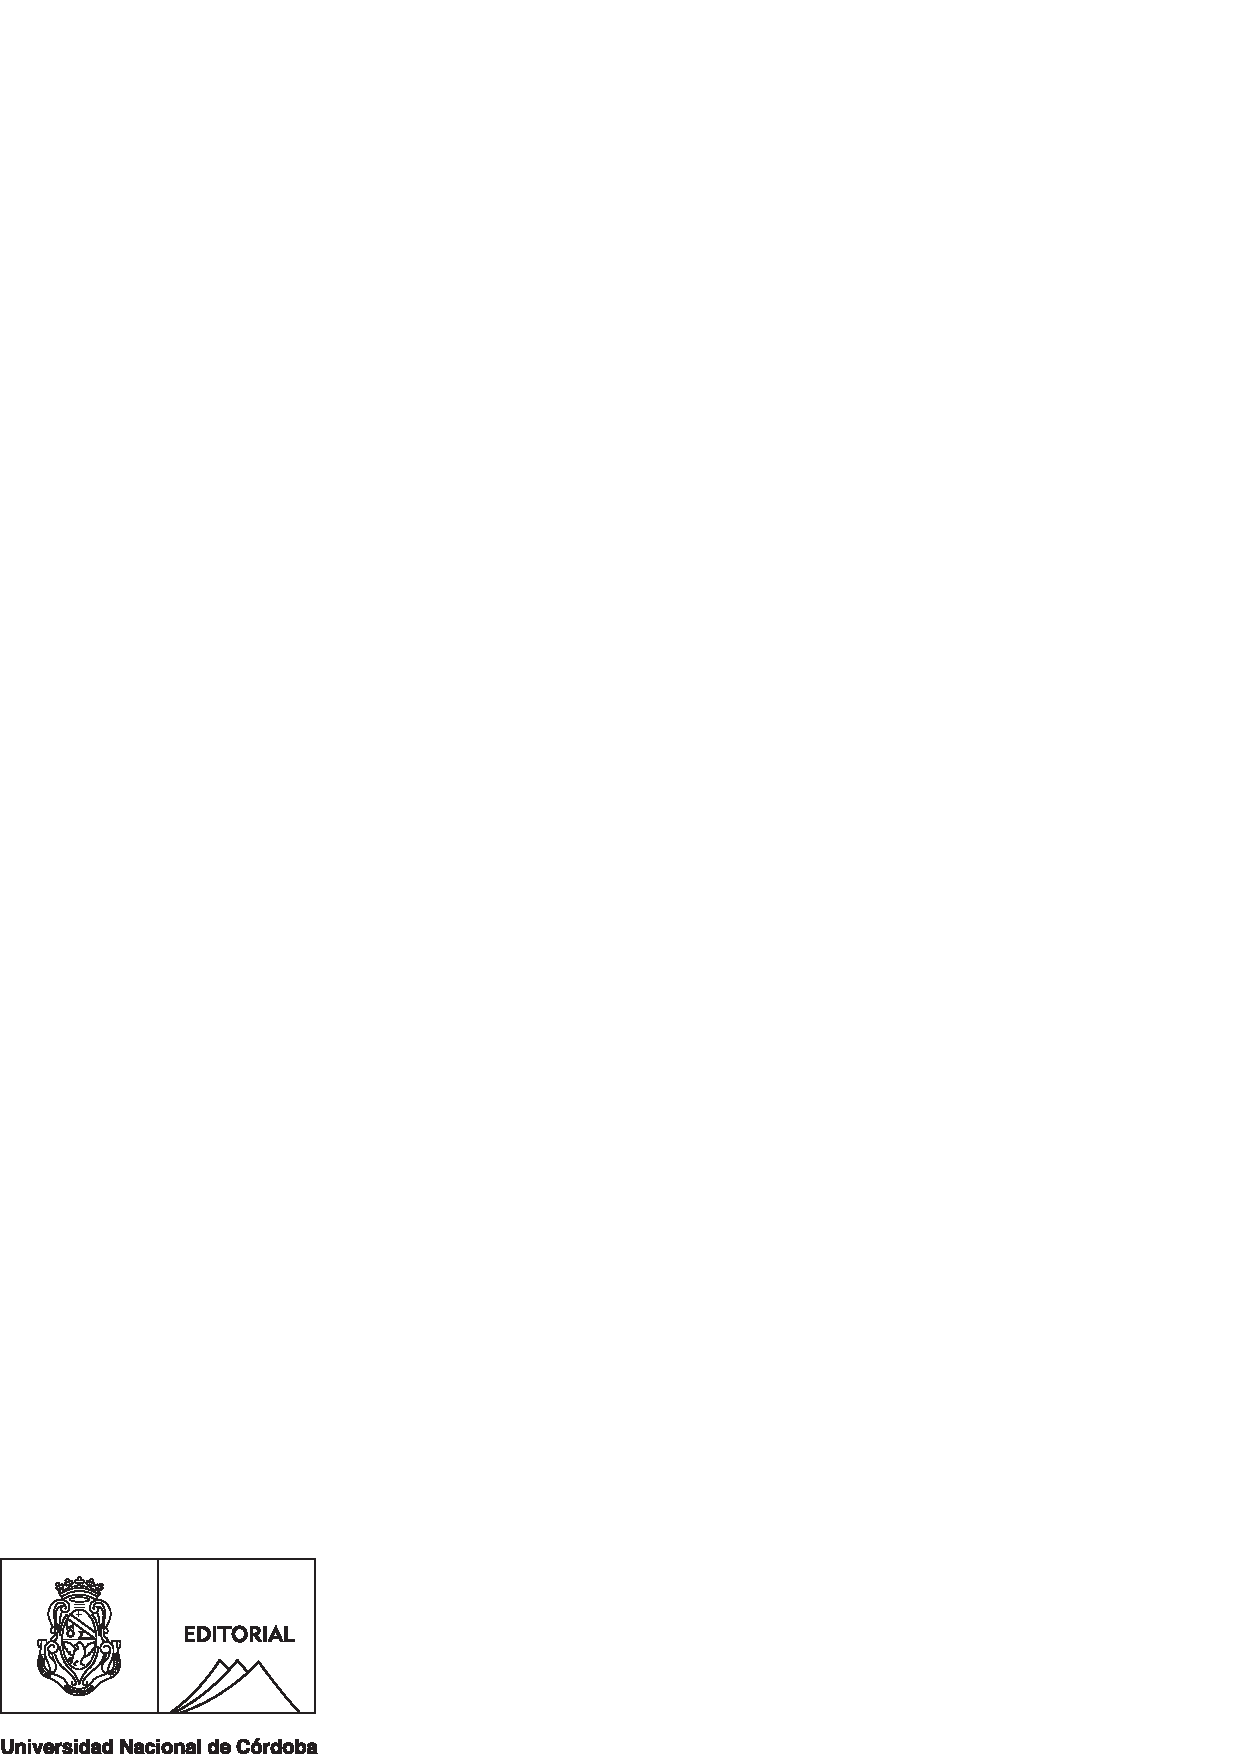
\includegraphics{Figure/logo.pdf}%
 \end{picture}
% }
    %\caption{Diagrama del operador dual.}
    %\label{fig:2_1}
%   \end{center}
% \end{figure}

%\maketitle

%\phantom{X}%\dag
\vspace*{4cm}
\begin{center}
 \textbf{\huge M\'etodos Matem\'aticos  de la F\'{\i}sica} \\
\vspace{1cm}
 \textbf{\Large \sc Oscar Reula}
\end{center}
\vfill
\vspace*{5cm}
\phantom{Y}
\vfill



%\part{}

% !TEX encoding = IsoLatin9
%%last modification 13-08-92

%\input format


\chapter*{Acknowledgements}

First of all, I want to thank Gloria Puente for supporting me throughout the time I wrote these notes, which took quite a bit of our shared hours, generally long nights.
Secondly, to Bernardo Gonz�lez Kriegel who converted the first versions of these notes to \LaTeX, doing a great job with much enthusiasm.
Also to Bob Geroch, with whom I discussed several topics of the notes and from whom I was also inspired through his writings and books, not only in content but also in style.
Finally, to several generations of students who stoically assimilated a large amount of the material from these courses in a very short time.
% 
% 
% \chapter*{Preface:}
% 
% These notes, now turned into a book, originated as an attempt to condense in one place a large set of ideas, concepts, and mathematical tools that I consider basic for the understanding and daily work of a physicist today.
% 
% It usually happens that if a problem is formulated from a physical origin, such as the description of some natural phenomenon, then it is well formulated, in the sense that a reasonable solution to it exists.
% This rule has generally been very fruitful and has particularly served as a guide to many mathematicians to make their way in unknown areas. But it has also served, particularly to many physicists, to work without worrying too much about formal aspects, whether analytical, algebraic, or geometric, and thus be able to concentrate on physical and/or computational aspects.
% Although this allows for the rapid development of some research, in the long run, it leads to stagnation because by proceeding in this way, one avoids facing problems that are very rich in terms of conceptualizing the phenomenon to be described. It is important to verify that the formulated problem has a mathematically and physically correct solution.
% 
% An example of this was the development, in the middle of the last century, of the modern theory of partial differential equations. Many of these equations arose because they describe physical phenomena: heat transmission, electromagnetic wave propagation, quantum waves, gravitation, etc.
% One of the first mathematical responses to the development of these areas was the Cauchy-Kowalevski theorem, which tells us that given a partial differential equation (under quite general circumstances), if an analytic function is given as data on a hypersurface (with certain characteristics), then there is a unique solution in a sufficiently small neighborhood of that hypersurface. It took a long time to realize that this theorem was not really relevant from the point of view of physical applications: there were equations admitted by the theorem such that if the data was not analytic, there was no solution! And in many cases, if they existed, they did not depend continuously on the given data, a small variation of the data produced a completely different solution. It was only in the middle of the last century that substantial progress was made on the problem, finding that there were different types of equations, hyperbolic, elliptic, parabolic, etc., that behaved differently and this reflected the different physical processes they simulated.
% Due to its relative novelty, this very important set of concepts is not part of the set of tools that many active physicists have, nor are they found in the textbooks usually used in undergraduate courses.
% 
% Like the previous one, there are many examples, particularly the theory of ordinary differential equations and geometry, without which it is impossible to understand many of the modern theories, such as relativity, elementary particle theories, and many phenomena of solid-state physics.
% As our understanding of the basic phenomena of nature advances, we realize that the most important tool for their description is geometry. This, among other things, allows us to handle a wide range of processes and theories with little in common with each other with a very reduced set of concepts, thus achieving a synthesis. These syntheses are what allow us to acquire new knowledge, since by adopting them we leave space in our minds to learn new concepts, which are in turn ordered more efficiently within our mental construction of the area.
% 
% These notes were originally intended for a four-month course. But in reality, they were more suited for an annual course or two semesters. Then, as more topics were incorporated into them, it became increasingly clear that they should be given in two semesters or one annual course.
% Basically, one course should contain the first chapters that include notions of topology, vector spaces, linear algebra, ending with the theory of ordinary differential equations. The task is considerably simplified if the students have previously had a good course in linear algebra. The correlation with physics subjects should be such that the course is prior to or concurrent with an advanced mechanics course.
% Emphasizing in it the fact that ultimately one is solving ordinary differential equations with a certain special structure.
% Using the concepts of linear algebra to find eigenmodes and the stability of equilibrium points. And finally using geometry to describe, albeit briefly, the underlying symplectic structure.
% 
% The second course consists of developing the tools to be able to discuss aspects of the theory of partial differential equations.
% It should be given before or concurrently with an advanced electromagnetism course, where emphasis should be placed on the type of equations that are solved (elliptic, hyperbolic), and the meaning of their initial or boundary conditions, as appropriate. Also using coherently the concept of distribution, which is far from being an abstract mathematical concept but is actually a concept that naturally appears in physics.
%  
% None of the content of these notes is original material, but some ways of presenting it are, for example, some simpler proofs than usual, or the way of integrating each content with the previous ones. Much of the material should be thought of as a first reading or an introduction to the topic and the interested reader should read the cited books, from which I have extracted much material, being these excellent and difficult to surpass.
% 
% 
% 
%

\tableofcontents
\listoffigures

%\garamond

\chapter*{Preface}

These notes, now turned into a book, originated as an attempt to condense in one place a large set of ideas, concepts, and mathematical tools that I consider basic for the understanding and daily work of a physicist today.

It usually happens that if a problem is formulated from a physical need, such as the description of some natural phenomenon, then it is well formulated, in the sense that a reasonable solution to it exists. This rule has generally been very fruitful and has particularly served as a guide to many mathematicians to make their way in unknown areas. But it has also served, particularly to many physicists, to work without worrying too much about formal aspects, whether analytical, algebraic, or geometric, and thus be able to concentrate on physical and/or computational aspects. Although this allows for the rapid development of some research, in the long run, it leads to stagnation because by proceeding in this way, one avoids facing problems that are very rich in terms of conceptualizing the phenomenon to be described. It is important to verify that the formulated problem has a mathematically and physically correct solution.

An example of this was the development, in the middle of the last century, of the modern theory of partial differential equations. Many of these equations arose because they describe physical phenomena: heat transmission, electromagnetic wave propagation, quantum waves, gravitation, etc. One of the first mathematical responses to the development of these areas was the Cauchy-Kowalevski theorem, which tells us that given a partial differential equation (under quite general circumstances), if an analytic function is given as data on a hypersurface (with certain characteristics), then there is a unique solution in a sufficiently small neighborhood of that hypersurface. It took a long time to realize that this theorem was not really relevant from the point of view of physical applications: there were equations admitted by the theorem such that if the data was not analytic, there was no solution! And in many cases, if they existed, they did not depend continuously on the given data, a small variation of the data produced a completely different solution. It was only in the middle of the last century that substantial progress was made on the problem, finding that there were different types of equations, hyperbolic, elliptic, parabolic, etc., that behaved differently and this reflected the different physical processes they simulated. Due to its relative novelty, this very important set of concepts is not part of the set of tools that many active physicists have, nor are they found in the textbooks usually used in undergraduate courses.

Like the previous one, there are many examples, particularly the theory of ordinary differential equations and geometry, without which it is impossible to understand many of the modern theories, such as relativity, elementary particle theories, and many phenomena of solid-state physics. As our understanding of the basic phenomena of nature advances, we realize that the most important tool for their description is geometry. This tool, among other things, allows us to handle a wide range of processes and theories with little in common among each other with a very reduced set of concepts, thus achieving a synthesis. These syntheses are what allow us to acquire new knowledge, since by adopting them we leave space in our minds to learn new concepts, which are in turn ordered more efficiently within our mental construction of the area.

These notes were originally intended for a four-month course. But in reality, they were more suited for an annual course or two semesters. Then, as more topics were incorporated into them, it became increasingly clear that they should be given in two semesters or one annual course. Basically, one course should contain the first chapters that include notions of topology, vector spaces, linear algebra, ending with the theory of ordinary differential equations. The task is considerably simplified if the students have previously had a good course on linear algebra. The correlation with physics subjects should be such that the course is prior to or concurrent with an advanced mechanics course. Emphasizing in it the fact that ultimately one is solving ordinary differential equations with a certain special structure. Using the concepts of linear algebra to find eigenmodes and the stability of equilibrium points. And finally using geometry to describe, albeit briefly, the underlying symplectic structure.

The second course consists of developing the tools to be able to discuss aspects of the theory of partial differential equations. It should be given before or concurrently with an advanced electromagnetism course, where emphasis should be placed on the type of equations that are solved (elliptic, hyperbolic), and the meaning of their initial or boundary conditions, as appropriate. Also using coherently the concept of \textit{distribution}, which is far from being an abstract mathematical concept but is actually a concept that naturally appears in physics.

None of the content of these notes is original material, but some ways of presenting it are: for example, some proofs that are simpler than usual, or the way some content is integrated with the previous ones. Much of the material should be thought of as a first reading or an introduction to the topic. The interested reader should consult the cited books, from which I have drawn upon a lot, being these excellent and difficult to surpass.

% !TEX encoding = IsoLatin9

%\input format

\chapter{Basic Concepts of Topology}

%\section{Topology}

\section{Introduction}

The notion of a set, while telling us that certain objects ---the elements that comprise it--- have something in common with each other, does not give us any idea of the {\it closeness} between these elements. On the other hand, if we consider for example the real numbers, this notion is present. We know, for example, that the number 2 is much closer to 1 than 423 is. The concept of a topology in a set that we will define below tries to capture precisely this notion of closeness which, as we will see, admits many gradations.

\defi: A {\bf topological space} consists of a pair $(X, \cT)$, where $X$ is a set and $\cT$ is a collection of subsets of $X$ satisfying the following conditions:

\begin{enumerate} \item The subsets $\emptyset$ and $X$ of $X$ are in \cT. \item If $O_{\lambda}$, $\lambda \in I$, is a one-parameter family of subsets of $X$ in \cT, then $\bigcup_I O_{\lambda}$ is also in \cT. \item If $O$ and $O'$ are in \cT, then $O \cap O'$ is also in \cT.

\end{enumerate}

For simplicity, we will often denote the topological space $(X, \cT)$ simply by $X$ when the topology is understood from context, as is common practice. 

The elements of \cT, subsets of $X$, are called the {\bf open subsets} of $X$. The set \cT itself is called a {\bf topology} on $X$. Condition 2) tells us that infinite unions of elements of \cT are also in \cT, while condition 3) tells us that in general only finite intersections remain in \cT. The following examples illustrate why this asymmetry exists, they also illustrate how giving a topology is essentially giving a notion of closeness between the points of the set in question.

\ejem: a) Let $\cT = \{\emptyset, X\}$, that is, the only open subsets of $X$ are the empty subset and the subset $X$. It is clear that this collection of subsets is a topology, as it satisfies the three required conditions. This topology is called the {\bf indiscrete topology} on $X$. We can say that, with this topology, the points of $X$ are arbitrarily close to each other, since if an open set contains one of them it contains all of them.

\ejem: b) Let \cT = \cP($X$), the collection of all subsets of $X$. Clearly, this collection also satisfies the conditions mentioned above and therefore it is also a topology on $X$, the so-called {\bf discrete topology on} $X$. We can say that in this one all the points are arbitrarily separated from each other since, for example, given any point of $X$ there is an open set that separates it from all the others, which consists of only the point in question.

\ejem: c) Let $X$ be the set of real numbers, \re, and let \\
$\cT = \{O \subseteq \re |\; \mathrm{if} \;r \in O, \, \exists \eps >0 \; \mathrm{such that if} \; |r - r'| < \eps, \; r' \in O}$, that is, the collection of open sets in the usual sense of the real numbers. Let's see that this collection satisfies the conditions to be a topology. Clearly, $\emptyset \in \cT$ (since it has no $r$), as well as \re$ \in \cT$ (since it contains all $r'$), and thus condition 1) is satisfied. Let us examine the second condition: let $r \in \bigcup_I O_{\lambda}$ then $r \in O_{\lambda}$ for some $\lambda$ and therefore there will exist $\eps >0 $ such that all $r'$ with $|r-r'| < \eps $ are also in $O_{\lambda}$, and therefore in $\bigcup_I O_{\lambda}$. 
Finally, the third condition: let $r \in O \cap O'$ then $r$ is in $O$ and therefore there will exist $\eps > 0$ such that all $r'$ with $|r-r'| < \eps $ will be in $O$; as $r$ is also in $O'$, there will exist $\eps'> 0$ such that all $r'$ with $|r-r'| < \eps'$ will be in $O'$. 
Let $\eps'' = \mathrm{min}\{\eps, \eps' \}$, then all $r'$ with $|r-r'| < \eps''$ will be in $O$ and in $O'$ and therefore in $O \cap O'$, so we conclude that this last set is also in \cT. $\re$ with this topology is called the {\bf real line}.

\ejer: In the real line, as defined in the previous example, find an infinite intersection of open sets that is not open.

\ejem: d) Let $X = \re \times \re \equiv \re^2$, that is, the Cartesian product of \re  with itself ---the set of all pairs $(x,y)$, with $x,y \in \re$--- and let \\
$\cT = \{O \in \reˆ2 |\; \mathrm{if} (x,y) \in O, \, \exists \eps >0 \mathrm{such that if} |x - x'|+|y-y'| < \eps, \; (x',y') \in O \}$. Following the previous example, it can be seen that this is also a topological space and that this is the topology we usually use in $\re^2$

\defi: A {\bf metric space} is a pair $(X,d)$ consisting of a set $X$ and a map $d: X \times X \to \re$, usually called \textbf{distance}, satisfying the following conditions for all $x, x', x'' \in X$:

\begin{enumerate} \item Non-negativity: $d(x,x') \geq 0$, with equality only when $x = x'$. \item Symmetry: $d(x,x')=d(x',x)$. \item Triangle inequality: $d(x,x') +d(x',x'') \geq d(x,x'')$. \end{enumerate}

\ejer: Prove that any metric space has a topology {\it induced} by its metric in a similar way to $\re$ in the previous example.

\ejer: Prove that, for any set, $d(x,y)=1$ if $x\neq y$ and $d(x,x)=0$ defines a distance. What topology does this distance induce on the set?

Clearly, a distance gives us a notion of closeness between points, in the precise form of a numerical value. A topology, by not generally giving us any number, gives us a much vaguer notion of closeness, but still generally interesting.

\subsection{Terminology}

We now give a summary of the usual terminology in this area, which is a direct generalization of the commonly used one.

\defi: We will call the {\bf complement}, $O^c$, of the subset $O$ of $X$ the subset of all elements of $X$ that are not in $O$.

\defi: We will say that a subset $O$ of $X$ is {\bf closed} if its complement $O^c$ is open.

\defi: A subset $N$ of $X$ is called a {\bf neighborhood of $x \in X$} if there is an open set $O_x$, with $x \in O_x$, contained in $N$.

\defi: We will call the {\bf interior} of $A \in X$ the subset $Int(A)$ of $X$ formed by the union of all open sets contained in $A$.

\defi: We will call the {\bf closure} of $A \in X$ the subset $Cl(A)$ of $X$ formed by the intersection of all closed sets containing $A$.

\defi: We will call the {\bf boundary} of $A \in X$ the subset $\partial A$ of $X$ formed by $Cl(A) - Int(A) \equiv Int(A)^c \cap Cl(A)$.

\ejer: Let $(X,d)$ be a metric vector space, prove that: \ a) $C^1_x = \{x'| d(x,x') \leq 1 \}$ is closed and is a neighborhood of $x$. \ b) $N^{\eps}_x = \{x' | d(x,x') < \eps \}$, $\eps >0$ is also a neighborhood of $x$. \ c) $Int(N^{\eps}_x) = N^{\eps}_x$ \ d) $Cl(N^{\eps}_x) = \{x' | d(x,x') \leq \eps \} $\ e) $\partial N^{\eps}_x = \{x' | d(x,x') = \eps \}$.

\ejer: Let $(X,\cT)$ be a topological space and $A$ a subset of $X$. Prove that: \ a) $A$ is open if and only if each $x \in A$ has a neighborhood contained in $A$. \ b) $A$ is closed if and only if each $x$ in $A^c$ (that is, not belonging to $A$) has a neighborhood that does not intersect $A$.

\ejer: Let $(X,\cT)$ be a topological space, let $A \in X$ and $x \in X$. Prove that: \ a) $x \in Int(A)$ if and only if $x$ has a neighborhood contained in $A$.\ b) $x \in Cl(A)$ if and only if every neighborhood of $x$ intersects $A$. \ c) $x \in \partial A$ if and only if every neighborhood of $x$ contains points in $A$ and points in $A^c$.

\section{Derived Concepts}

In the previous sections, we have seen that the concept of a topology leads us to a generalization of a series of ideas and derived concepts that we knew how to handle in $\re^n$, revealing that they did not depend on the usual distance used in these spaces (the so-called Euclidean distance). It is then worth asking if there are still other possible generalizations. In this and the next subsection, we will study two more of them. These in turn open up a vast area of mathematics, which we will not cover in this course but is very important in what concerns modern physics.

The first of these notions is \textit{continuity}.

\subsection{Continuous Maps}

\defi: Let $\fip :X \rightarrow Y$ be a map between two topological spaces (see the box below). We will say that the map $\fip$ is {\bf continuous} if given any open set $O$ of $Y$, $\fip^{-1}(O)$ is an open set of $X$.

\espa %%%%%%%%%%%%%%%%%%%%%%%%%%%%%%%%%%%%%%%%%%%%%%%%%%%%%%%%%%%%%%%%%%%%%%%%%

\recu{\defi: A {\bf map} $\phi:X \to Y$ between a set $X$ and another $Y$ is an assignment to {\it each} element of $X$ of an element of $Y$.

This generalizes the usual concept of a function. Note that the map is defined for every element of $X$ while, in general, its {\bf image}, that is, the set $\phi(X) \equiv \{y \in Y \; | \; \exists x \in X \text{such that} \phi(x) = y \}$, is not all of $Y$. In the case that it is, i.e. $\phi(X) = Y$, we will say that the map is {\bf surjective}. On the other hand, if it is fulfilled that $\phi(x) = \phi(\ti x) \Longrightarrow x=\ti x$, we will say that the map is {\bf injective}. In such a case, there exists the inverse map to $\phi$ between the set $\phi(X) \subset Y$ and $X$. If the map is also surjective then its inverse is defined on all of $Y$ and in this case, it is denoted by $\phi^{-1}:Y \to X$. It is also useful to consider the sets $\phi^{-1}(O) = \{ x \in X \; | \; \phi(x) \in O\}$, sometimes called the {\bf pre-image} of the set $O$ under $\phi$.

} %%%%%%%%%%%%%%%%%%%%%%%%%%%%%%%%%%%%%%%%%%%%%%%%%%%%%%%%%%%%%%%%%%%%%%%%%%%%

\espa

Clearly, the previous definition only uses topological concepts. Does it have anything to do with the usual {\sl epsilon-delta} definition used in $\re^n$? The answer is affirmative, as we will see below in our first theorem. But first, let's see some examples.

\ejem: a) Let $X$ and $Y$ be any topological spaces and let the topology on $X$ be the discrete one. Then any map between $X$ and $Y$ is continuous. Indeed, for any open set $O$ in $Y$, $\fip^{-1}(O)$ is some subset in $X$, but in the discrete topology, every subset of $X$ is an open set.

\ejem: b) Let $X$ and $Y$ be any topological spaces and let the topology on $Y$ be the indiscrete one. Then any map between $X$ and $Y$ is also continuous. Indeed, the only open sets in $Y$ are $\emptyset$ and $Y$, but $\fip^{-1}(\emptyset) = \emptyset$, while $\fip^{-1}(Y)=X$, but whatever the topology of $X$, $\emptyset$ and $X$ are open sets.

From the previous examples, it might seem that our definition of continuity is not very interesting. But that is because we have taken cases with the {\sl extreme} topologies. It is in the intermediate topologies where the definition becomes more useful.

\ejem: c) Let $X$ and $Y$ be real lines, and let $\fip : X \to Y$ be a map such that $\fip(x) = 1$ if $x \geq 0$, $\fip(x) = -1$ if $x < 0$. This map is not continuous because, for example, while the interval $I = (1/2, 3/2) \subseteq Y$ is open, its pre-image $\fip^{-1}(I) = \{x \, | \, x \geq 0 \}$ is not open.

\bteo The map $\fip:X \to Y$ is continuous if and only if given any point $x \in X$ and any neighborhood $M \subseteq Y$ of $\fip(x)$, there exists a neighborhood $N \subseteq X$ of $x$ such that $\fip(N) \subset M$. \eteo

This theorem provides an equivalent definition of continuity that is much closer to the intuitive concept of continuity.

\bpru

Suppose $\fip$ is continuous. Le    t $x$ be a point of $X$, and $M \subseteq Y$ a neighborhood of $\phi(x)$. By definition of neighborhood, there exists an open set $O \subset M$ in $Y$ and containing $\phi(x)$. By continuity, $N = \fip^{-1}(O)$ is an open set of $X$, and as it contains $x$, it is a neighborhood of $x$. It is then fulfilled that $\fip(N) \su O \su M$. Now to prove the reciprocal, suppose that given any point $x \in X$ and any neighborhood $M$ of $\fip(x)$, there exists a neighborhood $N$ of $x$ such that $\fip(N) \subset M$. Then let $O$ be any open set of $Y$, we must now show that $\fip^{-1}(O)$ is an open set of $X$. Let $x$ be any point of $\fip^{-1}(O)$, then $\fii (x) \in O$ and therefore $O$ is a neighborhood of $\fii (x)$, therefore there exists a neighborhood $N$ of $x$ such that $\fip(N) \su O$ and therefore $N \su \fip^{-1}(O)$. But then $\fip^{-1}(O)$ contains a neighborhood of each of its points and therefore it is open.
\epru

\ejer: Let $\phi : X \to Y$ and $\psi : Y \to Z$ be continuous maps, prove that the composite map $\psi \circ \phi : X \to Z$ is also continuous. (Composition of maps preserves continuity.)

\espa %%%%%%%%%%%%%%%%%%%%%%%%%%%%%%%%%%%%%%%%%%%%%%%%%%%%%%%%%%%%%%%%

\recu{{\bf \yaya{Induced Topology}:} \espa

Let $\phi$ be a map between a set $X$ and a topological space $\{Y,\cT \}$. This map naturally provides, that is, without the help of any other structure, a topology on $X$, denoted by $\cT_{\phi}$ and called the {\bf topology induced} by $\phi$ on $X$. It is given by $\cT_{\phi} = \{O \subset X \;| \; O = \phi^{-1}(Q), ; Q \in \cT \}$, that is, $O$ is an open set of $X$ if there exists an open set $Q$ of $Y$ such that $O = \phi^{-1}(Q)$. In other words, the open sets in $X$ are the pre-images of all the open sets in $Y$. Note that under this topology on $X$, the map $\phi$ is automatically continuous. In fact, it is by construction the ``minimal'' topology on $X$ that renders $\phi$ continuous. \espa

\ejer: Prove that this construction really defines a topology.

Not all topologies thus induced are of interest and, in general, they depend strongly on the map, as shown by the following example:

\ejem:

\noi a) Let $X=Y=\re$ with the usual topology and let $\phi: \re \to \re$ be the function $\phi(x) = 17$ $\forall x \in \re$. This function is clearly continuous with respect to the topologies of $X$ and $Y$, those of the real line. However, the topology induced on $X$ by this map is the indiscrete one!: $\cT_{\phi} = \{\emptyset, X\}$. Interestingly, this ``loss'' of topological information can be intuitively associated to the information lost by $\phi$ in mapping the whole $\re$ to a single point, $17$. In fact, $\phi$ would be continuous with respect to \textit{any} topology on $X$, so its continuity is not very interesting, as it does not tell us anything about the underlying topology.

\noi b) Let $X$ and $Y$ be as in a) and let $\phi(x)$ be an invertible map, then $\cT_{\phi}$ coincides with the topology of the real line.

} %%%%%%%%%%%%%%%%%%%%%%%%%%%%%%%%%%%%%%%%%%%%%%%%%%%%%%%%%%%%

\subsection{Compactness}

The second generalization that we are interested in corresponds to the concept of {\it compactness}.
For this, we introduce the following definition:
let $X$ be a set, $A$ a subset of $X$, and $ C = \{ A_{\lambda} \}$
a collection of subsets of $X$ parameterized by a continuous
or discrete variable $\lambda$. We say that this collection {\bf covers}
$A$ if $A \subset \cup_{\lambda}A_{\lambda}$. In such a case, we also say that $C$ is a {\bf cover} of $A$. When $A$ is a topological space and the sets $\{ A_\lambda \}$ are open, we say that $C$ is an {\bf open cover} of $A$. Finally, a subcollection of $C$ that also covers $A$ is called a {\bf subcover}. 

\defi: We say that a topological space $A$ is {\bf compact} if given any collection
$\{A_{\lambda}\}$ of {\it open sets} that covers $A$, there exists a {\it finite}
subcollection of these $A_{\lambda}$ that also covers $A$.

\ejem: a) Let $X$ be an infinite set of points with the discrete topology.
Then a cover of $X$ consists, for example, of all subsets of the form $\{x\}$, with $x \in X$. Since the topology of $X$ is
discrete, any cover is an open cover. But no finite number of the sets $\{x\}$
cover all of $X$, therefore $X$ is not compact in this case.
Clearly, if $X$ had only a finite number of elements
it would always be compact, regardless of its topology.

\ejem: b) Let $X$ be any set with the indiscrete topology.
Then $X$ is compact. The only open sets of this set are
$\emptyset$ and $X$, so any open cover has $X$ as
one of its members and this alone is enough to cover $X$.

Thus, we see that this property strongly depends on the topology
of the set. The relation with the intuitive concept of compactness
is clear from the following example and exercise.

\ejem: c) Let $X$ be the real line and $A = (0,1)$. This subset is not compact
because, for example, the following is an open cover of $A$ that has no finite subcover: $\{ A_n = (\frac{1}{n}, \frac{n-1}{n}) \colon n \in \mathbb{N}\}$

\ejer: Let $X$ be the real line and $A = [0,1]$. Prove that $A$ is compact.

\bpru

Let $\{A_{\lambda}\}$ be an open cover of $[0,1]$. In particular, it covers any subinterval $[0,x]$ with $x \in [0,1]$. Consider the set $S$ of all $x$ such that $[0,x]$ is covered by \textit{finitely} many $A_\lambda$, and let $a \in [0,1]$ be the least upper bound 
of this set. Because $0$ is covered by some single $A_\lambda_0$, then $0 \in S$. Besides, by definition, $S$ is bounded above by $1$. Therefore, $S$ is a non-empty upper-bounded real set, so by the least-upper-bound property of $\re$ it has a least upper bound. Let $a$ be that number and $A_{\lambda_0}$ be an element of the cover
such that $a \in A_{\lambda_0}$. Because $a$ is the \textit{least} upper bound of $S$, there must be some $a'<a$ in $A_{\lambda_0}$ such that $a \in S$. Therefore, $[0,a']$ has a finite subcover, and the union of this finite subcover with $\{A_\lambda_0\}$ provides a finite subcover of $[0,a]$. Now we want to show that $a=1$. So let us assume $a<1$ and take $b \in A_\lambda_0$ such that $a < b < 1$. Then $[0,b]$ is covered by the same finite subcover constructed for $[0,a]$, implying $b \in S$. But this contradicts the fact that $a$ is an upper bound of $S$, so we conclude that $a=1$. 
\epru

Now let's see the relation between the two derived concepts of
Topology, namely the continuity of maps between topological
spaces and compactness. The fact that a map between
topological spaces is continuous implies that this map is special,
in the sense that {\it it carries or conveys information about the respective
topologies and preserves the topological properties of the sets
it associates}. This is seen in the following property, which ---as shown by
the following example--- is very important.

\bteo
Let $X$ and $Y$ be two topological spaces and $\phi: X \to Y$ a continuous
map between them. Then if $A$ is a compact subset of $X$, 
$\phi(A)$ is a compact subset of $Y$.
\eteo

\pru:
Let $\{O_{\lambda}\}$ be a collection of open sets in $Y$ that cover $\phi(A)$.
Then the collection $\{\phi^{-1}(O_{\lambda})\}$ covers $A$, but $A$ is
compact and therefore there will be a finite subcollection 
$\{\phi^{-1}(O_{\tilde{\lambda}}\})$
of the former that also covers it. Therefore, the finite subcollection
$O_{\tilde{\lambda}}$ will also cover $\phi(A)$. Since this is
true for any open cover of $\phi(A)$
we conclude that $\phi(A)$ is compact.

\ejem: Let $A$ be a compact topological space and let $\phi:A \to \re$ be a continuous map between $A$ and the real line. $\phi(A)$ is then a compact real set
and therefore a closed and bounded set, but
then this set will have a maximum and a minimum, that is, the
map $\phi$ reaches its maximum and minimum in $A$.


Finally, another theorem of fundamental importance about compact sets,
which shows that they have another property that makes them
very interesting. For this, we introduce the following definitions,
which also only use topological concepts.
A {\bf sequence} in a set $X$, 
$\{x_n\} = \{x_1, x_2, ...\}$, with $x_n \in X$, is a map
from $\mathbb{N}$ to this set.
Given a sequence $\{x_n\}$ in a topological space $X$, we say that 
$x \in X$ is a {\bf limit point} of this sequence if given
any open set $O \subseteq X$ containing $x$ there exists a number $N$
such that for all $n > N$, $x_n \in O$. We say that 
$x \in X$ is an {\bf accumulation point} of this sequence if given 
any open set $O \subseteq X$ containing $x$, infinitely many elements of the
sequence also belong to $O$. 

\espa

\ejer: Find an example of a sequence in some topological
space with different limit points. 

\espa
%\newpage

\bteo
Let $A$ be compact. Then every sequence in $A$ has an accumulation point.
\eteo

\espa

\bpru
Suppose ---contrary to the theorem's assertion--- that
there exists a sequence $\{x_n\}$ in $A$ without any accumulation points.
That is, given any point $x \in A$ there exist a neighborhood $O_x$
containing it and a number $N_x$ such that if $n > N_x$ then $x_n \notin
O_x$. Since this is valid for any $x$ in $A$, the collection of
sets $\{ O_x | x \in A \}$ is an open cover of $A$, but $A$ is compact and therefore
it has a finite subcover.
Let $N$ be the maximum among the $N_x$ of this finite subcover. But then
$x_n \notin A$ for all $n > N$ which is absurd.  
\epru

\ejer: Prove that compact sets in the real line are the
closed and bounded ones.


We can now ask the inverse question: if $A \subset X$ is
such that every sequence has accumulation points, is it true
then that $A$ is compact? An affirmative answer would give us
an alternative characterization of compactness, and this is
affirmative for the case of the real line. In general, however, the answer is
negative: there are topologies in which every sequence in a
set has accumulation points in it, but this set is not
compact. However, all the topologies we will see are {\bf second countable} [See box] and in these
the answer is affirmative.

In the real line, it is true that if $x \in \re $ is an accumulation point of a sequence $\{x_n\}$ then there exists a {\bf
subsequence}, $\{\tilde{x}_n\}$ (that is, a restriction of the
map defining the sequence to an infinite subset of $\mathbb{N}$) having $x$ as a limit point. This is also not
true in the generality of topological spaces, but it is if we consider only those that are {\bf first countable} [See box]. All the spaces we will see in this
course are first countable.

\espa 
\vfill   %%%%%%%%%%%%%%%%%%%%%%%%%%%%%%%%%%%%%%%%%%%%%%%%%%%%%%%%%%%%%%%%%%%%%%

\recu{
{\bf *\yaya{Countability of topological spaces.}}
\espa

\defi: We say that a topological space $\{X,\cT\}$ is {first countable}
if for each $p \in X$ there exists a countable collection of open sets $\{O_n\}$ such that for every neighborhood $N$ of $p$ there exists $i$ such that $O_i \subset N$.

\espa

\defi: We say that a topological space $\{X,\cT\}$ is {second countable}
if there is a countable collection of open sets such that any open set of $X$ can be expressed 
as a union of sets from this collection.

\espa
\ejem:

\noi a) $X$ with the indiscrete topology is first countable.

\noi b) $X$ with the discrete topology is first countable. And second countable if and only if its elements are countable.

\espa
\ejer: Prove that the real line is first and second countable. Hint: For the
first case, use the open sets $O_n = (p - \frac{1}{n}, p + \frac{1}{n})$ and for the second 
$O_{pqn} = (\frac{p}{q} - \frac{1}{n}, \frac{p}{q} + \frac{1}{n})$

}  
%%%%%%%%%%%%%%%%%%%%%%%%%%%%%%%%%%%%%%%%%%%%%%%%%%%%%%%%%%%%%%%%%%%%%%
\espa

\recu{
{\bf *\yaya{Separability of topological spaces.}}
\espa

\defi: A topological space $X$ is Hausdorff if given any pair of points of $X$, $x$ and $y$,  there exist neighborhoods $O_x$ and $O_y$ such that $O_x \; \cap O_y = \emptyset$.

\ejem:

\noi a) $X$ with the indiscrete topology is not Hausdorff.

\noi b) $X$ with the discrete topology is Hausdorff.

\ejer: Find a topology such that the integers are Hausdorff and compact.

\ejer: Prove that if a space is Hausdorff then if a sequence has a limit point, it is unique.

\ejer: Let $X$ be compact, $Y$ Hausdorff, and $\phi :  X \to Y$ continuous. Prove that the images of closed sets are closed. Find a counterexample if $Y$ is not Hausdorff. 
}

\recubib{
This chapter is essentially a condensed version of Chapters \textbf{26, 27, 28, 29,} and \textbf{30} of \cite{Geroch}, see also \cite{Kelley}, \cite{Wald}, and \cite{Isham}.
Topology is one of the most fascinating branches of mathematics, if you delve deeper you will be captivated! Of particular interest in physics is the notion of \textit{Homotopy}, a good place to understand these ideas is Chapter \textbf{34} of \cite{Geroch}.       }

\vfill
%\end{document}
%\end


%%% Local Variables: 
%%% mode: latex
%%% TeX-master: "apu_tot"
%%% End:

\chapter{Linear Algebra}


\section{Vector Spaces}

\defi:
A {\bf Real Vector Space} consists of three things:
--- $i$) a set, $V$, whose elements will be called {\bf vectors};
$ii$) a rule that assigns to each pair of vectors, $\ve{v}$,
$\ve{u}$, a third vector which we will denote by $\ve{v+u}$ and call
their {\bf sum}; and $iii$) a rule that assigns to each vector, $\ve{v}$ and
to each real number $a$, a vector which we will denote by $a\ve{v}$ and
call the {\bf product} of $\ve{v}$ with $a$, all subject to
the following conditions:

\begin{itemize}

\item[1.a)] For any pair of vectors $\ve{u}$, $\ve{v} \in V$
it holds that,
\beq
\ve{u} + \ve{v} = \ve{v} + \ve{u}
\eeq

\item[1.b)] There exists in $V$ a unique element called {\bf zero} and denoted by $\ve{0}$,
such that 

\beq
\ve{0+v = v} \;\forall \ve{v}  \in V.
\eeq

\item[1.c)] For any vector $\ve{u} \in V$ there exists a unique
vector in $V$, denoted $-\ve{u}$, such that,
\beq
\ve{u} + (-\ve{u}) = \ve{0}
\eeq

\item[2.a)] For any pair of real numbers $a$ and $a'$ and any vector 
$\ve{v}$ it holds that,
\[
a(a'\ve{v}) = (aa')\ve{v}.
\]

\item[2.b)] For any vector 
$\ve{v}$ it holds that,
\[
1\ve{v} = \ve{v}.
\]

\item[3.a)] For any pair of real numbers $a$ and $a'$ and any vector 
$\ve{v}$ it holds that,
\[
(a+a')\ve{v} = a\ve{v} + a'\ve{v}.
\]

\item[3.b)] For any real number $a$ and any pair of vectors
$\ve{v}$ and $\ve{v}'$ it holds that,
\[
a(\ve{v}  + \ve{v}') = a\ve{v} + a\ve{v}'.
\]

\end{itemize}

The first conditions involve only the rule of addition; these are actually the rules that 
define a group, a structure we will revisit in a later chapter, where addition represents the product between elements of the group.
The next conditions involve only the rule of multiplication, while
the last two deal with the relation between these two operations. As we will see with examples later, real numbers can be replaced by any field, such as rationals, $\Rationals$, integers, $\Integers$, complex numbers, $\Complex$, and even finite fields.

\espa

\ejem: The set of all $n$-tuples of real numbers with the
usual operations of component-wise addition and multiplication.
This space is denoted by $\re^n$.

\ejem: Let $S$ be any set and let $V$ be the set of all functions
from $S$ to the reals, $\ve{v}:S \to \re$, with the following
operations of addition and multiplication: the sum of the function $\ve{v}$ with
the function $\ve{v}'$ is the function (element of $V$) that assigns to the element
$s \in S$ the value $\ve{v}(s) + \ve{v}'(s)$. The product of
$a \in \re$ with the function $\ve{v}$ is the function that assigns to $s \in S$
the value $a\ve{v}(s)$.
This example will appear very often in the following chapters.

\defi: We will say that a set of vectors $\{\ve{e_i}\}$, $i=1, \ldots ,n$,
are {\bf linearly independent}~\index{linear!independence} 
if $\sum_{i=1}^{n} a^i \ve{e_i} = \ve{0}$ $a^i \in \re$ $\Longrightarrow $ $a^i = 0$, $i= 1, \ldots ,n$;
that is, if any non-trivial linear combination of these vectors gives us a non-zero vector. 

\defi: The {\bf span} of a set of vectors $\{\ve{u_{i}}\}$ is the set of all possible linear combinations of these elements. They generate a subspace of $V$, which we will denote by $Span\{\ve{u_{i}}\}\subset V$. 

If a finite number of linearly independent vectors, 
$n$, are sufficient to span $V$ (that is, if 
any vector in $V$ can be obtained as a linear combination of 
these $n$ vectors) then we will say that these vectors form a {\bf basis} of 
$V$ and that the {\bf dimension}~\index{dimension} of $V$ is $n$, $\dim V = n$.
\espa

\ejer: Show that given a vector $\ve{v} \in V$ and a basis of V, $\{\ve{e_i}\}$ $i=1, \ldots ,n$, the linear combination of the basis vectors that equals $\ve{v}$ is unique. That is, if 
$\ve{v} =  \sum_i v^i \ve{e_i} $ and $\ve{v} = \sum_i \tilde{v}^i \ve{e_i} $, then $v^i=\tilde{v}^i$ for all
$i=1, \ldots ,n$.

\ejer: If we have two bases of a real vector space $V$ of dimension $n$, $\{\ve{e_i}\}$ and $\{\ve{\tilde{e}_i}\}$, we can write the elements of one in terms of the other, 

\[
\ve{\tilde{e}_j} = \sum_i P_{j}{}^i \ve{e_i}, \;\;\;\;\;\; \ve{e_i} = \sum_l R_{i}{}^l \ve{e_l},
\]
%
where $P_{j}{}^i$ and $R_{i}{}^l$ are the coefficients of two real $n \times n$ matrices. Prove that $R_{i}{}^l = P^{-1}_{i}{}^l $.

\ejer:
Let $S = \{s_1,s_2,\dots,s_n\}$ be a finite set. Find a basis 
of the vector space of all functions from $S$ to $\re$. 
What is the dimension of this space?

\ejer: Show that the dimension of a vector space $V$ is well defined, i.e. it does not depend on
the basis used to define it. 

Note that, in the previous example, $V$ has finite dimension\footnote{That is, a finite number of linearly independent vectors span $V$.} because $S$ is finite. If $S$
had an infinite number of elements, $V$ would have an infinite basis and we would say that the dimension of $V$ would be infinite. In the rest of this Chapter, we will assume the vector spaces are finite-dimensional, unless otherwise stated.

Let $V$ be a real vector space of dimension $n$ and a basis of it, $\{\ve{e_i}\}$ $i=1, \ldots ,n$. 
Given an $n$-tuple of real numbers, $\{c^{i}\}$, we then have determined an element of $V$, 
that is, the vector,  $\ve{v}=\sum_{i=1}^{n} c^{i}\ve{e_i}$. 
On the other hand, we have seen in a previous exercise that, given any vector, it determines a unique $n$-tuple of real numbers, the coefficients of $\ve{v}$ in that basis. 
We see that we then have an invertible map between $V$ and the space of $n$-tuples, $\re^{n}$.
This map is linear, assigning to the sum of two vectors $\ve{v}$ and $\ve{\tilde{v}}$ the $n$-tuple sum of the respective $n$-tuples. This map depends on the basis, but it still tells us that finite-dimensional real vector spaces do not hold many surprises: they are always copies of $\re^{n}$.

\subsection{Covectors and Tensors}
\label{sub:Covectors_and_Tensors}

Let $V$ be a vector space of dimension $n$. 
Associated with this vector space, consider the set of linear maps from $V$ to $\re$,
$V^*=\{\ve{\omega}:V\to \re : \ve{\omega} \text{is linear}\}$. 
This is also a vector space, called the {\bf dual space to $V$}~\index{dual space}, 
or {\bf space of covectors},~\index{covectors} with addition and multiplication given by: 

\[
(\ve{\omega}+\alpha \ve{\tau})(\ve{ v})=
\ve{\omega}(\ve{ v})+\alpha \ve{\tau}(\ve{ v})\;\;\;\;\forall\;\ve{v}\in V
\]
%
with  $\ve{\omega},\ve{\tau}\,\in V^*\;,\,\alpha \in \re$. 

What is the dimension of $V^*$? 
Note that if
$\{\ve{ e}_i\}$ $i=1,\ldots,n$ is a basis of $V$, we can define $n$
elements $\ve{ \theta^i}  \in V^*$ by the relation 
\beq
\ve{ \theta^i}(\ve{ e}_j)=\delta^i_{\;j}.
\eeq
That is, we define the action of $\ve{ \theta^i}$ on the basis vectors $\ve{e_j}$
as in the equation above, and then extend its action to any vector in $V$ by writing this element in the basis $\{\ve{ e}_i\}$
and using the fact that the $\ve{ \theta^i}$ act linearly on vectors.
  
It can be easily seen that any covector $\rho \in V^*$ can be obtained
as a linear combination of the covectors $\{\ve{\theta^j}\}$,
$j=1,\ldots,n$ and that these are linearly independent, therefore
they form a basis and thus the dimension of $V^*$ is also $n$. We will call this basis the {\bf co-basis} of the basis $\{\ve{e_i}\}$.
\espa

\ejer: Prove that $V^*$ is a vector space and that the $\{\ve{ \theta^i}\}$
really form a basis.

\ejer: Prove that if $\ve{v} = \sum_{i=1}^{n} v^i \ve{e}_i$ then the coefficients can be obtained by acting on $\ve{v}$ with the covectors $\ve{\theta}^i$, that is,

\[
v^i = \ve{\theta}^i(\ve{v}).
\]

\ejer:
Let $V$ be the space of functions $S \to \re$, where $S$ is a finite set with $n$ elements.
Let a basis of $V$ be given by:

\[
\ve{e}_i (a) := \left\{
\begin{array}{cl}
1 & \text{if} \;\; a \;\; \text{is the i-th element of} S \\
0 & \text{otherwise}
\end{array}
\right.
\]
%
Find the corresponding co-basis of its dual space. 

Since $V$ and $V^*$ have the same dimension, they are, as vector
spaces, isomorphic. For any basis of $V$ have an associated co-basis of $V^*$, and we can extend this to associate to any vector in $V$ a covector in $V^*$.
However, this association is dependent on the choice of basis for $V$: if we choose a different basis, the association would be completely different. 
Then, this association is not intrinsic to the vector space. Since there is no \textit{natural} map that identifies $V$ with $V^*$, we have to consider them as intrinsically different, although isomorphic. 

What happens if we now take the dual of $V^*$? Will we get another intrinsically different vector space? The answer is negative, since \textit{there is} a natural identification
between $V$ and its double dual $V^{**}$.

Indeed, to each $\ve{v}\in V$ we can associate an element $\ve{
X}_v$ of
$V^{**}$ (that is, a linear functional from $V^*$ to $\re$) in the
following way: $\ve{X}_v(\omega):=\omega(\ve{v}) \;\;\;\forall
\;\;\omega\in V^{*}$. $\ve{X}_v(\omega)$ is sometimes called, unsurprisingly, the \textit{evaluation map} on $\ve{v}$. That is, the element $\ve{X}_v$ of $V^{**}$
associated with $\ve{ v}\in V$ is the one that, when acting on any
covector $\omega$, gives the number $\omega (\ve{v})$. Note that $\ve{X}_v$ acts
linearly on the elements of $V^*$ and therefore is an element
of $V^{**}$. Are there elements of $V^{**}$ that do not come from some
vector in $V$? The answer is negative, since the map  $\ve{X_v}:V\to V^{**}$ is
injective [$\ve{X}_v(\omega)=0\;\;\forall \; \omega\Longrightarrow \ve{v}=0$] and
therefore\footnote{Denoting by $\ve{X}_V$ the image by $\ve{X}_{(\cdot)}$ 
of $V$.} $\dim \ve{X}_V = \dim V$.
On the other hand $\dim V^{**} = \dim V^*$ since $V^{**}$ is the dual of $V^*$ and thus 
$\dim V = \dim V^* = \dim V^{**}$, which indicates that the map in question is also 
surjective and therefore invertible.
This allows us to \textit{identify}
$V$ and $V^{**}$ and conclude that by dualizing further we will not be able
to construct any more interesting vector spaces. In the case where the dimension of the vector space is not finite, this is no longer true and there are cases ---frequently used in physics--- where $\ve{X}_V \subset V^{**}$ strictly.
\espa

\ejer: Given a basis of $V$, $\{\ve{e_{i}}\}$, and the corresponding co-basis, $\{\ve{\theta^{j}}\}$, define the co-co-basis of $V^{**}$, $\{\ve{E_{i}}\}$. 
Find the relation between the components of a vector of the form $X_{v}$ in the basis $\{\ve{E_{i}}\}$ and 
those of the vector $\ve{v}$ in the basis $\{\ve{e_{i}}\}$.

\ejer: Prove that indeed $\dim \ve{X}_V = \dim V$.

However, nothing prevents us from also considering \index{multilinear maps}
{\bf multilinear maps}\footnote{That is, maps that are separately linear in each 
of their arguments.} 
from $\underbrace{V\times V\times\cdots\times V}_{k\;\mbox{times}}$ to $\re$,
or more generally,

\[
\underbrace{V\times\cdots\times V}_{k\;\mbox{times}}
\times\underbrace{ V^*\times \cdots\times V^*}_{l\;\mbox{times}} \to \re.
\]
%
The set of these maps, for each given pair $(k,l)$, is also a vector 
space with the obvious operations and its elements are called
{\bf tensors of type ${l\choose k}$}~\index{tensors!type}.

\ejer: What is the dimension of these spaces as a function of their type ${l \choose k}$?

\noi\yaya{Note}:
In finite dimension, it can be shown that any tensor of type ${l \choose k}$
can be written as a linear combination of elements of the Cartesian product of $k$ copies of $V^*$ and $l$ copies of $V$ 
---where we have identified $V$ with $V^{**}$---. 
For example, if $\ve{t}$ is of type ${0 \choose 2}$, ---that is, a map that has as arguments two covectors---, 
then given a basis $\{\ve{e_{i}}\}$ of $V$, and the corresponding basis of $V^{**}$, $\{\ve{E}_{i}\}$ there will be $n \times n$ real numbers $t^{ij}$, $i=1, \ldots ,n$ such that 
\beq
\ve{t}(\ve{\sigma},\ve{\omega}) = 
\sum_{i,j=1}^{n} t^{ij} \ve{E_i}(\ve{\sigma})\ve{E_j}(\ve{\omega})
=
\sum_{i,j=1}^{n} t^{ij} \ve{\sigma}(\ve{e_i}) \ve{\omega}(\ve{e_j}), 
\;\;\;\; \forall \ve{\sigma},\;\ve{\omega} \in V^*.
\eeq
%
But the set of linear combinations of Cartesian products of
$k$ copies of $V^*$ and $l$ copies of $V$ is also a vector
space, it is called the {\bf outer product}~\index{outer product} 
of  $k$ copies of $V^*$ and $l$ copies of $V$ and is denoted by 

\[
\underbrace{V^*\otimes V^*\otimes\cdots\otimes V^*}_{k\;\mbox{times}}
\otimes\underbrace{ V\otimes \cdots\otimes V}_{l\;\mbox{times}}.
\]
%
Therefore, tensors can also be considered as elements
of these outer products.

\ejem: a) Let $\ve{ t}$ be of type ${0 \choose 2}$, that is, $\ve{ t}\in\;V^*\otimes V^*$. 
This is a bilinear map from $V\times V$ to $\re$, $\ve{ t}(\ve{v},\ve{u})\in \re$. Let
$\ve{ t}$ be symmetric $[\ve{ t}(\ve{v},\ve{u})=\ve{ t}(\ve{u},\ve{v})]$ and non-degenerate 
[$\; \ve{ t}(\ve{v},\cdot)= 0
\in V^*\Longrightarrow \ve{v}=0$]. 
Since $\ve{ t}$ is non-degenerate, it defines an invertible map between $V$ and its dual. 
Indeed, given $\ve{v} \in V$, $\ve{t}(\ve{v},\cdot)$ is an element of $V^*$. 
But if $\ve{v}$ and $\ve{\tilde{v}}$ determine the same element of $V^*$, that is, if $\ve{ t}(\ve{v},\ve{u}) = \ve{ t}(\ve{\tilde{v}},\ve{u}) \;\; \forall \; \ve{u} \in V$ then $\ve{v}=\ve{\tilde{v}}$, which can be seen by taking $\ve{u} = \ve{v} - \ve{\tilde{v}}$ and using that $\ve{t}$ is non-degenerate. Since the dimensions of $V$ and $V^{*}$ are equal, the map thus defined is invertible.

\ejem: b) Let $\ve{\varepsilon}$ be a tensor of type ${0 \choose n}$ such that \beq \ve{\varepsilon} (\ldots,\underbrace{\ve{v}}_i,\ldots,\underbrace{\ve{u}}_j,\ldots) =-\ve{\varepsilon} (\ldots,\underbrace{\ve{u}}_i,\ldots,\underbrace{\ve{v}}_j,\ldots) \eeq \noi for any box $i$ and $j$, that is, a totally antisymmetric tensor. Let ${\ve{e}_i}$ be a basis of $V$ and $\varepsilon_{123\ldots n}:= \ve{\varepsilon} (\ve{e}_1,\ve{e}_2,\ldots,\ve{e}_n)$. Then any other component of $\ve{\varepsilon}$ in this basis will be either zero or $\varepsilon_{123\ldots n}$ or $-\varepsilon_{123\ldots n}$ depending on whether some $\ve{e}_i$ is repeated, or is an even permutation of the above, or an odd one. Indeed, for example,

\begin{eqnarray*} 
\varepsilon_{3124\ldots n} &:=& \ve_{\varepsilon}(\ve{e_3},\ve{e_1}, \ve{e_{2}}, \ve{e_{4}},\ldots,\ve{e}_n) \\
&=& -\ve{\varepsilon}(\ve{e_1},\ve{e_3}, \ve{e_{2}}, \ve{e_{4}},\ldots,\ve{e}_n) \\ 
&=& \ve{\varepsilon}(\ve{e_1},\ve{e_2}, \ve{e_{3}}, \ve{e_{4}},\ldots,\ve{e}_n) \\
&=&\varepsilon_{1234\ldots n}. 
\end{eqnarray*} 
% 
Therefore, given a basis, a single number, $\varepsilon_{123\ldots n}$, is enough to determine the tensor $\ve{\varepsilon}$ and given another tensor $\ve{\tilde{\varepsilon} }$ not identically zero with the properties mentioned above, there will exist a number $\alpha$ such that $\ve{\varepsilon} = \alpha\ve{\tilde{\varepsilon}}$. This last equality does not depend on the basis used and tells us that the dimension of the subspace of antisymmetric tensors of type ${0 \choose n}$ is 1. Knowing one element is enough to generate the entire space by multiplying it by any real number.

\ejer: Let $\ve{\varepsilon}$ be a non identically zero, totally antisymmetric tensor of type ${0 \choose n}$ and ${\ve{u}_i}$ a set of $n=\dim V$ vectors of $V$. Show that these form a basis if and only if 
\beq 
\ve{\varepsilon} (\ve{u_1},\ldots, \ve{u_n})\neq 0. 
\eeq

\ejem: c) Let $\ve{ A}$ be a tensor of type ${1 \choose 1}$, mapping
\beq
\ve{ u}\in V, \;\; \ve{ v}^* \in V^* \to \ve{A}(\ve{ u},\ve{v}^*)\in\re. 
\eeq 
This implies that $\ve{A}(\ve{u},\cdot)$ is also a vector ---identifying $V$ with $V^{**}$), the one that takes a covector $\ve{\omega} \in V^*$ and gives the number $\ve{A}(\ve{u},\ve{\omega})$---. 
Thus, $\ve{A}$ determines a \textbf{linear map} $V \to V$, that is, a linear operator on $V$.

\ejer: Continuing the example before, let ${\ve{u}_i}$ be a basis of $V$ and let $\ve{ a}_i = \ve{A}(\ve{u_i},\cdot)$. Then $$ \ve{\varepsilon}(\ve{a_1},\ldots,\ve{a_n})=\ve{\varepsilon}(\ve{A}(\ve{u_1}, \cdot),\ldots ,\ve{A}(\ve{u_n},\cdot)) $$ is totally antisymmetric in the ${u_i}$ and therefore proportional to itself;

\[ 
\ve{\varepsilon}(\ve{A}(\ve{u_1},\;\;),\ldots ,\ve{A}(\ve{u_n},\;\;)) \propto \ve{\varepsilon}(\ve{u_1}. \ldots, \ve{u_n}). 
\] % 

The proportionality constant is called the {\bf determinant} \index{determinant} of the operator $\ve{A}$,

\[ 
\ve{\varepsilon}(\ve{A}(\ve{u_1},;;),\ldots ,\ve{A}(\ve{u_n},;;)) =: \det(\ve{A}) \ve{\varepsilon}(\ve{u_1}. \ldots, \ve{u_n}).
\] %

\bpro Show that this definition does not depend on the $\ve{\varepsilon} $ used nor the basis and therefore gives truly a function on the space of operators $V \to \re$. \epro

\ejer: If $\ve{A}$ and $\ve{B}$ are two operators on $V$, then $\ve{A}\cdot \ve{B} (\ve{v}):= \ve{A}(\ve{B}(\ve{v}))$. Show that $\det(\ve{A}\ve{B})=\det(\ve{A}) \det(\ve{B})$.

%%%%%%%%%%%%%%%%%%%%%%%%%%%%%%%%%%%%%%%%%%%%%%%%%%%%%%%%%%%%%%%%%%%%%%%%%%%%%%%%%%%%%%%%%%
\subsection{Complexification}
\label{sub:Complexificacion}
%%%%%%%%%%%%%%%%%%%%%%%%%%%%%%%%%%%%%%%%%%%%%%%%%%%%%%%%%%%%%%%%%%%%


Another way to obtain vector spaces from a given one, say $V$, is by extending the field where the multiplication operation is defined, if this is possible. The most common case is the \textbf{complexification} of a real vector space; in this case, the product is simply extended to complex numbers, resulting in a vector space of the same dimension (over the complex field). One way to obtain it, for example, is by taking a basis of the real vector space $V$, and considering all linear combinations with arbitrary complex coefficients. The space thus obtained is denoted by $V^{\Complex}$. While the components of the vectors in $V$ in the original basis were $n$-tuples of real numbers, they are now $n$-tuples of complex numbers. Since the basis is the same, the dimension is also the same. These extensions of vector spaces often appear, and we will see others later.

Multilinear maps must be extended in the same way. That is, for example, the dual of $V$ will consist of all (complex-)linear maps from $V$ to $\mathbb{C}$.

We can also take smaller fields, for example, $\mathbb{Q}^n$ or $\mathbb{Z}^n$.

\ejem: Consider the vector space $\mathbb{Q}^n$ consisting of all $n$-tuples of rational numbers. In this space, the field is also the set of rationals. If we extend the field to the reals, we obtain $\ren$.

\ejem: Consider a space $V$ and any basis $\{\ve{e_{i}}\}$ of $V$. This choice characterizes a subspace of $V$, given by all elements of the form, 
\[ 
v=\sum_{i}^{n} m^{i}\ve{e_{i}} \;\;\;\;\; m^{i} \in Z. 
\]

\ejer: Now consider the set of all linear maps from this subspace to $Z$. What form do their elements take?

%%%%%%%%%%%%%%%%%%%%%%%%%%%%%%%%%%%%%%%%%%%%%%%%%%%%%%%%%%%%%%%%%%%%%%%%%%%%%%%%%%%%%%%%%%%%%%%%%%%%
\subsection{Quotient Spaces}
%%%%%%%%%%%%%%%%%%%%%%%%%%%%%%%%%%%%%%%%%%%%%%%%%%%%%%%%%%%%%%%%%%%%

The last way we will see to obtain vector spaces from other vector spaces is by taking \textbf{quotients}. Let $V$ be a vector space and let $W \subset V$ be a subspace of it. We will call the \textbf{quotient space} the set of equivalence classes in $V$, where we will say that two vectors in $V$ are equivalent if their difference is a vector in $W$. This space is denoted as $V/W$.

\ejer: Prove that the relation defined above is indeed an equivalence relation. (At the end of the chapter there is a box with a discussion of the relevant definitions and properties of the central concept of equivalence relations.)

Let's see that this is a vector space. The elements of $V/W$ are equivalence classes; two elements of $V$, $\ve{v}$ and $\ve{v}'$, belong to the same equivalence class if $\ve{v}-\ve{v}' \in W$. Let $\ve{\zeta}$ and $\ve{\zeta}'$ be two elements of $V/W$, that is, two equivalence classes of elements of $V$. We will define the sum and the product of equivalence classes as follows: $\ve{\zeta} + \alpha \ve{\zeta}'$ will be the equivalence class corresponding to an element $\tilde{\ve{v}}$ obtained by taking a representative vector from $\ve{\zeta}$, say $\ve{v}$, another from $\ve{\zeta}'$, say $\ve{v}'$, and defining $\ve{\tilde{v}} := \ve{v} + \alpha \ve{v'}$, we have $\tilde{\ve{\zeta}}= \ve{\zeta} + \alpha \ve{\zeta}'$, where $\tilde{\ve{\zeta}}$ is the equivalence class containing the element $\ve{\tilde{v}} = \ve{v} + \alpha \ve{v'}$. To facilitate notation, the equivalence class containing a given element, say $\ve{v}$, is usually represented as $\[ \ve{v} \]$. In this case, we have,

\[ 
\[\ve{v}\] + \alpha \[ \ve{v'} \] = \[\ve{v} + \alpha \ve{v'}\]. 
\]

\ejer: See that this definition does not depend on the choice of representatives in the equivalence classes taken to perform the operation. That is, consider two other elements in $\ve{\zeta}$ and $\ve{\zeta}'$, say $\hat{\ve{v}}$ and $\hat{\ve{v}}'$, and see that with them you obtain an element in the same class as $\tilde{\ve{v}} = \ve{v} + \alpha \ve{v}'$.

\ejem: Let $V = \re{}^2$, that is, the space of 2-tuples of real numbers. Let $\ve{v}$ be any element. This element generates the one-dimensional space $W_{\ve{v}}$ consisting of all vectors of the form $\alpha \ve{v}$, for $\alpha \in \re$. The quotient space $V/W_{\ve{v}}$ is the space composed of lines parallel to $\ve{v}$. That is, each line is an element of the quotient space, and there is a notion of addition and scalar multiplication among them.

\begin{figure}[htbp] \begin{center} \resizebox{7cm}{!}{\myinput{Figure/m2_1}} \caption{Geometric interpretation of the quotient space.} \label{fig:2_1} \end{center} \end{figure}

\ejer: Let $V$ be the set of continuous functions from $\re$ to $\re$ and let $W$ be the subset of those that vanish on the interval $[0,1]$. See that this is a vector subspace. Consider the space $V/W$. What space can you associate with this?

\section{Norms}

\defi: A {\bf norm} in a vector space $V$ is a map $|\ve x|:V\to \re^+$, satisfying for all $\ve{x},\ve{y} \in V,\;\alpha\in \re,$,

$i$) Non-negativity: $|\ve x|\geq 0$, with equality only for $\ve x=0$

$ii$) Homogeneity: $|\alpha \ve x| =| \alpha|\;|\ve x|$

$iii$) Triangle inequality: $|\ve x+\ve y|\leq|\ve x|+|\ve y|$

\noi\yaya{Examples}: In $\re^2$ :

\noi a) $|(x,y)|:= \text{max}\{|x|,|y|\}$;

\noi b) $|(x,y)|_{2}:=\sqrt{x^2+y^2}$ (Euclidean norm);

\noi c) $|(x,y)|_{1}:=|x| +|y|$;

\noi d) $|(x,y)|_{p}:=(|x|^{p} + |y|^{p})^{\frac{1}{p}} \;\;\;\;\; p\geq 1$;

\noi e) Let $\ve{t}$ be a positive-definite symmetric tensor of type ${0 \choose 2}$ on a vector space $V$, that is $\ve{t}(\ve u,\ve v)=\ve{t}(\ve v,\ve u)$, $\ve{t}(\ve u,\ve u)\geq 0$ (with equality only for $\ve u=0$). The function $|\ve u|_{\ve{t}} =\sqrt{\ve{t}(\ve u,\ve u)}$ is a norm on $V$. Each tensor of this type generates a norm, but there are many norms that do not come from any tensor of this type. Give an example.

\ejer: Prove that $|\ve{t}(\ve{u},\ve{v})|^2 \leq |\ve{u}|_{\ve{t}} |\ve{v}|_{\ve{t}}$. Hint: Consider the polynomial: $P(\lambda) := \ve{t}(\ve{u} + \lambda \ve{v},\ve{u} + \lambda \ve{v})$.

\ejer: Prove that the given examples are indeed norms. Draw the level curves of the first four norms, that is, the sets $S_a=\{(x,y)\in \re^2\;/\; |(x,y)|=a\}$ and the "balls of radius $a$", that is $B_a=\{(x,y)\in \re^2/|(x,y)|\leq a\}$.

\ejer: Prove that the map $d:V\times V \to \re^+$ given by $d(\ve x,\ve y) = |\ve x-\ve y|$ for a norm $|\cdot|$ on $V$ defines a distance on $V$.

What is a norm geometrically? Given a vector $\ve{x}\neq 0$ of $V$ and any positive number, $a$, there is a unique number $\alpha > 0$ such that $|\alpha \ve x|=a$. This indicates that the level surfaces of the norm, that is, the hypersurfaces $S_a=\{\ve x\in V / |\ve x|=a\}$, $a>0$ form a smooth family of layers one inside the other, and each of them divides $V$ into three disjoint sets: the {\it interior} of $S_a$ ---containing the element $\ve x=0$---, $S_a$, and the {\it exterior} of $S_a$. The {\it interior} of $S_a$ is a convex set, that is, if $\ve x$ and $\ve y$ belong to the interior of $S_a$, then $\alpha \ve x+(1-\alpha)\ve y,\;\alpha\in[0,1]$ also belongs to it (since $|\alpha \ve x + (1-\alpha )\ve y| \leq \alpha |\ve x| + (1-\alpha )|\ve y| \leq \alpha a + (1-\alpha )a = a$).

A level set completely characterizes a norm in the sense that if we give a subset $N$ of $V$, such that $N$: \textbf{a)} has the radial property, that is, given $\ve x\neq 0$ there is a unique $\alpha >0$ such that $\alpha ,\ve x\in N$ and $-\alpha ,\ve x\in N$ and \textbf{b)} is convex, then there is a unique norm such that $N$ is the level surface $S_1$. This norm is defined as follows: given $\ve x$ we know that there will be a unique $\alpha > 0$ such that $\alpha \ve x \in N$ and then the norm of $\ve x$ will be $|\ve x| := \frac1{\alpha}$.

\ejer: Prove that this is a norm. Hint, given any two vectors $\ve{x},\;\; \ve{y} ; \in V$, then $\frac{\ve{x}}{||\ve{x}||}$ and $\frac{\ve{y}}{||\ve{y}||}$ are unitary and therefore are in $N$. But then we have that $||\lambda \frac{\ve{x}}{||\ve{x}||} - (1-\lambda)\frac{\ve{y}}{||\ve{y}||}|| \leq 1\;\;\;\forall \; \lambda \in [0,1]$. Now find a convenient value for $\lambda$.

From this perspective, we see that given two norms on a finite-dimensional vector space and a level surface of one of them, there will be level surfaces of the other norm that will have the former inside or outside of it. In the norms a) and b) of the previous example, we see that given a square containing zero, there will be two circles containing zero, one containing the square and the other contained by it. This leads us to the following theorem.

\bteo Let $V$ be a finite-dimensional vector space. Then all its norms are equivalent to each other, in the sense that given $|\cdot|$ and $|\cdot|'$ there are positive constants $M_1$ and $M_2$ such that for all $\ve x\in V$ it holds that $M_1|\ve x|\leq|\ve x|'\leq M_2|\ve x|$. \eteo

\pru: We will show that all are equivalent to the norm $|\ve x|_1=\sum_{i=1}^n |a^i|$, where the $a^i$ are the components of $\ve x$ with respect to a given basis $\{\ve{e}_i\}$, $ \ve x =a^i \,\ve{e}_i$.

Let $|\cdot|$ be any other norm, then

\beq
\barr{rcl} \left| \ve x| \right| & \leq & |\ve x|=|\sum_i^n a^i,\ve{e}_i| \leq \sum_i^n | a^i,\ve{e}i| \\ 
& \leq & \sum_i^n |a^i|,|\ve{e}i|\leq(max{j=1,n}|\ve{e}j|)\sum{i=1}^n|a^i| \\ 
& =&(max{j=1,n}|\ve{e}_j|);|\ve x|_1. 
\earr 
\eeq % 
And we have easily obtained the upper bound. Now let's see the lower bound. To do this, we must prove that the norm $| \cdot |$ is, as a function from $V$ to $\re^{+}$, a continuous function. This easily follows from the already found bound, indeed, let any other vector, $\ve y=b^i,\ve{e}i$, then 
\beq
\barr{rcl} \left|,|\ve x|-\|\ve y|,\right| & \leq & |\ve x-\ve y| \\ 
& =&(max{j=1,n}|\ve{e}_j|);|\ve x-\ve y|_1 
\earr 
\eeq

This shows that the norm $|\cdot|$ is a continuous function with respect to the norm $|\cdot|_1$. Let $S_1$ be the level surface of radius 1 with respect to the metric $|\cdot|_1$. $S_1$ is a closed and bounded set and therefore compact. Therefore, by continuity, $|\cdot|$ has a maximum value, $M_2$, and a minimum, $M_1$, which give the sought inequality. The maximum value we have already found, the minimum is what allows us to bound the norm from below and conclude the theorem.

\noi\yaya{Notes}:

\noi $i$) In this proof, it is crucial that $S_1$ is compact. If $V$ is infinite-dimensional, this is not the case, and there are many non-equivalent norms.

\noi $ii$) For our purposes, any norm is sufficient ---since if, for example, $f:V\to \re$ is continuous with respect to one norm, it is also continuous with respect to any other equivalent to it--- and for simplicity, from now on, we will use the Euclidean norm.

\noi $iii$) In this sense, the norms of finite-dimensional vector spaces are equivalent to the one generated by any positive-symmetric element of the outer product of its dual with itself.

\noi $iv$) Since equivalent norms generate the same topology, we see that in finite-dimensional vector spaces, there is a unique topology associated with all its possible norms. This is usually called the {\bf strong topology}.

\ejer: Prove that the above is indeed an equivalence relation among norms on a vector space.

%%%%%%%%%%%%%%%%%%%%%%%%%%%%%%%%%%%%%%%%%%%%%%%%%%

\subsection{Induced Norms in $V^{\star}$}

%%%%%%%%%%%%%%%%%%%%%%%%%%%%%%%%%%%%%%%%%%%%%%%%%%

The norms defined in $V$ naturally induce norms in its dual, $V^{\star}$. This is given by: \begin{equation} \label{eq:norma_inducida_en_dual} |\ve{\omega}| := \max_{|\ve{v}|=1}{|\ve{\omega}(\ve{v})|}. \end{equation} 

In other words, the norm of a covector is the maximum value it takes on a unit vector.
\espa

\ejer: Show that this is a norm and that $|\ve{\omega}(\ve{v})| \leq |\ve{\omega}||\ve{v}|$.

\ejer: Consider $V=\re^2$ with the norm $|(x,y)|:= \max\{|x|,|y|\}$. What is the induced norm in $V^{\star}$?


%%%%%%%%%%%%%%%%%%%%%%%%%%%%%%%%%%%%%%%%%%%%%%%%%%%%%%%%%%%%%%%%%%%%%%%%%%%%%%%%%%%%%%%

\section{Linear Operator Theory}
\label{Teoria_de_Operadores_Lineales}

%%%%%%%%%%%%%%%%%%%%%%%%%%%%%%%%%%%%%%%%%%%%%%%%%%%%%%%%%%%%%%%%%%%%%%%%%%%%%%%%%%%%%%%

A {\bf linear operator} \index{operador!lineal} 
\ve{A} on a vector space $V$ is a continuous map\footnote{With respect to the topology induced by any of the equivalent norms of $V$.}
from $V$ to $V$ such that $\forall \; \ve x,\ve y \in V,\; \alpha \in \re$, 
$\ve{A}(\alpha \ve x+ \ve y)=\alpha\,\ve{A}(\ve x) + \ve{A}(\ve y)\;$. As we saw earlier, this is equivalent to saying that $\ve{A}$ is a tensor of type ${1 \choose 1}$.

The set of linear operators
$\cL$ is an algebra, that is, a vector space with a bilinear product among vectors.
Indeed, if $\ve{A}\,,\;\ve{B}\in \cL\,,\;\alpha\in \re$, 
then $\ve{A}+\alpha\ve{B}\in\cL$ and also 
$\ve{A}\cdot\ve{B}$ (the operator that sends $\ve x\in V$ 
to $A(B(\ve x)) \in V$) also belongs to $\cL$.
Due to this product among vectors, we can also define non-linear functions from $\cL$ to $\re$ and maps from $\cL$ to $\cL$. To study the continuity and differentiability of these maps, we introduce a norm in $\cL$, the most convenient being the following norm induced by the one used in $V$,
\beq
\|A\|_{\cL}=\mbox{max}_{\|\ve x\|_V=1}\|A(\ve x)\|_V.
\eeq
Similarly as defined for covectors, the norm of a linear operator is the maximum norm attained by applying it to a unit vector.

If $V$ is finite-dimensional (which we will assume from now on), 
the vector space $\cL$ is also finite-dimensional and therefore all its norms are equivalent. In this case, the norm of $A$ is finite because 
$A:V\to V$ is continuous and $\{\ve x\in V/\|\ve x\|_V=1\}$ is compact. However, in the infinite-dimensional case, neither of these statements is necessarily true, and within $\cL$ we only have a subspace of linear operators with finite (bounded) norms.
\espa

\ejer: Show that 
\[
\|\ve{A}(\ve{v})\| \leq \|\ve{A}\|_{\cL} \|\ve{v}\|.
\]
\espa

\ejer: Using the result of the previous exercise, show that 
\[
\|\ve{A}\ve{B}\|_{\cL} \leq \|\ve{A}\|_{\cL}\|\ve{B}\|_{\cL}.
\]
\espa

\ejer:
Show that $\|\;\|_{\cL}:\cL\to \re^+$ is a norm.
\espa

Next, we study various functions in the space of operators.
\espa

The determinant of an operator, introduced in the previous section, is a polynomial of degree $n$ = $\dim V$ in $\ve{A}$ and therefore differentiable. Using the chain rule, we see that
$\det (I+\lambda A)$ is differentiable in $\lambda$, and indeed a polynomial
of degree $n$ in $\lambda$. Each of the coefficients of this
polynomial is a function of $\ve{A}$. Of importance in what
follows is the linear coefficient in $\ve{A}$, which is obtained using the
formula
\beq
\der{\lambda} \det(\ve{I} + \left.\lambda \ve{A})\right|_{\lambda=0} =
\dip\frac{\eps (\ve{A}(u_1),u_2,\ldots,u_n)\,+\cdots
+\,\eps(u_1,\ldots, \ve{A}(u_n))}{\eps(u_1,\ldots,u_n)}
\label{eqn:2_traza}
\eeq
\noi This function is called the {\bf trace} \index{traza} of 
$\ve{A}$ and is denoted $\text{tr} (\ve{A})$. 

Among the maps from $\cL$ to $\cL$, consider the exponential map,
defined as,

\beq
e^{\dip \ve{A}}=\sum_{i=0}^{\infty}\frac{\ve{A}^i}{i!} =
\ve{I}+\ve{A}+\frac{\ve{A}^2}2 +\cdots
\eeq
\espa
\bteo
$e^{\dip\ve{A}}\in\cL$ if $\ve{A}\in \cL$ and $e^{t\ve{A}}$ is
infinitely differentiable with respect to $t$.
\eteo

\pru:
 Consider the Cauchy sequence $\{e^{\ve{A}}_n\}$, where
$e^{\ve{A}}_n \equiv\dip\sum_{i=0}^n \frac{\ve{A}^i}{i!}$. This
sequence is Cauchy because, taking $m > n$, we have

{\small
\begin{eqnarray}
\|e^{\ve{A}}_m - e^{\ve{A}}_n\|_{\cL} 
&=&
\|\frac{\ve{A}^{m}}{(m)!} + \frac{\ve{A}^{m-1}}{(m-1)!} + \frac{\ve{A}^{m-2}}{(m-2)!} + \dots 
+ \frac{\ve{A}^{n+1}}{(n+1)!} \|_{\cL} \nn
&\leq&
\|\frac{\ve{A}^{m}}{(m)!}\|_{\cL} +  \frac{\ve{A}^{m-1}}{(m-1)!}\|_{\cL} + \| \frac{\ve{A}^{m-2}}{(m-2)!} \|_{\cL}
+ \dots 
+ \|\frac{\ve{A}^{n+1}}{(n+1)!} \|_{\cL} \nn
&\leq& 
\frac{\|\ve{A}\|_{\cL}^{m}}{(m)!} +  \frac{\|\ve{A}\|_{\cL}^{m-1}}{(m-1)!} +  \frac{\|\ve{A}\|_{\cL}^{m-2}}{(m-2)!} 
+ \dots 
+ \frac{\|\ve{A}\|_{\cL}^{n+1}}{(n+1)!} \nn
&=& 
|e^{\|\ve{A}\|_{\cL}}_m - e^{\|\ve{A}\|_{\cL}}_n|
\to 0.
  \label{eq:2_exp}
\end{eqnarray}
}
%
Where 
$e^{\|\ve{A}\|_{\cL}}_n  \equiv \dip \sum_{i=0}^n \frac{\|\ve{A}\|^i_{\cL}}{i!}$ 
and the last implication follows from the fact that the numerical series
$e^{\|\ve{A}\|_{\cL}}$ converges. 
But by completeness\footnote{Every finite-dimensional real vector space is complete.} of $\cL$, every Cauchy sequence 
converges to some element of $\cL$ that we will call $e^{\ve{A}}$. 
The differentiability of $e^{t\ve{A}}$ follows from the fact that if a series
$\sum_{i=0}^{\infty}\;f_i(t)$ is convergent and
$\sum_{i=0}^{\infty}\;\dip\derc{f_i}{t}$ is uniformly
convergent, then $\der{t}\sum_{i=0}^{\infty}\,
f_i(t)=\sum_{i=0}^{\infty}\der{t} f_i(t)$
\epru

\espa
\ejer: 
Show that 

\noi a) $e^{(t+s)\ve{A}}=e^{t\ve{A}}\cdot e^{s\ve{A}},$

\noi b) If $\ve{A} $ and $\ve{B}$ commute, that is if $\ve{A}\ve{B} = \ve{B}\ve{A}$, then
$e^{\ve{A} + \ve{B}} = e^{\ve{A}}\;e^{\ve{B}}.$

\noi c) $\det(e^{\ve{A}})=e^{\text{tr}(\ve{A})}$.

\noi d) $\dip\der{t} e^{t\ve{A}}=\ve{A}\,e^{t\ve{A}}.$

\noi Hint: For point c) use that $e^{\ve{A}}$ can also be defined as,
\[
e^{\ve{A}} = \dip \lim_{m\to\infty} \left(\ve{I} + \frac{\ve{A}}m\right)^m.
\]

%%%%%%%%%%%%%%%%%%%%%%%%%%%%%%%%%%%%%%%%%%%%%%%%%%%%%%%%%%%%%%%%%%%%%%%%%%%%%%%%%%%%%%

\subsection{Matrix Representation}
\label{Representacion_Matricial}

To describe certain aspects of linear operators, it is convenient 
to introduce the following matrix representation. \index{matrices!representación matricial}

Let $\{\ve{u}_i\}$, $i=1,\ldots,n$ be a basis of $V$, that is, a
set of linearly independent vectors of $V$ 
[$ \sum_{i=1}^n c^i\,\ve{u}_i=0 \Longrightarrow c^i=0$] 
that span it 
[if $\ve{v} \in V$, there exist numbers 
$\{v^i\}$, $i=1,\ldots,n$ such that $\ve{v}= \sum_{i=1}^n v^i\,\ve{u}_i)$]. 
Applying the
operator $\ve{A}$ to a member of the basis $\ve{u}_i$ we obtain a vector
$\ve{A}(\ve{u}_i)$ which in turn can be expanded in the basis,
$\ve{A}(\ve{u}_i)= \sum_{j=1}^n A^j{}_i\,\ve{u}_j$. 
The matrix thus constructed, $A^j{}_i$, is a
representation of the operator $\ve{A}$ in that basis. 
In this language,
we see that the matrix $A^j{}_i$ transforms the vector of components
$\{v^i\}$ into the vector of components $\{A^j{}_iv^i\}$.
Given a basis, $\{\ve{u}_i\}$, and a matrix $A^j{}_i$, we can construct a
linear operator as follows: Given the basis, we define its
co-basis, that is, a basis in $V^*$ as $\{\ve{\theta}^i\}$,
$i=1,\ldots,n$, such that $\ve{\theta}^i(\ve{u}_j)=\delta^i_j$, then $\ve{A} =
\sum_{i,j=1}^n A^j{}_i\, \ve{u}_j\ve{\theta}^i$.

If we change the basis, the matrices representing the operators
will change. Indeed, if we take another basis $\{\hat{\ve{u}}_i\}$ and
write its components with respect to the previous basis as  
$\hat{\ve{u}}_i= P^{k}{}_i\ve{u}_k$, and therefore, $\hat{\theta}^{j} = (P^{-1})^{j}{}_{l}\theta^{l}$, 
then the relation between the components of the operator $\ve{A}$ in both bases is given by
\beq
\hat A^j{}_i= A(\hat{\theta}^{j},\hat{\ve{u}}_i) = (P^{-1})^{j}{}_{l} \,A^l{}_k\,P^k{}_i\;\;\;\;\mbox{o}\;\;\;\;\hat A=
P^{-1}\,A\,P
\eeq
\noi that is, $\hat A$ and $A$ are \textbf{similar matrices}.
\espa

\ejer: See, from its definition (equation (\ref{eqn:2_traza})), that in a basis we have,
$tr{A}= \sum_{i=1}^n A^i{}_i$.

\ejer: See with an example in two dimensions that the definition of determinant conforms with the usual one when we use a basis.

%%%%%%%%%%%%%%%%%%%%%%%%%%%%%%%%%%%%%%%%%%%%%%%%%%%%%%%%%%%%%%%%%%%%%%%%%%%%%%%%%%%%%%

\subsection{Invariant Subspaces}
\label{Subespacios_Invariantes}

\defi: Let $\ve{A}: V \to V$ be an operator and let $W$ be a subspace of $V$. 
We will say that $W$ is an \textbf{invariant subspace}~\index{subespacio invariante} 
of $\ve{A}$ if $\ve{A}W \subseteq W$.

The invariant subspaces of an operator are important because they allow us to understand its action.
Note that given any operator $\ve{A}$, there are always at least two invariant spaces, $V$ and $\{\ve{0}\}$, and in reality, many more. For example, as we will see later, given any number between $1$ and $n$ (=$\dim V$), there exists an invariant subspace with that number as its dimension. The ones that truly encode the action of the operator are its 
\textbf{irreducible}~\index{subespacio invariante!irreducible} 
invariant subspaces, that is, those that cannot be further decomposed into invariant subspaces such that their direct sum is the whole $V$~\footnote{A vector space is said to be the direct sum of two of its subspaces, $W_1$ and $W_2$, and is denoted by $V=W_1 \oplus W_2$ if each element of $V$ can be uniquely written as the sum of two elements, one from each of these subspaces.}
\espa

\ejem: Let $V$ with $\dim(V)=2$ and $\ve{A}: V \to V$ given by, $\ve{A}(\ve{u_1}) = \lambda_1 \ve{u}_1$,
$\ve{A}(\ve{u_2}) = \lambda_2 \ve{u}_2$, where $(\ve{u}_1, \ve{u}_2)$ are linearly independent (and therefore a basis). Note that this completely defines the operator, since given any $\ve{v} \in V$, we can uniquely write it as $\ve{v} = v^1 \ve{u}_1 + v^2 \ve{u}_2$ and therefore, 
\[
\ve{A}(\ve{v}) = \lambda_1 v^1 \ve{u}_1 + \lambda_2 v^2 \ve{u}_2.
\]
In this case, the invariant subspaces are $Span\{\ve{u}_1\}$ and $Span\{\ve{u}_2\}$, and clearly, we have 
$V= Span\{\ve{u}_1\} \oplus Span\{\ve{u}_2\}$. Since each of these invariant subspaces is one-dimensional, the action of the operator on them is simply a dilation, that is, the multiplication of their elements by a number. Note that in the case where $\lambda_1=\lambda_2$, the operator is proportional to the identity and therefore we have infinite invariant spaces.

\ejer: Let $V$ be the space from the previous example and let $\ve{A}$ be given by $\ve{A}(\ve{u}_1) = 0$,  $\ve{A}(\ve{u}_2) = \ve{u}_1$. Find its irreducible invariant subspaces. Do the same for the operator given by 
$\ve{A}(\ve{u}_1) = \ve{u}_1$,  $\ve{A}(\ve{u}_2) = a \ve{u}_2 + \ve{u}_1$. What happens when $a=1$?

We will study in detail the one-dimensional invariant subspaces, note that they are irreducible. 
To study the invariant spaces, it is convenient to study the invariant subspaces of the operator when its action is extended to $V^{\Complex}$, that is, the 
\textbf{complexification}~\index{complexificación} of $V$.

Let's see that an operator always has at least one one-dimensional invariant subspace (and therefore always has a non-trivial irreducible invariant subspace).

\begin{lem}
Given $\ve{A}: V^{\Complex} \to V^{\Complex}$, where $V^{\Complex}$ is finite-dimensional, there always exists a $\ve{u} \in V^{\Complex}$
and a $\lambda \in \Complex$ such that,
\beq
(\ve{A}-\lambda \ve{I})\ve{u}=0   
\label{eqn:2_av_av}
\eeq
\end{lem}

\pru:

A solution to this equation consists of a scalar $\lambda$, called the {\bf eigenvalue}~\index{autovalor} of
the operator $\ve{A}$, and a vector $\ve{u}$, called the {\bf eigenvector}~\index{autovector}
of the operator $\ve{A}$. The subspace of $V^{\Complex}$ given by 
$\{\alpha \ve{u}\;|\; \alpha \in \Complex\}$ is the invariant subspace sought.

It is clear that the system has a solution if and only if $ \det(\ve{A}-\lambda\ve{I})=0$. But this is a polynomial in
$\lambda$ of order equal to the dimension of $V$ and therefore, by the Fundamental Theorem of Algebra, it has
at least one solution or root, (generally complex), $\lambda_1$, 
and therefore there will be, associated with it, 
at least one $\ve{u}_1$ solution of (\ref{eqn:2_av_av}) with $\lambda = \lambda_1$
\epru
\espa
The need to consider all these solutions is what leads us to treat the problem for complex vector spaces. 

\ejer: In the infinite-dimensional case, the theorem is no longer true. Find an example of an operator on the set of infinite tuples without any eigenvector. Find it by looking for infinite matrices constructed in such a way that they have only one eigenvector and consider the limit to infinite components.

%%%%%%%%%%%%%%%%%%%%%%%%%%%%%%%%%%%%%%%%%%%%%%%%%%%%%%%%%%%%%%%%%%%%%%%%%%%%%%%%%%

\subsubsection{Application: Schur's Triangulation Lemma}
\label{subsub:Aplicacion:_Lema_de_triangulacion_de_Schur}

\defi: An $n \times n$ matrix $A^j{}_i$ has an upper triangular form if 
$A^j{}_i = 0 \;\; \forall j>i, \; j,i=1,\ldots, n$. 
That is, it is a matrix of the form,

\beq 
A=
\left(\barr{ccccc}
            A^{1}{}_{1}   & A^{1}{}_{2}  & \cdots  & \cdots & A^{1}{}_{n}    \\
            0        & A^{2}{}_{2}  & \cdots   & \cdots & A^{2}{}_{n}    \\
            0        &   0     & \ddots  & \ddots & A^{3}{}_{n}   \\
            \vdots   & \ddots  & \ddots  & \ddots & \vdots  \\
            0        & \cdots  & \cdots  & 0      & A^{n}{}_{n}
            \earr\right).
\label{2.S1}
\eeq 

As we will see later, in chapter \ref{Sistemas_Lineales},
this is a very convenient form to understand the solutions
to systems of ordinary differential equations. And the most attractive thing about it
is that any operator has a matrix representation with an upper triangular form! Moreover, if an inner product is present, the basis
for this representation can be chosen to be orthonormal.

\begin{lem}[Schur]
\label{2_lem_Schur}
Let $\ve{A}:V\to V$ be a linear operator acting on a finite-dimensional complex vector space $V$, $n$, and let $(\cdot,\cdot)$ be an inner product on $V$. Then, there exists an orthonormal basis 
$\{\ve{u}_i\},\; i=1,\ldots,n$ with respect to which the matrix representation of $\ve{A}$ is upper triangular.
\end{lem}

\pru: 
Consider the eigenvalue-eigenvector problem for $\ve{A}$,
\begin{equation}
(\ve{A} - \lambda \ve{I})(\ve{u}) = \ve{0}.
\end{equation}
%
As we have already seen, this problem always has at least one non-trivial solution, and therefore we have a pair $(\lambda_1,\ve{u}_1)$ solution
of the problem. 
We take $\ve{u}_1$ of unit norm as the first element
of the basis to be determined. 
We then have 
\[
A^j{}_1 := \ve{\theta}^j(\ve{A}(\ve{u}_1))
         = \ve{\theta}^j(\lambda_1 \ve{u}_1)
         = \lambda_1 \delta^j{}_1,
\]         
%
which gives us the result for the first column of the matrix. 

Now consider the space 
\[
V_{n-1} = Span\{\ve{u}_1\}^{\perp} := \{\ve{u} \in V | (\ve{u}_1,\ve{u}) = 0 \}
\]
and the operator from $V_{n-1} \to V_{n-1}$ given by $\ve{A}_1 :=(\ve{I} - \ve{u}_1 \ve{\theta}^1)\ve{A}$.
%
Note that as we form an orthonormal basis, we already know the first member of the co-basis, $\ve{\theta}^1 = (\ve{u}_1,\cdot)$.
%
The operator $P_1:=\ve{I} - \ve{u}_1 \ve{\theta}^1$ satisfies $P_1(\ve{u}_1)=0$, 
$(P_1(\ve{v}),\ve{u}_1)=0$ and $P_1\cdot P_1 = P_1$, that is, it is a projection operator in the subspace $V_{n-1}$.

We then have that $\ve{A}_1 : V_{n-1} \to V_{n-1}$. Therefore, in this space, we can also pose the eigenvalue-eigenvector equation, 

\begin{equation}
(\ve{A}_1 - \lambda \ve{I})\ve{u} = ((\ve{I} - \ve{u}_1 \ve{\theta}^1)\ve{A} - \lambda \ve{I})\ve{u} = \ve{0}.
\end{equation}
%

We thus obtain a new pair $(\lambda_2,\ve{u}_2)$, with $\ve{u}_2 \;\in V_{n-1}$, and therefore perpendicular
to $\ve{u}_1$ and also,
$\ve{A} \ve{u}_2 = \lambda_2 \ve{u}_2 + \ve{u}_1 \ve{\theta}^1(\ve{A}(\ve{u}_2))$.
Therefore 
\[
A^j{}_2 = \ve{\theta}^j(\ve{A}(\ve{u}_2))
         = \ve{\theta}^j(\lambda_2 \ve{u}_2 + \ve{u}_1 \ve{\theta}^1(\ve{A}(\ve{u}_2)))
         = \lambda_2 \delta^j{}_2 + \delta^j{}_1 A^1{}_2.
\]
%
We thus see that with this choice of basis element, the second column of $A$ satisfies the condition of the Lemma.
The next step is to consider the subspace,

\[
V_{n-2} = Span\{\ve{u}_1, \ve{u}_2\}^{\perp}
        = \{\ve{u} \in V | (\ve{u}_1,\ve{u}) = (\ve{u}_2,\ve{u}) = 0 \},
\]
%
and there the eigenvalue-eigenvector equation for the operator
$(\ve{I} - \ve{u}_1 \ve{\theta}^1 - \ve{u}_2 \ve{\theta}^2)\ve{A}$.
Proceeding in this way, we generate the entire basis\epru
\espa

The previous proof used an inner product that is actually exogenous to the property itself.
We did it this way because the proof is conceptually simple and useful in the case that we are in the presence of a given inner product.
However, the previous theorem can be proven using the notion of quotient space and thus dispensing with the inner product. 
This proof can be obtained by doing the following exercises:

\ejer: Let $\ve{A}: V \to V$ be a linear operator, let $W\subset V$ be invariant under $\ve{A}$, that is, $\ve{A}[W]\subset W$.
This operator induces an operator in the quotient space $V/W$ as follows: 
$\ve{\hat{A}}\zeta = \tilde{\zeta}$ where $\tilde{\zeta}$ is the equivalence class to which $\ve{A}(\ve{u})$ belongs when $\ve{u}$ belongs to $\zeta$. See that this definition is consistent, that is, if we choose another element $\ve{v} \in \zeta$, we obtain that $\ve{A}(\ve{v}) \in \tilde{\zeta}$.

\ejer: The induced operator will have at least one eigenvalue-eigenvector pair in $V/W$, that is, there will be a pair
$(\hat{\lambda}, \zeta)$ such that $\ve{\hat{A}\zeta} = \hat{\lambda}\zeta$. What does this equation mean in terms of the operator $\ve{A}$ in $V$?

\ejer: Specialize the previous case when $W$ is the subspace of $V$ generated by an eigenvector of $\ve{A}$.
$\ve{A}\ve{u}_{1} = \lambda_{1} \ve{u}_{1}$, $W_{1} = Span\{u_{1}\}$. 
What does it mean, in terms of the space $V$ and the operator $\ve{A}$, that $\ve{\hat{A}}:V/W_{1} \to V/W_{1}$ has an eigenvalue-eigenvector pair?

\ejer: Iterate the previous procedure, taking at each step an element from each equivalence class of generalized eigenvectors to form a basis where the matrix representation of $A$ is upper triangular.

\espa

%%%%%%%%%%%%%%%%%%%%%%%%%%%%%%%%%%%%%%%%%%%%%%%%%%%%%%%%%%%%%%%%%%%%%%%%
%
% Improve..
%
%
%%%%%%%%%%%%%%%%%%%%%%%%%%%%%%%%%%%%%%%%%%%%%%%%%%%%%%%%%%%%%%%%%%%%%%%%

Continuing now with the study of invariant subspaces.
If $\det(\ve{A}-\lambda\ve{I})$ has $1\leq m \leq n$ distinct roots, 
$\{\lambda_i\}, \; i=1,\ldots,m$, then there will be at least one complex eigenvector 
$\ve{u}_i$ associated with each of them. 
Let's see that these form distinct invariant subspaces.

\espa
\blem
Let $\{(\lambda_i,\ve{u}_i)\}\;\;i=1\ldots m$ be a set of eigenvalue-eigenvector pairs.
If $\lambda_i\neq\lambda_j\;\;\;\;\forall\;i\neq j, \; i,j=1\ldots m$, then 
these eigenvectors are linearly independent.
\elem
\espa

\pru:
Suppose by contradiction that they are not, and therefore there exist constants 
$c^i\in\ve{C}$, $i=1,\ldots,m-1\,$, such that
\beq
\ve{u}_m=\sum_{i=1}^{m-1}\; c^i\,\ve{u}_i   \label{2_***}
\eeq
%
Applying $\ve{A}$ to both sides, we get
\beq
\ve{A}\ve{u}_m=\lambda_m\:\ve{u}_m=\sum_{i=1}^{m-1}\;c^i\,\lambda_i\,\ve{u}_i
\eeq
or,
\beq
0=\sum_{i=1}^{m-1}\;c^i\,(\lambda_m - \lambda_i)\,\ve{u}_i.
\eeq
We conclude that $\{\ve{u}_i\}\;\;i=1,\ldots,m-1$
are linearly dependent. Due to~\ref{2_***} and the hypothesis that the
eigenvalues are distinct, at least one of the coefficients must be non-zero,
and therefore we can solve for one of the remaining eigenvectors in terms of the others $m-2$. Repeating this procedure
$(m-1)$ times, we arrive at the conclusion that $\ve{u}_1=0$, which is a
contradiction since, as we have seen, the eigenvector equation always has
a non-trivial solution for each distinct eigenvalue\epru
\espa

If for each eigenvalue there is more than one eigenvector, then these form a higher-dimensional invariant vector subspace (reducible). Within each of these subspaces, we can take a basis composed of eigenvectors. The previous lemma ensures that all these eigenvectors thus chosen, for all eigenvalues, form a large linearly independent set.

\ejer: Convince yourself that the set of eigenvectors with the same eigenvalue forms
a vector subspace.

If a given operator $\ve{A}$ has all its eigenvalues distinct, then the corresponding eigenvectors are linearly independent and equal in number to the dimension of $V$, that is, they generate a basis of $V^{\Complex}$. 
In that basis, the matrix representation of $\ve{A}$ is diagonal, that is, $A^j{}_i = \delta^j{}_i \lambda_i$. 
Each of its eigenvectors generates an irreducible invariant subspace,
and together they generate $V^{\Complex}$. In each of them, the operator $\ve{A}$
acts merely by multiplication by $\lambda_i$. Note that the $\lambda_i$ are
generally complex, and therefore such multiplication is actually a rotation
plus a dilation. Note that, unlike the basis of Schur's triangulation lemma,
this is not generally orthogonal with respect to any given inner product.~\footnote{Note, however, that it can be \textsl{declared} orthogonal by defining
the inner product as 
$(\ve{u},\ve{v}) = \sum_{i=1}^{n} \ve{\theta}^i(\bar{\ve{u}})\ve{\theta}^i(\ve{v})$}
\espa

\ejem: Let $V$ be a vector space with $\dim(V)=2$ and let 
$\ve{A}$ be given by $\ve{A}(\ve{e}_1) = \ve{e}_2$, $\ve{A}(\ve{e}_2) = -\ve{e}_1$, where $(\ve{e}_1,\ve{e}_2)$ are any two linearly independent vectors. If we interpret them as two orthonormal vectors, then $A$ is a rotation by $\pi/2$ in the plane. 

Now let's calculate the determinant of $\ve{A} - \lambda \ve{I}$,

\begin{eqnarray}
\det(\ve{A}- \lambda\ve{I}) 
 & = &
\eps((\ve{A}- \lambda\ve{I})\ve{e}_1,(\ve{A}- \lambda\ve{I})\ve{e}_2)/
\eps(\ve{e}_1,\ve{e}_2) \nn
 & = &
\eps(\ve{e}_2-\lambda \ve{e}_1,-\ve{e}_1-\lambda \ve{e}_2)/
\eps(\ve{e}_1,\ve{e}_2) \nn
 & = &
 1 + \lambda^2.
\end{eqnarray}                        
%
and therefore the eigenvalues are $\lambda_{1} = \imath$, and $\lambda_2 = -\imath$.
The eigenvectors are $\ve{u}_1= \ve{e}_1+\imath \ve{e}_2$ and $\ve{u}_2=\ve{e}_1 - \imath \ve{e}_2 = \bar{\ve{u}}_1$. 
We see then that the action of $\ve{A}$ in these subspaces is multiplication by 
$\pm \imath$ and that both invariant subspaces are genuinely complex.
In this new basis, the space $V$ is generated by all linear combinations of
the form $z\ve{u}_1 + \bar{z}\ve{u}_2$, and the action of $\ve{A}$ is simply 
multiplication by $\imath$ of $z$.
\espa

If the multiplicity of any of the roots $\det(\ve{A}-\lambda\ve{I})=0$ is 
greater than one, there will be fewer eigenvalues than the dimension of the space, and therefore we will not be guaranteed to have enough eigenvectors to form a basis, as we can only guarantee the existence of one for each eigenvalue.

\ejem: Let $V$ be the set of 2-tuples of real numbers with a generic element
$(a,b)$ and let $\ve{A}$ be given by $\ve{A}(a,b) = (\lambda a+\epsilon b,\lambda b)$. Taking a basis, 
$\ve{e}_1=(1,0)$, 
$\ve{e}_2=(0,1)$, we see that its matrix representation is:

\beq\left(\barr{cc}
     \lambda & \epsilon    \\
     0 &  \lambda
     \earr\right)
\eeq
%
We see that this operator has only one eigenvalue with multiplicity 2. But it has only one eigenvector, proportional to $\ve{e}_1=(1,0)$. For future use, note that if we define 
$\ve{\Delta} = \ve{A}-\lambda \ve{I}$, then $\ve{e}_{1} = \frac{1}{\epsilon}\ve{\Delta}\ve{e}_2$,
and therefore, in the basis $\{\ve{\tilde{e}}_{1} = \ve{e}_{1}, \ve{\tilde{e}}_{2} = \frac{1}{\epsilon}\ve{e}_{2}\}$,
the operator is represented by the matrix,

\beq\left(\barr{cc}
     \lambda & 1    \\
     0 &  \lambda
     \earr\right)
\eeq

\espa

We must therefore analyze what happens in these cases. 
To do this, let us define, 
given $\lambda_i$ an eigenvalue of $\ve{A}$, the 
following subspaces:

\begin{equation}
  \label{eq:W_lm}
  W_{\lambda_i}{}_p = \{ \ve{u} \in V | \; (\ve{A} - \lambda_i \ve{I})^p \ve{u} = 0 \}
\end{equation}

Note that these are invariant spaces: 
$\ve{A} W_{\lambda_i}{}_p \subset W_{\lambda_i}{}_p$.
Moreover, $W_{\lambda_i}{}_p \subset W_{\lambda_i}{}_{p+1}$, and therefore, for a sufficiently large $p$ ($p \leq n$), we will have that 
$W_{\lambda_i}{}_p = W_{\lambda_i}{}_{p+1}$, taking the minimum among the
$p$'s where this occurs, we define $W_{\lambda_i} := W_{\lambda_i}{}_p$.
Note that if for some $\lambda_i$, $p=1$, then the subspace $W_{\lambda_i}$
is composed of eigenvectors.
These are the maximum invariant spaces associated with the eigenvalue $\lambda_i$,
indeed we have:

\blem
The only eigenvalue of $\ve{A}$ in $W_{\lambda_i}$ is $\lambda_i$.
\elem

\pru: Let $\lambda$ be an eigenvalue of $\ve{A}$ in $W_{\lambda_i}$. 
Let's see that $\lambda = \lambda_i$. 
As we have already seen, there will be an eigenvector $\ve{\zeta} \in W_{\lambda_i}$ 
with $\lambda$ as the eigenvalue.
Since it is in $W_{\lambda_i}$, there will be some $p \geq 1$ such that 
$(\ve{A} - \lambda_i \ve{I})^p \ve{\zeta} = 0$, but since it is an eigenvector, we have that
$(\lambda - \lambda_i)^p \ve{\zeta} = 0$, and therefore $\lambda = \lambda_i$
\epru
\espa

Now let's see that these subspaces are linearly independent and generate
all of $V^{\Complex}$. 
We will prove this theorem again in Chapter \ref{Sistemas_Lineales}.

\bteo[See Chapter \ref{Sistemas_Lineales}, Theorem \ref{5_teo_2}]
Given an operator $A: V \to V$, with eigenvectors $\{ \lambda_i \}, \; i=1...m$, 
the space $V^{\Complex}$ admits a direct decomposition into invariant subspaces 
$W_{\lambda_i}$,
where in each of them $\ve{A}$ has only $\lambda_i$ as an eigenvalue.
\eteo

\pru:

The $W_{\lambda_i}$ are independent. 
Let $\ve{v}_1 + \dots + \ve{v}_s = 0$, with
$\ve{v}_i \in W_{\lambda_i}$, then we must prove that each $\ve{v}_i=0$.
Applying 
$(\ve{A} - \lambda_2 \ve{I})^{p_2}\dots (\ve{A} - \lambda_s \ve{I})^{p_s}$
to the previous sum, we get,
$(\ve{A} - \lambda_2 \ve{I})^{p_2}\dots (\ve{A} - \lambda_s \ve{I})^{p_s}\ve{v}_1 =0$,
but since $\lambda_i$, $i \neq 1$, is not an eigenvalue of $\ve{A}$ in $W_{\lambda_1}$,
the operator 
$(\ve{A} - \lambda_2 \ve{I})^{p_2}\dots (\ve{A} - \lambda_s \ve{I})^{p_s}$ is 
invertible~\footnote{
Note that $(\ve{A} - \lambda_i \ve{I})^{s}|_{W_{\lambda_j}}$ 
is invertible if its determinant is non-zero. 
But 
$\det (\ve{A} - \lambda_i \ve{I})^{s} = (\det(\ve{A} - \lambda_i \ve{I}))^s 
= (\lambda_j - \lambda_i)^{s \dim (W_{\lambda_j})} \neq 0$
}
in that subspace, and therefore $\ve{v}_1 =0$. Continuing in this way, we see that all
the $\ve{v}_i$ must be zero.

The $W_{\lambda_i}$ generate all of $V^{\Complex}$. Suppose by contradiction that this
is not the case, and consider $V^{\Complex}/W$, where $W$ is the space generated by all
the $W_{\lambda_i}$, that is, the space of all linear combinations of 
elements in the $W_{\lambda_i}$. The operator $\ve{A}$ acts on $V^{\Complex}/W$
[$\ve{A}\{\ve{u}\} = \{\ve{A}\ve{u}\}$], and therefore it has an eigenvalue-eigenvector pair there. This implies that for some element $\ve{\zeta}$ of $V^{\Complex}$ 
in some equivalence class of $V^{\Complex}/W$, we have:
\begin{equation}
  \ve{A}\ve{\zeta} = \lambda \ve{\zeta} + \ve{u}_1 + \dots + \ve{u}_s
\end{equation}
%
where the $\ve{u}_i$ belong to each $W_{\lambda_i}$.
Now suppose that $\lambda \neq \lambda_i\;\; \forall\; i=1..s$, then 
$\ve{A} - \lambda\ve{I}$ is invertible in each $W_{\lambda_i}$, and therefore there exist vectors 
$\ve{\zeta}_i = (\ve{A} - \lambda\ve{I})^{-1} \ve{u}_i \in W_{\lambda_i}$.
But then 
$\tilde{\ve{\zeta}} := \ve{\zeta} - \ve{\zeta}_1 - \dots - \ve{\zeta}_s$
is an eigenvalue of $\ve{A}$! 
This is impossible since $\lambda$ is not a root of
the characteristic polynomial, nor is $\tilde{\ve{\zeta}}=0$, since 
belonging to $\ve{\zeta}$ to $V^{\Complex}/W$ is not
a linear combination of elements in the $W_{\lambda_i}$.
We thus have a contradiction.
Now suppose that $\lambda = \lambda_j$ for some $j \in \{1..s\}$.
We can still define the vectors 
$\ve{\zeta}_i =(\ve{A} - \lambda_j\ve{I})^{-1} \ve{u}_i$ for all $i\neq j$, and
$\tilde{\ve{\zeta}}$, where we only subtract from $\ve{\zeta}$ all the 
$\ve{\zeta}_i$ with $i\neq j$,
therefore we have that 
\begin{equation}
  (\ve{A} - \lambda_j\ve{I})\tilde{\ve{\zeta}} = \ve{u}_i
\end{equation}
But applying $(\ve{A} - \lambda_j\ve{I})^{p_j}$ to this equation, with
$p_j$ the minimum value for which $W_{\lambda_j}{}_{p_j} = W_{\lambda_j}{}_{p_j+1}$, 
we get that $\tilde{\ve{\zeta}} \in W_{\lambda_j}$, and thus another contradiction,
therefore it can only be that $V^{\Complex}/W$ is the trivial space, and the $W_{\lambda_i}$
generate all of $V^{\Complex}$
\epru
\espa

We see that we only need to study each of these subspaces
$W_{\lambda_i}$ to find all their irreducible parts (from now on
we will suppress the subscript $i$).
But in these subspaces, the operator
$\ve{A}$ acts very simply!

Indeed, let $\ve{\Delta}_{\lambda}: W_{\lambda} \to W_{\lambda}$ 
be defined by  
$\ve{\Delta}_{\lambda}:= \ve{A}|_{W_{\lambda}} - \lambda \ve{I}|_{W_{\lambda}}$, 
then $\Delta$ has only $0$ as an eigenvalue, and therefore it is 
\textbf{nilpotent}~\index{nilpotente}, that is, there exists an integer $m \leq n$
such that $\ve{\Delta}_{\lambda}^m =0$.
\espa

\blem
Let $\ve{\Delta}: W \to W$ be such that its only eigenvalue is $0$, then 
$\ve{\Delta}$ is nilpotent.
\elem

\pru:
Let $W^p := \ve{\Delta}^p [W]$, then we have that $W^p \subseteq W^q$ if $p \geq q$.
Indeed, 
$W^p = \ve{\Delta}^p [W] = \ve{\Delta}^q[\ve{\Delta}^{p-q}[W]] \subset \ve{\Delta}^q[W]] $.
Since the dimension of $W$ is finite, it must happen that for some integer $p$, 
we will have that $W^p = W^{p+1}$, we see then that $\ve{\Delta}^p$ acts
injectively on $W^p$ and therefore cannot have $0$ as an eigenvalue.
But we have seen that every operator has some eigenvalue, and therefore we have
a contradiction unless $W^p = \{\ve{0}\}$. 
That is, $\ve{\Delta}^p = \ve{0}$
\epru
\espa

Nilpotent operators have the important property of generating a basis of the
space in which they act from their repeated application on a smaller set of linearly independent vectorsContinuing now with the study of invariant subspaces.
If $\det(\ve{A}-\lambda\ve{I})$ has $1\leq m \leq n$ distinct roots, 
$\{\lambda_i\}, \; i=1,\ldots,m$, then there will be at least one complex eigenvector 
$\ve{u}_i$ associated with each of them. 
Let's see that these form distinct invariant subspaces.

\espa
\blem
Let $\{(\lambda_i,\ve{u}_i)\}\;\;i=1\ldots m$ be a set of eigenvalue-eigenvector pairs.
If $\lambda_i\neq\lambda_j\;\;\;\;\forall\;i\neq j, \; i,j=1\ldots m$, then 
these eigenvectors are linearly independent.
\elem
\espa

\pru:
Suppose by contradiction that they are not, and therefore there exist constants 
$c^i\in\ve{C}$, $i=1,\ldots,m-1\,$, such that
\beq
\ve{u}_m=\sum_{i=1}^{m-1}\; c^i\,\ve{u}_i   \label{2_***}
\eeq
%
Applying $\ve{A}$ to both sides, we get
\beq
\ve{A}\ve{u}_m=\lambda_m\:\ve{u}_m=\sum_{i=1}^{m-1}\;c^i\,\lambda_i\,\ve{u}_i
\eeq
or,
\beq
0=\sum_{i=1}^{m-1}\;c^i\,(\lambda_m - \lambda_i)\,\ve{u}_i.
\eeq
We conclude that $\{\ve{u}_i\}\;\;i=1,\ldots,m-1$
are linearly dependent. Due to~\ref{2_***} and the hypothesis that the
eigenvalues are distinct, at least one of the coefficients must be non-zero,
and therefore we can solve for one of the remaining eigenvectors in terms of the others $m-2$. Repeating this procedure
$(m-1)$ times, we arrive at the conclusion that $\ve{u}_1=0$, which is a
contradiction since, as we have seen, the eigenvector equation always has
a non-trivial solution for each distinct eigenvalue\epru
\espa

If for each eigenvalue there is more than one eigenvector, then these form a higher-dimensional invariant vector subspace (reducible). Within each of these subspaces, we can take a basis composed of eigenvectors. The previous lemma ensures that all these eigenvectors thus chosen, for all eigenvalues, form a large linearly independent set.

\ejer: Convince yourself that the set of eigenvectors with the same eigenvalue forms
a vector subspace.

If a given operator $\ve{A}$ has all its eigenvalues distinct, then the corresponding eigenvectors are linearly independent and equal in number to the dimension of $V$, that is, they generate a basis of $V^{\Complex}$. 
In that basis, the matrix representation of $\ve{A}$ is diagonal, that is, $A^j{}_i = \delta^j{}_i \lambda_i$. 
Each of its eigenvectors generates an irreducible invariant subspace,
and together they generate $V^{\Complex}$. In each of them, the operator $\ve{A}$
acts merely by multiplication by $\lambda_i$. Note that the $\lambda_i$ are
generally complex, and therefore such multiplication is actually a rotation
plus a dilation. Note that, unlike the basis of Schur's triangulation lemma,
this is not generally orthogonal with respect to any given inner product.~\footnote{Note, however, that it can be \textsl{declared} orthogonal by defining
the inner product as 
$(\ve{u},\ve{v}) = \sum_{i=1}^{n} \ve{\theta}^i(\bar{\ve{u}})\ve{\theta}^i(\ve{v})$}
\espa

\ejem: Let $V$ be a vector space with $\dim(V)=2$ and let 
$\ve{A}$ be given by $\ve{A}(\ve{e}_1) = \ve{e}_2$, $\ve{A}(\ve{e}_2) = -\ve{e}_1$, where $(\ve{e}_1,\ve{e}_2)$ are any two linearly independent vectors. If we interpret them as two orthonormal vectors, then $A$ is a rotation by $\pi/2$ in the plane. 

Now let's calculate the determinant of $\ve{A} - \lambda \ve{I}$,

\begin{eqnarray}
\det(\ve{A}- \lambda\ve{I}) 
 & = &
\eps((\ve{A}- \lambda\ve{I})\ve{e}_1,(\ve{A}- \lambda\ve{I})\ve{e}_2)/
\eps(\ve{e}_1,\ve{e}_2) \nn
 & = &
\eps(\ve{e}_2-\lambda \ve{e}_1,-\ve{e}_1-\lambda \ve{e}_2)/
\eps(\ve{e}_1,\ve{e}_2) \nn
 & = &
 1 + \lambda^2.
\end{eqnarray}                        
%
and therefore the eigenvalues are $\lambda_{1} = \imath$, and $\lambda_2 = -\imath$.
The eigenvectors are $\ve{u}_1= \ve{e}_1+\imath \ve{e}_2$ and $\ve{u}_2=\ve{e}_1 - \imath \ve{e}_2 = \bar{\ve{u}}_1$. 
We see then that the action of $\ve{A}$ in these subspaces is multiplication by 
$\pm \imath$ and that both invariant subspaces are genuinely complex.
In this new basis, the space $V$ is generated by all linear combinations of
the form $z\ve{u}_1 + \bar{z}\ve{u}_2$, and the action of $\ve{A}$ is simply 
multiplication by $\imath$ of $z$.
\espa

If the multiplicity of any of the roots $\det(\ve{A}-\lambda\ve{I})=0$ is 
greater than one, there will be fewer eigenvalues than the dimension of the space, and therefore we will not be guaranteed to have enough eigenvectors to form a basis, as we can only guarantee the existence of one for each eigenvalue.

\ejem: Let $V$ be the set of 2-tuples of real numbers with a generic element
$(a,b)$ and let $\ve{A}$ be given by $\ve{A}(a,b) = (\lambda a+\epsilon b,\lambda b)$. Taking a basis, 
$\ve{e}_1=(1,0)$, 
$\ve{e}_2=(0,1)$, we see that its matrix representation is:

\beq\left(\barr{cc}
     \lambda & \epsilon    \\
     0 &  \lambda
     \earr\right)
\eeq
%
We see that this operator has only one eigenvalue with multiplicity 2. But it has only one eigenvector, proportional to $\ve{e}_1=(1,0)$. For future use, note that if we define 
$\ve{\Delta} = \ve{A}-\lambda \ve{I}$, then $\ve{e}_{1} = \frac{1}{\epsilon}\ve{\Delta}\ve{e}_2$,
and therefore, in the basis $\{\ve{\tilde{e}}_{1} = \ve{e}_{1}, \ve{\tilde{e}}_{2} = \frac{1}{\epsilon}\ve{e}_{2}\}$,
the operator is represented by the matrix,

\beq\left(\barr{cc}
     \lambda & 1    \\
     0 &  \lambda
     \earr\right)
\eeq

\espa

We must therefore analyze what happens in these cases. 
To do this, let us define, 
given $\lambda_i$ an eigenvalue of $\ve{A}$, the 
following subspaces:

\begin{equation}
  \label{eq:W_lm}
  W_{\lambda_i}{}_p = \{ \ve{u} \in V | \; (\ve{A} - \lambda_i \ve{I})^p \ve{u} = 0 \}
\end{equation}

Note that these are invariant spaces: 
$\ve{A} W_{\lambda_i}{}_p \subset W_{\lambda_i}{}_p$.
Moreover, $W_{\lambda_i}{}_p \subset W_{\lambda_i}{}_{p+1}$, and therefore, for a sufficiently large $p$ ($p \leq n$), we will have that 
$W_{\lambda_i}{}_p = W_{\lambda_i}{}_{p+1}$, taking the minimum among the
$p$'s where this occurs, we define $W_{\lambda_i} := W_{\lambda_i}{}_p$.
Note that if for some $\lambda_i$, $p=1$, then the subspace $W_{\lambda_i}$
is composed of eigenvectors.
These are the maximum invariant spaces associated with the eigenvalue $\lambda_i$,
indeed we have:

\blem
The only eigenvalue of $\ve{A}$ in $W_{\lambda_i}$ is $\lambda_i$.
\elem

\pru: Let $\lambda$ be an eigenvalue of $\ve{A}$ in $W_{\lambda_i}$. 
Let's see that $\lambda = \lambda_i$. 
As we have already seen, there will be an eigenvector $\ve{\zeta} \in W_{\lambda_i}$ 
with $\lambda$ as the eigenvalue.
Since it is in $W_{\lambda_i}$, there will be some $p \geq 1$ such that 
$(\ve{A} - \lambda_i \ve{I})^p \ve{\zeta} = 0$, but since it is an eigenvector, we have that
$(\lambda - \lambda_i)^p \ve{\zeta} = 0$, and therefore $\lambda = \lambda_i$
\epru
\espa

Now let's see that these subspaces are linearly independent and generate
all of $V^{\Complex}$. 
We will prove this theorem again in Chapter \ref{Sistemas_Lineales}.

\bteo[See Chapter \ref{Sistemas_Lineales}, Theorem \ref{5_teo_2}]
Given an operator $A: V \to V$, with eigenvectors $\{ \lambda_i \}, \; i=1...m$, 
the space $V^{\Complex}$ admits a direct decomposition into invariant subspaces 
$W_{\lambda_i}$,
where in each of them $\ve{A}$ has only $\lambda_i$ as an eigenvalue.
\eteo

\pru:

The $W_{\lambda_i}$ are independent. 
Let $\ve{v}_1 + \dots + \ve{v}_s = 0$, with
$\ve{v}_i \in W_{\lambda_i}$, then we must prove that each $\ve{v}_i=0$.
Applying 
$(\ve{A} - \lambda_2 \ve{I})^{p_2}\dots (\ve{A} - \lambda_s \ve{I})^{p_s}$
to the previous sum, we get,
$(\ve{A} - \lambda_2 \ve{I})^{p_2}\dots (\ve{A} - \lambda_s \ve{I})^{p_s}\ve{v}_1 =0$,
but since $\lambda_i$, $i \neq 1$, is not an eigenvalue of $\ve{A}$ in $W_{\lambda_1}$,
the operator 
$(\ve{A} - \lambda_2 \ve{I})^{p_2}\dots (\ve{A} - \lambda_s \ve{I})^{p_s}$ is 
invertible~\footnote{
Note that $(\ve{A} - \lambda_i \ve{I})^{s}|_{W_{\lambda_j}}$ 
is invertible if its determinant is non-zero. 
But 
$\det (\ve{A} - \lambda_i \ve{I})^{s} = (\det(\ve{A} - \lambda_i \ve{I}))^s 
= (\lambda_j - \lambda_i)^{s \dim (W_{\lambda_j})} \neq 0$
}
in that subspace, and therefore $\ve{v}_1 =0$. Continuing in this way, we see that all
the $\ve{v}_i$ must be zero.

The $W_{\lambda_i}$ generate all of $V^{\Complex}$. Suppose by contradiction that this
is not the case, and consider $V^{\Complex}/W$, where $W$ is the space generated by all
the $W_{\lambda_i}$, that is, the space of all linear combinations of 
elements in the $W_{\lambda_i}$. The operator $\ve{A}$ acts on $V^{\Complex}/W$
[$\ve{A}\{\ve{u}\} = \{\ve{A}\ve{u}\}$], and therefore it has an eigenvalue-eigenvector pair there. This implies that for some element $\ve{\zeta}$ of $V^{\Complex}$ 
in some equivalence class of $V^{\Complex}/W$, we have:
\begin{equation}
  \ve{A}\ve{\zeta} = \lambda \ve{\zeta} + \ve{u}_1 + \dots + \ve{u}_s
\end{equation}
%
where the $\ve{u}_i$ belong to each $W_{\lambda_i}$.
Now suppose that $\lambda \neq \lambda_i\;\; \forall\; i=1..s$, then 
$\ve{A} - \lambda\ve{I}$ is invertible in each $W_{\lambda_i}$, and therefore there exist vectors 
$\ve{\zeta}_i = (\ve{A} - \lambda\ve{I})^{-1} \ve{u}_i \in W_{\lambda_i}$.
But then 
$\tilde{\ve{\zeta}} := \ve{\zeta} - \ve{\zeta}_1 - \dots - \ve{\zeta}_s$
is an eigenvalue of $\ve{A}$! 
This is impossible since $\lambda$ is not a root of
the characteristic polynomial, nor is $\tilde{\ve{\zeta}}=0$, since 
belonging to $\ve{\zeta}$ to $V^{\Complex}/W$ is not
a linear combination of elements in the $W_{\lambda_i}$.
We thus have a contradiction.
Now suppose that $\lambda = \lambda_j$ for some $j \in \{1..s\}$.
We can still define the vectors 
$\ve{\zeta}_i =(\ve{A} - \lambda_j\ve{I})^{-1} \ve{u}_i$ for all $i\neq j$, and
$\tilde{\ve{\zeta}}$, where we only subtract from $\ve{\zeta}$ all the 
$\ve{\zeta}_i$ with $i\neq j$,
therefore we have that 
\begin{equation}
  (\ve{A} - \lambda_j\ve{I})\tilde{\ve{\zeta}} = \ve{u}_i
\end{equation}
But applying $(\ve{A} - \lambda_j\ve{I})^{p_j}$ to this equation, with
$p_j$ the minimum value for which $W_{\lambda_j}{}_{p_j} = W_{\lambda_j}{}_{p_j+1}$, 
we get that $\tilde{\ve{\zeta}} \in W_{\lambda_j}$, and thus another contradiction,
therefore it can only be that $V^{\Complex}/W$ is the trivial space, and the $W_{\lambda_i}$
generate all of $V^{\Complex}$
\epru
\espa

We see that we only need to study each of these subspaces
$W_{\lambda_i}$ to find all their irreducible parts (from now on
we will suppress the subscript $i$).
But in these subspaces, the operator
$\ve{A}$ acts very simply!

Indeed, let $\ve{\Delta}_{\lambda}: W_{\lambda} \to W_{\lambda}$ 
be defined by  
$\ve{\Delta}_{\lambda}:= \ve{A}|_{W_{\lambda}} - \lambda \ve{I}|_{W_{\lambda}}$, 
then $\Delta$ has only $0$ as an eigenvalue, and therefore it is 
\textbf{nilpotent}~\index{nilpotente}, that is, there exists an integer $m \leq n$
such that $\ve{\Delta}_{\lambda}^m =0$.
\espa

\blem
Let $\ve{\Delta}: W \to W$ be such that its only eigenvalue is $0$, then 
$\ve{\Delta}$ is nilpotent.
\elem

\pru:
Let $W^p := \ve{\Delta}^p [W]$, then we have that $W^p \subseteq W^q$ if $p \geq q$.
Indeed, 
$W^p = \ve{\Delta}^p [W] = \ve{\Delta}^q[\ve{\Delta}^{p-q}[W]] \subset \ve{\Delta}^q[W]] $.
Since the dimension of $W$ is finite, it must happen that for some integer $p$, 
we will have that $W^p = W^{p+1}$, we see then that $\ve{\Delta}^p$ acts
injectively on $W^p$ and therefore cannot have $0$ as an eigenvalue.
But we have seen that every operator has some eigenvalue, and therefore we have
a contradiction unless $W^p = \{\ve{0}\}$. 
That is, $\ve{\Delta}^p = \ve{0}$
\epru
\espa

Nilpotent operators have the important property of generating a basis of the space in which they act by repeatedly applying them to a smaller set of linearly independent vectors.

\blem
Let $\ve{\Delta}: W \to W$ be nilpotent, then there exists a basis of $W$ consisting of elements of the form:
\[
\{\{\ve{v}_1, \ve{\Delta}\ve{v}_1, \ldots ,\ve{\Delta}^{p_1}\ve{v}_1\},\ldots,
\{\{\ve{v}_d, \ve{\Delta}\ve{v}_d, \ldots ,\ve{\Delta}^{p_d}\ve{v}_d\}\}
\]
where $p_i$ is such that $\ve{\Delta}^{p_i+1}\ve{v}_i=0$
\elem
%
Note that if $n=\dim W$ then $n = \sum_{i=1}^{d} p_i$. 
Each of these sets formed by repeated applications of an operator is called a \textbf{cycle}~\index{ciclo}. In this case, the basis is formed by the elements of $d$ cycles. Note that cycles are not necessarily unique entities; indeed, if we have two cycles with the same number of elements, then any linear combination of them will also be a cycle.
Note that each cycle contains only one eigenvector.
\espa

\ejem: Consider the matrix,

\beq
\ve{\Delta}:=
     \left(\barr{cccc}
     0 &  1  &  0  &  0 \\
     0 &  0  &  1  &  0 \\
     0 &  0  &  0  &  1 \\
     0 &  0  &  0  &  0 
     \earr
     \right)
\eeq
%
its powers are,

\beq
\ve{\Delta}^{2}:=
     \left(\barr{cccc}
     0 &  0  &  1  &  0 \\
     0 &  0  &  0  &  1 \\
     0 &  0  &  0  &  0 \\
     0 &  0  &  0  &  0 
     \earr
     \right) \;\;\;
     \ve{\Delta}^{3}:=
     \left(\barr{cccc}
     0 &  0  &  0  &  1 \\
     0 &  0  &  0  &  0 \\
     0 &  0  &  0  &  0 \\
     0 &  0  &  0  &  0 
     \earr
     \right) \;\;\;
     \ve{\Delta}^{4}:=
     \left(\barr{cccc}
     0 &  0  &  0  &  0 \\
     0 &  0  &  0  &  0 \\
     0 &  0  &  0  &  0 \\
     0 &  0  &  0  &  0 
     \earr
     \right) \;\;\;
\eeq
%
In this case, we have a single cycle, corresponding to the eigenvector $\ve{e}_{1}=(1,0,0,0)$, 
which is the vector whose span is $\ve{\Delta}^{3}[\re^{4}]$, the cycle is,
\begin{eqnarray*}
\ve{e_{4}}&=&(0,0,0,1) \\ 
\ve{e_{3}}&=&(0,0,1,0)=\ve{\Delta}\ve{e_{4}} \\
\ve{e_{2}}&=&(0,1,0,0)=\ve{\Delta}\ve{e_{3}}=\ve{\Delta}^{2}\ve{e_{4}} \\
\ve{e_{1}}&=&(1,0,0,0)=\ve{\Delta}\ve{e_{2}}=\ve{\Delta}^{2}\ve{e_{3}}=\ve{\Delta}^{3}\ve{e_{4}}.
\end{eqnarray*}

\ejem:
Consider the matrix,

\beq
\ve{\Delta}:=
     \left(\barr{cccccc}
     0 &  1  &  0  &  0 & 0 & 0\\
     0 &  0  &  0  &  0 & 0 & 0\\
     0 &  0  &  0  &  1 & 0 & 0 \\
     0 &  0  &  0  &  0 & 1 & 0 \\
     0 &  0  &  0  &  0 & 0 & 1 \\
     0 &  0  &  0  &  0 & 0 & 0 \\
     \earr
     \right)
\eeq
%
its non-trivial powers are,

\beq
\ve{\Delta}^{2}:=
     \left(\barr{cccccc}
     0 &  0  &  0  &  0 &  0  &  0 \\
     0 &  0  &  0  &  0 &  0  &  0 \\
     0 &  0  &  0  &  0 &  1  &  0 \\
     0 &  0  &  0  &  0 &  0  &  1 \\
     0 &  0  &  0  &  0 &  0  &  0 \\
     0 &  0  &  0  &  0 &  0  &  0 \\
     \earr
     \right) \;\;\;
     \ve{\Delta}^{3}:=
     \left(\barr{cccccc}
     0 &  0  &  0  &  0 &  0  &  0 \\
     0 &  0  &  0  &  0 &  0  &  0 \\
     0 &  0  &  0  &  0 &  0  &  1 \\
     0 &  0  &  0  &  0 &  0  &  0 \\
     0 &  0  &  0  &  0 &  0  &  0 \\
     0 &  0  &  0  &  0 &  0  &  0 \\
          \earr
     \right) \nonumber
     \eeq
%
In this case, we have two cycles, corresponding to the two eigenvectors, $\ve{e_{1}}$ and $\ve{e_{3}}$.

\pru:
We will prove it by induction on the dimension of $W$. If $n=1$, we take any vector to generate the basis, since in this case $\ve{\Delta}=0$.
We now assume it is true for any dimension less than $n$.
In particular, since $\ve{\Delta}$ has a zero eigenvalue, 
$\dim(\ker \; \ve{\Delta}) \geq 1$, and therefore we have that $W' \;(= \ve{\Delta}(W))$
has a dimension less than $n$, say $n'$, and by the inductive hypothesis, a basis of the form
\[
\{\{\ve{v}'_1, \ve{\Delta}\ve{v}'_1, \ldots ,\ve{\Delta}^{p'_1}\ve{v}'_1\},\ldots,
\{\{\ve{v}'_{d'}, \ve{\Delta}\ve{v}'_{d'}, \ldots ,\ve{\Delta}^{p'_{d'}}\ve{v}'_{d'}\}\}
.
\]
% 
To form a basis of $W$, we will add to these vectors $d'$ vectors 
$\ve{v}_i$ such that $ \ve{\Delta}\ve{v}_i = \ve{v}'_i, \;\;i=1,\dots,d'$.
This can always be done since $\ve{v}'_i \in W' = \ve{\Delta}W$.
%
We thus see that we have increased the set of vectors to
\[
\{\{\ve{v}_1, \ve{\Delta}\ve{v}_1, \ldots ,\ve{\Delta}^{p'_1+1}\ve{v}_1\},\ldots,
\{\{\ve{v}_{d'}, \ve{\Delta}\ve{v}_{d'}, \ldots ,\ve{\Delta}^{p'_{d'}+1}\ve{v}_{d'}\}\},
\]
%
that is, we now have $r=\sum_{i=1}^{d'} (p'_i+1)= n' + d'$ vectors. 
%
To obtain a basis, we must then increase this set with $n-n'-d'$ vectors. 
Note that this number is non-negative; indeed, 
$n-n'= \dim(\ker\ve{\Delta}) \geq \dim(\ker\ve{\Delta} \cap W') = d'$, 
and it is precisely the dimension of the subspace of 
$\ker\ve{\Delta}$ that is not in $W'$.
We then complete the proposed basis for $W$ by incorporating into the already obtained set $n-n'-d'$ vectors $\{\ve{z}_i\}, i=1,..n-n'-d'$ from the null space of $\ve{\Delta}$
that are linearly independent among themselves and with the other elements of $\ker \ve{\Delta}$
in $W$ and that are also not in $W'$.
We have thus obtained a set of $d=d'+n-n'-d'=n-n'$ cycles.
Let's see that the set thus obtained is a basis. 
Since they are $n$ in number, we only need to see that they are linearly independent.
We must then prove that if we have constants $\{C_{i,j}\},\;\; i=1..d,\;j=0..p'_i+1$
such that 
\begin{equation}
  \ve{0} = \sum_{i=1}^d \sum_{j=0}^{p'_i+1} C_{ij}\ve{\Delta}^{p_i}\ve{v}_i
\end{equation}
then $C_{ij}=0$.
Applying $\ve{\Delta}$ to this relation, we get,
\begin{eqnarray}
  \ve{0} &=& \ve{\Delta}\sum_{i=1}^d \sum_{j=0}^{p'_i+1} C_{ij}\ve{\Delta}^{p_i}\ve{v}_i \nn 
         &=& \sum_{i=1}^{d'} \sum_{j=0}^{p'_i} C_{ij}\ve{\Delta}^{p'_i}\ve{v}'_i,
\end{eqnarray}
where we have used that $\ve{\Delta}^{p'_i+1}\ve{v}'_i=0$.
But this is the orthogonality relation of the basis of $W'$, and therefore
we conclude that $C_{ij}=0\;\forall i \leq d',\;\; j \leq p'_i$.
The initial relation is then reduced to 
\begin{eqnarray}
  \ve{0} &=& \sum_{i=1}^d  C_{ip'_i+1}\ve{\Delta}^{p'_i+1}\ve{v}_i \nn 
         &=& \sum_{i=1}^{d'} C_{ip'_i}\ve{\Delta}^{p'_i}\ve{v}'_i 
           + \sum_{i=d'+1}^{d} C_{i1}\ve{z}_i,
\end{eqnarray}
but the members of the first summation are part of the basis of $W'$ and therefore
linearly independent among themselves, while those of the second are a set
of elements outside $W'$ chosen to be linearly independent among themselves and with those of the
first summation, and therefore we conclude that all $C_{ij}$ are zero 
\epru
\espa
%
%%%%%%%%%%%%%%%%%%%%%%%%%%%%%%%%%%%%%%%%%%%%%%%%%%%

\textbf{Alternative Proof:}
%
Alternatively, the previous lemma can be proven constructively. 
Indeed, if $m+1$ is the power for which $\ve{\Delta}$ is nullified, 
we can take the space
$W^m = \ve{\Delta}^m[W]$ and a basis $\{\ve{v}^m_i\}$ of it. Note that all elements of 
$W^m$ are eigenvectors of $\ve{A}$, and therefore the elements of the basis.
Then we consider the space $W^{m-1} = \ve{\Delta}^{m-1}[W]$. 
Note that $W^{m} = \ve{\Delta}^m[W] = \ve{\Delta}^{m-1}[\ve{\Delta}[W]]$ and $\ve{\Delta}[W] \subset W$, 
therefore $W^{m} \subset W^{m-1}$.
Since $W^{m} = \ve{\Delta}[W^{m-1}]$,
for each vector $\ve{v}^{m}_i$ of the basis $\{\ve{v}^m_i\}$ of $W^m$ 
there will be a vector $\ve{v}^{m-1}_i$ such that $\ve{\Delta} \ve{v}^{m-1}_i = \ve{v}^m_i$.
Since $W^{m} \subset W^{m-1}$, the set $\{\ve{v}^m_i\} \cup \{\ve{v}^{m-1}_i\}$
is contained in $W^{m-1}$. 
Note that 
$\dim W^m = \dim (\ve{\Delta}[W^{m-1}]) \leq  \dim (\ker \ve{\Delta} \cap W^{m-1})$,
since $W^m \subset W^{m-1}$ and all its elements belong to $\ker \ve{\Delta} \cap W^{m-1}$.

Adding to the previous set a set $\{\ve{z}_i\}$ of 
{\small $\dim (\ker \ve{\Delta} \cap W^{m-1}) - \dim (\ker \ve{\Delta} \cap W^m)$} 
vectors from the null space of $\ve{\Delta}$ in $W^{m-1}$, such that they are linearly independent 
among themselves and with the elements of the basis of $W^m$, we obtain a set of 
$\dim W^{m-1}$ vectors.
Note that the mentioned choice of elements $\{\ve{z}_i\}$ can be made since
it is merely an extension of the basis $\{\ve{v}^m_i\}$ of $W^m$ to a basis of 
$\ker \ve{\Delta} \cap W^{m-1}$.
Now let's prove that they are linearly independent and therefore form a basis
of $W^{m-1}$. To do this, we need to prove that if
\begin{equation}
  \ve{0} = \sum_i C^m_i \ve{v}^m_i + \sum_i C^{m-1}_i \ve{v}^{m-1}_i + \sum_j C^z_j \ve{z}_j
\end{equation}
then each of the coefficients $C^m_i,\; C^{m-1}_i,\; C_j$ must be zero.
Multiplying the previous expression by $\ve{\Delta}$, we get,
\begin{equation}
  \ve{0} =  \sum_i C^{m-1}_i \ve{\Delta}\ve{v}^{m-1}_i = \sum_i C^{m-1}_i \ve{v}^{m}_i,
\end{equation}
but then the linear independence of the basis of $W^m$ ensures that the 
$\{C^{m-1}_i\}$ are all zero. We then have,
\begin{equation}
  \ve{0} = \sum_i C^m_i \ve{v}^m_i + \sum_j C^z_j \ve{z}_j.
\end{equation}
But these vectors were chosen to be linearly independent among themselves and therefore
all the coefficients in this sum must be zero. We thus see that the
set $\{\ve{v}^m_i\} \cup \{\ve{v}^{m-1}_i\} \cup \{\ve{z}_i\}$ forms a
cyclic basis of $W^{m-1}$. Continuing with $W^{m-2}$ and so on,
we obtain a cyclic basis for all of $W$
\epru

We thus see that the irreducible invariant subspaces of an operator are
constituted by cycles within invariant subspaces associated with a given
eigenvector. Each cycle contains a unique eigenvalue of the operator. 
We will denote the subspaces generated by these cycles (and usually also called
cycles) by $C^{k}_{\lambda_i}$, where the lower index refers to the eigenvalue of the
cycle and the upper index indexes the different cycles within each $W_{\lambda_i}$.

\ejer: Show that the obtained cycles are irreducible invariant subspaces of $\ve{A}$.

%%%%%%%%%%%%%%%%%%%%%%%%%%%%%%%%%%%%%%%%%%%%%%%%%%%%%%%%%%%%%%%%%%%%%%%%%%%%%%%%%%%%%%%%%%%%%

%%%%%%%%%%%%%%%%%%%%%%%%%%%%%%%%%%%%%%%%%%%%%%%%%%%%%%%%%%%%%%%%%%%%%%%%%%%%%%%%%%%%%%%%%%%
\subsection{Jordan Canonical Form}
\label{sub:Forma_Canonica_de_Jordan}

%%%%%%%%%%%%%%%%%%%%%%%%%%%%%%%%%%%%%%%%%%%%%%%%%%%

\defi: {\sl Let $\ve{A}:V\to V$ be a linear operator.
We will say that $\ve{A}$ is of Jordan type
\index{Jordan!de tipo} with eigenvalue $\lambda$ if
there exists a basis $\{\ve{u}_i\}$ of $V$ such that~\footnote{
In the sense that $\ve{A}(\ve{v}) =\lambda \sum_{i=1}^n \; \ve{u}_i \ve{\theta}^i(\ve{v})
 + \sum_{i=2}^{n}\; \ve{u}_{i} \ve{\theta}^{i-1}(\ve{v}) \;\; \forall \ve{v} \in V$}

\beq
\ve{A} =\lambda \sum_{i=1}^n \; \ve{u}_i \ve{\theta}^i + \sum_{i=2}^{n}\;
\ve{u}_{i} \ve{\theta}^{i-1}\equiv \lambda I + \Delta
\eeq
\noi where $\{\ve{\theta}^i\}$ is the co-basis of the basis $\{\ve{u}_i\}$.

\rm
That is, in this basis, the components of $\ve{A}$ form a matrix
$A^j{}_i$ given by
\beq 
A=\left(\barr{ccccc}
          \lap &  1    &   0   &  \cdots    &   0    \\
            0  &\ddots &\ddots &  \ddots    &   \vdots  \\
               &       & \lap  &     1      &   0    \\
               &   0   &       &   \lap     &   1    \\
               &       &       &            & \lap 
            \earr\right)
\label{2.J1}
\eeq 
\noi Note that the matrix $\Delta $ is n-nilpotent, that is 
$\Delta^n = 0$.

Not every operator is of Jordan type ---find one that is not--- but it is clear that the restriction of any operator
to one of its irreducible invariant subspaces (cycles) is.
This can be seen by conveniently numbering the elements of the basis generated by the cycle.
\espa

\ejer: Find such an ordering of the elements of the basis.

Therefore, we can summarize the results found earlier in the
following theorem about the matrix representations of any operator
acting in a finite-dimensional space.

\bteo{de Jordan} Let $\ve{A}:V\to V$ be a linear operator
acting in a complex vector space $V$. Then, there exists a 
unique decomposition into a direct sum~\footnote{Recall that a vector space 
$V$ is said to be the direct sum of two vector spaces $W$ and $Z$,
and we denote it as $V = W \oplus Z$ if each vector in $V$ can be obtained in
a unique way as the sum of an element in $W$ and another in $Z$.} 
of $V$ into subspaces
$C^{k}_{\lambda_i}\;,\;\; V = C^1_{\lambda_1}\oplus \cdots C^{k_i}_{\lambda_1}\oplus \cdots
\oplus  C^1_{\lambda_d} \oplus \cdots C^{k_d}_{\lambda_d} \;,\;\;d\leq n $ such that 

i) The $C^k_{\lambda_i}$ are invariant under the action of $\ve{A}$, that is,
$\ve{A}\,C^k_{\lambda_i} \subseteq C^k_{\lambda_i}$

ii) The $C^k_{\lambda_i}$ are irreducible, that is, there are no 
invariant subspaces of $C^k_{\lambda_i}$ such that their sums are the entire $C^k_{\lambda_i}$.

iii) Due to property i), the operator $\ve{A}$ induces in each
$C^k_{\lambda_i}$ an operator $\ve{A}_i:C^k_{\lambda_i}\to C^k_{\lambda_i}$, 
which is of Jordan type
with $\lambda_i$ being one of the roots of the polynomial of degree $n_i$,
\beq
det(\ve{A_i}-\lambda_i \ve{I}) = 0.
\eeq
\eteo

This theorem tells us that given $\ve{A}$, there exists a basis, generally
complex, such that the matrix of its components has the form of square diagonal
blocks of $n_i \times n_i$, where $n_i$ is the
dimension of the subspace $C^k_{\lambda_i}$, each with the form given in~\ref{2.J1}. 
This form of the matrix is called the 
{\bf Jordan canonical form}.~\index{Jordan!forma canónica} 

\ejer: 
Show that the roots, $\lambda_i$, that appear
in the operators $\ve{A}_i$ are invariant under similarity transformations, that is, $\lambda_i(\ve{A})=\lambda_i(\ve{P}\ve{A}\ve{P}^{-1})$.
\espa
\ejem: 
Let $\ve{A}:\ve{C}^3\to \ve{C}^3$, then $det(\ve{A}-\lambda\ve{I})$
is a polynomial of degree 3, and therefore has three roots. If these are distinct, there will be at least three
invariant and irreducible subspaces of $\ve{C}^3$, but
$dim\ve{C}^3=3$ and therefore each of them has $n_i=1$. The
Jordan canonical form is then,

\noi If two of them coincide, we have two possibilities: either we have
three subspaces, in which case the Jordan canonical form will be 
\beq\left(\barr{ccc}
     \lap_1 & 0  &  0  \\
     0 &  \lap  &  0  \\
     0  &  0  &  \lap
     \earr\right)
\eeq
\noi or, we have two subspaces, one necessarily of dimension 2,
the Jordan canonical form will be 
\beq \left(\barr{ccc}
     \lap_1 & 0  &  0  \\
     0 &  \lap  &  1  \\
     0  &  0  &  \lap
     \earr\right)
\eeq
If all three roots coincide, then there will be three possibilities,
\beq\barr{ccc}
      \left(\barr{ccc}
     \lap & 0  &  0  \\
     0 &  \lap  &  0  \\
     0  &  0  &  \lap
     \earr\right),  &  \left(\barr{ccc}
                        \lap & 0  &  0  \\
                         0 &  \lap  &  1  \\
                         0  &  0  &  \lap
                            \earr\right)\;and\;\;  & \left(\barr{ccc}
                                                    \lap & 1  &  0  \\
                                                       0 &  \lap  &  1  \\
                                                         0  &  0  &  \lap
                                                           \earr\right)
\earr
\eeq
\espa

\ejem:
We will now illustrate the case of coincident eigenvalues in two
dimensions. This case is not generic, in the sense that any
perturbation in the system ---that is, any minimal change in
the equations--- separates the roots, making them distinct. 

Let $\ve{A}:\ve{C}^2\to\ve{C}^2$. In this case, the characteristic polynomial
$det(\ve{A}-\lambda\ve{I})$ has only two roots, which we will assume are coincident, $\lambda_1=\lambda_2=\lambda$. We
find ourselves with two possibilities: either there are two linearly independent eigenvectors
$\ve{u}_1$ and $\ve{u}_2$, in which case $V=B_1\oplus
B_2$ and $\ve{A}$ is diagonalizable
($A=diag(\lambda,\lambda)=\ve{I}\lambda)$, 
or there is only one eigenvector
$\tilde{\ve{u}}_1$. In this case, let $\tilde{\ve{u}}_2$ be any vector
linearly independent of $\tilde{\ve{u}}_1$, then
$\ve{A}\tilde{\ve{u}}_2=c^1\tilde{\ve{u}}_1+c^2\tilde{\ve{u}}_2 $
for some scalars
$c^1$ and $c^2$ in $\ve{C}$. Calculating the determinant of
$\ve{A}-\tilde{\lambda}\ve{I}$ in this basis, we get
$(\lambda-\tilde{\lambda})(c^2-\tilde{\lambda})$, but $\lambda$ is a
double root and therefore $c^2=\lambda$.

Reordering and rescaling the bases 
$\ve{u}_1=\tilde{\ve{u}}_1 \;,\;\; \ve{u}_2=c^1\tilde{\ve{u}}_2$, we obtain

\beq\barr{rcl}
      \ve{A}\,\ve{u}_1 & = & \lambda\,\ve{u}_1   \\
      \ve{A}\,\ve{u}_2 & = & \lambda \ve{u}_2 + \ve{u}_1 , 
      \earr
\eeq
and therefore 
\beq
\ve{A}=\lambda (\ve{u}_1\oplus\ve{\theta}^1+\ve{u}_2\oplus\ve{\theta}^2)
+\ve{u}_1\oplus\ve{\theta}^2,
\eeq
\noi where $\{\ve{\theta}^i\}$ is the co-basis of the basis $\{\ve{u}_i\}$.

Note that $(\ve{A} -\lambda\ve{I})\,\ve{u}_2=\ve{u}_1$ and
$(\ve{A}-\lambda\ve{I})\ve{u}_1=0 $, that is, $\Delta^2 = (\ve{A}-\lambda
\ve{I})^2 =0$. 

As we will see later in physical applications, the
invariant subspaces have a clear physical meaning,
they are called normal modes ---one-dimensional case--- and 
cycles ---in other cases.

%%%%%%%%%%%%%%%%%%%%%%%%%%%%%%%%%%%%%%%%%%%%%%%%%%%%%%%%%%%%%%%%%%%%%%%%%%%%%%

\subsection{Similarity Relation}

%%%%%%%%%%%%%%%%%%%%%%%%%%%%%%%%%%%%%%%%%%%%%%%%%%%


In physics applications, the following equivalence relation is common: [See box at the end of the chapter.] 
We will say that the operator $\ve{A}$ is similar to
the operator $\ve{B}$ if there exists another operator $\ve{P}$, invertible, such
that 
\beq
\ve{A}=\ve{P}\ve{B}\ve{P}^{-1}.
\eeq
That is, if we {\it rotate} $V$ with an invertible operator
$\ve{P}$ and then apply $\ve{A}$, we obtain the same action as
if we first apply $\ve{B}$ and then {\it rotate} with $\ve{P}$.

\espa
\ejer:

\noi a) Prove that similarity is an equivalence relation.

\noi b) Prove that the functions and maps defined above
are the same in the different equivalence classes, that is,
\beq\barr{rcl}
  det(\ve{P}\ve{A}\ve{P}^{-1}) & = & det(\ve{A})\\
  tr(\ve{P}\ve{A}\ve{P}^{-1})  & = & tr(\ve{A}) \\
  e^{\ve{P}\ve{A}\ve{P}^{-1}}  & = & \ve{P} e^{\ve{A}}\ve{P}^{-1}.
  \earr
\eeq


\vfill
\newpage


\section{Adjoint Operators}

%%%%%%%%%%%%%%%%%%%%%%%%%%%%%%%%%%%%%%%%%%%%%%%%%%%%%%%%%%%%%%%%%%%%%%%%%%%%%

Let $\ve{A}$ be a linear operator between two vector spaces, 
$\ve{A}: V \to W$, that is,
$\ve{A} \in {\cal{L}}(V,W)$.
Since $V$ and $W$ have dual spaces, this operator naturally induces a linear operator from $W'$ to $V'$, called its 
\textbf{dual}~\index{operador!dual},
\begin{equation}
  \label{eq:dual}
  \ve{A}'(\ve{\omega})(\ve{v}) := \ve{\omega}(\ve{A}(\ve{v})) \;\;\; 
                                   \forall \;\; \ve{\omega} \in W', \;\;\;
                                   \ve{v} \in V.
\end{equation}
%
That is, the operator that when applied to an element $\ve{\omega} \in W'$
gives us the element $\ve{A}'(\ve{\omega})$ of $V'$ which, when acting
on $\ve{v} \in V$, gives the number $\ve{\omega}(\ve{A}(\ve{v}))$.
See figure.

\espa 


\begin{figure}[htbp]
  \begin{center}
    \resizebox{5cm}{!}{\myinput{Figure/m2_2}}
    \caption{Diagram of the dual operator.}
    \label{fig:2_2}
  \end{center}
\end{figure}


%%%%%%%%%%%%%%%%%%%%%%%%%%%%%%%%%%%%%%%%%%%%%%%%%%%%%%%%%%%%%%%%%%%%%%%%%%%%%

% Figure

%%%%%%%%%%%%%%%%%%%%%%%%%%%%%%%%%%%%%%%%%%%%%%%%%%%%%%%%%%%%%%%%%%%%%%%%%%%%%


Note that this is a linear operator since,
\begin{eqnarray}
  \label{eq:dual_linealidad}
  \ve{A}'(\alpha \ve{\omega} + \ve{\sigma})(\ve{v}) &=& 
                         (\alpha \ve{\omega} + \ve{\sigma})(\ve{A}(\ve{v})) \nn
                                                    &=&
             \alpha \ve{\omega}(\ve{A}(\ve{v})) + \ve{\sigma}(\ve{A}(\ve{v})) \nn
                                                    &=&
             \alpha \ve{A}'(\ve{\omega})(\ve{v}) + \ve{A}'(\ve{\sigma})(\ve{v}).
\end{eqnarray}
%

In the matrix representation, this operator is represented merely by the same matrix as the original, but now acting on the left, ${A}'({w})_i = {w}_j A^j{}_i$, that is, $A'_i{}^j = A^j{}_i$.


If there are norms defined in $V$ and $W$ and we define the norm of 
$\ve{A}: V \to W$ in the usual way,

\begin{equation}
  \label{eq:norma_A}
  \|\ve{A}\| := \sup_{\|\ve{v}\|_V=1}\{\|\ve{A}(\ve{v})\|_W\}
\end{equation}
%
Then we see that 

\begin{eqnarray}
  \label{eq:norma_A_dual}
  \|\ve{A}'\| &:=& 
            \sup_{\|\ve{\omega}\|_{W'}=1}\{\|\ve{A}'(\ve{\omega})\|_{V'}\} \nn
              &=& 
            \sup_{\|\ve{\omega}\|_{W'}=1}\{ 
            \sup_{\|\ve{v}\|_V=1}\{|\ve{A}'(\ve{\omega})(\ve{v})|\}\} \nn
              &=&
              \sup_{\|\ve{\omega}\|_{W'}=1}\{ 
            \sup_{\|\ve{v}\|_V=1}\{|\ve{\omega}(\ve{A}(\ve{v}))|\}\} \nn
              &\leq&
              \sup_{\|\ve{\omega}\|_{W'}=1}\{ 
            \sup_{\|\ve{v}\|_V=1}\{\|\ve{\omega}\|_{W'}
                           \|(\ve{A}(\ve{v}))\|_{W}\}\} \nn
              &=&
           \sup_{\|\ve{v}\|_V=1}\{\|(\ve{A}(\ve{v}))\|_{W}\} \nn
              &=& \|\ve{A}\|.
\end{eqnarray}
%
Thus we see that if an operator is bounded, then its dual is also bounded.
In fact, the equality of the norms can be proven, but this would require introducing new tools (in the most general case, the Hahn-Banach theorem) that we do not wish to incorporate in this text.

Let's see what the components of the dual of an operator are in terms of
the components of the original operator. 
Let $\{\ve{e}_i\}$, $\{\ve{\theta}^i\}$, $i=1,..n$ be a basis and respectively
a co-basis of $V$, and let $\{\hat{\ve{e}}_i\}$, $\{\hat{\ve{\theta}}^i\}$, 
$i=1,..m$
be a pair of basis and co-basis of $W$.
We then have that the components of $\ve{A}$ with respect to these bases
are: 
$A^i{}_j := \hat{\ve{\theta}}^i(\ve{A}(\ve{e}_j))$, 
that is,
$\ve{A}(\ve{v}) = 
\sum_{i=1}^{m} \sum_{j=1}^{n} A^i{}_j \hat{\ve{e}}_i\ve{\theta}^j(\ve{v})$.

Therefore, if $\ve{v}$ has components $(v^1,v^2,\dots,v^n)$ in the 
basis $\{\ve{e}_i\}$, $\ve{A}(\ve{v})$ has components 
\[
(\sum_{i=1}^{n} A^1{}_iv^i, \sum_{i=1}^{n} A^2{}_iv^i,\dots,\sum_{i=1}^{n} A^m{}_iv^i)
\]
%
 in the basis $\{\hat{\ve{e}}_i\}$

Now let's see the components of $\ve{A}'$. 
By definition we have,

\[
\ve{A}'{}^i{}_j := \ve{A}'(\hat{\ve{\theta}}^i)(\ve{e}_j) 
                  =  \hat{\ve{\theta}}^i(\ve{A}(\ve{e}_j)) = A^i{}_j.
\]
That is, the same components, but now the matrix acts on the left on
the components $(\omega_1,\omega_2,\dots, \omega_m)$ of an element 
$\ve{\omega}$ of $W'$ in the co-basis $\{\hat{\ve{\theta}}^i\}$.
The components of $\ve{A}'(\omega)$ in the co-basis $\{\ve{\theta}^i\}$ are,
\[ 
(\sum_{i=1}^{m}A^i{}_1\omega_i, \sum_{i=1}^{m}A^i{}_2\omega_i,\dots,\sum_{i=1}^{m}A^i{}_n\omega_i).
\]
%
A particularly interesting case of this construction is when
$W=V$ and this is a space with an inner product, that is, a 
Hilbert space. In this case, the inner product gives us a canonical map between
$V$ and its dual $V'$:
\begin{equation}
  \label{eq:mapa_canonico}
  \phi:V \to V', \;\;\;\; \phi(\ve{v}) := \langle \ve{v},\cdot \rangle.
\end{equation}
%
This map is injective, and since $V$ and $V'$ have the same dimension, it is also surjective, and therefore invertible. 
That is, given $\omega \in V'$, there exists $\ve{v}=\phi^{-1}(\omega) \in V$ such that $\langle \ve{v},\cdot \rangle = \omega$. 
Note then that $\phi^{-1}: V' \to V$ satisfies, 
\[
\langle \phi^{-1}(\ve{\omega}),\ve{u} \rangle = \langle \ve{v},\ve{u} \rangle = \ve{\omega}(\ve{u}).
\]


If $\ve{A}: V \to V$, then $\ve{A}': V' \to V'$
can also be considered as an operator between $V$ and $V$
which we will call $\ve{A}^{\star}$.


%\[
%((\phi^{-1}(\phi(\ve{v})),\ve{u}) = ((\phi^{-1}((\ve{v},\cdot)),\ve{u}) 
%= (\ve{v},\ve{u}) \;\;\;\; \forall \ve{u}\; \in V.
%\]
%
With the help of this map, we define $\ve{A}^{\star}: V \to V$ given by:
(See figure)

%%%%%%%%%%%%%%%%%%%%%%%%%%%%%%%%%%%%%%%%%%%%%%%%%%%%%%%%%%%%%%%%%%%%%%%%%%%%%

% Figure

%%%%%%%%%%%%%%%%%%%%%%%%%%%%%%%%%%%%%%%%%%%%%%%%%%%%%%%%%%%%%%%%%%%%%%%%%%%%%

\espa 


\begin{figure}[htbp]
  \begin{center}
    \resizebox{5cm}{!}{\myinput{Figure/m2_3}}
    \caption{Diagram of the star operator.}
    \label{fig:2_3}
  \end{center}
\end{figure}

\begin{equation}
  \label{eq:A_adjunto}
  \ve{A}^{\star}(\ve{v}) := \phi^{-1}(\ve{A}'(\phi(\ve{v}))).
\end{equation}
%
In terms of the inner product, this is:
\begin{equation}
  \label{eq:A_adjunto_2}
  \langle \ve{A}^{\star}(\ve{v}),\ve{u} \rangle = \langle \phi^{-1}(\ve{A}'(\phi(\ve{v}))),\ve{u} \rangle
                                               = \ve{A}'(\phi(\ve{v}))(\ve{u}) 
                                               = \phi(\ve{v})(\ve{A}(\ve{u}))
                                               = \langle \ve{v},\ve{A}(\ve{u}) \rangle.
\end{equation}
%
In its matrix representation, this operator is, 
\begin{eqnarray}
A^{\star}{}^j{}_i &=& t_{il} A^l{}_k (t^{-1}){}^{kj} , \;\;\;\; \mbox{real inner product} \\
A^{\star}{}^j{}_i &=& t_{il} \bar{A}^l{}_k (t^{-1}){}^{kj} , \;\;\;\; \mbox{complex inner product} 
\end{eqnarray}
%
where $t_{li}$ is the representation of the inner product and $(t^{-1}){}^{jk}$ that of its inverse 
($t_{il} (t^{-1})^{lk} = \delta^k{}_i$). 
If we choose a basis such that $t_{ik} = \delta_{ik}$, the Kronecker delta, the matrix representation of the adjoint is simply the transpose matrix, $A^{\star}{}^j{}_i = A^{\dagger}{}^j{}_i = A^i{}_j$, 

A particularly interesting subset of operators is those for which 
$\ve{A} = \ve{A}^{\star}$. These operators are called 
\textbf{Hermitian}~\index{operadores!Hermitianos} or 
\textbf{Self-adjoint}~\index{operadores!Autoadjuntos}.~\footnote{
In the case of infinite dimension, these names do not coincide for
some authors.}

Self-adjoint operators have important properties:

\blem
Let $M = Span\{\ve{u}_{1},\ve{u}_2,\dots,\ve{u}_m\}$, where $\{\ve{u}_i\}$
are a set of eigenvalues of $\ve{A}$, a self-adjoint operator.
Then $M$ and $M^{\perp}$ are invariant spaces of $\ve{A}$.
\elem

\bpru 
The first statement is clear and general, the second depends on the
Hermiticity of $\ve{A}$. Let $\ve{v} \in M^{\perp}$ be any vector, let's see
that $\ve{A}(\ve{v}) \in M^{\perp}$. Let $\ve{u} \in M$ be arbitrary, then
\begin{equation}
  \langle \ve{u},\ve{A}(\ve{v}) \rangle = \langle \ve{A}(\ve{u}),\ve{v} \rangle = 0,
\end{equation}
%
since $\ve{A}(\ve{u}) \in M$ if $\ve{u} \in M$
\epru
\espa
This property has the following corollary:

\bcor
Let $\ve{A}:H \to H$ be self-adjoint. Then the eigenvectors of $\ve{A}$ form an orthonormal basis of $H$.
\ecor

\bpru
$\ve{A}: H \to H$ has at least one eigenvector, let's call it $\ve{u}_1$. 
Now consider its restriction to the space perpendicular to $\ve{u}_1$
which we also denote by $\ve{A}$ since by the previous lemma this is
an invariant space, $\ve{A}:\{\ve{u}_1\}^{\perp} \to \{\ve{u}_1\}^{\perp}$.
This operator also has an eigenvector, say $\ve{u}_2$ and 
$\ve{u}_1 \perp \ve{u}_2$. Now consider the restriction of $\ve{A}$ to
$Span\{\ve{u}_1,\ve{u}_2\}^{\perp}$, there we also have 
$\ve{A}:Span\{\ve{u}_1,\ve{u}_2\}^{\perp} \to Span\{\ve{u}_1,\ve{u}_2\}^{\perp}$
and therefore an eigenvector of $\ve{A}$, $\ve{u}_3$ with 
$\ve{u}_3 \perp \ve{u}_1$, $\ve{u}_3 \perp \ve{u}_2$.
Continuing in this way, we end up with $n = \dim H$ eigenvectors all
orthogonal to each other
\epru

This theorem has several extensions to the case where the vector space is
of infinite dimension. 
Later in chapter \ref{ecuaciones_elipticas} we will see one of them.

Note that in this basis $\ve{A}$ is diagonal and therefore we have
\bcor
Every self-adjoint operator is diagonalizable
\ecor
%
Also note that if $\ve{u}$ is an eigenvector of $\ve{A}$ self-adjoint,
with eigenvalue $\lambda$, then,
\begin{equation} 
  \bar{\lambda} \langle \ve{u},\ve{u} \rangle = \langle \ve{A}(\ve{u}),\ve{u} \rangle
                               = \langle \ve{u},\ve{A}(\ve{u})\rangle
                               = \lambda \langle \ve{u},\ve{u} \rangle
\end{equation}
and therefore $\bar{\lambda} = \lambda$, that is,
    
\blem
The eigenvalues of a self-adjoint operator are real
\elem

Let's see what the condition of Hermiticity means in terms
of the components of the operator in an orthonormal basis.
Let $\ve{A}$ be a self-adjoint operator and let 
$\{\ve{e}_i\}$, $i=1,\dots,n$
be an orthonormal basis of the space where it acts.
We have that $\langle \ve{A}(\ve{e}_i),\ve{e}_j \rangle = \langle \ve{e}_i,\ve{A}(\ve{e}_j) \rangle$
and therefore, noting that 
$\ve{I} = \sum_{i=1}^{n} \ve{e}_i\ve{\theta}^i$,
we obtain,
\begin{eqnarray}
  0 &=& \langle \sum_{k=1}^{n} \ve{e}_k\ve{\theta}^k(\ve{A}(\ve{e}_i)),\ve{e}_j \rangle
       - \langle \ve{e}_i,\sum_{l=1}^{n} \ve{e}_l\ve{\theta}^l(\ve{A}(\ve{e}_j)) \rangle \nn
    &=& \sum_{k=1}^{n} \bar{A}^k{}_i \langle \ve{e}_k,\ve{e}_j \rangle
       -\sum_{l=1}^{n} A^l{}_j \langle \ve{e}_i,\ve{e}_l \rangle \nn
    &=& \sum_{k=1}^{n} \bar{A}^k{}_i \delta_{kj} 
       - \sum_{l=1}^{n} A^l{}_j \delta_{li} \nn
    &=&  \bar{A}^j{}_i - A^i{}_j
\end{eqnarray}
%
from which we conclude that 

\begin{equation}
  \bar{A}^j{}_i = A^i{}_j
\end{equation}
%
that is, the transpose matrix is the complex conjugate of the original.
In the case of real matrices, we see that the condition is that in this basis
the matrix is equal%%%%%%%%%%%%%%%%%%%%%%%%%%%%%%%%%%%%%%%%%%%%%%%%%%%%%%%%%%%%%%%%%%%%%%%%%%%%%

\section{Adjoint Operators}

%%%%%%%%%%%%%%%%%%%%%%%%%%%%%%%%%%%%%%%%%%%%%%%%%%%%%%%%%%%%%%%%%%%%%%%%%%%%%

Let $\ve{A}$ be a linear operator between two vector spaces, 
$\ve{A}: V \to W$, that is,
$\ve{A} \in {\cal{L}}(V,W)$.
Since $V$ and $W$ have dual spaces, this operator naturally induces a linear operator from $W'$ to $V'$, called its 
\textbf{dual}~\index{operador!dual},
\begin{equation}
  \label{eq:dual}
  \ve{A}'(\ve{\omega})(\ve{v}) := \ve{\omega}(\ve{A}(\ve{v})) \;\;\; 
                                   \forall \;\; \ve{\omega} \in W', \;\;\;
                                   \ve{v} \in V.
\end{equation}
%
That is, the operator that when applied to an element $\ve{\omega} \in W'$
gives us the element $\ve{A}'(\ve{\omega})$ of $V'$ which, when acting
on $\ve{v} \in V$, gives the number $\ve{\omega}(\ve{A}(\ve{v}))$.
See figure.

\espa 


\begin{figure}[htbp]
  \begin{center}
    \resizebox{5cm}{!}{\myinput{Figure/m2_2}}
    \caption{Diagram of the dual operator.}
    \label{fig:2_2}
  \end{center}
\end{figure}


%%%%%%%%%%%%%%%%%%%%%%%%%%%%%%%%%%%%%%%%%%%%%%%%%%%%%%%%%%%%%%%%%%%%%%%%%%%%%

% Figure

%%%%%%%%%%%%%%%%%%%%%%%%%%%%%%%%%%%%%%%%%%%%%%%%%%%%%%%%%%%%%%%%%%%%%%%%%%%%%


Note that this is a linear operator since,
\begin{eqnarray}
  \label{eq:dual_linealidad}
  \ve{A}'(\alpha \ve{\omega} + \ve{\sigma})(\ve{v}) &=& 
                         (\alpha \ve{\omega} + \ve{\sigma})(\ve{A}(\ve{v})) \nn
                                                    &=&
             \alpha \ve{\omega}(\ve{A}(\ve{v})) + \ve{\sigma}(\ve{A}(\ve{v})) \nn
                                                    &=&
             \alpha \ve{A}'(\ve{\omega})(\ve{v}) + \ve{A}'(\ve{\sigma})(\ve{v}).
\end{eqnarray}
%

In the matrix representation, this operator is represented merely by the same matrix as the original, but now acting on the left, ${A}'({w})_i = {w}_j A^j{}_i$, that is, $A'_i{}^j = A^j{}_i$.


If there are norms defined in $V$ and $W$ and we define the norm of 
$\ve{A}: V \to W$ in the usual way,

\begin{equation}
  \label{eq:norma_A}
  \|\ve{A}\| := \sup_{\|\ve{v}\|_V=1}\{\|\ve{A}(\ve{v})\|_W\}
\end{equation}
%
Then we see that 

\begin{eqnarray}
  \label{eq:norma_A_dual}
  \|\ve{A}'\| &:=& 
            \sup_{\|\ve{\omega}\|_{W'}=1}\{\|\ve{A}'(\ve{\omega})\|_{V'}\} \nn
              &=& 
            \sup_{\|\ve{\omega}\|_{W'}=1}\{ 
            \sup_{\|\ve{v}\|_V=1}\{|\ve{A}'(\ve{\omega})(\ve{v})|\}\} \nn
              &=&
              \sup_{\|\ve{\omega}\|_{W'}=1}\{ 
            \sup_{\|\ve{v}\|_V=1}\{|\ve{\omega}(\ve{A}(\ve{v}))|\}\} \nn
              &\leq&
              \sup_{\|\ve{\omega}\|_{W'}=1}\{ 
            \sup_{\|\ve{v}\|_V=1}\{\|\ve{\omega}\|_{W'}
                           \|(\ve{A}(\ve{v}))\|_{W}\}\} \nn
              &=&
           \sup_{\|\ve{v}\|_V=1}\{\|(\ve{A}(\ve{v}))\|_{W}\} \nn
              &=& \|\ve{A}\|.
\end{eqnarray}
%
Thus we see that if an operator is bounded, then its dual is also bounded.
In fact, the equality of the norms can be proven, but this would require introducing new tools (in the most general case, the Hahn-Banach theorem) that we do not wish to incorporate in this text.

Let's see what the components of the dual of an operator are in terms of
the components of the original operator. 
Let $\{\ve{e}_i\}$, $\{\ve{\theta}^i\}$, $i=1,..n$ be a basis and respectively
a co-basis of $V$, and let $\{\hat{\ve{e}}_i\}$, $\{\hat{\ve{\theta}}^i\}$, 
$i=1,..m$
be a pair of basis and co-basis of $W$.
We then have that the components of $\ve{A}$ with respect to these bases
are: 
$A^i{}_j := \hat{\ve{\theta}}^i(\ve{A}(\ve{e}_j))$, 
that is,
$\ve{A}(\ve{v}) = 
\sum_{i=1}^{m} \sum_{j=1}^{n} A^i{}_j \hat{\ve{e}}_i\ve{\theta}^j(\ve{v})$.

Therefore, if $\ve{v}$ has components $(v^1,v^2,\dots,v^n)$ in the 
basis $\{\ve{e}_i\}$, $\ve{A}(\ve{v})$ has components 
\[
(\sum_{i=1}^{n} A^1{}_iv^i, \sum_{i=1}^{n} A^2{}_iv^i,\dots,\sum_{i=1}^{n} A^m{}_iv^i)
\]
%
 in the basis $\{\hat{\ve{e}}_i\}$

Now let's see the components of $\ve{A}'$. 
By definition we have,

\[
\ve{A}'{}^i{}_j := \ve{A}'(\hat{\ve{\theta}}^i)(\ve{e}_j) 
                  =  \hat{\ve{\theta}}^i(\ve{A}(\ve{e}_j)) = A^i{}_j.
\]
That is, the same components, but now the matrix acts on the left on
the components $(\omega_1,\omega_2,\dots, \omega_m)$ of an element 
$\ve{\omega}$ of $W'$ in the co-basis $\{\hat{\ve{\theta}}^i\}$.
The components of $\ve{A}'(\omega)$ in the co-basis $\{\ve{\theta}^i\}$ are,
\[ 
(\sum_{i=1}^{m}A^i{}_1\omega_i, \sum_{i=1}^{m}A^i{}_2\omega_i,\dots,\sum_{i=1}^{m}A^i{}_n\omega_i).
\]
%
A particularly interesting case of this construction is when
$W=V$ and this is a space with an inner product, that is, a 
Hilbert space. In this case, the inner product gives us a canonical map between
$V$ and its dual $V'$:
\begin{equation}
  \label{eq:mapa_canonico}
  \phi:V \to V', \;\;\;\; \phi(\ve{v}) := \langle \ve{v},\cdot \rangle.
\end{equation}
%
This map is injective, and since $V$ and $V'$ have the same dimension, it is also surjective, and therefore invertible. 
That is, given $\omega \in V'$, there exists $\ve{v}=\phi^{-1}(\omega) \in V$ such that $\langle \ve{v},\cdot \rangle = \omega$. 
Note then that $\phi^{-1}: V' \to V$ satisfies, 
\[
\langle \phi^{-1}(\ve{\omega}),\ve{u} \rangle = \langle \ve{v},\ve{u} \rangle = \ve{\omega}(\ve{u}).
\]


If $\ve{A}: V \to V$, then $\ve{A}': V' \to V'$
can also be considered as an operator between $V$ and $V$
which we will call $\ve{A}^{\star}$.


%\[
%((\phi^{-1}(\phi(\ve{v})),\ve{u}) = ((\phi^{-1}((\ve{v},\cdot)),\ve{u}) 
%= (\ve{v},\ve{u}) \;\;\;\; \forall \ve{u}\; \in V.
%\]
%
With the help of this map, we define $\ve{A}^{\star}: V \to V$ given by:
(See figure)

%%%%%%%%%%%%%%%%%%%%%%%%%%%%%%%%%%%%%%%%%%%%%%%%%%%%%%%%%%%%%%%%%%%%%%%%%%%%%

% Figure

%%%%%%%%%%%%%%%%%%%%%%%%%%%%%%%%%%%%%%%%%%%%%%%%%%%%%%%%%%%%%%%%%%%%%%%%%%%%%

\espa 


\begin{figure}[htbp]
  \begin{center}
    \resizebox{5cm}{!}{\myinput{Figure/m2_3}}
    \caption{Diagram of the star operator.}
    \label{fig:2_3}
  \end{center}
\end{figure}

\begin{equation}
  \label{eq:A_adjunto}
  \ve{A}^{\star}(\ve{v}) := \phi^{-1}(\ve{A}'(\phi(\ve{v}))).
\end{equation}
%
In terms of the inner product, this is:
\begin{equation}
  \label{eq:A_adjunto_2}
  \langle \ve{A}^{\star}(\ve{v}),\ve{u} \rangle = \langle \phi^{-1}(\ve{A}'(\phi(\ve{v}))),\ve{u} \rangle
                                               = \ve{A}'(\phi(\ve{v}))(\ve{u}) 
                                               = \phi(\ve{v})(\ve{A}(\ve{u}))
                                               = \langle \ve{v},\ve{A}(\ve{u}) \rangle.
\end{equation}
%
In its matrix representation, this operator is, 
\begin{eqnarray}
A^{\star}{}^j{}_i &=& t_{il} A^l{}_k (t^{-1}){}^{kj} , \;\;\;\; \mbox{real inner product} \\
A^{\star}{}^j{}_i &=& t_{il} \bar{A}^l{}_k (t^{-1}){}^{kj} , \;\;\;\; \mbox{complex inner product} 
\end{eqnarray}
%
where $t_{li}$ is the representation of the inner product and $(t^{-1}){}^{jk}$ that of its inverse 
($t_{il} (t^{-1})^{lk} = \delta^k{}_i$). 
If we choose a basis such that $t_{ik} = \delta_{ik}$, the Kronecker delta, the matrix representation of the adjoint is simply the transpose matrix, $A^{\star}{}^j{}_i = A^{\dagger}{}^j{}_i = A^i{}_j$, 

A particularly interesting subset of operators is those for which 
$\ve{A} = \ve{A}^{\star}$. These operators are called 
\textbf{Hermitian}~\index{operadores!Hermitianos} or 
\textbf{Self-adjoint}~\index{operadores!Autoadjuntos}.~\footnote{
In the case of infinite dimension, these names do not coincide for
some authors.}

Self-adjoint operators have important properties:

\blem
Let $M = Span\{\ve{u}_{1},\ve{u}_2,\dots,\ve{u}_m\}$, where $\{\ve{u}_i\}$
are a set of eigenvalues of $\ve{A}$, a self-adjoint operator.
Then $M$ and $M^{\perp}$ are invariant spaces of $\ve{A}$.
\elem

\bpru 
The first statement is clear and general, the second depends on the
Hermiticity of $\ve{A}$. Let $\ve{v} \in M^{\perp}$ be any vector, let's see
that $\ve{A}(\ve{v}) \in M^{\perp}$. Let $\ve{u} \in M$ be arbitrary, then
\begin{equation}
  \langle \ve{u},\ve{A}(\ve{v}) \rangle = \langle \ve{A}(\ve{u}),\ve{v} \rangle = 0,
\end{equation}
%
since $\ve{A}(\ve{u}) \in M$ if $\ve{u} \in M$
\epru
\espa
This property has the following corollary:

\bcor
Let $\ve{A}:H \to H$ be self-adjoint. Then the eigenvectors of $\ve{A}$ form an orthonormal basis of $H$.
\ecor

\bpru
$\ve{A}: H \to H$ has at least one eigenvector, let's call it $\ve{u}_1$. 
Now consider its restriction to the space perpendicular to $\ve{u}_1$
which we also denote by $\ve{A}$ since by the previous lemma this is
an invariant space, $\ve{A}:\{\ve{u}_1\}^{\perp} \to \{\ve{u}_1\}^{\perp}$.
This operator also has an eigenvector, say $\ve{u}_2$ and 
$\ve{u}_1 \perp \ve{u}_2$. Now consider the restriction of $\ve{A}$ to
$Span\{\ve{u}_1,\ve{u}_2\}^{\perp}$, there we also have 
$\ve{A}:Span\{\ve{u}_1,\ve{u}_2\}^{\perp} \to Span\{\ve{u}_1,\ve{u}_2\}^{\perp}$
and therefore an eigenvector of $\ve{A}$, $\ve{u}_3$ with 
$\ve{u}_3 \perp \ve{u}_1$, $\ve{u}_3 \perp \ve{u}_2$.
Continuing in this way, we end up with $n = \dim H$ eigenvectors all
orthogonal to each other
\epru

This theorem has several extensions to the case where the vector space is
of infinite dimension. 
Later in chapter \ref{ecuaciones_elipticas} we will see one of them.

Note that in this basis $\ve{A}$ is diagonal and therefore we have
\bcor
Every self-adjoint operator is diagonalizable
\ecor
%
Also note that if $\ve{u}$ is an eigenvector of $\ve{A}$ self-adjoint,
with eigenvalue $\lambda$, then,
\begin{equation} 
  \bar{\lambda} \langle \ve{u},\ve{u} \rangle = \langle \ve{A}(\ve{u}),\ve{u} \rangle
                               = \langle \ve{u},\ve{A}(\ve{u})\rangle
                               = \lambda \langle \ve{u},\ve{u} \rangle
\end{equation}
and therefore $\bar{\lambda} = \lambda$, that is,
    
\blem
The eigenvalues of a self-adjoint operator are real
\elem

Let's see what the condition of Hermiticity means in terms
of the components of the operator in an orthonormal basis.
Let $\ve{A}$ be a self-adjoint operator and let 
$\{\ve{e}_i\}$, $i=1,\dots,n$
be an orthonormal basis of the space where it acts.
We have that $\langle \ve{A}(\ve{e}_i),\ve{e}_j \rangle = \langle \ve{e}_i,\ve{A}(\ve{e}_j) \rangle$
and therefore, noting that 
$\ve{I} = \sum_{i=1}^{n} \ve{e}_i\ve{\theta}^i$,
we obtain,
\begin{eqnarray}
  0 &=& \langle \sum_{k=1}^{n} \ve{e}_k\ve{\theta}^k(\ve{A}(\ve{e}_i)),\ve{e}_j \rangle
       - \langle \ve{e}_i,\sum_{l=1}^{n} \ve{e}_l\ve{\theta}^l(\ve{A}(\ve{e}_j)) \rangle \nn
    &=& \sum_{k=1}^{n} \bar{A}^k{}_i \langle \ve{e}_k,\ve{e}_j \rangle
       -\sum_{l=1}^{n} A^l{}_j \langle \ve{e}_i,\ve{e}_l \rangle \nn
    &=& \sum_{k=1}^{n} \bar{A}^k{}_i \delta_{kj} 
       - \sum_{l=1}^{n} A^l{}_j \delta_{li} \nn
    &=&  \bar{A}^j{}_i - A^i{}_j
\end{eqnarray}
%
from which we conclude that 

\begin{equation}
  \bar{A}^j{}_i = A^i{}_j
\end{equation}
%
so the transpose matrix is the complex conjugate of the original. In the case of real matrices, we see that the condition is that in that basis the matrix is equal to its transpose, which is usually denoted by saying that the matrix is symmetric.

An interesting property of self-adjoint operators is that their norm is equal to the supremum of the magnitudes of their eigenvalues. Since the calculation demonstrating this will be used later in the course, we provide a demonstration of this fact below.

\blem 
If $\ve{A}$ is self-adjoint then $\|\ve{A}\| = \sup\{|\lambda_i|\}$.
\elem

\bpru 
Let $F(\ve{u}) := \langle \ve{A}(\ve{u}),\ve{A}(\ve{u}) \rangle$
defined on the sphere $\|\ve{u}\| = 1$. Since this set is compact
(here we are using the fact that the space is finite-dimensional)
it has a maximum which we will denote by $\ve{u}_0$. Note then that
$F(\ve{u}_0) := \|\ve{A}\|^2$.
Since $F(\ve{u})$ is differentiable on the sphere, it must satisfy 
\begin{equation}
  \frac{d}{d\lambda} F(\ve{u}_0+ \lambda \ve{\delta u})|_{\lambda=0} =0,
\end{equation}
%
along any curve tangent to the sphere at the point $\ve{u}_0$, 
that is, for all 
$\ve{\delta u}$ such that $\langle \ve{u}_0,\ve{\delta u} \rangle =0$.
See figure.

%%%%%%%%%%%%%%%%%%%%%%%%%%%%%%%%%%%%%%%%%%%%%%%%%%%%%%%%%%%%%%%%%%%%%%%%%%%%%

% Figure



\begin{figure}[htbp]
  \begin{center}
    \resizebox{7cm}{!}{\myinput{Figure/m2_4}}
    \caption{Normal and tangent vectors to the sphere.}
    \label{fig:2_4}
  \end{center}
\end{figure}



%%%%%%%%%%%%%%%%%%%%%%%%%%%%%%%%%%%%%%%%%%%%%%%%%%%%%%%%%%%%%%%%%%%%%%%%%%%%%

\noindent But 
\begin{eqnarray}
  \frac{d}{d\lambda} F(\ve{u}_0+ \lambda \ve{\delta u})|_{\lambda=0} 
       &=&
       \frac{d}{d\lambda} \langle \ve{A}(\ve{u}_0 + \lambda \ve{\delta u}),
                          \ve{A}(\ve{u}_0 + \lambda \ve{\delta u}) \rangle 
                          |_{\lambda=0} \nn
       &=&
           \langle \ve{A}(\ve{\delta u}),\ve{A}(\ve{u}_0) \rangle 
           + \langle \ve{A}(\ve{u}_0),\ve{A}(\ve{\delta u}) \rangle  \nn
       &=&
           2\Re \langle \ve{A}^{\star}\ve{A} \ve{u}_0, \ve{\delta u} \rangle  \nn
       &=&
           0 \;\;\;\;\; \forall \ve{\delta u}, 
           \;\;\; \langle \ve{u}_0,\ve{\delta u} \rangle =0
\end{eqnarray}
%
Since $\ve{\delta u}$ is arbitrary in $\{\ve{u}_0\}^{\perp}$ this 
simply implies
\begin{equation}
  \ve{A}^{\star}\ve{A}(\ve{u}_0) \;\; \in \; 
       \{\ve{\delta u}\}^{\perp} = \{\ve{u}_0\}^{\perp \perp} = \{\ve{u_0}\}.
\end{equation}
%
and therefore there will exist $\alpha \in \Complex$ such that
\begin{equation}
  \ve{A}^{\star}\ve{A}(\ve{u}_0) = \alpha \ve{u}_0.
\end{equation}
%
Taking the inner product with $\ve{u}_0$ we get,
\begin{eqnarray}
  \langle \ve{A}^{\star}\ve{A}(\ve{u}_0),\ve{u}_0 \rangle  
     &=& \bar{\alpha} \langle \ve{u}_0,\ve{u}_0 \rangle  \nn
     &=& \langle \ve{A}(\ve{u}_0),\ve{A}(\ve{u}_0) \rangle \nn
     &=& \|\ve{A}\|^2
\end{eqnarray}
%
and therefore we have that 
$\alpha = \bar{\alpha} = \|\ve{A}\|^2$.

Now let $\ve{v} := \ve{A} \ve{u}_0 - \|\ve{A}\|\ve{u}_0$,
then, now using that $\ve{A}$ is self-adjoint, we have,
\begin{eqnarray}
  \ve{A}(\ve{v}) &=& \ve{A}\ve{A}(\ve{u}_0) - \|\ve{A}\|\ve{A}(\ve{u}_0) \nn
                 &=& \ve{A}^{\star}\ve{A}(\ve{u}_0) - \|\ve{A}\|\ve{A}(\ve{u}_0) \nn
                 &=& \|\ve{A}\|^2 \ve{u}_0 - \|\ve{A}\|\ve{A}(\ve{u}_0) \nn
                 &=& \|\ve{A}\|(\|\ve{A}\|\ve{u}_0 - \ve{A}(\ve{u}_0)) \nn
                 &=& - \|\ve{A}\|\ve{v},
\end{eqnarray}
%
therefore either $\ve{v}$ is an eigenvector of $\ve{A}$, with eigenvalue 
$\lambda = - \|\ve{A}\|$, or $\ve{v} = 0$, in which case $\ve{u}_0$ is an
eigenvector of $\ve{A}$ with eigenvalue $\lambda = \|\ve{A}\|$
\epru






%%%%%%%%%%%%%%%%%%%%%%%%%%%%%%%%%%%%%%%%%%%%%%%%%%%%%%%%%%%%%%%%%%%%%%%%%%%%%

\section{Unitary Operators}

%%%%%%%%%%%%%%%%%%%%%%%%%%%%%%%%%%%%%%%%%%%%%%%%%%%%%%%%%%%%%%%%%%%%%%%%%%%%%

Another subclass of linear operators that appears very often in physics
when there is a privileged inner product is that of 
\textbf{unitary operators}~\index{operadores!unitarios},
that is, those such that their action preserves the inner product,
\begin{equation}
  \label{eq:operadores_unitarios}
  \langle \ve{U}(\ve{u}), \ve{U}(\ve{v}) \rangle  = \langle \ve{u},\ve{v} \rangle , 
                        \;\;\; \forall \ve{u}, \ve{v} \;\in H.
\end{equation}
The most typical case of a unitary operator is a transformation 
that sends one orthonormal basis to another. Usual examples are rotations 
in $\ren$.

\noindent
We also observe that 
$\|\ve{U}\| = \sup_{\|\ve{v}\|=1}\{\|\ve{U}(\ve{v})\|\} = 1$.

\noindent Note that 
\begin{equation}
  \langle \ve{U}(\ve{u}), \ve{U}(\ve{v}) \rangle  = \langle \ve{U}^{\star}\ve{U}(\ve{u}),\ve{v} \rangle 
                                   = \langle \ve{u},\ve{v} \rangle ,
                                   \;\;\; \forall \ve{u}, \ve{v} \;\in H,
\end{equation}
that is,
\begin{equation}
  \ve{U}^{\star}\ve{U} = \ve{I}
\end{equation}
and therefore,
\begin{equation}
  \ve{U}^{-1} = \ve{U}^{\star}.
\end{equation}

Let's see what the eigenvalues of a unitary operator $\ve{U}$ are.
Let $\ve{v}_1$ be an eigenvector of $\ve{U}$ (we know it has at least one),
then,
\begin{eqnarray}
  \langle \ve{U}(\ve{v}_1), \ve{U}(\ve{v}_1) \rangle  
               &=& \lambda_1 \bar{\lambda}_1 \langle \ve{v}_1,\ve{v}_1 \rangle  \nn
               &=& \langle \ve{v}_1,\ve{v}_1 \rangle 
\end{eqnarray}
%
and therefore $\lambda_1 = e^{i \theta_1}$ for some angle $\theta_1$.

If the operator $\ve{U}$ represents a non-trivial rotation in $\re^3$, then, given that we have an 
odd number of eigenvalues, there will be one that is real, the other two complex conjugates of each other.
The eigenvector corresponding to the real eigenvalue defines the axis that remains fixed in that rotation.
If we have more than one eigenvalue, then their corresponding eigenvectors
are orthogonal, indeed, let $\ve{v}_1$ and $\ve{v}_2$ be two eigenvectors
then
\begin{eqnarray}
  \langle \ve{U}(\ve{v}_1), \ve{U}(\ve{v}_2) \rangle 
               &=&  \bar{\lambda}_1 \lambda_2 \langle \ve{v}_1,\ve{v}_2 \rangle \nn
               &=& \langle \ve{v}_1,\ve{v}_2 \rangle 
\end{eqnarray}
%
and therefore if $\lambda_1 \neq \lambda_2$ we must have 
$\langle \ve{v}_1,\ve{v}_2 \rangle =0$.

\ejer:
Show that if $\ve{A}$ is a self-adjoint operator, then
$\ve{U} := e^{i\ve{A}}$ is a unitary operator.


%%%%%%%%%%%%%%%%%%%%%%%%%%%%%%%%%%%%%%%%%%%%%%%%%%%

\recu{
\noi\yaya{Equivalence Relations.}
\espa

%%%%%%%%%%%%%%%%%%%%%%%%%%%%%%%%%%%%%%%%%%%%%%%%%%%


\defi: An {\bf equivalence relation}, $\approx$, between elements of a
set $X$ is a relation that satisfies the following conditions:

\begin{enumerate}

\item Reflexive: If $x \in X$, then $x \approx x$. 
\item Symmetric: If $x,x' \in X$ and $x \approx x'$, then $x' \approx x$.
\item Transitive: If $x, x',x'' \in X$, $x \approx x'$ and $x' \approx x''$, 
then $x \approx x''$.
\end{enumerate}

Note that the first property ensures that each element of $X$
satisfies an equivalence relation with some element of $X$, in
this case with itself. Equivalence relations often appear in physics,
essentially when we use a mathematical entity to describe a physical
process that has superfluous parts with respect to this process and
therefore we would like to ignore them.
This is achieved by declaring two entities that describe the same phenomenon
as equivalent entities.

\ejem: Let $X$ be the set of real numbers and let $x \approx y$
if and only if there exists an integer $n$ such that $x = n + y$, this
is clearly an equivalence relation. This is used when 
we are interested in describing something using the straight line but that in
reality should be described using a circle of unit circumference.


Given an equivalence relation in a set, we can group the
elements of this set into {\bf equivalence classes} of elements, that is,
into subsets where all their elements are equivalent to each other
and there is no element outside this subset that is
equivalent to any of the elements of the subset.
(If $X$ is the set, $Y \subset X$ is one of its equivalence classes,
and if $y \in Y$, then $y \approx y'$ if and only if $y' \in Y$.)

}
\recu{

The fundamental property of equivalence relations is the following.

\bteo
An equivalence relation in a set $X$ allows regrouping
its elements into equivalence classes such that each element of $X$
is in one and only one of these.
\eteo


\pru: 
Let $x \in X$ and $Y$ be the subset of all elements of $X$
equivalent to $x$. Let's see that this subset is an equivalence class.
Let $y$ and $y'$ be two elements of $Y$, that is, $y \approx x$ and $y'
\approx x$, but by the transitivity property, $y \approx y'$.
If $y \in Y$ and $z \notin Y$, then $y \napprox z$, because otherwise
$z$ would be equivalent to $x$ and therefore would be in $Y$. Finally, note that by reflexivity, $x$ is also in $Y$.
It only remains to see that if $y$ is in $Y$ and also in another equivalence class,
say $Z$, then $Y = Z$. Since $y \in Y$, then $y$ is equivalent to
every element of $Y$, and since $y \in Z$, then $y$ is equivalent to every
element of $Z$, but by transitivity, every element of $Y$
is equivalent to every element of $Z$, but since these are equivalence classes
and therefore each contains all its equivalent elements,
both must coincide.

\espa
\ejer: What are the equivalence classes of the previous examples?
}

%%%%%%%%%%%%%%%%%%%%%%%%%%%%%%%%%%%%%%%%%%%%%%%%%%%%%%%%%%%%%%%%%%%%%%%%%%%%%


%%%%%%%%%%%%%%%%%%%%%%%%%%%%%%%%%%%%%%%%%%%%%%%%%%%%%%%%%%%%%%%%%%%%%%%%%%%%%

%\newpage
\section{Problems}

%%%%%%%%%%%%%%%%%%%%%%%%%%%%%%%%%%%%%%%%%%%%%%%%%%%%%%%%%%%%%%%%%%%%%%%%%%%%%

\bpro
Let the operator $\ve{A}: V \to V$ where $\dim V=n$, such that $\ve{A}\ve{x} = \lambda \ve{x}$. Calculate $\det{\ve{A}}$ and $tr\ve{A}$.
\epro

\bpro
Let $V=\re^3$ and $\ve{x}$ be any non-zero vector. Find geometrically and analytically the quotient space $V/W_{\ve{x}}$, where 
$W_{\ve{x}}$ is the space generated by $\ve{x}$. Take another vector, $\ve{x}'$,
linearly independent of the first and now calculate 
$V/W_{(\ve{x},\ve{x}')}$.
\epro

\bpro
The norm on operators is defined as:
\beq
\|A\|_{\cL}=\mbox{max}_{\|\ve x\|_V=1}\|A(\ve x)\|_V.
\eeq

Find the norms of the following operators, given by their
matrix representation with respect to a basis and where the norm in the 
vector space is the Euclidean norm with respect to that basis. 

a)
\begin{equation}
  \left(
    \begin{array}{cc}
      3 & 5  \\
      4 & 1 
    \end{array}
  \right)
\end{equation}

b)
\begin{equation}
  \left(
    \begin{array}{ccc}
      3 & 5 & 2 \\
      4 & 1 & 7 \\
      8 & 3 & 2
    \end{array}
  \right)
\end{equation}

\epro


\bpro
Let $V$ be any vector space and let $\|\cdot\|$ be a Euclidean norm in that
space. The Hilbert-Schmidt norm of an operator is defined as:
\begin{equation}
  \label{eq:Hilbert_Schmidt}
  \|\ve{A}\|_{HS}^2 = \sum_{i,j=1}^n |A^j{}_i|^2.
\end{equation}
where the basis used has been orthonormal with respect to the Euclidean norm.

a) Show that this is a norm.

b) Show that $\|\ve{A}\|_{\cL} \leq \|\ve{A}\|_{HS}$.

c) Show that $\sum_{j=1}^n |A^j{}_k|^2 \leq \|\ve{A}\|_{\cL}^2\;\;\mbox{for each}\; k$. Therefore {\small $\|\ve{A}\|_{HS}^2 \leq n \|\ve{A}\|_{\cL}^2$}, and the two norms
are equivalent.

\noi Hint: use that 
$\ve{\theta}^j(\ve{A}(\ve{u})) = \ve{\theta}^j(\ve{A})(\ve{u})$ 
and then that
$|\ve{\theta}(\ve{u})| \leq \|\ve{\theta}\| \|\ve{u}\|$.
\epro

\bpro
Calculate the eigenvalues and eigenvectors of the following matrices:

a)
\begin{equation}
  \left(
    \begin{array}{cc}
      3 & 6  \\
      4 & 1 
    \end{array}
  \right)
\end{equation}

b)
\begin{equation}
  \left(
    \begin{array}{cc}
      3 & 6  \\
      0 & 1 
    \end{array}
  \right)
\end{equation}

c)
\begin{equation}
  \left(
    \begin{array}{ccc}
      2 & 4 & 2 \\
      4 & 1 & 0 \\
      3 & 3 & 1
    \end{array}
  \right)
\end{equation}
\epro

\bpro
Bring the following matrices to upper triangular form:
Note: From the transformation of the bases.

a)
\begin{equation}
  \left(
    \begin{array}{cc}
      3 & 4  \\
      2 & 1 
    \end{array}
  \right)
\end{equation}

b)
\begin{equation}
  \left(
    \begin{array}{ccc}
      2 & 4 & 2 \\
      4 & 1 & 0 \\
      3 & 3 & 1
    \end{array}
  \right)
\end{equation}

c)
\begin{equation}
  \left(
    \begin{array}{ccc}
      1 & 4 & 3 \\
      4 & 4 & 0 \\
      3 & 3 & 1
    \end{array}
  \right)
\end{equation}

\epro

\bpro
Show again that $\det e^{\ve{A}} = e^{tr\ve{A}}$. Hint: express the matrix
representation of $\ve{A}$ in a basis where it has the Jordan canonical form.
Alternatively, use a basis where $\ve{A}$ is upper triangular and see that
the product of upper triangular matrices gives an upper triangular matrix and
therefore the exponential of an upper triangular matrix is also
upper triangular.
\epro


\recubib{This chapter is based on the following books: 
\cite{Geroch}, \cite{Arnold}, \cite{Lefschetz} and \cite{TaylorI}. The following are also of interest, \cite{Lang_LA} and \cite{Lax}.
Linear algebra is one of the largest and most prolific areas of mathematics, especially when dealing with infinite-dimensional spaces, which is usually called real analysis and operator theory. In my personal experience, most problems end up reducing to an algebraic problem and one feels that progress has been made when that problem can be solved.}
 

%%% Local Variables: 
%%% mode: latex
%%% TeX-master: "apu_tot.tex"
%%% End:
% !TEX encoding = IsoLatin
% !TEX root =  ../Current_garamond/libro_gar.tex

%% last modification 28/04/2013

\chapter{Geometry}





\section{Manifolds}

There are several reasons that justify the study of the concept of a manifold, or more generally of differential geometry, by physicists.
One is that manifolds naturally appear in physics and therefore we cannot avoid them.
Only in elementary courses can they be circumvented through vector calculus in $\re^n$. 
Thus, for example, to study the movement of a particle restricted to move on a sphere, we imagine the latter embedded in $\re^3$ and use the natural coordinates of $\re^3$ to describe its movements.

The second reason is that the concept of a manifold is of great conceptual utility, since, for example, in the case of a particle moving in $\re^3$, it allows us to clearly distinguish between the position of a particle and its velocity vector as mathematical entities of different nature.
This fact is masked in $\re^3$ since this special type of manifold has the structure of a vector space.

Since the time of Galileo, we know that the language of physics is mathematics.
Like any language, its utility goes beyond its daily use to understand each other and work on our ideas. Language allows for a synthesis of concepts and knowledge that encapsulates an entire area of knowledge into a smaller number of concepts.
This allows future generations to understand an immense amount of knowledge that for previous generations were disparate aspects of reality as particular aspects of the same trunk of knowledge.
The clearest example of this is the theories of the standard model of particles, which unify under the same phenomenon what we previously understood as distinct properties of matter.
In particular, these theories naturally and deterministically incorporate elements of geometry, such as fiber bundles and connections, symmetries, etc.

A manifold is a generalization of Euclidean spaces $\re^n$ in which one preserves the concept of continuity, that is, its topology in the local sense but discards its character as a vector space. A manifold of dimension $n$ is, in imprecise terms, a set of points that locally is like $\re^n$, but not necessarily in its global form.

An example of a two-dimensional manifold is the sphere, $S^2$.
If we look at a sufficiently small neighborhood, $U_p$, of any point of $S^2$, we see that it is similar to a neighborhood of the plane, $\re^2$, in the sense that we can define a continuous and invertible map between both neighborhoods. Globally, the plane and the sphere are topologically distinct, as there is no continuous and invertible map between them.
[See figure 3.1.]
%\fig{6cm}{An atlas of the sphere.}
\begin{figure}[htbp]
  \begin{center}
    \resizebox{7cm}{!}{\myinput{Figure/m3_1_b}}
    \caption{An atlas of the sphere.}
    \label{fig:3_1}
  \end{center}
\end{figure}

As we said before, one might object to the need, in the previous example, to introduce the concept of a manifold, since one could consider $S^2$ as the subset of $\re^3$ such that $x_1^2+x_2^2+x_3^2=1$. The answer to this objection is that in physics one must follow the rule of economy of concepts and objects and discard everything that is not fundamental to the description of a phenomenon: if we want to describe things happening on the sphere, why do we need a space of more dimensions?
This rule of economy forces us to refine concepts and discard everything superfluous.
It is in this way that we advance in our maturation as physicists. It is the way we truly penetrate the mysteries of nature.

Note that the first way of working with the sphere is what we normally do when we seek to locate points and paths on the globe.
In fact, we use flat maps, formerly called charts, to describe what happens in our cities and countries.
When we want to have a collection of maps that cover the entire globe, we acquire an atlas, that is, a set of maps that cover the entire globe and have sectors in common between one and another. Some of these sectors are internal, for example when they describe a city within a country (on the map that covers that country), or on the edges when we go from one sheet to another.
Only when we want to see the global structure of the globe, for example if we want to take a plane trip covering a large part of the globe, do we use a small version of the planet as implanted in $\re^3$.

\noi We now give a series of definitions to finally arrive at the definition of an $n$-dimensional manifold.

\defi: Let $M$ be a set. A {\bf chart of $M$} is a pair $(U,\fip)$ where $U$ is a subset of $M$ and $\fip$ an injective map between $U$ and $\re^n$, such that its image, $\fip[U]$ is open in $\re^n$.

\defi: An {\bf atlas of $M$} is a collection of charts $\{(U_i,\fip_i)\}$ satisfying the following conditions: 
 [See figure 3.2.]

\espa 
%\fig{9cm}{Relationship between charts}
\begin{figure}[htbp]
  \begin{center}
    \resizebox{7cm}{!}{\myinput{Figure/m3_2}}
    \caption{Relationship between charts.}
    \label{fig:3_2}
  \end{center}
\end{figure}

\begin{enumerate}
 \item The $U_i$ cover $M$, $\displaystyle(M=\bigcup_i\;U_i)$.
 \label{it1}
 \item If two charts overlap then $\fip_i(U_i\cap U_j)$ is also an open set in $\re^n$.\label{it2}
 \item The map $\fip_j \circ \fip_i^{-1}:\fip_i[U_i\cap U_j] \to \fip_j[U_i\cap U_j] $ is continuous, injective, and surjective.
\label{it3}
\end{enumerate}

Condition~\ref{it1} gives us a notion of {\it closeness} in $M$ induced from the analogous notion in $\re^n$. Indeed, we can say that a sequence of points $\{p_k\}$ in $M$ converges to $p$ in $U_i$ if there exists $k_0$ such that $\forall\;\;k> k_0$, $p_k\in U_i$ and the sequence $\{\fip_i(p_k)\}$ converges to $\fip_i(p)$. 
Another way to see this is that if after this construction of a manifold we impose that the maps $\fip_i$ are continuous, then we induce a unique topology on $M$.
[See figure 3.3.] 

\espa 
%\fig{7cm}{Sequences in $M$.}
\begin{figure}[htbp]
  \begin{center}
    \resizebox{7cm}{!}{\myinput{Figure/m3_3}}
    \caption{Sequences in $M$.}
    \label{fig:3_3}
  \end{center}
\end{figure}

Condition~\ref{it2} simply ensures that this notion is consistent. If $p\in U_i\cap U_j$ then the fact that the sequence converges is independent of whether we use the chart $(U_i,\fip_i)$ or $(U_j,\fip_j)$.

Condition~\ref{it3} allows us to encode in the maps $\fip_j\circ\fip_i^{-1}$ from $\re^n$ to $\re^n$ the global topological information necessary to distinguish, for example, whether $M$ is a sphere, a plane, or a torus. 
Therein lies, for example, the information that there is no continuous and invertible map between $S^2$ and $\re^2$.
But also, if we require these maps to be differentiable, it is what will allow us to formulate differential calculus on $M$.
Indeed, note that in condition~\ref{it3} we speak of the continuity of the map $\fip_j\circ \fip_i^{-1}$, which is well-defined because it is a map between a subset of $\re^n$ and another subset of $\re^n$. Similarly, we can speak of the differentiability of these maps.

We will say that {\bf an atlas $\{(U_i,\;\fip_i)\}$ is $C^p$} if the maps $\fip_j\circ\fip_i^{-1}$ are $p$-times differentiable and their $p$-th derivative is continuous.

One might be tempted to define the manifold $M$ as the pair consisting of the set $M$ and an atlas $\{(U_i,\fip_i)\}$, but this would lead us to consider as different manifolds, for example, the plane with an atlas given by the chart ($\re^2,(x,y)\to (x,y))$ and the plane with an atlas given by the chart ($\re^2,(x,y)\to (x,-y))$.

To remedy this inconvenience, we introduce the concept of equivalence between atlases.

\defi: We will say that {\bf two atlases are equivalent} if their union is also an atlas.

\ejer: Prove that this is indeed an equivalence relation $\approx$, that is, it satisfies:

$i$) $A\,\approx\,A$

$ii$) $A\,\approx \,B\;\Longrightarrow\;B\,\approx\,A$

$iii$) $A\,\approx\,B\, , \, B\,\approx\,C\;\Longrightarrow\;A\,\approx\,C$.

With this equivalence relation, we can divide the set of atlases of $M$ into different {\bf equivalent classes}. [Remember that each equivalent class is a set where all its elements are equivalent to each other and such that there is no element equivalent to these that is not in it.]

\defi: We will call {\bf manifold $M$ of dimension $n$ and differentiability $p$} the pair consisting of the set $M$ and an equivalent class of atlases, $\{\fip_i\,:\,U_i\,\to\,\re^n\}\;,$ in $C^p$.

It can be shown that to uniquely characterize the manifold $M$ it is sufficient to give the set $M$ and an atlas. If we have two atlases of $M$, then either they are equivalent and thus represent the same manifold, or they are not and then represent different manifolds.

The definition of a manifold that we have introduced is still too general for usual physical applications, in the sense that the allowed topologies can still be pathological from the point of view of physics. Therefore, in this course, we will impose an extra condition on manifolds.
We will assume that they are {\bf separable or Hausdorff}. That is, if $p$ and $q\,\in\;M$, distinct, then: either they belong to the domain of the same chart $U_i$ (in which case there exist neighborhoods $W_p$ of $\fip_i(p)$ and $W_q$ of $\fip_i(q)$ such that $\fip_i^{-1}(W_p)\,\cap\,\fip_i^{-1}(W_q)=\;\emptyset$, that is, the points have disjoint neighborhoods) or there exist $U_i$ and $U_j$ with $p\,\in\,U_i$, $q\,\in\,U_j$ and $U_i\,\cap\,U_j\,=\,\emptyset$, which also implies that they have disjoint neighborhoods.
This is a property in the topology of $M$ that essentially says we can separate points of $M$. An example of a non-Hausdorff manifold is the following.

\ejem: $M$, as a set, consists of three intervals of the line $I_1\,=(-\infty,0]$, $I_2\,=(-\infty,0]$ and $I_3\,=(0,+\infty)$. \\
An atlas of $M$ is $\{ ( U_1\,=\,I_1\,\cup\,I_3\,,\,\fip_1\,=\,id)\;,\,(U_2\,=\,I_2\,\cup\, I_3\;,\,\fip_2\,=\,id\,)\}$. 
[See figure 3.4.] 

\espa 
%\fig{3cm}{Example of a non-Hausdorff manifold.}

\begin{figure}[htbp]
  \begin{center}
    \resizebox{7cm}{!}{\myinput{Figure/m3_4}}
    \caption{Example of a non-Hausdorff manifold.}
    \label{fig:3_4}
  \end{center}
\end{figure}

\ejer: Prove that it is an atlas.

\noi Note that given any neighborhood $W_1$ of $\fip_1(0)$ in $\re$ and any neighborhood $W_2$ of $\fip_2(0)$ we necessarily have \hfill \\
$\fip_1^{-1}(W_1)\,\cap\,\fip_2^{-1}(W_2)\,\neq \,\emptyset$.

%%%%%%%%%%%%%%%%%%%%%%%%%%%%%%%%%%%%%%%%%%%%%%%

\section {Differentiable Functions on $M$}

%%%%%%%%%%%%%%%%%%%%%%%%%%%%%%%%%%%%%%%%%%%%%%%

From now on we will assume that $M$ is a $C^\infty$ manifold, that is, all its maps $\fip_i\circ\fip_j^{-1}$ are infinitely differentiable. Although mathematically this is a restriction, it is not in physical applications. In these, $M$ is generally the space of possible states of a system and therefore its points cannot be determined with absolute certainty, as every measurement involves some error.
This indicates that through measurements we could never know the degree of differentiability of $M$. For convenience, we will assume it is $C^\infty$.

A function on $M$ is a map $f:M\to\,\re$, that is, a map that assigns a real number to each point of $M$. The information encoded in the atlas on $M$ allows us to say how smooth $f$ is.

\defi: We will say that $f$ is {\bf $p$-times continuously differentiable} at the point $q\,\in\;M\;,\,f\,\in\,C_q^p $ if given $(U_i,\fip_i)$ with $q\,\in\,U_i\;,\,f\circ\fip_i^{-1}\,:\fip_i(U_i)\subset \,\re^n\,\to\re$ is $p$-times continuously differentiable at $\fip_i(q)$.

\noi Note that this property is independent of the chart used [as long as we consider only charts from the compatible class of atlases].
We will say that $f\,\in\,C^p(M)$ if $f\,\in\,C_q^p\;\;\forall\,q\,\in\,M$.
[See figure 3.5.]

\espa 
%\fig{6cm}{Composition of the map of a chart with a function}

\begin{figure}[htbp]
  \begin{center}
    \resizebox{7cm}{!}{\myinput{Figure/m3_5}}
    \caption{Composition of the map of a chart with a function.}
    \label{fig:3_5}
  \end{center}
\end{figure}

In practice, one defines a particular function $f\,\in\,C^p(M)$ by introducing functions $f_i\,:\,\fip_i(U_i)\,\subset\,\re^n\;\to\re$ (that is, $f_i(x^j)$ where $x^j$ are the Cartesian coordinates in $\fip_i(U_i)\subset\re^n $) that are $C^p$ in $\fip_i(U_i)$ and such that $f_i=f_j\circ\fip_j\circ\fip_i^{-1}$ in $\fip_i(U_i\cap U_j)$.
This guarantees that the set of $f_i$ determines a unique function $f\,\in\,C^p(M)$. The set of $f_i\,(=f\circ \fip_i^{-1})$ forms a {\bf representation of $f$} in the atlas $\{(U_i,\fip_i)\}$.
[See figure 3.6.] 

\espa 
%\fig{8cm}{The relationship between the $f_i$.}

\begin{figure}[htbp]
  \begin{center}
    \resizebox{7cm}{!}{\myinput{Figure/m3_6}}
    \caption{The relationship between the $f_i$.}
    \label{fig:3_6}
  \end{center}
\end{figure}

\ejer: The circle, $S^1$, can be thought of as the interval [0,1] with its ends identified. 
What are the functions in $C^2(S^1)$?

\espa
Using the previous construction, one can also define maps from $M$ to $\re^m$ that are $p$-times differentiable. Now we perform the inverse construction, that is, we will define the differentiability of a map from $\re^m$ to $M$. We will do the case $\re\,\to\,M$, in which case the map thus obtained is called a curve. The general case is obvious.

%%%%%%%%%%%%%%%%%%%%%%%%%%%%%%%%%%%%%%%%%%%%%%%%

\section {Curves in $M$}

%%%%%%%%%%%%%%%%%%%%%%%%%%%%%%%%%%%%%%%%%%%%%%%%


\defi: {\bf A curve in $M$} is a map between an interval
$I\,\subset\,\re$ and $M$, $\gamma\,:\,I\,\to\,M$. 

Note that the curve
is the map and not its graph in $M$, that is, the set $\gamma[I]$. 
Thus, it is possible to have
two different curves with the same graph. This is not a mathematical whim
but a physical necessity: it is not the same for a car to travel the road C�rdoba--Carlos Paz at 10 km/h as at 100 km/h,
or to travel it in the opposite direction.

\defi: We will say that $\gamma\,\in\,C_{t_0}^p$ if given a chart $(U_i,\fip_i)$
such that $\gamma(t_0)\,\in\,U_i$ the map
$\fip_i\circ\gamma(t)\,:\,I_{t_0}\su I\to\re^n$ is $p$-times
continuously differentiable at $t_0$.
[See figure 3.7.] 


\espa 
%\fig{8cm}{Differentiability of curves in $M$.}

\begin{figure}[htbp]
  \begin{center}
    \resizebox{7cm}{!}{\myinput{Figure/m3_7}}
    \caption{Differentiability of curves in $M$.}
    \label{fig:3_7}
  \end{center}
\end{figure}

\espa
\ejer: Prove that the previous definition
does not depend on the chart used.

\espa
This time we have used the concept of differentiability between maps from
$\re$ to $\re^n$.
 
\defi: A curve {$\gamma(t)\in C^p(I)$} if 
$\gamma(t)\in C_t^p\;\forall\,t\,\in\,I$.
\par

\ejer: How would you define the concept of
differentiability of maps between two manifolds?
\espa
Of particular importance among these are the maps from $M$ to itself
$g\,:\,M\;\to\,M$ that are continuously differentiable and
invertible. They are called {\bf Diffeomorphisms}.
From now on we will assume that all manifolds, curves, diffeomorphisms, and
functions are smooth, that is, they are $C^\infty$.

%%%%%%%%%%%%%%%%%%%%%%%%%%%%%%%%%%%%%%%%%%%%%%%%

\section {Vectors}

%%%%%%%%%%%%%%%%%%%%%%%%%%%%%%%%%%%%%%%%%%%%%%%%


To define vectors at points of $M$ we will use the concept of
directional derivative at points of $\re^n$, that is, we will exploit the
fact that in $\re^n$ there is a one-to-one correspondence between
vectors $\left. (v^1,\ldots, v^n)\right|_{x_0}$ and directional
derivatives  $\left.\ve{v}(f)\right|_{x_0} = v^i\left.
\frac{\partial}{\partial x^i}\,f\right|_{x_0}$.

As we have defined differentiable functions on $M$ we can define
derivations, or directional derivatives, at its points and
identify with them the tangent vectors.

\defi: A {\bf tangent vector ${\ve{ v}}$ at $p\,\in\,M$} is a map \hfill
\[
{\ve{ v}}\,:\,C^\infty(M) \,\to\,\re
\] 
%
satisfying: 
$\forall\,f,g\,\in C^\infty (M) \,,\;a,b\,\in\,\re$

$i$) Linearity; ${\ve{ v}}(af+bg)|_p=a\,{\ve{ v}}(f)|_p+b\,{\ve{ v}}(g)|_p$.

$ii$) Leibniz; ${\ve{ v}}(fg)|_p=f(p)\,{\ve{ v}}(g)|_p+g(p)\,{\ve{ v}}(f)|_p$.

\espa
Note that if $h\,\in\,C^\infty(M)$ is the constant function,
$h(q)=c\;\;\forall\,q\in M$, then ${\ve{ v}}(h)=0$. [ $i$) $\Longrightarrow
\,{\ve{ v}}(h^2)={\ve{ v}}(ch)=c\,{\ve{ v}}(h) $ while $ii$) $\Longrightarrow \,
{\ve{ v}}(h^2)=2\,h(p)\,{\ve{ v}}(h) =2\,c\,{\ve{ v}}(h)\,$]. These properties also show
 that ${\ve{ v}}(f)$ depends only on the behavior of $f$ at $p$.
 
\ejer: Prove this last statement.

\espa
Let $T_p$ be the set of all vectors at $p$. This set
has the structure of a vector space and is called the 
\textbf{tangent space at the point}~\index{tangent space} $p$. 
Indeed, we can define the sum of two
vectors ${\ve{ v}}_1\,,\,{\ve{ v}}_2$ as the vector, that is the
map, satisfying $i$) and $ii$), $({\ve{ v}}_1\,+\,{\ve{v}}_2)(f)
=\,{\ve{ v}}_1(f)\,+\,{\ve{ v}}_2(f)$ 
and the product of the
vector ${\ve{ v}}$ by the number $a$ as the map $(a{\ve{
v}})(f)=a\,{\ve{ v}}(f)$.

As in $\re^n$, the dimension of the vector space $T_p$,
(that is, the maximum number of
linearly independent vectors), is $n$.

\bteo
dim $T_p\,=\, \mathrm{dim} M$.
\eteo

\pru: This will consist of finding a basis
for $T_p$. Let $dim\;M=n$ and $(U,\fip)$ such that $p\,\in\,U$ and
$f\,\in\,C^{\infty}(M)$  any. For $i=1,\ldots,n$ we define
the vectors $\ve{ x}_i:C^{\infty}(M)\,\to\,\re$ given by,

\beq
\ve{ x}_i(f):=\left.\frac{\partial}{\partial x^i}(f\circ
\fip^{-1})\right|_{\fip(p)} . 
\label{eq34}
\eeq

Note that these maps satisfy $i$) and $ii$) and therefore the
$\ve{ x}_i$ are
really vectors. Note also that the right-hand side of~\ref{eq34}
is well defined since we have the usual partial derivatives
of maps between $\re^n$ and $\re$. These $\ve{ x}_i$ depend on the chart
$(U,\fip)$ but this does not matter in the proof since $T_p$ does not depend
on any chart. These vectors are linearly independent, that is if $x=\sum_{i=1}^n c^i\,\ve{ x}_i=0$ then $c^i=0\;\;\forall\,i=1,\ldots,n$. This
is easily seen by considering the functions (strictly defined
only in $U$), $f^j :=x^j\circ\fip$, since
$\ve{ x}_i(f^j)=\delta_i^{\,j}$ and therefore $0=\ve{x}(f^j)=c^j$. 
It only remains to show that any vector ${\ve{ v}}$ can be expressed as
a linear combination of the $\ve{ x}_i$. For this we will use the following
result whose proof we leave as an exercise. 

\blem
Let $F:\re^n\to\re, \; F\in\,C^{\infty}(\re^n)$ then for
each $x_0\in\re^n$ there exist functions
$H_i:\re^n\to\re\;\in C^{\infty}(\re^n) $ such that
$\forall\;x\in\re^n$ it holds 
\beq
F(x)=F(x_0)\,+\,\sum_{i=1}^n (x^i-x_0^i)\,H_i(x)\;\;\mbox{and}    \label{eq11}
\eeq
\par
\noi also,

\vskip -1cm

\beq
\left.\frac{\partial F}{\partial x^i}\right|_{x=x_0}\,=\,H_i(x_0).
\eeq
\elem

\espa

We now continue the proof of the previous Theorem.
Let $F=f\circ \fip^{-1}$ and $x_0=\fip(p)$, then $\forall\;q\in U$
we have 
\beq
f(q)=f(p)\,+\, \sum_{i=1}^n (x^i\circ \fip(q)\,-\,x^i\circ\fip(p))\,H_i\circ\fip(q)
\eeq
\noi Using $i$) and $ii$) we obtain,
\beq
\barr{ll}
  {\ve{ v}}(f) &\left. ={\ve{ v}}(f(p))\,+
  \,\sum_{i=1}^n (x^i\circ\fip(q)\,-\,x^i\circ\fip(p)) 
                    \right|_{q=p}\;{\ve{ v}}(H_i\circ\fip)\\
      &\;\;\;+\,\left. \sum_{i=1}^n (H_i\circ\fip)\right|_p\,{\ve{ v}}(x^i\circ
                                      \fip\,-\,x^i\circ\fip(p))\\
 &=\,\left. \sum_{i=1}^n (H_i\circ\fip)\right|_p\,{\ve{ v}}(x^i\circ\fip)\\
 &=\,\sum_{i=1}^n v^i \;\ve{ x}_i(f)
\earr
\eeq
\noi where $v^i\equiv \,{\ve{ v}}(x^i\circ\fip)$, and therefore we have
expressed ${\ve{ v}}$ as a linear combination of the $\ve{ x}_i$,
thus concluding 
the proof \epru

The basis $\{\ve{ x}_i\}$ is called a {\bf coordinate basis} and the $\{v^i\}$, the
{\bf components of ${\ve{ v}}$} in that basis.

\ejer:  If $(\tilde U,\tilde{\fip})$ is another
chart such that $p\in \tilde U$, then it will define another coordinate basis
$\{\ve{\tilde x}_i\}$. Show that
$$
\ve{x_j}= \sum_{i=1}^n \frac{\partial {\tilde x}^i}{\partial x^j}\,\ve{\tilde x}_i
$$
\noi where ${\tilde x}^i$ is the $i$-th component of the map 
$\tilde{\fip}\circ {\fip}^{-1} $. 
Also show that the relationship between the components is  $\tilde
v^i=\displaystyle\sum_{i=1}^n\frac{\partial\tilde x^i}{\partial x^j} \,v^j$.

\ejem: Let $\gamma:I\to M$ be a curve in $M$. At each point $\gamma(t_0)$,
$t_0\in I$, of $M$ we can define a vector as follows,
[See figure 3.8.] 


\espa 
%\fig{5cm}{Definition of vector.}

\begin{figure}[htbp]
  \begin{center}
    \resizebox{7cm}{!}{\myinput{Figure/m3_8}}
    \caption{Definition of vector.}
    \label{fig:3_8}
  \end{center}
\end{figure}

\beq
\ve{ t}(f)=\frac{d\,}{dt}\left.(f\circ\gamma)\right|_{t=t_0}.
\eeq



Its components in a coordinate basis are obtained through the functions
\beq
x^i(t)= x^i \circ \fip\circ\gamma(t)
\eeq

\begin{eqnarray}
\frac d{dt}(f\circ\gamma) &=& 
\frac d{dt}(f\circ\fip^{-1}\circ \fip \circ \gamma) \nonumber \\
 &=& \frac d{dt}(f\circ\fip^{-1}(x^i(t))) \nonumber \\
 &=& \sum_{i=1}^n (\frac{\partial}{\partial x^i}(f\circ\fip^{-1}))\frac{dx^i}{ dt} \nonumber \\
 &=& \sum_{i=1}^n \frac{dx^i}{dt}\,{\ve{ x}}_i(f)
\end{eqnarray}

%%%%%%%%%%%%%%%%%%%%%%%%%%%%%%%%%%%%%%%%%%%%%%%%

\section{Vector and Tensor Fields}

%%%%%%%%%%%%%%%%%%%%%%%%%%%%%%%%%%%%%%%%%%%%%%%%


If to each point $q$ of $M$ we assign a vector ${\ve{ v}}|_q \in T_q$
we will have a {\bf vector field}. This will be in $C^{\infty}(M)$ if
given any $f\in C^{\infty}(M)$ the function ${\ve{ v}}(f)$, which at each
point $p$ of $M$ assigns the value ${\ve{ v}}\mid_p(f)$, is also in
$C^{\infty}(M)$. We will denote the set of $C^{\infty}$ vector fields by $TM$ and it is obviously a vector space of
infinite dimension.

%%%%%%%%%%%%%%%%%%%%%%%%%%%%%%%%%%%%%%%%%%%%%%%%

\subsection{The Lie Bracket}

%%%%%%%%%%%%%%%%%%%%%%%%%%%%%%%%%%%%%%%%%%%%%%%%

Now consider the operation in the set $TM$ of
vector fields, $[\cdot,\cdot]$ : $TM\times TM\to TM$. This operation is
called the {\bf Lie bracket} and given two vector fields
$(C^{\infty})$ it gives us a third:
\beq
[\ve{ x},\ve{ y}]\,(f) := \ve{ x}\,(\ve{ y}(f))-\ve{ y}\,(\ve{ x}(f)).
\eeq

\ejer: 

1) Show that $[\ve{ x},\ve{ y}]$ is indeed a
vector field.


2) See that the {\bf Jacobi identity} is satisfied:
\beq
\left[[\ve{ x},\ve{ y}]\,,\,\ve{ z}\right]+\left[[\ve{ z},\ve{ x}]\,,
\,\ve{ y}\right]+\left[[\ve{ y},\ve{ z}\,,\,\ve{ x}\right]=0
\eeq

3) Let $\ve x^i $ and $\ve x^j$ be two vector fields coming from
the same coordinate system, that is $\ve x^i(f) = \derp{f}{x^i}$, etc.
Show that $\lc \ve x^i, \ve x^j \rc = 0$.

4) Given the components of $\ve{ x}$ and $\ve{ y}$ in a coordinate
basis, what are those of $[\ve{ x},\ve{ y}]$? 

With this operation $TM$ acquires the character of an algebra, called
{\bf Lie Algebra.}

%%%%%%%%%%%%%%%%%%%%%%%%%%%%%%%%%%%%%%%%%%%%%%%%

\subsection{Diffeomorphisms and the Theory of Ordinary Differential Equations}

%%%%%%%%%%%%%%%%%%%%%%%%%%%%%%%%%%%%%%%%%%%%%%%%


\defi: A {\bf one-parameter group of diffeomorphisms} $g^t$ is a map
$\re\times M\to M$ such that:

1) For each fixed $t$ it is a diffeomorphism~\footnote{That is, a smooth map with a smooth inverse.} $M\to M$ 

2) For any pair of real numbers, $t,s\in \re$ we have $g^t\circ g^s=g^{t+s}$
(in particular
$g^0=id$).

\espa
We can associate with $g^t$ a vector field in the
following way: For a fixed $p$, $g^t(p):\re\to M$ is a curve
that at $t=0$ passes through $p$ and therefore defines a tangent vector at
$p$, ${\ve{ v}}\mid_p$. Repeating the process for every point in $M$ we have
a vector field in $M$. Note that due to the group property
satisfied by $g^t$, the tangent vector to the curve $g^t(p)$ is also
tangent to the curve $g^s(g^t(p))$ at $s=0$.

We can ask the inverse question: Given a smooth vector field
$\ve v$
in $M$, does there exist a one-parameter group of diffeomorphisms that defines it? The answer to this question, which consists of finding all
the integrable curves $g^t(p)$ that pass through each $p\in M$, is
the theory of ordinary differential equations
---which will be the subject of our study in the following chapters---,
since it consists of solving the
equations $\frac {dx^i}{dt}=v^i(x^j)$ with initial conditions
$x^i(0)=\fip^i(p) \;\;\forall\;p\in M$. As we will see, the answer is
affirmative but only locally, that is, in general we can only find
$g^t$ defined in $I(\su \re)\times U(\su M)\to M$.

\espa
\ejem: In $\re^1$ let the vector have the coordinate component
$x^2$, that is $\ve{v}(x)=x^2\frac{\partial}{\partial x}$. The ordinary
differential equation associated with this vector is $\frac{dx}{dt}=x^2$, 
whose solution is 
\beq 
t-t_0=\frac {-1}x +\frac 1{x_0}
\;\mathrm{or}\;\;x(t)=\frac{-1}{t-\displaystyle\frac 1{x_0}}
\eeq
\noi
where we have taken $t_0=0$. That is, $g^t(x_0)=\displaystyle\frac{-1}{t-\frac
1{x_0}}$. Note that for any $t$ this map is not defined for
all $\re$ and therefore is not a diffeomorphism. Also note that for any interval we
take for its definition, the time interval of the solution's existence will be finite, either towards the
future or the past.

\ejem: Let $g^t$ be a linear diffeomorphism in
$\re$, that is $ g^t(x+\alpha y)=g^t(x)\,+\,\alpha\,g^t(y)$. Then it has the
form $g^t(x)=f(t)\,x$. The group property implies $f(t)\cdot f(s)
=f(t+s)$ or $f(t)=c\,\mbox{e}^{kt}=\mbox{e}^{kt}$, since $g^0=id$.
Therefore $g^t(x)=\mbox{e}^{kt}\,x$. 
The associated differential equation
is: $x(t)=\mbox{e}^{kt}\,x_0\;\;\Longrightarrow\;\;\dot
x=k\,\mbox{e}^{kt}\,x_0=$ \fbox{$k\,x=\dot x.$}

\ejer: Plot in a neighborhood of the origin in $\re^2$ the integral curves and
therefore $g^t$ of the following linear systems.
\beq \left(\barr{c}
        \dot x \\ \dot y
        \earr \right)=\left(\barr{cc}
                        1 & 0\\
                        0 & k
                        \earr\right)\left(\barr{c}
                                   x \\ y
                                   \earr\right)
\eeq 
  
  a) $k>1$  \ \ \,b) $k=1$\ \ \     c) $ 0<k<1$,   \ \ \   d) $k=0$, \ \ \   e) $k<0$

\vskip \baselineskip

%%%%%%%%%%%%%%%%%%%%%%%%%%%%%%%%%%%%%%%%%%%%%%%%

\subsection{Covector and Tensor Fields}

%%%%%%%%%%%%%%%%%%%%%%%%%%%%%%%%%%%%%%%%%%%%%%%%


Just as we introduced the notion of a vector field, we can
also introduce the notion of a covector field, that is, a smooth map
from $M$ to $T_p^*$. This will act on vector fields giving
as a result functions on $M$. In the following example, we see how
the field {\bf differential of $f$} is defined.

\ejem: Let $f\in C^{\infty}_p$. A vector at
$p\in M$ is a derivation on functions in $C_p^{\infty}$,
$\ve{v}(f)\in \re$. 
But given $\ve{v}_1$ and $\ve{v}_2 \;\in T_p$, $a \in \re$ and $f\in C_p^{\infty}$,
$(\ve{v}_1+a\ve{v}_2)(f)= \ve{v}_1(f)+ a\ve{v}_2(f)$ and therefore each given $f$
defines a linear functional 
$\ve{df}\mid_p:T_p\to \re$, called the differential of $f$, that is
an element of $T_p^*$,

\[
\ve{df}(\ve{v}) := \ve{v}(f), \;\;\;\;\; \forall \ve{v} \in T_{p}.
\]
%
In this way, the differential of a
function, $\ve{df}$, is a covector that when acting on a vector $\ve{v}$ gives us
the number {\it the derivative of $f$ at the point $p$ in the direction of $\ve{v}$}.



Let $f$ be a smooth function on $M$, $a\in\re$ and consider the subset 
$S_{a}$ of $M$ such that $f(S_{a})=a$.
It can be seen that if $df\neq0$ this will be a submanifold of $M$, 
that is, a surface embedded in $M$, of dimension $n-1$.
The condition $df|_p(\ve{ v})=0$ on vectors of $T_p$ with $p\in S_{a}$
means that these are actually tangent vectors to $S_{a}$, that is,
elements of $T_p(S_{a})$. On the contrary, if $df(\ve{v})|_p \neq
0$ then at that point $\ve{v}$ {\it pierces} $S_{a}$. 

\ejem: The function $f(x,y,z)=x^2+y^2+z^2$ in $\re^3$. \par
$S_{a}=\{(x,y,z)\in \re^3 | f(x,y,z) = a^2,\;\; a>0\}$ is the sphere of radius
$a$, and as we have already seen, a manifold. Let $(v^{x},v^{y},v^{z})$ be a vector at the point
$(x,y,z)\in\re^{3}$, then the condition $\ve{df}(\ve{v})=2(xv^{x}+yv^{y}+zv^{z})=0$
implies that $\ve{v}$ is tangent to $S$. Indeed, we see that this is the condition that tells us that 
$\ve{v}$ is \textsl{perpendicular} to $(x,y,z)$ when we are in the conventional Euclidean structure.

\espa

Given a coordinate system (chart) that covers a point $p \in M$, we have seen that we have a canonical basis of $T_{p}$ associated with it given by the vectors,

\[
\ve{x}_{i} (f) := \frac{\partial f\circ \phi^{-1}}{\partial x^{i}}|_{\phi(p)}.
\]
%
What will be the associated cobasis? 
Note that the coordinate system also gives us a set of $n$ privileged functions, that is, the components of the map $\phi$ that defines the chart, 
$\{x^{j}\}$, $j=1..n$, 
$x^{i}(p):=$\textsl{value of the $i$-th coordinate assigned by $\phi$ to the point $p$}. 
Note that $x^{i}\circ\fip^{-1}$ is then the identity map for the $i$-th coordinate.
If we apply the basis vectors to these functions, we obtain,

\[
 \ve{x}_{i} (x^{j}) := \frac{\partial x^{j}\circ\fip^{-1}}{\partial x^{i}}|_{\phi(p)} = \delta^{j}_{i},
 \]
 %
 but then, since $\ve{dx}^{j}(\ve{x}_{i})=\ve{x}_{i} (x^{j}) = \delta^{j}_{i}$, we see that the differentials
 $ \ve{dx}^{j}$ are the cobasis of the coordinate basis. 
 In particular, we have that the coordinate components of a vector $\ve{v}$ are given by:
 
 \[
 v^{j} = \ve{dx}^{j}(v),
 \]
%
and the components of a covector $\ve{\omega} \in T_{p}^{*}$ by,

\[
\omega_{i} = \ve{\omega}(\ve{x}_{i}).
\]
 
Similarly, we define {\bf tensor fields} as the multilinear maps
that when acting on vector and covector fields give functions
from the manifold to the reals and that at each point of the manifold only 
depend on the vectors and covectors defined at that point. 
This last clarification is
necessary because otherwise, we would include among the tensors, for
example, line integrals over vector fields.
 
 %%%%%%%%%%%%%%%%%%%%%%%%%%%%%%%%%%%%%%%%%%%%%%%

\subsection{The Metric}

%%%%%%%%%%%%%%%%%%%%%%%%%%%%%%%%%%%%%%%%%%%%%%%%

Let $M$ be an n-dimensional manifold. We have previously defined on $M$
the notions of curves, vector fields, and covector fields, etc., but
not a notion of distance between its points, that is, a function 
$d: M \times M \rightarrow \re$ that takes any two points, p and q of
$M$ and gives us a number $d(p,q)$ satisfying,
\begin{enumerate}
\item $d(p,q) \geq 0$.
\item $d(p,q) = 0 $ \sii $p=q$.
\item $d(p,q) = d(q,p)$.
\item $d(p,q) \leq d(p,r) + d(r,q)$.
\end{enumerate}
 
This, and in some cases a notion of pseudo-distance [where 1) and
2) are not satisfied], is fundamental if we want to have a mathematical structure 
that is useful for the description of physical phenomena. 
For example,
Hooke's law, which tells us that the force applied to
a spring is proportional to its elongation (a distance),
clearly needs this entity.
Next, we will introduce a notion of infinitesimal distance,
that is, between two infinitesimally separated points, which corresponds
to the Euclidean notion of distance and allows us to develop a notion of
global distance, that is, between any two points of $M$.

The idea is then to have a concept of distance (or pseudo-distance)
between two {\sl infinitesimally close} points, that is, two
points connected by an {\sl infinitesimal displacement}, that is,
connected by a vector. The notion we need is then that of
the norm of a vector. Since a manifold is locally like $\re^n$, in
the sense that the space of tangent vectors at a point $p$,
$T_pM$ is $\re^n$, it is reasonable to consider there the notion of Euclidean distance,
that is, the distance between two points $x_0$ and $x_1\in \re^n$
is the square root of the sum of the squares of the
components (in some coordinate system) of the vector connecting
these two points. The problem with this is that
such a notion depends on the coordinate system being used and
therefore there will be as many distances as coordinate systems covering
the point $p$.
This is just an indication that the structure we have so far does not contain a privileged or
natural notion of distance. This must be introduced as an additional structure.
One way to obtain infinitesimal distances independent of the coordinate system (that is, geometric)
is by introducing at each point $p \in M$ a tensor of type ${0\choose 2}$, symmetric
$[\mathbf{g(u,v) = g(v,u) \;\; \forall \; u,\;v} \; \in T_pM]$ and non-degenerate 
$[\mathbf{g(u,v) = 0\;\; \forall v} \; \in T_pM \;\;\Ra \mathbf{u=0}]$.
If we also require that this tensor be
positive definite 
$[\mathbf{g(u,u) \geq 0 \;\; (=\;\;\Sii\;\; u=0)}] $
it can be easily seen that this
defines an inner product in $T_pM$ (or pseudo-inner product
if $\mathbf{g(u,u) =0}$ for some $u \neq 0 \in T_pM$).
\footnote{Later we will see that an inner product gives rise
to a distance, correspondingly a pseudo-inner product gives
rise to a pseudo-distance.} 
If we make a smooth choice for this tensor at each point of $M$ we will obtain a smooth tensor field called the
{\bf metric} of $M$. This extra structure, a tensor field with
certain properties, is what allows us to build the mathematical foundations
to then construct much of physics on it.

Let $\ve{g}$ be a metric on $M$, given any point $p$ of $M$
there exists a coordinate system in which its components are
$$g_{ij} = \delta_{ij} $$ 
and therefore gives rise to the Euclidean inner product, however, in general, this result cannot be extended to 
a neighborhood of the point and in general, its components will depend there on 
the coordinates. Note that this is what we wanted to do initially,
but now by defining this norm via a vector we have given it an invariant character.

Restricting ourselves now to positive definite metrics,
we define {\bf the norm} of a vector $v \in T_p$ as
$|v| = \sqrt{|g(v,v)|} $, that is, as the infinitesimal distance divided
by $\epsilon$ between $p$ and the point $\gamma (\epsilon)$ where
$\gamma(t)$ is a curve such that $\gamma (0) = p$, 
$\frac{d\gamma(t)}{dt}|_{t=0} = v$.
Similarly, we can define the length of a smooth curve
$\gamma(t):[0,1] \rightarrow M$ by the formula,
\beq
L(\lap)=\int_0^1\sqrt{\mathbf{g(v,v)}}\;dt,
\eeq
where $\mathbf{v}(t)=\frac{d\gamma(t)}{dt} $. We see then that we define the
length of a curve by measuring the infinitesimal lengths between nearby points on it and then integrating with respect to t.

\espa
\ejer: Prove that the length $L(\gamma) $ is independent of the chosen parameter.

We define the distance
between two points $p,q \in M$ as,
\beq
d_g(p,q)=\barr{c}\\inf\\^{\{\gamma(t)\;:\;\gamma(0)=p,\gamma(1)=q\}}\earr
|L(\gamma)|
\eeq
That is, as the infimum of the length of all curves connecting
$p$ with $q$.
\espa
\ejer: Find an example of a manifold with two points such that
the infimum in the previous definition is not a minimum. That is,
where there is no curve connecting the two points with the
minimum distance between them.
\espa

\ejer: a) The Euclidean metric in $\re^2$ is $(dx)^2+(dy)^2$, where $\{dx,dy\}$ 
is the cobasis associated
with $\{\pa x,\pa y\}$. What is the distance between two points in this case?

\ejer: b) What is the form of the Euclidean metric in $\re^3$ 
in spherical coordinates? And in cylindrical coordinates?

\ejer: c) The metric of the sphere is
$(d\tita)^2+\sin^2\tita\,(d\fip)^2$. 
What is the distance in this case? For which points $p,q$ are there
multiple curves $\gap_i$ with $L(\gap_i)=d(p,q)$?


\ejer: d) The metric $(dx)^2+(dy)^2+(dz)^2-(dt)^2$ in $\re^4$ is the Minkowski metric of
special relativity. What is the {\it distance} between the point with
coordinates $(0,0,0,0)$ and $(1,0,0,1)$?

A metric gives us a privileged map between the space of
tangent vectors at $p$, $T_p$, and its dual $T_p^*$ for each $p$ in $M$, 
that is, the map
that assigns to each vector $\ve{v}\in T_p$ the covector $\ve{g}(\ve{v},\;)\in T_p$. 
Since this is valid for each $p$, we thus obtain a map between vector
and covector fields.%%%%%%%%%%%%%%%%%%%%%%%%%%%%%%%%%%%%%%%%%%%%%%%%

\subsection{Diffeomorphisms and the Theory of Ordinary Differential Equations}

%%%%%%%%%%%%%%%%%%%%%%%%%%%%%%%%%%%%%%%%%%%%%%%%


\defi: A {\bf one-parameter group of diffeomorphisms} $g^t$ is a map
$\re\times M\to M$ such that:

1) For each fixed $t$ it is a diffeomorphism~\footnote{That is, a smooth map with a smooth inverse.} $M\to M$ 

2) For any pair of real numbers, $t,s\in \re$ we have $g^t\circ g^s=g^{t+s}$
(in particular
$g^0=id$).

\espa
We can associate with $g^t$ a vector field in the
following way: For a fixed $p$, $g^t(p):\re\to M$ is a curve
that at $t=0$ passes through $p$ and therefore defines a tangent vector at
$p$, ${\ve{ v}}\mid_p$. Repeating the process for every point in $M$ we have
a vector field in $M$. Note that due to the group property
satisfied by $g^t$, the tangent vector to the curve $g^t(p)$ is also
tangent to the curve $g^s(g^t(p))$ at $s=0$.

We can ask the inverse question: Given a smooth vector field
$\ve v$
in $M$, does there exist a one-parameter group of diffeomorphisms that defines it? The answer to this question, which consists of finding all
the integrable curves $g^t(p)$ that pass through each $p\in M$, is
the theory of ordinary differential equations,
---which will be the subject of our study in the following chapters---
since it consists of solving the
equations $\frac {dx^i}{dt}=v^i(x^j)$ with initial conditions
$x^i(0)=\fip^i(p) \;\;\forall\;p\in M$. As we will see, the answer is
affirmative but only locally, that is, we can only find
$g^t$ defined in $I(\su \re)\times U(\su M)\to M$.

\espa
\ejem: In $\re^1$ let the vector have the coordinate component
$x^2$, that is $\ve{v}(x)=x^2\frac{\partial}{\partial x}$. The ordinary
differential equation associated with this vector is $\frac{dx}{dt}=x^2$, 
whose solution is 
\beq 
t-t_0=\frac {-1}x +\frac 1{x_0}
\;\mbox{\o}\;\;x(t)=\frac{-1}{t-\displaystyle\frac 1{x_0}}
\eeq
\noi
where we have taken $t_0=0$. That is, $g^t(x_0)=\displaystyle\frac{-1}{t-\frac
1{x_0}}$. Note that for any $t$ this map is not defined for
all $\re$ and therefore is not a diffeomorphism. Also note that for any interval we
take for its definition, the time interval of the solution's existence will be finite, either towards the
future or the past.

\ejem: Let $g^t$ be a linear diffeomorphism in
$\re$, that is $ g^t(x+\alpha y)=g^t(x)\,+\,\alpha\,g^t(y)$. Then it has the
form $g^t(x)=f(t)\,x$. The group property implies $f(t)\cdot f(s)
=f(t+s)$ or $f(t)=c\,\mbox{e}^{kt}=\mbox{e}^{kt}$, since $g^0=id$.
Therefore $g^t(x)=\mbox{e}^{kt}\,x$. 
The associated differential equation
is: $x(t)=\mbox{e}^{kt}\,x_0\;\;\Longrightarrow\;\;\dot
x=k\,\mbox{e}^{kt}\,x_0=$ \fbox{$k\,x=\dot x.$}

\ejer: Plot in a neighborhood of the origin in $\re^2$ the integral curves and
therefore $g^t$ of the following linear systems.
\beq \left(\barr{c}
        \dot x \\ \dot y
        \earr \right)=\left(\barr{cc}
                        1 & 0\\
                        0 & k
                        \earr\right)\left(\barr{c}
                                   x \\ y
                                   \earr\right)
\eeq 
  
  a) $k>1$  \ \ \,b) $k=1$\ \ \     c) $ 0<k<1$,   \ \ \   d) $k=0$, \ \ \   e) $k<0$

\vskip \baselineskip

%%%%%%%%%%%%%%%%%%%%%%%%%%%%%%%%%%%%%%%%%%%%%%%%

\subsection{Covector and Tensor Fields}

%%%%%%%%%%%%%%%%%%%%%%%%%%%%%%%%%%%%%%%%%%%%%%%%


Just as we introduced the notion of a vector field, we can
also introduce the notion of a covector field, that is, a smooth map
from $M$ to $T_p^*$. This will act on vector fields giving
as a result functions on $M$. In the following example, we see how
the field {\bf differential of $f$} is defined.

\ejem: Let $f\in C^{\infty}_p$. A vector at
$p\in M$ is a derivation on functions in $C_p^{\infty}$,
$\ve{v}(f)\in \re$. 
But given $\ve{v}_1$ and $\ve{v}_2 \;\in T_p$, $a \in \re$ and $f\in C_p^{\infty}$,
$(\ve{v}_1+a\ve{v}_2)(f)= \ve{v}_1(f)+ a\ve{v}_2(f)$ and therefore each given $f$
defines a linear functional 
$\ve{df}\mid_p:T_p\to \re$, called the differential of $f$, that is
an element of $T_p^*$,

\[
\ve{df}(\ve{v}) := \ve{v}(f), \;\;\;\;\; \forall \ve{v} \in T_{p}.
\]
%
In this way, the differential of a
function, $\ve{df}$, is a covector that when acting on a vector $\ve{v}$ gives us
the number {\it the derivative of $f$ at the point $p$ in the direction of $\ve{v}$}.



Let $f$ be a smooth function on $M$, $a\in\re$ and consider the subset 
$S_{a}$ of $M$ such that $f(S_{a})=a$.
It can be seen that if $df\neq0$ this will be a submanifold of $M$, 
that is, a surface embedded in $M$, of dimension $n-1$.
The condition $df|_p(\ve{ v})=0$ on vectors of $T_p$ with $p\in S_{a}$
means that these are actually tangent vectors to $S_{a}$, that is,
elements of $T_p(S_{a})$. On the contrary, if $df(\ve{v})|_p \neq
0$ then at that point $\ve{v}$ {\it pierces} $S_{a}$. 

\ejem: The function $f(x,y,z)=x^2+y^2+z^2$ in $\re^3$. \par
$S_{a}=\{(x,y,z)\in \re^3 | f(x,y,z) = a^2,\;\; a>0\}$ is the sphere of radius
$a$, and as we have already seen, a manifold. Let $(v^{x},v^{y},v^{z})$ be a vector at the point
$(x,y,z)\in\re^{3}$, then the condition $\ve{df}(\ve{v})=2(xv^{x}+yv^{y}+zv^{z})=0$
implies that $\ve{v}$ is tangent to $S$. Indeed, we see that this is the condition that tells us that 
$\ve{v}$ is \textsl{perpendicular} to $(x,y,z)$ when we are in the conventional Euclidean structure.

\espa

Given a coordinate system (chart) that covers a point $p \in M$, we have seen that we have a canonical basis of $T_{p}$ associated with it given by the vectors,

\[
\ve{x}_{i} (f) := \frac{\partial f\circ \phi^{-1}}{\partial x^{i}}|_{\phi(p)}.
\]
%
What will be the associated cobasis? 
Note that the coordinate system also gives us a set of $n$ privileged functions, that is, the components of the map $\phi$ that defines the chart, 
$\{x^{j}\}$, $j=1..n$, 
$x^{i}(p):=$\textsl{value of the $i$-th coordinate assigned by $\phi$ to the point $p$}. 
Note that $x^{i}\circ\fip^{-1}$ is then the identity map for the $i$-th coordinate.
If we apply the basis vectors to these functions, we obtain,

\[
 \ve{x}_{i} (x^{j}) := \frac{\partial x^{j}\circ\fip^{-1}}{\partial x^{i}}|_{\phi(p)} = \delta^{j}_{i},
 \]
 %
 but then, since $\ve{dx}^{j}(\ve{x}_{i})=\ve{x}_{i} (x^{j}) = \delta^{j}_{i}$, we see that the differentials
 $ \ve{dx}^{j}$ are the cobasis of the coordinate basis. 
 In particular, we have that the coordinate components of a vector $\ve{v}$ are given by:
 
 \[
 v^{j} = \ve{dx}^{j}(v),
 \]
%
and the components of a covector $\ve{\omega} \in T_{p}^{*}$ by,

\[
\omega_{i} = \ve{\omega}(\ve{x}_{i}).
\]
 
Similarly, we define {\bf tensor fields} as the multilinear maps
that when acting on vector and covector fields give functions
from the manifold to the reals and that at each point of the manifold only 
depend on the vectors and covectors defined at that point. 
This last clarification is
necessary because otherwise, we would include among the tensors, for
example, line integrals over vector fields.
 
 %%%%%%%%%%%%%%%%%%%%%%%%%%%%%%%%%%%%%%%%%%%%%%%

\subsection{The Metric}

%%%%%%%%%%%%%%%%%%%%%%%%%%%%%%%%%%%%%%%%%%%%%%%%

Let $M$ be an n-dimensional manifold. We have previously defined on $M$
the notions of curves, vector fields, and covector fields, etc., but
not a notion of distance between its points, that is, a function 
$d: M \times M \rightarrow \re$ that takes any two points, p and q of
$M$ and gives us a number $d(p,q)$ satisfying,
\begin{enumerate}
\item $d(p,q) \geq 0$.
\item $d(p,q) = 0 $ \sii $p=q$.
\item $d(p,q) = d(q,p)$.
\item $d(p,q) \leq d(p,r) + d(r,q)$.
\end{enumerate}
 
This, and in some cases a notion of pseudo-distance [where 1) and
2) are not satisfied], is fundamental if we want to have a mathematical structure 
that is useful for the description of physical phenomena. 
For example,
Hooke's law, which tells us that the force applied to
a spring is proportional to its elongation (a distance),
clearly needs this entity.
Next, we will introduce a notion of infinitesimal distance,
that is, between two infinitesimally separated points, which corresponds
to the Euclidean notion of distance and allows us to develop a notion of
global distance, that is, between any two points of $M$.

The idea is then to have a concept of distance (or pseudo-distance)
between two {\sl infinitesimally close} points, that is, two
points connected by an {\sl infinitesimal displacement}, that is,
connected by a vector. The notion we need is then that of
the norm of a vector. Since a manifold is locally like $\re^n$, in
the sense that the space of tangent vectors at a point $p$,
$T_pM$ is $\re^n$, it is reasonable to consider there the notion of Euclidean distance,
that is, the distance between two points $x_0$ and $x_1\in \re^n$
is the square root of the sum of the squares of the
components (in some coordinate system) of the vector connecting
these two points. The problem with this is that
such a notion depends on the coordinate system being used and
therefore there will be as many distances as coordinate systems covering
the point $p$.
This is just an indication that the structure we have so far does not contain a privileged or
natural notion of distance. This must be introduced as an additional structure.
One way to obtain infinitesimal distances independent of the coordinate system (that is, geometric)
is by introducing at each point $p \in M$ a tensor of type ${0\choose 2}$, symmetric
$[\mathbf{g(u,v) = g(v,u) \;\; \forall \; u,\;v} \; \in T_pM]$ and non-degenerate 
$[\mathbf{g(u,v) = 0\;\; \forall v} \; \in T_pM \;\;\Ra \mathbf{u=0}]$.
If we also require that this tensor be
positive definite 
$[\mathbf{g(u,u) \geq 0 \;\; (=\;\;\Sii\;\; u=0)}] $
it can be easily seen that this
defines an inner product in $T_pM$ (or pseudo-inner product
if $\mathbf{g(u,u) =0}$ for some $u \neq 0 \in T_pM$).
\footnote{Later we will see that an inner product gives rise
to a distance, correspondingly a pseudo-inner product gives
rise to a pseudo-distance.} 
If we make a smooth choice for this tensor at each point of $M$ we will obtain a smooth tensor field called the
{\bf metric} of $M$. This extra structure, a tensor field with
certain properties, is what allows us to build the mathematical foundations
to then construct much of physics on it.

Let $\ve{g}$ be a metric on $M$, given any point $p$ of $M$
there exists a coordinate system in which its components are
$$g_{ij} = \delta_{ij} $$ 
and therefore gives rise to the Euclidean inner product, however, in general, this result cannot be extended to 
a neighborhood of the point and in general, its components will depend there on 
the coordinates. Note that this is what we wanted to do initially,
but now by defining this norm via a vector we have given it an invariant character.

Restricting ourselves now to positive definite metrics,
we define {\bf the norm} of a vector $v \in T_p$ as
$|v| = \sqrt{|g(v,v)|} $, that is, as the infinitesimal distance divided
by $\epsilon$ between $p$ and the point $\gamma (\epsilon)$ where
$\gamma(t)$ is a curve such that $\gamma (0) = p$, 
$\frac{d\gamma(t)}{dt}|_{t=0} = v$.
Similarly, we can define the length of a smooth curve
$\gamma(t):[0,1] \rightarrow M$ by the formula,
\beq
L(\lap)=\int_0^1\sqrt{\mathbf{g(v,v)}}\;dt,
\eeq
where $\mathbf{v}(t)=\frac{d\gamma(t)}{dt} $. We see then that we define the
length of a curve by measuring the infinitesimal lengths between nearby points on it and then integrating with respect to t.

\espa
\ejer: Prove that the length $L(\gamma) $ is independent of the chosen parameter.

We define the distance
between two points $p,q \in M$ as,
\beq
d_g(p,q)=\barr{c}\\inf\\^{\{\gamma(t)\;:\;\gamma(0)=p,\gamma(1)=q\}}\earr
|L(\gamma)|
\eeq
That is, as the infimum of the length of all curves connecting
$p$ with $q$.
\espa
\ejer: Find an example of a manifold with two points such that
the infimum in the previous definition is not a minimum. That is,
where there is no curve connecting the two points with the
minimum distance between them.
\espa

\ejer: a) The Euclidean metric in $\re^2$ is $(dx)^2+(dy)^2$, where $\{dx,dy\}$ 
is the cobasis associated
with $\{\pa x,\pa y\}$. What is the distance between two points in this case?

\ejer: b) What is the form of the Euclidean metric in $\re^3$ 
in spherical coordinates? And in cylindrical coordinates?

\ejer: c) The metric of the sphere is
$(d\tita)^2+\sin^2\tita\,(d\fip)^2$. 
What is the distance in this case? For which points $p,q$ are there
multiple curves $\gap_i$ with $L(\gap_i)=d(p,q)$?


\ejer: d) The metric $(dx)^2+(dy)^2+(dz)^2-(dt)^2$ in $\re^4$ is the Minkowski metric of
special relativity. What is the {\it distance} between the point with
coordinates $(0,0,0,0)$ and $(1,0,0,1)$?

A metric gives us a privileged map between the space of
tangent vectors at $p$, $T_p$, and its dual $T_p^*$ for each $p$ in $M$, 
that is, the map
that assigns to each vector $\ve{v}\in T_p$ the covector $\ve{g}(\ve{v},\;)\in T_p$. 
Since this is valid for each $p$, we thus obtain a map between vector
and covector fields.

Since $\ve{g}$ is non-degenerate, this map is invertible, that is, there exists a symmetric tensor of type ${2\choose 0}$, $\ve{g^{-1}}$, such that 
\beq
\ve{g}(\ve{g^{-1}}(\tita,\;),\;)=\tita
\eeq
for any co-vector field $\tita$. This indicates that when we have a manifold with a metric, it becomes irrelevant to distinguish between vectors and co-vectors or, for example, between tensors of type ${0 \choose 2}$, ${2 \choose 0}$, or ${1\choose1}$.

%%%%%%%%%%%%%%%%%%%%%%%%%%%%%%%%%%%%%%%%%%%%%%%%%%%%%%%%%%%%%%%%%%%%%%%%%%%%%%%%%%%%################################

\subsection{Abstract Index Notation}

%%%%%%%%%%%%%%%%%%%%%%%%%%%%%%%%%%%%%%%%%%%%%%%%%%%%%%%%%%%%%%%%

When working with tensorial objects, the notation used so far is not the most convenient because it is difficult to remember the type of each tensor, in which slot it "eats" other objects, etc. One solution is to introduce a coordinate system and work with the components of the tensors, where having indices makes it easy to know what objects they are or to introduce general bases. In this way, for example, we represent the vector $\ve{l}=l^i\dip\derp{}{x^i}$ by its components $\{l^i\}$. A convenience of this notation is that "eating" becomes "contracting", since, for example, we represent the vector $\ve{l}$ "eating" a function $f$ by the contraction of the coordinate components of the vector and the differential of $f$:
\[
\ve{l}(f) = \sum_{i=1}^n l^i \frac{\partial f}{\partial x^i}.
\]
But a serious drawback of this representation is that it initially depends on the coordinate system and therefore all the expressions we construct with it have the potential danger of depending on such a system.

We will remedy this by introducing {\bf abstract indices} (which will be Latin letters) that indicate where the coordinate indices would go but nothing more, that is, they do not depend on the coordinate system and do not even take numerical values, that is, $l^a$ does not mean the n-tuple $(l^1,l^2,\ldots,l^n)$ as if they were indices. In this way, $l^a$ will denote the vector $l$, $\tita_a$ the co-vector $\tita$, and $g_{ab}$ the metric $g$. A contraction such as $g(v,\;)$ will be denoted $g_{ab}v^a$ and we will denote this co-vector by $v_b$, that is, the action of $g_{ab}$ is to lower the index of $v^a$ and give the co-vector $v_b \equiv v^ag_{ab}$. Similarly, we will denote $\ve{g}^{-1}$ (the inverse of $\ve{g}$) as $g^{ab}$, that is, $\ve{g}$ with the indices raised.

The symmetry of $\ve{g}$ is then equivalent to $g_{ab}=g_{ba}$.

\espa
\ejer: How would you denote an antisymmetric tensor of type ${0\choose 2}$?

\espa
Using repeated indices for contraction, we see that $l(f)$ can be denoted by $l^a\na_a f$ where $\na_a f$ denotes the differential co-vector of $f$, while the vector $\na^af := g^{ab} \na_b f$ is called the {\bf gradient} of $f$ and we see that it depends not only on $f$ but also on $\ve{g}$.

\section{Covariant Derivative}

We have seen that in $M$ there is the notion of the derivative of a scalar field $f$, which is the differential co-vector of $f$ that we denote $\na_a f$. Is there the notion of the derivative of a tensor field? For example, is there an extension of the operator $\na_a$ to vectors such that if $l^a$ is a differentiable vector then $\na_a l^b$ is a tensor of type ${1\choose1}$? To fix ideas, let us define this extension of the differential $\na_a$, called the covariant derivative, by requiring it to satisfy the following properties:
\footnote {Note that they are an extension of those required to define derivations.}

\noi
$i)$ Linearity: If $A^{a_1\cdots a_k}_{b_1\ldots b_l},B^{a_1\cdots a_k}_{b_1\ldots b_l}$ are tensors of type ${k \choose l}$ and $\alpha\in \re$ then
\beq
\na_c \lp \alf A^{a_1\cdots a_k}_{b_1\ldots b_l}+B^{a_1\cdots a_k}_{b_1\ldots b_l}\rp
= \alf \na_c A^{a_1\cdots a_k}_{b_1\ldots b_l} + \na_c B^{a_1\cdots a_k}_{b_1\ldots b_l} 
\eeq

\noi $ii)$ Leibnitz:
\beq
\na_e \lp A^{a_1\cdots a_k}_{b_1\ldots b_l}\,B^{c_1\ldots c_m}_{d_1\ldots d_n}\rp
=A^{a_1\cdots a_k}_{b_1\ldots b_l} \lp \na_e B^{c_1\ldots c_m}_{d_1\ldots d_n}\rp  +  
\lp \na_e  A^{a_1\cdots a_k}_{b_1\ldots b_l}\rp 
B^{c_1\ldots c_m}_{d_1\ldots d_n}
\eeq

\noi $iii)$ Commutativity with contractions:
\beq
\na_e \lp \delta^c{}_d  A^{a_1\ldots,d,\ldots,a_k}_{b_1\ldots,c,\ldots,b_k}\rp 
= \delta^c{}_d \na_e A^{a_1\ldots,d,\ldots,a_k}_{b_1\ldots,c,\ldots,b_k},
\eeq
%
where $\delta^c{}_d$ is the identity tensor. That is, if we first contract some indices of a tensor and then take its derivative, we obtain the same tensor as if we first take the derivative and then contract.

\noi$iv$) Consistency with the differential: If $l^a$ is a vector field and $f$ a scalar field, then 
\beq
l^a\na_a f = \ve{l}(f)
\eeq

\noi $v$) Zero torsion: If $f$ is a scalar field then
\beq
\na_a\na_b f=\na_b\na_a f
\eeq

\espa
\ejem: Let $\{x^i\}$ be a global coordinate system in $\ren$ and let $\na_c$ be the operator that, when acting on $A^{a_1\cdots a_k}_{b_1\ldots b_l}$, generates the tensor field that in these coordinates has components
\beq
\pa_j \,A^{i_1\ldots i_k}_{j_1\ldots j_l}
\eeq
By definition, it is a tensor and clearly satisfies all the conditions of the definition, since it satisfies them in this coordinate system, so it is a covariant derivative. If we take another coordinate system, we will obtain another covariant derivative, generally different from the previous one. For example, let us act $\na_c$ on the vector $l^a$, then
\beq
\lp\na_c l^a\rp_j^i=\pa_j l^i.
\eeq
In another coordinate system $\{\bar x^i\}$ this tensor has components
\beq
\lp\na_c l^a\rp_k^l=\sum_{i,j=1}^n\derp{\bar x^l}{x^i}\derp{x^j}{\bar x^k}\derp{l^i}{x^j}
\eeq
which are not, in general, the components of the covariant derivative $\bar\na_c$ that these new coordinates define, indeed

\beq\barr{rcl}
\lp\bar\na_c l^a\rp^l_k &\equiv& \derp{\bar l^l}{\bar x^k}=
\sum_{j=1}^n\lp\derp{x^j}{\bar x^k}\rp\derp{}{x^j}\sum_{i=1}^n\lp\derp{\bar x^l}{x^i}l^i\rp=\\ \\
&=& \sum_{i,j=1}^n\lp\derp{\bar x^l}{x^i}\rp\lp\derp{x^j}{\bar x^k}\rp\derp{l^i}{x^j}+ \sum_{i,j=1}^n\derp{x^j}{\bar x^k}\lp\frac{\pa^2\bar x^l}{\pa x^j\pa x^i}\rp l^i \\ \\
&=&\lp\na_c l^a\rp^i_j+ \sum_{i,j=1}^n \derp{x^j}{\bar x^k}\lp\frac{\pa^2\bar x^l}{\pa x^j\pa x^i}\rp l^i,
\earr
\eeq
which clearly shows that they are two different tensors and that their difference is a {\bf tensor} that depends linearly and {\bf not differentially} on $l^a$. Is this true in general? That is, given two connections, $\na_c$ and $\bar \na_c$, is their difference a tensor (and not a differential operator)? We will see that this is true.

\bteo
The difference between two connections is a tensor.
\eteo

\espa
\pru:
Note that by properties $iii)$ and $iv)$ of the definition, if we know how $\na_c$ acts on co-vectors, we know how it acts on vectors and thus by $i)$ and $ii)$ on any tensor. Indeed, if we know $\na_c w_a$ for any $w_a$, then $\na_c l^a$ is the tensor of type ${1\choose 1}$ such that when contracted with an arbitrary $w_a$ gives us the co-vector
\beq
\lp\na_c l^a\rp w_a= \na_c\lp w_a l^a \rp-l^a\lp \na_c w_a\rp,
\eeq 
which we know since by $iv$) we also know how $\na_c$ acts on scalars. Therefore, it is sufficient to see that
\beq
\lp\bar\na_c-\na_c\rp w_a = C^b{}_{ca} w_b
\eeq
for some tensor $C^b{}_{ca}$. First, let us prove that given any $p\in M$, \\ 
$\dip\lp\bar\na_c-\na_c\rp w_a |_p$  
depends only on $w_a|_p$ and not on its derivative. Let $w'_a$ be any other co-vector such that at $p$ they coincide, that is, $(w_a-w'_a)|_p=0$. Then given a smooth co-basis $\{\mu_a^{i}\}$ in a neighborhood of $p$, we will have that $w_a-w'_a=\sum_{i} f_{i}\mu^{i}_a$ with $f_{i}$ smooth functions that vanish at $p$. At $p$ we then have
\beq \barr{rcl}
\bar\na_c\lp w_a-w'_a\rp-\na_c\lp w_a-w'_a\rp 
&=&\sum_{i}\bar\na_c \lp f_{i}\mu^{i}_a\rp-\sum_{i} \na_c\lp f_{i}\mu^{i}_a\rp \\
&=& \sum_i \mu^{i}_a\lp\bar\na_c f_{i}-\na_c f_{i}\rp=0
\earr
\eeq
since by {\it iv)} $\bar \na_c $ and $\na_c$ must act in the same way on scalars ---and in particular on the $f_{i}$---. This shows that
\beq
\lp\bar\na_c-\na_c\rp w'_a = \lp\bar\na_c-\na_c\rp w_a 
\eeq
and therefore that $\lp\bar\na_c-\na_c\rp w_a$ depends only on $w_a|_p$ and obviously in a linear way. But then $\lp\bar\na_c-\na_c\rp $ must be a tensor of type ${1\choose2}$ that is waiting to "eat" a co-vector to give us the tensor of type ${0 \choose 2}$, $\lp\bar\na_c -\na_c\rp w_a.$ That is, $\lp\bar\na_c-\na_c\rp w_a = C^b{}_{ca} w_b$, which proves the theorem.

Note that condition {\it v}) tells us that $\na_a \na_b f = \na_b \na_a f$, 
taking $w_a = \na_a f$ we get
\beq \barr{lcl}
\bar \na_a \bar \na_b f &=& \bar \na_a \na_b f \\
                        &=& \bar \na_a w_b\\
                        &=& \na_a w_b + C^c_{ab} \na_c f \\
                        &=& \na_a \na_b f + C^c_{ab}\na_c f.
\earr\eeq
Since $\na_c f|_p$ can be any co-vector, we see that 
the condition of no torsion implies that $C^c{}_{ab}$
is symmetric in the lower indices, $C^c{}_{ab} = C^c{}_{ba}$.

\ejer: How does $\lp\bar\na_c-\na_c\rp$ act on vectors?

\ejer: Express the Lie bracket in terms of any connection
and then explicitly prove that it does not depend on the connection used.

\ejer: Let $A_{b,\ldots,z}$ be a totally antisymmetric tensor. Show that
$\na_{[a} A_{b,\ldots,z]}$, that is, the total antisymmetrization of 
$\na_{a} A_{b,\ldots,z}$, does not depend on the covariant derivative used.

\espa
The difference between any connection $\na_c$ and one coming from
a coordinate system $\{x^i\}$ is a tensor called the {\bf Christoffel symbol}
of $\na_c$ with respect to the coordinates 
$\{x^i\}$, $\Gamma^b_{ca}$,
\beq
\na_c w_a = \pa_c w_a + \Gamma^b_{ca} w_b.
\eeq
The knowledge of this tensor is very useful in practice, 
as it allows us to express $\na_c$
in terms of the corresponding coordinate connection, $\pa_c$.

As we have seen, in a manifold $M$ there are infinite ways to
{\sl take the derivative of a tensor}. That is, given any connection, we can generate infinitely many other different connections.
Is there any natural or privileged one?
The answer is no, unless we add more structure to $M$.
Intuitively, the reason for this is that in $M$ we do not know how to compare
$l^a|_p$ with $l^a|_q$ if $p$ and $q$ are two different points.
\footnote {Note that one way to compare infinitesimally close vectors, given a vector field $m^a$, is with the
Lie bracket of $m^a$ with $l^a$, $[m,l]^a$.
This is not appropriate since $[m,l]^a|_p$ depends on the derivative of $m^a$ at
$p$.} 

Is the presence of a metric in $M$ sufficient to make this comparison? The answer is yes!

\bteo
Let $g_{ab}$ be a (smooth) metric on $M$, then there exists a unique
covariant derivative $\na_c$ such that $\na_c g_{ab}=0$.
\eteo

\pru:
Let $\bar \na_c$ be any connection and let $\na_c$ be such that
$\na_cg_{ab} =0$, it is
sufficient to show that this condition uniquely determines the
difference tensor, $C^d{}_{ca}$. But,
\beq
0=\na_ag_{bc} = \bar \na_a g_{bc} - C^d{}_{ab} g_{dc} - C^d{}_{ac} g_{bd}
\eeq
that is 
\beq 
C_{cab} + C_{bac} = \bar \na_a g_{bc} 
\eeq
but also
\beq \barr{lrcl}
a \leftrightarrow b \;\;\;& C_{cba} + C_{abc} &=& \bar \na_b g_{ac} \\
c \leftrightarrow b       & C_{bca} + C_{acb} &=& \bar \na_c g_{ab} .
\earr \eeq
Adding the last two, subtracting the first and using the
symmetry of the last two indices we get
\beq
2C_{abc} = \bar \na_b g_{ac} + \bar \na_c g_{ab} - \bar \na_a g_{bc}
\eeq
or 
\beq
\label{eq:christ}
C^a{}_{bc} = \frac 12 g^{ad}\{\bar \na_b g_{dc} + \bar \na_c g_{db} - \bar \na_d g_{bc}\}
\eeq

Note that the existence of a metric is not equivalent to the existence of
a connection. There are connections $\na_c$ for which there is no
metric $g_{ab}$ such that $\na_a g_{bc}=0$, that is, there are tensors 
$C^a{}_{bc}$ for which there is no $g_{ab}$ that satisfies (\ref{eq:christ}).

\espa

\ejer: If $\bar \na_c$ is a derivative corresponding to a coordinate system 
$\bar \na_c = \pa_c$
the corresponding Christoffel symbol is
\beq
\Gamma^a{}_{bc} = \frac 12 g^{ad}\{\pa_b g_{dc} + \pa_c g_{db} - \pa_d g_{bc}\}.
\eeq
Show that its components in that coordinate system are given by,
\beq
\Gamma^i{}_{jk} = \frac 12 g^{il}\{\pa_j g_{lk} + \pa_k g_{lj} - \pa_l g_{jk}\},
\eeq
where $g_{ij}$ are the components of the metric in the same coordinate system.
\espa

\ejer:
The Euclidean metric of $\re^3$ in spherical coordinates 
is 
\[
ds^2 = (dr)^2 + r^2((d\theta)^2 + \sin^2 \theta (d\phi)^2).
\]
Calculate the Laplacian $\Delta = g^{ab} \na_a \na_b$ in these coordinates.

\espa

\recu{{\bf *The Riemann Tensor}

\noi Given a covariant derivative on a manifold, is it possible to define 
tensor fields that depend only on it and therefore give us
information about it?

The answer is yes! The following tensor is called the {\bf Riemann
or Curvature Tensor} and depends only on the connection:
\[
2 \na_{[a} \na_{b]} l^c := \lp \na_a \na_b - \na_b \na_a \rp l^c :=
R^c{}_{dab} l^d \;\;\;\; \forall l^c \in TM.
\]
\espa

\ejer: Show that the definition above makes sense, that is,
that the left-hand side, evaluated at any point $p$ in $M$, depends only on $l^c|_p$ and therefore we can write the right-hand side
for some tensor $R^c{}_{dab}$.

\ejer: Let $\bar \na_a $ be another covariant derivative. Calculate the difference
between the respective Riemann tensors in terms of the tensor that
appears as the difference of the two connections. 


}


\recubib{I recommend the book by Wald \cite{Wald}, especially for its modern notation, see also \cite{Isham}. The language of intuition is geometry, it is the tool that allows us to visualize problems, touch them, turn them around to our liking and then reduce them to algebra. Understanding geometry is the most efficient way to understand physics since it is only fully understood when translated into a geometric language. Do not abuse it, it is a very vast area and it is easy to get lost, learn the basics well and then only what is relevant to you.}

%\imput format
\chapter{Ordinary Differential Equations}
\label{Ecuaciones_Diferenciales_Ordinarias}




\section{Introduction}

In this chapter we will begin the study of systems of 
ordinary differential equations---ODEs from now on.
These systems constantly appear in physics and, together with
the systems of partial differential equations---PDEs
from now on---that we will study in the second part of this course, they
form the mathematical skeleton of the exact sciences. This is because
most physical phenomena can be
described in terms of these equations. 
If the free parameter ---or independent variable--- has the
interpretation of being a time, then we are dealing with
{\bf evolution equations}. 
These allow us, for each initial state of the system, 
to know its temporal evolution, that is, they give us the ability to
make predictions from initial conditions, which is the
characteristic aspect of any physical theory.~\footnote{
In some cases, the independent variable is not time
but some other parameter, but the equation can also be 
considered as describing evolution. For
example, if we want to see how the density of a medium varies when
the temperature increases.}

There are other physical phenomena described by ODEs that do not have
an evolutionary character. In general, in these cases, we are
interested in equilibrium states of the system. 
For example, if we want to see what shape the clothesline at home describes.
These cases will not be included in the
theory of ODEs that we will develop below, but 
their simplest cases will be
treated as special (one-dimensional) cases of elliptic PDEs.


Although quantum physics, or more precisely quantum field theory,
shows us that a description of physical phenomena
at that microscopic scale is not possible through the systems of
differential equations mentioned above, we usually manage
to find partial aspects of these phenomena, or certain
approximations where a description in terms
of these systems is possible. This is not due to a whim or stubbornness, 
but to the fact that
our knowledge of ODEs, and to a lesser extent of PDEs, is
quite deep, which allows us to handle them with relative ease
and comfort.
On the other hand, and it is important to emphasize this, our knowledge of the
type of equations that appear in non-linear quantum field theories
is, in comparison, practically nil.



\section{The Case of a Single First-Order Ordinary Equation}

\subsection{First-Order Autonomous Equation}


This has the form:
\beq
\dot x= \frac{dx}{dt}=f(x)   \label{eq:4.5}
\eeq
\noindent 
that is, an equation for a map $x(t):I \subset \re
\to U\subset \re$.

\noindent We will assume $f:U\to \re$ continuous. A solution of this
equation will be a differentiable map $\varphi (t)$ defined for 
all $I$ and with image in $U$.
We will say that $\varphi (t)$ satisfies the {\bf initial condition}
$x_0$  at $t=t_0 \in I$ if 
\beq 
\varphi (t_0)=x_0 .   \label{eq:4.6}
\eeq   
As we will see below, under certain hypotheses, the initial
condition that a solution satisfies determines it uniquely.



The equation~\ref{eq:4.5} can be interpreted geometrically in the
following way. At each point of the plane $(x,t)$ we mark a
"little line", that is, a field of directions such that the
angle it forms with the axis $x=$const. has a tangent equal to $f(x)$.

\ejem: $\dot x = x^{\frac{1}{2}}$. [See figure (\ref{fig:4_1}).]


%\fig{5cm}{Interpretación geométrica de la ecuación  $f(x)=x^{1/2}$.}
\begin{figure}[htbp]
  \begin{center}
    \resizebox{7cm}{!}{\myinput{Figure/m4_1}}
    \caption{Geometric interpretation of the equation  $f(x)=x^{1/2}$.}
    \label{fig:4_1}
  \end{center}
\end{figure}

Since $\varphi (t)$ has a derivative $f(\varphi(t))$, at the point
$(\varphi(t),t)$, $\varphi(t)$ will be tangent to the little line at that
point. If we stand at some point $(x_0,t_0)$ through which it
passes, we can find the solution by following the little lines. Therefore,
we see that given a point through which the solution passes, by following
a little line, we will determine a unique solution. This, in particular,
tells us that in this graph, most solutions do not intersect.
As we will see later, the uniqueness of the solution occurs if the little line
at each point has a non-zero tangent. 
On the other hand, it is clear from the case in the previous figure, \ref{fig:4_1}, that if
we start with the point $(x_0=0,t_0)$, we would have two options: either
draw the already drawn line $(t^2,t)$ or simply the line $(0,t)$. 
\espa

\ejer: 
Extend this graphical intuition to the case $\dot{x} = f(x,t)$.

\ejem:
In fact, the equation $\dot x= x^{1/2}$ has two solutions that pass
through $(0,0)$, 
\beq 
\varphi(t)=0 \,\,\mbox{y}\,\,\,\varphi=\frac{t^2}4 
\eeq 


Indeed, suppose $x(t)\neq 0$ then $\frac{dx}{x^{1/2}}=dt$ or
$2(x^{1/2}-x_0^{1/2})=t-t_0$, taking $x_0=t_0=0$ 
\beq 
x=\left(\frac t2 \right)^2
\eeq 
The other is trivially a solution.
\espa

\par
The uniqueness of the solutions is obtained, even in the case where $f(x)$ 
vanishes, if instead of asking that $f(x)$
be continuous, we ask a little more, and that is that, where it vanishes,
say at $x_0$, it is fulfilled that 
\beq 
\lim_{\epsilon\to 0} \int_{x_0 + \eps}^x \frac {dx}{f(x)}
=\infty , 
\eeq 
or alternatively that for $\epsilon > 0$ sufficiently small,
there exists $k>0$ such that,
\beq 
|f(x)| <k\mid x-x_0 \mid  \,\,\,\mbox{si}\, \mid
x-x_0\mid<\epsilon.
\eeq  

That is, $f(x)$ goes to zero when $x\to x_0$ at most as
quickly as a linear function. This condition is called
the Lipschitz condition. From now on, we will assume that $f(x)$ is
differentiable and therefore Lipschitz.

\ejer: See that this condition is
weaker than asking that $f$ be differentiable at $x_0$.

 
\noindent {\underbar {Solution}}: The function $f(x)=x\sin (\frac
1x)$ is Lipschitz at $x_{+0}$ but not differentiable.


Thus, we arrive at our first theorem on ordinary equations.



\begin{teo} 
Let $f(x):U\to\re$ be continuous and Lipschitz at the points
where it vanishes. Then


i) For each $t_0\in\re$, $x_0\in U$ there exists an interval
$I_{t_0}\in\re$ and a solution $\varphi (t)$ of the
equation~\ref{eq:4.5} defined $\forall\,\,t\in I_{t_0}$ and the
initial condition $\varphi (t_0)=x_0$ ;


ii) Any two solutions $\varphi_1,\varphi_2 $ of~\ref{eq:4.5}
satisfying the same initial condition coincide in some
neighborhood of $t=t_0$


iii) the solution $\varphi $ of~\ref{eq:4.5} is such that
\beq 
t-t_0=\int_{x_0}^{\varphi(t)} \frac{dx}{f(x)}\:\:\:\mbox{si}\,\,
f(x)\neq 0
\eeq 
\label{teo:2}
\end{teo}

\noindent{\underbar {Note:}} The solution whose existence is guaranteed
by this theorem is valid in an open interval $I_{t_0}$, which the
theorem does not determine. Therefore, uniqueness occurs only in the
maximum interval that they have in common.








\pru:

If $f(x_0)=0$ then $\fit=x_0$ is a solution.

If $f(x_0)\neq 0$ then by continuity there exists a neighborhood of $x_0$
where $f(x)\neq 0$ and therefore $1/f(x)$ is a continuous function,
this implies that the integral in~\ref{eq:4.3} is a differentiable function
of its integration limits, which we will call
$\psi(x)-\psi(x_0)$.

\noi Therefore, we have,
\beq 
t-t_0=\psi(x)-\psi(x_0)
\eeq 

\noi That is, given $x$ we obtain $t$ and also this relationship is automatically fulfilled when
{$x=x_0,\,t=t_0$}. We now want to solve for $x$ from this relationship, that is,
find $\phi(t)$. 


\noi But
\beq 
\left. \frac{d\psi}{dx}\right|_{x=\zeta}=\frac1{f(\zeta)} \neq 0\,\,,
\eeq 
\noi Therefore, the inverse function theorem assures us that
there exists an $I_{t_0}$ and a \emph{unique} $\fit$ differentiable, defined 
for all $t\in I_{t_0}$ and such that  $\fip(t_0)=x_0$ and
$t-t_0=\psi(\fit)-\psi(x_0)$. 
Taking its derivative, we obtain,

\beq 
\frac{d\fip}{dt}=\left.\frac{d\psi^{-1}}{dt}\right|_{x=\fit}= 
\left.\left[\frac1{f(x)}\right]^{-1}\right|_{x=\fit} =f(\fit)
\eeq 
\noi which shows that it is a solution, necessarily unique
of~\ref{eq:4.5} with the appropriate initial condition.


It only remains to see that in the case where $f(x_0)=0$ the solution is unique.
For this, we will use the following Lemma.

\begin{lem} 
Let $f_1 $ and $f_2$ be real functions in
$U\su \re$ such that $f_1(x)<f_2(x)\;\;\forall\,x\in U$ and let $\fip_1$
and $\fip_2$ be the respective solutions to the differential equations that
they generate, defined in an interval $I\in \re$ and such that
$\fip_1(t_1)= \fip_2(t_1)$ for some $t_1\in I$. Then
\beq
\fip_1(t)\leq \fip_2(t)\;\;\;\;\;\forall\; \;t>t_1\,\in I     \label{eq:4.7}
\eeq
\label{lem}
\end{lem}

\espa


\pru: Trivial, the one who runs faster in each sector of the path wins!
Let the set $S = \{t>t_1 \in I | \phi_1(t) > \phi_2(t)\}$. 
Let $T \geq t_1$, $T \in I$ be the greatest lower bound of $S$.
 At this moment
$\fip_1(T)=\fip_2(T)$, 
but 
\beq 
\left.\frac{d\fip_1}{dt}\right|_{t=T}<\left.\frac{d\fip_2}{dt}\right|_{t=T}
\eeq 
%
Therefore, there exists $\eps > 0$ such that for all $t \in [T,\eps)$, 
$\fip_1(t)<\fip_2(t)$ which is
a contradiction, unless it is the last value in $I$.

%\fig{5cm}{Prueba del Lema 4.1.}
\begin{figure}[htbp]
  \begin{center}
    \resizebox{7cm}{!}{\myinput{Figure/m4_2_b}}
    \caption{Proof of Lemma \ref{lem}.}
    \label{fig:4_2}
  \end{center}
\end{figure}

With the help of this Lemma, we will prove the uniqueness of the solution.
Let $\fip_1(t)$ be a solution with $\fip_1(t_0)=x_0$ but different from
the solution $\fip(t)=x_0\;\forall\;t$. 
Suppose then that there exists
$t_1>t_0$ such that $\fip_1(t_1)=x_1\,>\,x_0$, the other cases are
treated similarly. [See figure 4.3.] 
%\fig{5cm}{Prueba de la unicidad de la solución.}
\begin{figure}[htbp]
  \begin{center}
    \resizebox{7cm}{!}{\myinput{Figure/m4_2}}
    \caption{Proof of the uniqueness of the solution.}
    \label{fig:4_2_b}
  \end{center}
\end{figure}

If we choose $x_1$ close enough to $x_0$, it is fulfilled that
\beq 
f(x)<k\mid x-x_0\mid\;\;\forall \;\; x_0\leq x\leq x_1
\eeq 
and therefore that $\fip_2(t) < \fip_1(t),\,\forall\;t_0\leq
t\leq t_1$, where $\fip_2(t)$ is the solution of the equation $\dot
x= k(x-x_0)$ with the initial condition $\fip_2(t_1)=x_1$. 
But $\fip_2(t)=x_0+(x_1-x_0)\, \mbox{e}^{k(t-t_1)}$ which tends to $x_0$
only when $t\to -\infty$. Therefore, $\fip_1(t)$ cannot take the value
$x_0$ for any finite $t < t_1$ and therefore we have a
contradiction \epru

The solution whose existence and uniqueness we have just demonstrated can
not only be thought of as a map between $I_{t_0}$ and $U$ but also
as a map $g_x^t$ between $U_{x_0}\times\,I_{t_0}$ and $U$ 
($U_{x_0}$ neighborhood of $x_0$). The map $g_x^t$ takes $(x,t)$ to the point
$\fit$ where $\fip$ is the solution of~\ref{eq:4.5} with the initial
condition $\fip (0)=x$.

These maps, or local diffeomorphisms, are called 
{\bf local phase flows}, 
(since in general they cannot be
defined in all $I_{t_0}\times U$) and satisfy the following
important group property; if $t,s \in I_0$ then
$g^{s+t}_{\,\,x}=g^s o g^t_{\,x}$.


By the way the initial conditions appear in the previous Theorem,
it is easy to see, using again the inverse function theorem, 
that if $f(x_0)\neq 0$ then $g^t_{\,x}$ is also differentiable 
with respect to $x$.

\begin{cor} if $f(x_0)\neq 0$ then
$g^t_{\,x}:U_{x_0}\times I_{t_0}\to U$ is differentiable in both $t$ and
$x$.
\label{cor1}
\end{cor}
\noi {\underbar {Note:}} The restriction $f(x_0)\neq 0$ is
unnecessary as we will see later.
\espa

From the use of the inverse function theorem in Theorem~\ref{teo:2}, it also
follows that if we consider the set of solutions distinguishing
each one by its initial condition,
[$\fip(x_0,t_0,t)$ is the solution that satisfies $\fip(t_0)=x_0$],
then the function $\fip(x_0,t_0,t):U\times I\times I\to U$ is
differentiable with respect to all arguments. That is, if
we slightly change the initial conditions, then the solution
will only change slightly. Later we will give a proof of all
the properties, including Theorem~\ref{teo:2} for general systems,
that is, equation~\ref{eq:4.4}.
\espa


\ejem:
Let $x(t)$ be the number of bacteria in a culture vessel at time $t$. If the number is large enough, we can think of it as a smooth, differentiable function. If this number is not so large that its density in the vessel is low enough so that they do not have to compete for air and food, then their reproduction is such that $x(t)$ satisfies the equation,
\beq
\dot x = a\,x\;\;\;\;\;\;a=\mbox{const.}\simeq 2.3\frac1{\mbox{day}},
\label{eq:4.8}
\eeq
that is, the growth rate is proportional to the number of bacteria present. The constant $a$ is the difference between the reproduction rate and the extinction rate. Applying Theorem~\ref{teo:2}, we know that the equation allows us, given the number of bacteria $x_0$ at time $t_0$, to know the number of bacteria at any time. Indeed, the solution of~\ref{eq:4.8} is 
\beq 
\frac{dx}x = a\,\,dt
\eeq 

\noi Integrating both sides
\beq 
\ln \frac x{x_0}=a\,(t-t_0) \;\;\;\mbox{or}\\;\;\;
x(t)=x_0\,\mbox{e}^{a\,(t-t_0)} 
\eeq 

That is, the number of bacteria grows exponentially, unless of course $x_0=0$, and depends continuously on the initial number. It should be noted that although the dependence is continuous, the difference between solutions with different initial conditions grows exponentially.

The phase flow in this case is $g^t_x=x\,\mbox{e}^{a\,t}$ and here it is global. With this growth, it is easy to realize that in a few days the number of bacteria and therefore their density will be so large that they will start to compete with each other for food, which will decrease the growth rate. It is experimentally observed that this fact can be taken into account by including in the~\ref{eq:4.8} a term proportional to the square of the number of bacteria.

\beq
\dot x= a\,x-b\,x^2\;\;\;\;\;\;\;\;\;b=\frac a{375}.
\label{eq:4.9}
\eeq

If $x$ is small, the first term dominates and $x$ begins to grow, as we have seen, exponentially until the second term becomes important and the growth rate decreases, tending to zero when $x=x_s$ such that $a\,x_s-b\,x_s^2=0$ or $a-b\,x_s=0$ or $x_s=a/b\simeq 375$ bacteria. Since $\fit=x_s$ is a solution, due to uniqueness, the solution that tends to $x_s$ that we described above cannot reach the value $x_s$ in finite time. If the number of bacteria present is greater than $375$, the growth rate will be negative and the solution will again tend asymptotically to $x_s$.

The general solution of~\ref{eq:4.9} can be obtained similarly to that of~\ref{eq:4.8} and is,
\beq
x(t)=\frac{a/b}{1+(\frac a{bx_0}-1)\mbox{e}^{-a(t-t_0)}}
\eeq 
\noi which confirms the previous analysis.

\espa

%\fig{6cm}{Different solutions of the bacterial growth equation: $\fip_1(t_0)=0$, $\fip_2(t_0)=x_s=\frac ab$, $\fip_3(t)=x_0<x_s$ and $\fip_4(t)=x_0>x_s$}

\begin{figure}[htbp]
  \begin{center}
    \resizebox{7cm}{!}{\myinput{Figure/m4_3}}
    \caption[Different solutions of the bacterial growth equation]{Different solutions of the bacterial growth equation:
$\fip_1(t_0)=0$, $\fip_2(t_0)=x_s=\frac ab$, $\fip_3(t)=x_0<x_s$ and
$\fip_4(t)=x_0>x_s$}
    \label{fig:4_3}
  \end{center}
\end{figure}

This example allows us to introduce two key concepts in the area.
The first is that of a {\bf stationary or equilibrium solution}. These are the constant solutions, that is, they are such that
$\dot x_s=f(x_s)=0$, that is, the roots of the function $f(x)$.
For equation~\ref{eq:4.8} $x_s=0$, for equation~\ref{eq:4.9}
$x_s=0\;\;\mbox{and}\;a/b$. 

Note that stationary solutions do not always exist, for example, the equation with $f(x)=1$ does not have them, but when they do exist, the problem of finding them reduces to solving at most a transcendental equation.
Due to the uniqueness of the solutions, this allows us to divide the
plane $(x,t)$ into strips such that if a solution has initial conditions in this strip, it must remain in it.

The second concept is the {\bf stability} of these solutions.
The solution $x_s=0$ of~\ref{eq:4.8} and~\ref{eq:4.9} is not stable in the sense that if we choose as an initial condition a point in any neighborhood of this solution, the corresponding solution will initially move away exponentially from the previous one. On the contrary, the solution of~\ref{eq:4.9} $x_s=a/b$ is stable in the sense that if we take initial values close to it, the corresponding solutions will asymptotically approach (in the future) the previous one.

Unstable solutions have no physical interest since the slightest perturbation of the system will generate a solution that quickly moves away from the unstable solution. 
This is not the case in the previous example since the number of bacteria is discrete and the equation only represents an approximation. 
If the culture vessel is sterilized and hermetically sealed, then there is no possibility of bacterial growth.
Later we will analyze the problem of stability in detail.

\subsection{Extending the Local Solution}

If we forget about the physical model we described with~\ref{eq:4.9} 
and take
$z_o < 0$, $t_o = 0$, for example, there will be a maximum time, 
$t_d = \frac1a \ln [\frac{a/b - z_o}{- z_o}]$,  
finite for which the solution diverges, that is,
\beq 
\lim_{t \rightarrow t_d} z(t) = \infty . 
\eeq
This shows that the previous theorem can only ensure the
existence of an interval $I$ for which the solution exists. The
most we can conclude in general, that is, without giving more information about $f$, is the following Corollary of
Theorem~\ref{teo:2}.

\begin{cor}
Let $U \subset  \re $ be the domain of definition of f, $U_c $ a
compact interval [that is, closed and bounded] of $U$, $z_o \in U_c $.
Then the solution $(\fip (z_o,t_o,t), I)$ of equation~\ref{eq:4.5} can be extended either indefinitely or up to
the boundary of $U_c $. 
This extension is unique in the sense that any pair of solutions,
$(\fip_1(z_o,t_o,t), I_1 )$, $\fip_2(z_o,t_o,t), I_2 )$ coincide in
the intersection of their definition intervals, $I = I_1 \cap
I_2$. 
\label{cor:4_2}
\end{cor}

\pru:
First, we prove the global version of the uniqueness of the solution.
Let $T$ be the smallest of the upper bounds of the set 
$\{\tau\, |\, \varphi_1(z_o,t) = \varphi_2(z_o,t) \,
for all \, t_o \le t \le \tau \}$.
Suppose in contradiction that $T$ is an interior point of 
$I_1 \cap I_2 $. 
By continuity we have,
$\varphi_1(z_o,T) = \varphi_2(z_o,T) $, but by the result of
Theorem~\ref{teo:2}, using initial conditions
$\varphi_1(z_o,T)$, at $ T$
we see that both solutions must 
coincide in a neighborhood of $T$, which contradicts that $T$ is the maximum.
Thus, $T$ must be an endpoint of one of the definition intervals, so the solutions coincide in 
$I_1 \cap I_2 \cap \{t | t \geq t_o\} $. 
The case $t \leq t_o $ is treated similarly, and therefore the
solutions coincide in all $I_1 \cap I_2 $. 

%\fig{4cm}{Global uniqueness.}
\begin{figure}[htbp]
  \begin{center}
    \resizebox{7cm}{!}{\myinput{Figure/m4_4}}
    \caption{Global uniqueness.}
    \label{fig:4_4}
  \end{center}
\end{figure}

Second, we construct the extension. The idea is that if two solutions coincide in $I_1 \cap I_2 $, then we can combine them and form one
in $I_1 \cup I_2 $, 
\beq 
\fit =\left\{ \barr{ll}  \fip_1(t) &for all t \in I_1\\
           \fip_2(t) &for all t \in I_2. 
         \earr\right.
\eeq

%\fig{4cm}{Extending the solution.}
\begin{figure}[htbp]
  \begin{center}
    \resizebox{7cm}{!}{\myinput{Figure/m4_5}}
    \caption{Extending the solution.}
    \label{fig:4_5}
  \end{center}
\end{figure}

Let $T$ be the smallest upper bound of $\{\tau | \fit $ exists and is 
contained in $U_c \; for all \, t_o \leq t \leq \tau \}$.
If $T$ $= \infty $ there is nothing to prove, so suppose $T$ $<
\infty $. We will prove that there exists $\fit $ defined for all $t_o \leq 
t \leq $ $T$ and such that $\varphi (T) $ is one of the endpoints of $U_c $.
Corollary~\ref{cor1} tells us that given any $\hat z \in U$, there exist
$\epsilon_{\hat z} > 0 $ and a neighborhood of $\hat z$, $V_{\hat z} \subset U$ such
that for any $z \in V_{\hat z} $ there exists a solution with
initial conditions $\varphi (t_o) = z$ defined for all t in
$\left| t - t_o \right| < \epsilon_{\hat z} $.
Since $U_c $ is compact, we can choose a finite number of points
${\hat z_i }$ such that $U_c \subset \bigcup V_{\hat z_i}$. 
Let $\epsilon > 0 $ be the minimum of the $\epsilon_{\hat z_i} $.
Since $T$ is the smallest upper bound, there exists $\tau $ between $T -
\epsilon $ and $T$ such that $\fit \in U_c \, for all \, t_o \leq t \leq \tau $, 
but since 
$\varphi(\tau ) \in U_c $ 
is in one of the $V_{\hat z_i } $, there exists
a solution $\hat{\fip}(t) $ defined for all $t$ in 
$\left| t - \tau \right|
< \epsilon $ 
with initial condition 
$\hat{\fip}(\tau) = \fip(\tau) $.
Using $\hat{\fip}(t) $ we can now extend $\varphi $, whose extension 
we will call $\tilde\varphi $, to the interval $t_o \leq t < \tau + \epsilon $.
But 
$\tilde\varphi (\theta) \in U_c \, for all \, t_o < \theta <T$ 
since 
$\tilde\varphi(\theta) = \varphi(\theta) \in U_c$, 
and otherwise $T$ would not
be a smallest upper bound. By continuity $\tilde\varphi(T)
\in U_c$ and as by definition of $T$ for any open interval, $I_T $,
containing $T$,  $\tilde\varphi[I_T] \not\in U_c $ we conclude that 
$\tilde\varphi(T) $ is an endpoint of $U_c$ \epru

\subsection{The Non-autonomous Case}

This is the case where instead of~\ref{eq:4.5} we have 
\beq 
\frac{d\dot z}{dt} = f(z,t).
\eeq
The geometric interpretation is the same, only now the {\sl
little lines} have an angle that also depends on the variable t,
therefore we expect that if we start at a point $(t_o,z_o)$ and 
trace a curve tangent to the little lines, we will also obtain a unique
solution. This is indeed the case, but its discussion will be 
included in the general theory of first-order autonomous systems
that we will state later.

Assuming certain conditions for $f(z,t) $ -- for example, that it is
Lipschitz with respect to both variables -- it can be seen that local
flows also exist, but these now also depend on $t_o $ and not just
on the difference between the initial and final time. We will denote
these flows as $g^t_{t_o}(z)$ and the semigroup property they satisfy is
$g^{t}_{t_1} \circ g^{t_1}_{t_o} (z) = g^t_{t_o} (z) $.

There is a special class of non-autonomous equations that can be reduced
to the already studied case. This is the class where $f(z,t)$ can be written as
the quotient of two functions, one of $z$ and another of $t$,
\beq 
f(z,t) = \frac{g(z)}{h(t)} .
\eeq
In this case, the geometric interpretation is that the parameter $t$
is not the most suitable to describe this system. This is remedied by choosing
another parameter $\tau $ given by, $\frac{d\tau}{dt} = \frac1{h(t)}$, or 
\beq 
\tau - \tau_o = \int^t_{t_o} \frac{dt}{h(t)}. 
\eeq
Once $t(\tau) $ is obtained [See Theorem~\ref{teo:2}], we must solve,
\beq 
\frac{dz}{d\tau} = g(z(\tau )), 
\eeq
[Using Theorem~\ref{teo:2} again], obtaining $\varphi(\tau) $.
The solution with respect to the original parameter is obtained 
by defining $\fit = \varphi(\tau(t)) $.

\section{Reduction to First-Order Systems}

\defi: The {\bf general ordinary differential equation of order} {\it m} 
is an equation of the form:
\begin{equation}
F(x,x^{(1)},\ldots,x^{(m)},t)\,=\,0     \label{eq:4.1}
\end{equation}
\noindent 

That is, an implicit equation of $x$, a map between 
$\tilde I\subset \re$ and $\tilde U\subset \re^{m \times n}$, (i.e., $x$ is a
vector of $n$ components), and its derivatives (where $x^{(i)} \equiv \frac{d^i x}{dt^i}]$ 
denotes the $i$-th derivative with respect to the independent parameter, $t$) 
up to order 
{\it n}~\footnote{In reality, to correctly define~\ref{eq:4.1}, the open sets $\tilde U^i$ for the $i$-th derivative with respect 
to $x$ where $F$ is defined must be given.}.

\defi: We will say that the $m$--times differentiable map $x(t): I \to
\re^n$ is {\bf a solution} of the previous equation if $F$
evaluated in this map is well-defined and identically zero over 
the entire interval $I$.

In this course, we will assume that~\ref{eq:4.1} can be solved for $x^m$,
that is, that~\ref{eq:4.1} is equivalent to the following equation:
\begin{equation}
x^{(n)}\,=\,f(x,x^{(1)},\ldots,x^{(n-1)},t)       \label{eq:4.2}
\end{equation}
\noindent in open sets $I\subset\tilde I \subset \re$\  and \ $U\subset
\tilde U \subset \re^m$

\ejem: The ODE $F(x,x^{(1)},t)=((x^{(1)})^2 -1)=0 $ 
implies one of the following ODEs in our sense:
\begin{equation}
\begin{array}{l}
   x^{(1)}\,=\,\,1 \\ 
   or \\
   x^{(1)}\,=\,-1
\end{array}
\end{equation}
\espa
If we know the values of $x$ and its derivatives up to the $(m-1)$-th
order at a point $t_0$, then equation~\ref{eq:4.2} allows us to
know the $m$-th derivative at that point. 
If we assume that $f$ is continuous, then this allows us to know
$x$ and its derivatives up to the $(m-1)$-th order at a point $t_0+\eps$
sufficiently close (the error incurred will be of the order
of $\eps \times $ {\it derivatives of $f$}), but then we can use
equation~\ref{eq:4.2} again and thus approximately know
the $n$-th derivative of $x$ at $t_0 + \eps$. Proceeding in this way,
we can achieve an {\it approximate solution} in a given interval.
At least intuitively, it would seem that by making the interval $\eps$ smaller and smaller,
we should obtain a solution. This is indeed
the case! And we will prove it later in the course. The important
thing for now is the fact that to obtain a solution, we must
give at a point $t_0$ the value of all the derivatives of the unknown
variable of order less than the one that determines the system, that is, the one
that appears on the left side of equation~\ref{eq:4.2}.



\espa
Introducing $ \tilde{u}^1 \equiv x$ , $\tilde{u}^2\equiv x^{(1)}$ , $\ldots$ ,
$\tilde{u}^n \equiv x^{(m-1)}$ , we can write~\ref{eq:4.2} in the form:
\begin{equation}
\begin{array}{lcl}
   \dot{\tilde{u}}^1&=&\tilde{u}^2 \\
   \dot{\tilde{u}}^2&=&\tilde{u}^3 \\
           &\vdots&  \\
\dot{\tilde{u}}^m&=&f(\tilde{u}^1,\tilde{u}^2,\ldots,\tilde{u}^m,t)\\
   \end{array}
 \end{equation}
\noindent 
where we have denoted with a dot over the function its derivative with
respect to the parameter $t$. 
Therefore,~\ref{eq:4.2} is equivalent to a first-order equation for the vector of vectors 
$\ve{\tilde{u}} \subset U\subset \re^{n \times m}$,

\beq 
\dot{\ve{\tilde{u}}}=\tilde{\ve{V}}(\ve{\tilde{u}},t)  \label{eq:4.3}
\eeq 

\noindent where $\tilde{\ve{V}}$ is also a vector in some
subset of $\re^{n \times m}$.
If $\tilde{\ve{V}}(\tilde{u},t)$ depends explicitly on $t$, then
we can add to
$\ve{\tilde{u}}$ another component, the $(n \times m +1)$-th with $\tilde{u}^{n \times m +1}=t$, 
and therefore we have that $\dot{\tilde{u}}^{n \times m + 1)} = 1$.
Equation~\ref{eq:4.3}, plus this
last equation, take the form,
\beq
\dot{\ve{u}}\,=\,\ve{V}(\ve{u})      \label{eq:4.4}
\eeq
where $\ve{u} = (\ve{\tilde{u}}, \tilde{u}^{n \times m+1})$ and
%\pagebreak

\beq
V^i(\ve{u}) =\left\{ \barr{ll}

  \tilde V^i(\ve{\tilde{u}},\tilde{u}^{n \times m+1}) &\mbox{if $1\leq i \leq m\times n$}\\
            1                   & \mbox{ if $i = n \times m + 1) $ ,}
                               \earr
                      \right.       
\eeq

\noindent a map between $U\subset \re^{n \times m+1}$ and
$\re^{n \times m + 1}$.



\noindent Thus, we arrive at the following theorem.

\begin{teo}[Reduction]
If the function $f$ of the system~\ref{eq:4.2} of $m$ ordinary differential 
equations of order $n$ is differentiable, then this system is equivalent 
to a system of $m\times n+1$ first-order ordinary differential equations 
that do not explicitly depend on the independent variable. That is, for each
solution of the system~\ref{eq:4.2}, we can construct a solution of the
system~\ref{eq:4.4} and vice versa.
\label{teo:4.1}
\end{teo}

\pru:
 Clearly, given a sufficiently differentiable solution of the system~\ref{eq:4.2},
we can write
with it a vector $\ve u$ and it will satisfy (because we constructed it this way)
the corresponding system~\ref{eq:4.4}. Therefore, every solution
of the original system is a solution of the associated first-order system.

To prove the inverse, that is, that every solution 
$\ve{u}(t)$ of the system~\ref{eq:4.4} gives rise to a 
solution of the system~\ref{eq:4.2}, it is only necessary to take repeated
derivatives of the first components, $x(t) = u^1(t)$, and use
the equations in the corresponding order until obtaining 
the original system satisfied by the nth derivative of $x(t)$
\epru


This theorem is important because it allows us to encompass the entire theory
of ODEs by studying equation~\ref{eq:4.4}, 
which, as we will see, has a clear geometric meaning. 
However, it should be noted that many times in physics
there appear very special subclasses of equations with particular properties
of great physical importance that the general theory does not contemplate.

\ejem: Mathematical Pendulum
$$ \ddot x=k\,x \,\,\,\,\,\,u^1=x\,,\,u^2=\dot x$$
\beq \frac d{dt}\left(\barr{c}
                 u^1 \\ u^2
                 \earr \right)=\left(\barr{cc}
                                0 & 1\\
                                k & 0
                                \earr\right)\left(\barr{c}
                                              u^1 \\ u^2
                                              \earr\right)
\eeq 

\espa
Note that if $u = \gamma(t): I \rightarrow U $ is a solution of~\ref{eq:4.4}
then $\forall s\in \re $ such that $t+s \in I$, $\gamma(t+s)$ is also
a solution. Indeed,
\beq
\left.\frac d{dt}\gamma(t+s)\right|_{t=t_o} =\left. \frac d{dt}\gamma(t) 
\right|_{t=t_o+s}= V(\gamma(t_o+s)) = \left. V(\gamma(t+s)) \right|_{t=t_o}.
\eeq
Due to this, from now on we will take $t_o$, the point where we give 
the initial condition, equal to zero.

\ejer:
If $u=\sin(t):\re \rightarrow [0,1]$, is a solution of~\ref{eq:4.4}
prove that $u=\cos(t)$ is also a solution.



\section{ODE Systems}

Do ODE systems have a geometric interpretation?
As we have seen, they have the generic form:
\beq
\frac {dx^i}{dt} = v^i(x^j)\;\;\;\;\;\;\;\;\;\;\; i=1,\ldots,n.
\eeq
Let $\gat$ be a curve between an interval $I\in \re$ and $M$ a manifold of
$n$ dimensions. Let $p=\gato$ be a point of $M$ and
$(U,\fip=(x^1,\ldots,x^n))$ a chart with $p\in U$. Then
$\fip\circ\gat=(x^1(t) ,\ldots,x^n(t))$ is a map between $I$ and an
open set of $\re^n$, and $\dip\frac{dx^i}{dt}$ are the components of the
tangent vector to $\gamma$ in the coordinate basis $\{\ve{x_i}\}$ at the point
$\gat$ of $M$. Therefore, $v^i(x^j)$ are the components of a
vector field $\ve v$ in the coordinate basis $\{\ve{x_i}\}$ at the point
$p\in M$ corresponding to $\fip(p)=(x^1,\ldots,x^n)$. Thus, we see that
ODE systems can be interpreted as a vector field $\ve{v}$ on a manifold $M$, and their solutions as curves $\gat $ 
such that their tangent at every point is $\ve{v}$. 
\espa
\noi
\ejem: The Physical Pendulum
\beq
\left\{\barr{rcl}
   \ddot\theta  & = & -\sin\theta \;\;\;\;\mbox{\o} \\
   \dot \theta & = & z  \\
   \dot z & = & -\sin\theta 
   \earr\right.
\eeq
\noi
Here the vector field is $z\dip\frac{\partial}{\partial\theta} -
\sin \theta \dip\frac{\partial}{\partial z}$,

%\fig{8cm}{The Physical Pendulum.}
\begin{figure}[htbp]
  \begin{center}
    \resizebox{7cm}{!}{\myinput{Figure/m4_6}}
    \caption{The Physical Pendulum.}
    \label{fig:4_6}
  \end{center}
\end{figure}

\noi
note that the diagram in the plane repeats every $2\pi$ along the $\theta$ axis.
In reality, the equation makes physical sense on a
cylinder, with $\theta$ being the angular variable, 
so the manifold is a cylinder. 
The {\bf integral curves}, i.e., the images of the maps $\gat$ that are
solutions,
are constructed by following the vectors so that they are
always tangent to the curves.


%\fig{8cm}{The Physical Pendulum Manifold.}
\begin{figure}[htbp]
  \begin{center}
    \resizebox{7cm}{!}{\myinput{Figure/m4_7}}
    \caption{The Physical Pendulum Manifold.}
    \label{fig:4_7}
  \end{center}
\end{figure}

From the example, it is clear that in general, if we give a point of $M$
and follow the vectors from it, we can find 
a solution $\gat$ that passes through this point. 
If we have two solutions $\gamma_1(t)$,
$\gamma_2(t)$, they cannot cross each other -- without being tangent -- at
points where the vector field is non-zero [since
otherwise, their tangents would give two different vectors at the point].
If we assume that the vector field is differentiable, then it can be
seen that different curves can never touch, and therefore the
solutions are unique.

Of course, as seen for example in figure \ref{fig:4_7}, 
the same curve can intersect itself (note that this can only happen
if the system is autonomous, as otherwise, the inclusion of
the temporal variable prevents any curve from intersecting itself). 
In such a case, it can be proven that this solution is
{\bf periodic}, meaning that there exists $T>0$ such that $\gamma(t+T)=\gat$. Note
in particular that this implies that $\gamma$ is defined for all
$t$ in $\re$.

\espa \noi
\bpro If $M$ is a compact manifold (example: a sphere
or a torus), it can be proven using Corollary \ref{cor:4_2} that all 
its phase curves are defined for all $t$. 
However, there are some that are not
closed, give an example.
\epro

\subsection{First Integrals}

Given a vector field $\ve{v}$ on $M$, if there exists $f:M\to\re$ \ non-constant 
such that $\ve{v}(f)=0$
on $M$, then we will say that $f$ is a {\bf first integral or constant
of motion} of the ODE system generated by $\ve{v}$.

It can be shown that if $n$ is the dimension of $M$, then
locally, around points where $\ve v \neq 0$,
there exist $n-1$ functionally independent first integrals.
However, it is easy to find vector fields that
do not have any first integrals.

\espa
\noi
\yaya{Examples--Problems}

\bpro 
The system
$$\left\{\barr{lcl}
        \dot x_1 & = &x_1 \\
        \dot x_2  &  = & x_2 
        \earr\right.
$$      
\noi has none, why? Hint: Draw the integral curves.
\epro

\bpro
Consider the system 
$$\left\{\barr{lcl}
        \dot x_1 & = &k_1 \\
        \dot x_2  &  = & k_2 
        \earr\right.
$$      
\noi on the torus (obtained by identifying the points $(x_1,x_2)$ and
$(x_1+n,x_2+m)$ of $\re $). For which values of $k_1\,,\;k_2 $
does a first integral exist and for which does it not? Hint: same as 1).
\epro


\bpro
The Hamilton equations of classical mechanics form
an ODE system,

\begin{eqnarray}
    \dot q_i & = & \derp{H}{p_i}  \\
    \dot p_i & = & -\derp{H}{q_i}
    \end{eqnarray}

\noi $i=1,\ldots,n$, where $H:\re^{2n}\to\re$ is the Hamiltonian function
or energy. Show that $H$ is a first integral
of this system.
\epro

 The previous examples show that there are ODE systems that
globally are not derivable from a variational principle.

Just as knowing the energy of a Hamiltonian system
is an invaluable aid in understanding the quantitative form of its
motion, knowing a first integral of a general ODE system also provides great help since we know that the
phase curves are restricted to their level surfaces ($f=$
constant), which allows us to effectively reduce the order of the
equation by one: we only have to consider the problem on the manifold
given by the points $f= constant.$

\subsection{Fundamental Theorem of ODE Systems}
\bteo

Let $\ve{v}$ be a continuously differentiable $(C^1)$ vector field in a
neighborhood of $p\in M$. Then,

 i) There exists a neighborhood $U_p$ of $p$ and an open set $I\subset\re$,
such that given any $q\in U_p\;(t_0\in I) $, there exists a differentiable curve
$\gamma_q(t):I\to M$ satisfying 
\beq 
\barr{rcl}
  \left.  \dip\derc{\gamma_q}{t}\right|_t & = &\left.\ve{v}\right|_{\gamma_q(t)}  \\
    \gamma_q(t_0) & = &q.
      \earr
\eeq

 ii) If $\gamma_q^1$ and $\gamma_q^2$ satisfy condition i), then
     $\gamma_q^1=\gamma_q^2$ in $I^1\cap I^2$.

iii) $\gamma_q(t)$ is also $C^1$ when considered as
a function from $I\times U_p\to M$. That is, it is continuously
differentiable with respect to the initial condition.

 iv) Let $U$ be a compact (bounded) region of $M$, $\ve{v}\in C^1$,
and $ p\in U$, then $\gamma_p(t)$ can be extended (forward and/or
backward) to the boundary of $U$. In particular, if $M$ is compact
and $\ve{v}\in C^1(M)$, then $\gamma_p(t)$ exists globally (for all 
$t \in \re$).

\eteo


We will prove this theorem later, after introducing the necessary
mathematical tools.




\subsection{Parameter Dependence, Variation Equation}

A very important consequence of the fundamental theorem in applications is the following:
\bcor
Let $\ve{v}_{\lambda}$ be a differentiable vector field in $U\subset M $ that depends
differentiably on a parameter $\lambda\in A \subset \re$. Then given
$p\in U$, $t_0\in I$, and $\lambda_0\in A$, there exist neighborhoods
$U_p\,,\;I_{t_0} $, and $A_{\lambda_0}$ such that for any triplet
$(q,t,\lambda) \in U_p\times I_{t_0}\times A_{\lambda_0}$, there exists a
unique integral curve of
$\ve{v}_{\lambda},\gamma_{\lambda}(t):I_{t_0}\times A_{\lambda_0}\to U_p$
with $\gamma_{\lambda}(0)=q$. This depends differentiably on $q$, $t$, 
and $\lambda$.
\ecor

\pru: Consider the vector field $(\ve{v}_{\lambda},0):U\times
A \to TM\times \re$. By hypothesis, this field is differentiable and therefore
has integral curves $(\gamma_{\lambda}\;,\; \lambda)$ that
depend differentiably on the initial conditions and therefore on $\lambda$ 
\epru

\espa
\noi\yaya{Warning}: The interval $I_{t_0}\times A_{\lambda_0}$ where
the solution is differentiable is not necessarily the interval of
definition of the solution. For example, it is not true that even
when the solution is defined for all $t$ in $\re$, the limits $\dip \lim_{T\to \infty}\gamma_{\lambda}(t)$ and $ \dip
\lim_{\lambda \to \lambda_0}\gamma_{\lambda}(t) $ commute.

The practical importance of this corollary is that it allows us to
obtain approximate solutions to already known ones. Indeed,
suppose that for $\lambda=0$ we know some integral curve of
$\ve{v}|_{\lambda=0}\,,\;\;\gamma_0(t)$ with $\gamma_0(0)=p$. Then,
applying the Corollary and a Taylor series expansion, we have 
 \beq 
 \gamma_{\lambda}(t)=\gamma_0(t)+\lambda\;\gamma_1(t)+O(\lambda^2)
 \eeq
 \noi that is, $\gamma_0(t)+\lambda\,\gamma_1(t)$ is a good
approximation to $\gamma_{\lambda}(t) $ for $ \lambda$ sufficiently
small.

It remains to find the equation that $\gay{1}{t}$ satisfies.
This is obtained by differentiating with respect to $\lam$ the differential
equation at $\lam =0$,
\beq
\der{\lambda}\left.\left(\derc{\gamma_{\lambda}(t)}{t}=\ve{v}_{\lambda}(\gay{\lambda}{t
})\right)\right|_{\lambda=0},
\eeq
expanding and using coordinates
\beq
\der{t}\gamma_1^j =\left. \derp{v^j}{x^i} \right|_{(\gamma_0,\lam=0)}\cdot
\gamma_1^i +\left. \derc{v^j}{\lambda}\right|_{(\gamma_0,\lambda=0)},
\eeq
$$
=A^j{}_{i}(t)\;\gamma_1^i +b^j(t).   \label{eq*}
$$
\noi that is, the equation for $\gay{1}{t}$ --usually called the variation equation-- is a linear inhomogeneous non-autonomous equation. Since
we took the initial condition $\gay{\lambda}{0}=p\;\;\;\forall\;\lam$, 
the initial condition we will consider for~\ref{eq*} is $\gay{1}{0}=0$.
\espa



\bpro 
What would be the initial condition for $\gamma_1$ if the
condition for $\gamma_{\lambda}$ were 
$ \gamma_{\lambda}(0)=p(1-\lam)+\lam q$? 
Consider only the one-dimensional case but think about the general case. 
\epro

\bpro
If we decided to consider an approximation up to the second
order $\gamma_{\lambda}=\gamma_0 +\lambda\gamma_1+\lambda^2\gamma_2+O(\lambda^3)$, what
equations would we obtain for $\gamma_2$?
\epro

\ejem: \textbf{a)} A body falls vertically in a low-viscosity medium, which depends on its position and velocity.
\beq
\ddot x = -g\;+\eps\;F(x,\dot x)\;\;\;\;\;\;\;\;\;\;\eps\ll 1
\eeq
\noi Calculate the effect of this resistance on the motion.

The solution, $x(t)$, will depend smoothly on $\eps$, so we can expand it in a Taylor series with respect to $\eps$.

\beq
x(t)= x_0(t) +\eps\;x_1(t)+O(\eps^2).
\eeq
\noi The solution for $\eps=0$ is clearly
\beq
x_0(t) = x_i+\ve{v}_it-g\frac{t^2}2 \;\;, 
\eeq
\noi where $x_i$ and $v_i$ are the initial position and velocity, respectively,
while the variation equation is 

\beq
\ddot x_1= \;F(x_0,\dot x_0),\;\;\;\;\;\;\;\;\;\;x_1(0)=0,\;\;\dot x_1(0)=0.
\eeq
\noi Integrating, we obtain
\beq
x_1(t)=\int_0^t \int_0^{\tau} F(x_0(\tilde\tau),\dot
x_0(\tilde\tau))\,\,d \tilde\tau\;d\tau.
\eeq
\vskip \baselineskip

\textbf{b)} The second example is self-oscillations.

\noi Consider the system,
\beq \barr{rcl}
       \dot x_1  &  = & x_2 + \eps\,f_1(x_1,x_2) \\
       \dot x_2  &  = & -x_1
                      +\eps\,f_2(x_1,x_2),\;\;\;\;\;\mbox{for}\;\;\;\eps\ll 1.
       \earr
\eeq
Without loss of generality, we can assume $f_i(0,0)=0$. When
$\eps=0$, we obtain the equations of the pendulum --in the small amplitude approximation--, that is, a conservative system. Its
energy --first integral-- is given by $E(x_1,x_2)=\frac12(x_1^2+x_2^2)$ and its
phase curves are then circles of radius $\sqrt{2E}$.

When $\eps>0$, the phase curves are not necessarily closed,
but due to the previous Corollary, they can at most be spirals with a
distance of the order of $\eps$ between turns. These can
tend towards some stationary point within the circle
$\sqrt{2E_i}$, where $E_i=$ initial energy, that is, where $ x_2 +
\eps\, f_1(x_1,x_2)=\;-x_1 \, +\;\eps\;f_2(x_1,x_2)=0$, or they can
asymptotically approach some closed orbit or finally
diverge. That
these are the only options is the result of a classic theorem by 
{\bf Poincaré--Bendixson}, which shows that in general these are the
only possibilities in two dimensions.

To study which case it is among these three, we consider the
variation of energy between two consecutive turns.

Using that,
\beq 
\dot E(x_1,x_2)\,=\;\eps\,(x_1\,f_1\;+\;x_2\,f_2)
\eeq
\noi we obtain
\beq 
\barr{rcl}
\Delta E\; &= &\;\eps\:\oint (-f_1\,dx_2\;+\;f_2\,dx_1)\;+\;O(\eps^2) \\
           &= & \;\eps\:F(E).
           \earr
\eeq
\noi where the integral is along a circle of radius
$\sqrt{2E}$ in the direction of motion. That is, we have
approximated the curve with ${\eps}>0$ by the curve with ${\eps}=0$.


If $F(E)$ is positive, the energy increases and the system undergoes
growing oscillations.

If $F(E)$ is negative, the oscillations decrease in amplitude and the
system eventually tends to an equilibrium point.

If $F(E)$ changes sign, say at $E=E_0$, it can be proven
that near this circle there is a closed phase curve
$\Gamma_{\eps}$. 

If $\left.F'(E)\right|_{E=E_0}$ is negative, $\Gamma$ is a stable limit cycle 
--any nearby phase curve asymptotically approaches it--. If $\left.F'(E)\right|_{E=E_0}$ is positive,
$\Gamma$ is unstable.

\bpro Show that if there are two stable limit cycles,
then there must also be at least one that is unstable.
\epro

From the two previous examples, the practical importance
of the Corollary is clear. The differentiable dependence on the
initial conditions also leads to the variation equation,
therefore this equation, which is linear and inhomogeneous, is of utmost
importance and in the next chapter, we will study it in more detail.

%%%%%%%%%%%%%%%%%%%%%%%%%%%%%%%%%%%%%%%%%%%%%%%%%%%%%%%%%%%%%%%%%%%%%%%%%%%%%

%\newpage
\section{Problems}

%%%%%%%%%%%%%%%%%%%%%%%%%%%%%%%%%%%%%%%%%%%%%%%%%%%%%%%%%%%%%%%%%%%%%%%%%%%%%

\bpro[Kiseliov]
Find all the solutions of 
\begin{equation}
  \label{eq:tresmedios}
  \frac{dx}{dt} = \frac{3}{2} x^{2/3}.
\end{equation}
%
Hint: there are infinitely many, and they are obtained from segments of some
particular solutions.
Graph some of these solutions.
\epro

\bpro[Kiseliov]
Apply the existence and uniqueness theorem to determine the regions
where the following equations have a unique solution:

a) $\dot{x} = x + 3 x^{1/3}$.

b) $\dot{x} = 1 - \cot x$.

c) $\dot{x} = \sqrt{1-x^2}$.
\epro

\bpro[Kiseliov]
Solve the following equations, in all cases give the
general solutions as a function of an initial value $x_0$
for the initial time $t_0$.

a) $t \dot{x} + x = \cos(t)$. (Use the first integral of the homogeneous part.)

b) $\dot{x} + 2x = e^t$. (Use variation of constants.)

c) $(1-t^2)\dot{x} + tx = 2t$. (First solve the homogeneous part and then
add a particular inhomogeneous solution.)

d) $x \dot{x} = t - 2t^3$.
\epro

\bpro[Kiseliov]
Solve the following equations by making a change of variable in
the independent variable (t).

a) $\dot{x}x = -t$. ($t = \cos(s)$.)

b) $\dot{x}t - x =0$.

c) $\dot{x} + e^{\dot{x}} = t$.
\epro

\bpro[Kiseliov]
Graph the isoclines (lines of equal slope in the $(t,x)$ plane)
and then trace the solutions of the following equations:

a) $\dot{x} = 2t - x$.

b) $\dot{x} = \sin(x+t)$.

c) $\dot{x} = x -t^2 + 2t -2$.

d) $\dot{x} = \frac{x-t}{x+t}$.
\epro

\bpro 
Solve the equation:

$\dot{x} = A(t)x + B(t)x^n$ Hint: Use the change of variable $y = x^{1-n}$.
\epro

\bpro 
Solve the equation
\begin{equation}
  \label{eq:osc}
  \frac{dx}{dt} = i\lambda x + A e^{i \omega t} \;\; \lambda, \; \omega \in \re
\end{equation}
%
and see how its real part behaves.
Examine the cases: 

a) $A=0$, 
b) ($A \neq 0, \;\; \lambda \neq \omega$) and
c) ($A \neq 0, \;\; \lambda = \omega$).
\epro

\bpro 
The equation of the physical pendulum.

a) Graph the vector field of the equation
\begin{equation}
  \label{eq:pendulo_fisico}
  \frac{d^2\theta}{dt^2} = -\sin(\theta), \;\;\;-\pi \leq \theta \leq \pi. 
\end{equation}

b) Graph some integral curves around 
$(\theta=0, z=\frac{d\theta}{dt} = 0)$.

c) Graph the integral curves that pass through the point
$\theta = \pm \pi, z=0)$. Infer that the time required 
to reach this point along these curves is infinite.

d) Graph the vector field along a line $z=z_0$.
Infer from this that the solutions can never exceed the speed acquired when passing through the point $\theta=0$. Hint: Conclude this first for the
region $0 \leq \theta \leq \pi,\;\;\; 0 \leq z \leq z_0$ and then use the symmetry of the solution.

e) Let $E(z,\theta) := \frac{z^2}{2} - \cos(\theta)$. See that 
$\frac{dE}{dt} = 0$. Use this quantity to analyze the behavior
of the solutions with initial data $(z_0,\theta_0=0)$. In particular,
determine which cross the $z=0$ axis and which do not.
\epro

\bpro 
Consider the equation:
\begin{equation}
  \frac{dz}{dt} = \left\{
  \begin{array}{ll}
    f(z) & |z| < 1 \\
    iz   & |z| \geq 1
  \end{array}
  \right.
\end{equation}
Where $f(z)$ is continuous with $iz$ at $|z|=1$.
Infer that no matter the form of $f(z)$, the solutions
never escape the region $\{|z(t)| \leq \max\{|z(0)|, 1\}\}$.
\epro

\bpro 
Consider a body affected by a central force, that is,
\begin{equation}
  m\frac{d^2\vec{x}}{dt^2} = f(r)\vec{x}\;\;\; r:= |\vec{x}|.
\end{equation}
%

a) Find an equivalent first-order system.

b) Verify that given any (constant) vector $\vec{c}$, then
   $F(\vec{x},\vec{p}) := \vec{c}\cdot(\vec{x}\wedge \vec{p})$,
   where $\vec{p} := \frac{d\vec{x}}{dt}$, is a first integral.
\epro

\bpro 
Consider the equation:
\begin{equation}
  \frac{d\vec{x}}{dt} = \vec{x} \wedge \vec{\omega}(\vec{x}).
\end{equation}
%

a) See that $R:= \vec{x}\cdot\vec{x}$ is a first integral.

b) Conclude that the solutions of this system exist for all time.
\epro


\bpro[Strichartz]
Show that 
\begin{equation}
  \label{eq:Bessel}
  J_k(t) = \sum_{j=0}^{\infty} \frac{(-1)^j(t/2)^{k+2j}}{j!(k+j)!},
\end{equation}
%
has an infinite radius of convergence and satisfies the Bessel equation,
$x''(t) + (1/t)x'(t) + (1-k^2/t^2)x(t) = 0$.
\epro



\bpro
Solve the system:
\begin{equation}
  \frac{d}{dt}\left(
    \begin{array}{c}
      x_1 \\ x_2
    \end{array}
  \right) = 
    \left(
      \begin{array}{c}
        -x_2 + \eps(x_1^2 + x_2^2) \\
        x_1
      \end{array}
    \right) 
\end{equation}
For the initial data $(x_1(0) = 1, x_2(0) = 0)$. Now investigate 
the solution near $\eps=0$ by obtaining the coefficients in its Taylor series 
with respect to the parameter $\eps$.
Find which equations these coefficients satisfy.
\epro

\bpro[Arnold]
Consider the equation of the physical pendulum: 
\[
\frac{d^2 x}{dt^2} = -\sin(x).
\]
See how the frequency varies as a function of the amplitude for 
small solutions. Hint: assume a solution in a Taylor series of
the amplitude and solve until finding the first non-trivial contribution
to the linearized solution. 
Find the period by locating the return points (zero velocity).
\epro

 
\recubib{For this and the next three chapters, I recommend the following books:
\cite{Arnold}, \cite{Braum}, and \cite{Roxin}. Especially the first one.
Ordinary differential equations are the basis of classical mechanics, although in the latter there is also a particular geometric structure
that is fundamental. Almost everything we have seen in this chapter is the {\sl local} theory, the {\sl global} theory, that is, the behavior of the solutions for large values of the independent variable (time in most cases) has only been understood in recent years, giving rise to new concepts such as chaos, attractors, fractal dimensions, etc. Unfortunately, these aspects have not yet been sufficiently synthesized, and therefore I cannot recommend any book on the subject. There are too many interesting ideas, but each of them requires a great deal of information.}


%%% Local Variables: 
%%% mode: latex
%%% TeX-master: "apu_tot"
%%% End: 
\chapter{Linear Systems}
\label{Linear_Systems}
\section{Homogeneous Linear System}
\label{Homogeneous_Linear_System}

\bteo
Let $A(t)$ be continuous on $I \subset \mathbb{R}$, closed. Then there exists a unique solution $\ve{x}(t): I \to V$ of the equation,
\beq
\derc{\ve{x}(t)}{t} = A(t)\,\ve{x}(t), 
\label{eqn:5.1}
\eeq
\noi with initial condition $\ve{x}(t_0)=\ve{x}_0 \in V, \; t_0 \in I$.
\eteo

\espa
\pru: 
Let $\ve{x}, \ve{y} \in \ve{V}$, then
\beq
\| \ve{A}(t)\ve{x}-\ve{A}(t)\ve{y}\|_V \leq \|\ve{A}(t)\|_{\cal L} \|\ve{x}-\ve{y}\|_V
\eeq
\noi 
and therefore $\ve{A}(t)\ve{x}$ is Lipschitz~\index{Lipschitz} in $\ve{V}$. 
The fundamental theorem guarantees local existence and uniqueness. 
The theorem will be proven if we show that $\ve{x}(t)$ cannot become infinite in finite time. For this, we use,
\beq\barr{rcl}
\dip\der{t}\|\ve{x}\|_V &=& \dip\lim_{t_1\to t}\dip\frac{\|\ve{x}(t_1)\|_V-\|\ve{x}(t)\|_V}{t_1-t}
 \leq \dip\lim_{t_1\to t}\dip\frac{\|\ve{x}(t_1)-\ve{x}(t)\|}{t_1-t} \\
        &=& \left\|\derc{\ve{x}}{t}\right\|_V = \|\ve{A}\,\ve{x}\|_V \leq \|\ve{A}\|_{\cal L} \|\ve{x}\|_V.
\earr
\eeq
\noi Integrating this inequality between $t_0$ and $t \in I$ we obtain,

\begin{equation}
\|\ve{x}(t)\|_V \leq \|\ve{x}(t_0)\|_V e^{\int_{t_0}^{t} {\|\ve{A}(\tilde t)\|_{\cal L}} d\tilde t},
\end{equation}

\noi which shows that $\ve{x}(t)$ cannot escape to infinity in finite time and therefore completes the proof.

\espa
Consider the set of solutions of \r{eqn:5.1} defined on a single closed interval $I \subset \mathbb{R}$, $ Sol(\ve{A},I)$. 
This set has the structure of a vector space. 
Indeed, if $\ve{x}(t)$ and $\ve{y}(t)$ are two solutions of \r{eqn:5.1}, then $\ve{x}(t)+\alpha \ve{y}(t), \; \alpha \in \mathbb{R}$, is also a solution. What is its dimension? The following theorem answers this question and shows that any solution of \r{eqn:5.1} can be expressed as a linear combination of a finite number $(n)=\dim \ve{V}$ of solutions.

\espa
\bteo 
$\dim Sol(\ve{A},I) = \dim \ve{V}.$
\eteo
\espa
\pru: 
Let $\{\ve{u}^0_i\}, \; i=1,\ldots,n$ be a basis of $\ve{V}$,
$t_0 \in I$ and $\{\ve{u}_i(t)\}, \; i=1,\ldots,n \; t \in I$ the set of solutions of \r{eqn:5.1} with initial condition $\ve{u}_i(t_0)=\ve{u}_i^0.$
We will show that $\{\ve{u}_i(t)\}$ form a basis of $Sol(\ve{A},I)$, and therefore 
$\dim Sol(\ve{A},I) = \dim \ve{V}$. 
First, let's see that the solutions $\{\ve{u}_i(t)\}$ are linearly independent.

Suppose there are constants $c^i$ such that 
$\ve{x}(t) = \sum_{i=0}^{n}c^i \ve{u}_i(t)$ 
is zero for some $\tilde t$ in $I$. 
Since $\ve{x}(t)$ is a solution of \r{eqn:5.1} and these are unique when an initial condition is specified, taking in this case $\ve{x}(\tilde t)=0$, we see that $\ve{x}(t)=0 \; \forall \; t \in I$. 
In particular, we have that $\ve{x}(t_0) = \sum_{i=0}^{n}c^i \ve{u}_i^0=0$ and the independence of the set $\{\ve{u}_i^0(t)\}$ implies that $c^i=0 \; \forall \; i=1,\ldots,n$, proving linear independence. 
Note that we have not only proven that $\{\ve{u}_i(t)\}$ are linearly independent as elements of $Sol(\ve{A},I)$ -- for which we would only have had to prove that if $\sum_{i=0}^{n} c^i \ve{u}_i(t)=0 \; \forall \; t \in I$ then $c^i=0 \; \forall \; i=1,\ldots,n$ which is trivial since $t_0 \in I$ -- but also that for each $t \in I$ the $\{\ve{u}_i(t)\}$ are linearly independent as elements of $\ve{V}$, this result will be used later.

To complete the theorem, let's now see that any solution of \r{eqn:5.1} $\ve{x}(t): I \to \ve{V}$, that is, any element of $Sol(\ve{A},I)$ can be written as a linear combination of $\{\ve{u}_i(t)\}$. Let $\ve{x}(t) \in Sol(\ve{A},I)$, since $\{\ve{u}^0_i\}$ form a basis of $\ve{V}$ there will be constants $c^i, \; i=1,\ldots,n$ such that $\ve{x}(t_0)=c^i \ve{u}^0_i$. Consider then the solution of \r{eqn:5.1} given by $\fit=c^i \ve{u}_i(t)$. Since $\fito=\ve{x}(t_0)$ and the solutions are unique, we have,
\beq
\ve{x}(t)=\fit=c^i \ve{u}_i(t) \; \forall \; t \in I
\eeq
\espa

The previous theorem tells us that if we know $n$ linearly independent solutions of $\ve{A}$, $\{\ve{u}_i(t)\}$, we know all its solutions, since these will be linear combinations of $\{\ve{u}_i(t)\}$. The dependence on the initial data is also linear, that is, if $\ve{x}(t)$, $\ve{y}(t) \in Sol(\ve{A},I)$ and $\ve{x}(t_0)=\ve{x}_0$ and $\ve{y}(t_0)=\ve{y}_0$ then $\ve{x}(t)+\alpha \ve{y}(t), \; \alpha \in \mathbb{R}$, is the solution with initial data $\ve{x}_0+\alpha \ve{y}_0$ and therefore the map $g^t_{t_0}$ -- which in this case we will call $\ve{X}_{t_0}^t$ -- that takes initial data given at $t=t_0$ to solutions with those data, at time $t$ is a linear operator from $\ve{V}$ to $\ve{V}$. 
Indeed, if $\{\ve{\theta}_0^i\}$ is the co-basis of the basis $\{\ve{u}_i\}$, i.e. $\ve{\theta}_0^j(\ve{u}_i^0)=\delta^j_i$. 
Then $\ve{X}_{t_0}^t = \sum_{i=1}^n \ve{u}_i(t) \ve{\theta}^i_0$. 
Due to the linear independence of $\{\ve{u}_i(t)\}$ as elements of $\ve{V}$, it can be seen that the map $\ve{X}_{t_0}^t: \ve{V} \to \ve{V}$ is injective and therefore invertible, for each $t \in I$. Its inverse, which we will denote $(\ve{X}_{t_0}^t)^{-1}$, takes the solution at $t$ to its initial data at $t=t_0$, that is, $(\ve{X}_{t_0}^t)^{-1}=\ve{X}_t^{t_0}$.

\espa
\ejer:
Prove that $(\ve{X}_{t_0}^t)^{-1}=\ve{X}_t^{t_0}$.

\ejer:
Prove that $\ve{X}_{t_0}^t$ does not depend on the basis used.
\espa

The map $\ve{X}_{t_0}^t$ is actually the one-parameter family of diffeomorphisms from $\ve{V}$ to $\ve{V}$ generated by the vector field $\ve{A}\ve{x}$. 
In this case, these are linear. 
Indeed, $\ve{X}_{t_0}^t \ve{x}_0$ is the curve that passes through the point $\ve{x}_0 \in \ve{V}$ at $t=t_0$ and whose tangent vector is $\ve{A} \ve{X}_{t_0}^t \ve{x}_0$.

We have seen then that if we know a set of $n$ linearly independent solutions $\{\ve{u}_i(t)\}$ we can construct any solution using the operator $\ve{X}_{t_0}^t$ applied to the initial data of our choice.

How do we know in practice that a set of $n$ solutions $\{\ve{u}_i(t)\}$ is linearly independent? As we have seen, it is sufficient to see that these are linearly independent, as elements of $\ve{V}$, at any time $t$. That is, the scalar
\beq
w(t)=\varepsilon(\ve{u}_1(t),\ve{u}_2(t),\ldots,\ve{u}_n(t))
\eeq
\noi is different from zero. This function is called the {\bf Wronskian}~\index{Wronskian} of the system and satisfies a particularly simple equation whose solution, called the {\bf Liouville formula},~\index{Liouville formula} is 
\beq
w(t)=w(t_0) e^{\dip\int_{t_0}^t tr(\ve{A}(\tilde t)) d\tilde t}
\label{5.2}
\eeq
\espa

\pru:
\beq
\barr{rcl}
\!\!\!\!\! \dot w(t) & = & \varepsilon(\dot{\ve{u}}_1,\ve{u}_2,\ldots,\ve{u}_n) 
            +  \varepsilon(\ve{u}_1,\dot{\ve{u}}_2,\ldots,\ve{u}_n)    
           +\cdots + 
          \varepsilon(\ve{u}_1,\ve{u}_2,\ldots,\dot{\ve{u}}_n) \\
 & = & \varepsilon(\ve{A}\ve{u}_1,\ve{u}_2,\ldots,\ve{u}_n)  +  \varepsilon(\ve{u}_1,\ve{A}\ve{u}_2,\ldots,\ve{u}_n) + \cdots + \varepsilon(\ve{u}_1,\ve{u}_2,\ldots,\ve{A}\ve{u}_n) \\
& = & tr(\ve{A}) w(t), 
\earr
\eeq                                            

\noi whose solution is \r{5.2}.

\espa

The Liouville formula is an independent demonstration of the result that $\{\ve{u}_i(t)\}$ form a basis of $\ve{V}$ for each $t \in I$. Note that if $tr(\ve{A}) \equiv 0$ the Wronskian is constant and can be useful to determine a solution in terms of others already known.

%%%%%%%%%%%%%%%%%%%%%%%%%%%%%%%%%%%%%%%%%%%%%%%%%%%%%%%%%%%%%%%%%%%%%%%%%%%%

\section{Inhomogeneous Linear System -- Variation of Constants}

%%%%%%%%%%%%%%%%%%%%%%%%%%%%%%%%%%%%%%%%%%%%%%%%%%%%%%%%%%%%%%%%%%%%%%%%%%%%

Here we will deal with the system,
\beq
\derc{\ve{x}}{t}= \ve{A}(t)\,\ve{x}+\ve{b}(t),
\label{5.3}
\eeq
\noi where $\ve{b}(t):I\to \ve{V}$ is integrable. We will see that if we know the
operator $\ve{X}_{t_0}^t$ corresponding to the homogeneous system
\beq
\derc{\ve{x}}{t}= \ve{A}(t)\,\ve{x},
\label{5.4}
\eeq
\noi Then we know all the solutions of system \r{5.3}. The
method we will use is called 
{\bf variation of constants}~\index{variation of constants} and
it is also useful for obtaining approximate solutions to
non-linear systems. The method consists of assuming that the
solution of \r{5.3} will be of the form,
\beq
\fip(t)=\xto\,\ve{c}(t)
\eeq
\noi for some map $\ve{c}(t):I\to \ve{V}$, differentiable. 
Note that if
$\ve{c}(t)=c\in \ve{V}$, that is, a constant map, 
then $\fip(t)$ satisfies \r{5.4}.
Substituting $\fip(t)$ in \r{5.3} we get,
\beq
\barr{rclcl}
 \der{t}\dot{\fip}(t) & = & \left(\der{t}\xto\right)\,\ve{c}(t) +
                                           \xto\der{t}\ve{c}(t) & & \\
      & = & \ve{A}(t)\xto\,\ve{c}(t) + \xto\der{t}\ve{c}(t) &= & \ve{A}(t)\xto\,\ve{c}(t)
                                                       +\ve{b}(t). 
\earr
\eeq
\noi From which we see that for $\fit$ to be a solution, $\ve{c}(t)$
must satisfy the equation $\xto\der{t}\ve{c}(t)=\ve{b}(t).$

But since $\xto$ is invertible and its inverse is $\xot$ we get
\beq
\der{t} \ve{c}(t) =\xot\,\ve{b}(t).
\eeq

\noi Integrating we get
\beq
\ve{c}(t)=\int_{t_0}^t \xoti \ve{b}(\tilde t) \;d\tilde t + c(t_0)
\eeq
\noi or
\beq
\fit=\xto\left[\int_{t_0}^t\;\xoti\,\ve{b}(\tilde t)\;d\tilde t\right] +
\xto\,\fito ,
\label{5.6}
\eeq
\noi where $\fito$ is any initial condition.

\espa

%***************************************************************************
Due to the existence theorem of solutions of the homogeneous system
we know that $\xot$ exists and is differentiable $\forall\;t\in I$ and therefore
$\fit$ also exists and is differentiable $\forall\; t\in I$,
since $\ve{b}(\tilde t)$ is integrable. Since the initial data for $\fit$
can be given arbitrarily, and the solutions of \r{5.3} are
unique, we conclude that \r{5.6} is the general solution of system \r{5.3}.




\section{Homogeneous Linear Systems: Constant Coefficients}
\label{Homogeneous_Linear_Systems:_Constant_Coefficients}

The equation we will deal with here is 
\beq
\derc{\ve{x}}{t}=\ve{A}\,\ve{x},      \label{5.7}
\eeq

\noi where $\ve{x} :I\su \re\to \ve{V}$ is a curve in $\ve{V}$ and $\ve{A}$ is a
linear operator of $\ve{V}$, $\ve{A}:\ve{V}\to \ve{V}$.

We already saw in an exercise that $\ve{x}(t)=e^{\ve{A}t}\,\ve{x}_0$, $\ve{x}_0\in \ve{V}$
is a solution of~\ref{5.7} with initial condition
$\ve{x}(0)=\ve{x}_0$. Note that since $e^{\ve{A}t}$ is defined for all
$t\in\re$, the solutions we have found are also
defined in all $\re$.

Let $\tilde{\ve{x}}(t)$ be any solution of \r{5.7} defined in an
interval $\ti I\su\re$ and let $t_1\in\ti I$. Then the curve
$\ve{x}(t)=e^{\ve{A}(t_1-t)}\,\ti{\ve{x}} (t_1)$ is also a solution
of \r{5.7} and $\ve{x}(t_1)=\ti{\ve{x}}(t_1)$, but by the uniqueness of the solutions
of \r{5.7}, $\ve{x}(t)$ and $\ti{\ve{x}}(t)$ must coincide in all $\ti I$ and
$\ve{x}(t)$ is the maximum extension of $\ti{\ve{x}}(t)$. Thus we see that
through the exponential $e^{\ve{A}t}$ we obtain all the solutions
of \r{5.7}. In fact, we have shown that the one-parameter family
of linear diffeomorphisms $g^t=e^{\ve{A}t}$ is globally defined
[$\forall t\in\re,\forall \ve{x}_0\in \ve{V}$] and is the generator of the vector
field $v(\ve{x})=\ve{A} \ve{x}$. 
[With the definition given in \ref{Homogeneous_Linear_System} in this case
$\xto=g^{t-t_0}=e^{\ve{A}(t-t_0)}$.]
\espa

%%%%%%%%%%%%%%%%%%%%%%%%%%%%%%%%%%%%%%%%%%%%%%%%%%%%%%%%%%%%%%%%%%%%%%%%%

\noi What is the general form of this family? Or in other words,
what is the functional form of the exponential map?
For this it is convenient to take a fixed basis $\{\ve{u}_i\}$
(independent of $t$) in $V$ 
and express the equation in terms of the n-tuple of components $\{x^i\}$
of $\ve{x}$.
In this way we obtain,
\beq
\derc{x^i}{t}= \sum_{j=1}^n A^i{}_j \, x^j,      \label{eqn:5.7_b}
\eeq
that is, an equation for the n-tuple $\{x^i\}$.
The advantage of this change is that we can take a convenient basis,
in particular the orthogonal basis of Lemma \ref{2_lem_Schur} (of Schur)
in which the matrix $A^i{}_j$ is upper triangular.
The price paid for the simplification is that, since the Schur basis is generally complex, both the n-tuple $\{x^i\}$ and the
components of $\ve{A}$, $A^i{}_j$, are complex and therefore
we have moved to a problem in $\Complex^n$, or abstractly
in the complexification of $V$.

For that basis we have that the nth component satisfies a
particularly simple equation!,
\beq
\derc{x^n}{t}=  A^n{}_n \, x^n    
\label{eqn:5.7_b_n}
\eeq
and therefore, $x^n(t) =  e^{\lambda_n t}x^n_0$ (remember that the 
diagonal of an upper triangular matrix is composed of its eigenvalues),
where $x^n_0$ is the nth component of the initial condition at $t=0$.
The equation for the (n-1)th component is,


\begin{eqnarray}
\derc{x^{n-1}}{t} &=&  A^{n-1}{}_{n-1} \, x^{n-1} + A^{n-1}{}_n \, x^n \\
                  &=& \lambda_{n-1} \, x^{n-1} + A^{n-1}{}_n \,e^{\lambda_n t}x^n_0 .
\label{eqn:5.7_b_n-1}
\end{eqnarray}
Using the formula (\ref{5.6}) for the one-dimensional case, (and $\ve{A}$
constant) we get,

\begin{eqnarray}
  x^{n-1}(t) &=& e^{\lambda_{n-1}t} x^{n-1}_0  
               + e^{\lambda_{n-1}t} 
               \int_0^t e^{-\lambda_{n-1}s}(A^{n-1}{}_n \,e^{\lambda_n s} x^n_0 )\; ds \\
               &=& e^{\lambda_{n-1}t} x^{n-1}_0  
               + e^{\lambda_{n-1}t} 
               \int_0^t e^{(\lambda_n -\lambda_{n-1})s}\; ds \;\;A^{n-1}{}_n \, x^n_0,
\end{eqnarray}
and we see that if $\lambda_n -\lambda_{n-1} \neq 0$ then the solution
is a sum of exponentials, 
$x^{n-1}(t) = e^{\lambda_{n-1}t} x^{n-1}_0 + \frac{A^{n-1}{}_n \, x^n_0}{\lambda_n -\lambda_{n-1}}(e^{\lambda_{n}t}-e^{\lambda_{n-1}t})$.
If the eigenvalues coincide ($\lambda_n -\lambda_{n-1} = 0$)
then a linear term in $t$ appears, 
$x^{n-1}(t) = e^{\lambda_{n-1}t}(x^{n-1}_0 + t A^{n-1}{}_n \, x^n_0)$.
Knowing $x^{n-1}(t)$ we can now calculate, using again (\ref{5.6}),
$x^{n-2}(t)$ and so on for all the components of $\ve{x}(t)$ in
this basis. 
The final result will be that the components are all sums
of exponentials by polynomials. Indeed note that the integral of
a polynomial of degree $m$ by an exponential is also 
a polynomial of the same degree by the same exponential plus an integration constant
(unless the exponential is zero, in which
case the result is a polynomial of degree $m+1$).
\espa

\ejer: Prove this last statement by induction on the degree
of the polynomial and the use of integration by parts, that is, use
that 
$e^{at}P_m(t) = \frac{d}{dt}(\frac{e^{at}}{a}P_m(t)) - \frac{e^{at}}{a}\frac{d}{dt}{P_m(t)}$
and that  $\frac{d}{dt}{P_m(t)}$ is a polynomial of order $m-1$.

\espa

\noi Rearranging terms we see that the general solution will be 
of the form:

\begin{equation}
  \label{eq:5_sol_gen}
  \ve{x}(t) = \sum_{i=1}^{m} e^{\lambda_i t} \ve{v}_i(t)
\end{equation}
%
where the sum is over the different eigenvalues and where the 
vectors $\ve{v}_i(t)$ are polynomials in $t$.

An important property of the algebraic structure of this solution
is manifested with the following lemma.

\blem
The vector spaces 
\[
E_{\lambda} := \{f(t): \re \mapsto V^{\Complex} | f(t) = e^{\lambda t}P_m(t), 
\;\;\;\mbox{with }\; P_m(t)\;\mbox{a polynomial}\}
\] 
are linearly independent.
\elem

\pru:
We must then prove that if we have a finite sum of elements of
the $E_{\lambda_i}$, $\{\ve{u}_i\}$ and this sum is zero, then each of
these vectors must be identically zero. 
That is
\begin{equation}
  \label{eq:indep_lineal_E_lambda}
  \sum_{i=1}^{m} \ve{u}_i = 0, \;\;\; \ve{u}_i \in E_{\lambda_i}\;\;\; 
  \lambda_i \neq \lambda_j \;\;\; \Rightarrow \ve{u}_i = 0.
\end{equation}

We will prove it by induction on the number of elements in the sum.
The case $m=1$ is trivial. We will then assume that the statement is
true for $m-1$ and we will prove it for $m$.
We will also assume by contradiction that there is a sum of $m$
non-zero elements that is zero, that is:

\begin{equation}
  \label{eq:indep_lineal_E_lambda_2}
  \sum_{i=1}^{m} \ve{u}_i = 0, \;\;\; \ve{u}_i \in E_{\lambda_i},\;\;\; 
  \lambda_i \neq \lambda_j, \;\;\;\ve{u}_i \neq 0.
\end{equation}
%
dividing by $e^{\lambda_1 t}$ we get

\begin{equation}
  \label{eq:indep_lineal_E_lambda_3}
 0 = S(t) := e^{-\lambda_1 t}\sum_{i=1}^{m} \ve{u}_i 
           = P_{m_1}(t) + \sum_{i=2}^{m} e^{(\lambda_i-\lambda_1) t} P_{m_i}(t).
\end{equation}
%
Taking $m_1+1$ derivatives of $S(t)$, where $m_1$ is the order of the polynomial
of the first term we get:

\begin{equation}
  \label{eq:indep_lineal_E_lambda_4}
 0 = \frac{d^{m_1+1}}{dt^{m_1+1}} S(t) 
   =  \sum_{i=2}^{m} e^{(\lambda_i-\lambda_1) t} \tilde{P}_{m_i}(t).
\end{equation}
%
where it is easy to see that the polynomials $\tilde{P}_{m_i}(t)$ are of the same
degree as the originals. We are thus under the inductive hypothesis 
and therefore since these polynomials are non-zero we have a contradiction
\epru
\espa

Let us now see that in fact each of the terms in this sum
is a solution of equation \ref{5.7}. 
Given any $\lambda \in \Complex$ consider the vector space
of functions from $\re \to V^{\Complex}$ of the form $e^{\lambda t} \ve{w}(t)$,
where $\ve{w}(t)$ is a polynomial~\footnote{That is, a linear combination
of vectors in $V^{\Complex}$ with polynomial coefficients in $t$.} in $t$. 
This space is invariant
under the action of $\frac{d}{dt}$, since taking its derivative we get
a similar expression, that is, the product of the same exponential by another
polynomial. 
%
On the other hand it is invariant under the action of
$\ve{A}$, since as $\ve{A}$ does not depend on $t$ its action on any
$e^{\lambda t} \ve{w}(t)$ gives us another similar expression.
%
Therefore, the action of $\frac{d}{dt} -\ve{A}$ will also keep us
in the same space.  
%
Thus we see that if we have a sum of terms with this structure
and with different values of $\lambda$, as is the case in the previous equation
\ref{eq:5_sol_gen}, then if the application of 
$\frac{d}{dt} -\ve{A}$ gives us zero this means that the application of 
$\frac{d}{dt} -\ve{A}$ to each term of
the sum must give zero. That is, each term is a solution of
equation \ref{5.7}!
Thus we conclude that each term in the
 sum \ref{5.7} is of the form $e^{\ve{A}t} \ve{v}_0$ for some
$\ve{v}_0 \in V^{\Complex}$.
%
Let us now consider the subset $W_{\lambda}$ of $V^{\Complex}$, such that
if $\ve{v}_0 \in W_{\lambda}$ then 
$e^{\ve{A}t} \ve{v}_0 = e^{\lambda t} \ve{v}(t)$.
It is clear that the only non-trivial subspaces will be those
with $\lambda = \lambda_i$, where $\{\lambda_i\},\;i=1..d$ are the eigenvalues
of $\ve{A}$. Therefore we must consider only these subsets.
% 
Since this relationship is linear, $W_{\lambda}$ is a subspace of $V^{\Complex}$. 
Since 
$e^{\ve{A}t} \ve{A} \ve{v}_0 = \ve{A} e^{\ve{A}t} \ve{v}_0 
= e^{\lambda t} \ve{A} \ve{v}(t) = e^{\lambda t} \ve{v}'(t)$
and $\ve{v}'(t)$ is also polynomial in $t$, we see
that $W_{\lambda}$ is an invariant subspace of $\ve{A}$.
While using a basis of $W_{\lambda}$ in which the 
restriction to that space of $\ve{A}$ is upper triangular,
we see that $\lambda$ is the only eigenvalue that such a restriction
can have. Finally, since every solution of \ref{5.7} has
the form \ref{eq:5_sol_gen}, the existence theorem of solutions assures us
that any initial data,
that is, any element of $V^{\Complex}$, can be expressed
as a linear combination of elements in $W_{\lambda_i}$. 
Indeed, let $\ve{v}_0$ be any element of $V^{\Complex}$,
from the existence theorem of solutions, we then have 
a unique solution of \ref{5.7} $\ve{x}(t)$ with $\ve{x}(0) = \ve{v}_0$.
But then 
\begin{eqnarray}
  \ve{x}(t) &=& \sum_{i=1}^{m} e^{\lambda_i t} \ve{v}_i(t) \nn
            &=& \sum_{i=1}^{m} e^{A t} \ve{v}_{0i}, 
\end{eqnarray}
for some set of vectors $\{\ve{v}_{0i}\} \in W_{\lambda_i}$.
Evaluating this expression at $t=0$, we obtain
$\ve{v}_0 = \sum_{i=1}^{m} \ve{v}_{0i}$ and we see that the $W_{\lambda_i}$
generate $V^{\Complex}$.
On the other hand, the uniqueness of the solutions implies that no 
element of a given $W_{\lambda_i}$ can be written as
a linear combination of elements of the other $W_{\lambda}$
[otherwise the same initial data would give rise to two
different solutions (since their functional dependence would be
different)]. Indeed, let $0 = \ve{v}_{01}+ \dots + \ve{v}_{0s}$
be any linear combination of elements of $W_{\lambda_i}$, $i=1..s$,
we see that each of them must be zero. By the uniqueness of the solutions
to the ordinary equations, we then have 
$0 = \sum_{i=1}^{m} e^{A t} \ve{v}_{0i} =  \sum_{i=1}^{m} e^{\lambda_i t} \ve{v}_i(t)$
as seen earlier, each element in the last sum must be zero
and therefore, evaluating these at $t=0$, we obtain $\ve{v}_{0i}=0\;\; \forall \; i=1..s$.
Summarizing the above, we have,

\bteo
\label{5_teo_2}
Given an operator $\ve{A}:V^{\Complex} \to V^{\Complex}$, there exists
a set of invariant subspaces of $\ve{A}$, $\{W_{\lambda_i}\}$,
where $ \lambda_i$ are the eigenvalues of $\ve{A}$ such that:
\begin{itemize}
\item[a)] 
$V^{\Complex} = W_{\lambda_1} \oplus W_{\lambda_2}\oplus \cdots W_{\lambda_d}$

\item[b)] 
The only eigenvalue of the restriction of $\ve{A}$ in $\{W_{\lambda_i}\}$
is $ \lambda_i$.
\end{itemize}
\eteo





%%%%%%%%%%%%%%%%%%%%%%%%%%%%%%%%%%%%%%%%%%%%%%%%%%%%%%%%%%%%%%%%%%%%%%%%%

We conclude the study of the solutions of equation \ref{5.7},
that is, of the function $e^{\ve{A}t}$ with a detailed description
of their form obtained using the matrix representation 
of $\ve{A}$ in the basis
where it acquires the Jordan canonical form.
That is, for every invariant subspace $W_{\lambda_i}$ 
the restriction 
of $\ve{A}$ in this subspace has the form,
\beq
\ve{A}= \lap_i + \Delta_i,
\eeq
\noi where the numbers $\lap_i$ are the eigenvalues
corresponding to $\ve{A}$ --generally complex, and therefore we are
now considering $\ve{A}$ as an operator from $C^n$ to $C^n$-- and
$\Delta_i$ is a matrix whose only non-zero components are ones and
can only be in the immediate upper diagonal. The
matrix $\Delta_i$ has the important property of being nilpotent, that is,
there exists an integer $m_i$ less than or equal to the multiplicity of $\lambda_i$, 
such that $\Delta_i^{m_{i}}=0$.

Since $\lap_i I $ and $\Delta_i$ commute, we have that
\beq
e^{t\lambda_iI + t \Delta_i} = e^{t\lambda_i I}e^{t\Delta_i}, 
\eeq
 but $\dip{e^{t\lambda_i I}= e^{t \lambda_i}I}$
 and $ e^{t\Delta_i}=\dip\sum_{j=0}^{m_i-1}\;\frac{(t\Delta_i)^j}{j!}$,
that is, a finite sum. 
\espa
Since the exponential of $\ve{A}$ is a sum of powers of $\ve{A}$, it follows that the
invariant spaces of this are the same as those of $\ve{A}$ and therefore, 
$e^{t\ve{A}}|_{B_i} = e^{t\ve{A}_i}$. 
From this, we conclude that the matrix $e^{t\ve{A}}$ is of the form
\beq
e^{t\ve{A}}=\left(\barr{cccc}
             k_0 & & &  \\
              & k_1 & &  \\
              & & \ddots &  \\
              & & & k_p 
              \earr\right)
\eeq
\noi with each $k_i$ a square sub-matrix, the $k_0=diag(e^{t \lap_1},
\ldots,e^{ t\lap_n})$ and if $i\neq 0$
\beq
k_i=e^{t\lap_i}\left[\barr{cccccc}
 1 & t & t^2/2 & \cdots & \cdots & t^{n-1}/(n-1)! \\
   & 1 & t & \cdots & \cdots & \vdots  \\
   &   & 1 & \cdots & \cdots & \vdots  \\
   &  &   & \ddots  & \cdots &t^2/2  \\
   &  0 & &  & \ddots & t  \\
   & & & & & 1  \\
\earr\right],
\eeq

\noi where the number of rows or columns is the same as those of the
$J_i$ corresponding to $\ve{A}$ in the Jordan composition, this is
less than or equal to the multiplicity of $\lap_i$ as a root of the characteristic polynomial.

The basis in which $\ve{A}$ has the Jordan canonical form is generally
complex, it is actually a basis in $C^n$. If we wish to use a real basis,
which is possible since we start with $\ve{A}$ as an operator
from $\re^n$ to $\re^n$, and we make the corresponding transformation,
the matrix $e^{\ve{A}t}$ will undergo the corresponding similarity transformation.
Since this transformation is independent of
time, although the components of $e^{\ve{A}t}$ will not have the previous form,
they will be sums of exponential terms by
polynomials in $t$. Therefore, each component of the general solution
of \ref{5.7} will be of the form,
\beq
x^i(t) = \sum_{p=1}^{q} \left\{(e^{t \lambda_p}+e^{t \bar{\lambda}_p}) \,P^i_p(t) +
i(e^{t \lambda_p}-e^{t\bar{\lambda}_p})\,Q^i_p(t)\right\}
\label{5.8}
\eeq

\noi
where $q$ is the number of distinct eigenvalues --counting complex pairs as one-- and $P^i_p\,,\;Q^i_p$ are polynomials in
$t$ whose degree is less than or equal to the multiplicity with which the
eigenvalue $\lap_p$ appears as a root of the characteristic polynomial. This
information is useful in two ways. Practically, because
although the method of constructing the solution using a basis in
which $\ve{A}$ has the Jordan canonical form is straightforward, for
large dimension systems it becomes cumbersome. In some cases, it is
convenient to calculate the eigenvalues and their multiplicity and then
assume a solution of the form \ref{5.8} and calculate the polynomials 
$P^i_p\,,\;Q^i_p$.

This method is also useful in the sense that it allows us to know the
global behavior of the solutions. For example, we see that if the
real part of the eigenvalues is not positive and those whose real
part is zero do not appear repeated, then all solutions are
bounded [There exists $C>0$ such that $\|\ve{x}(t)\|<C$.] If in addition, all have
negative real part, then all solutions tend
asymptotically to the trivial solution [$\dip\lim_{t\to\infty}
\ve{x}(t) = 0$ ].


%************************************************************************
We will now analyze in detail the case where all eigenvalues are distinct. Note that although this is the generic case --in the sense that if a system has coincident eigenvalues, then there are arbitrarily small modifications to it that make the eigenvalues distinct-- systems with coincident eigenvalues do appear in physics. This case also contemplates the situation of a general system where the initial data belongs to one of the one-dimensional subspaces $B_i$.

Since the operator $\ve{A}$ is real, its eigenvalues will be real or complex conjugates [if $det(\ve{A}-\lap I)=0$ then $det\overline{(\ve{A}-\lap I)}=det(\ve{A}-\bar{\lap} I)=0$]. If $\lap_i$ is real, then its eigenvector can be chosen to be real. 
Indeed, if $(\ve{A}-\lap I)\ve{u}_i=0$, then also 
$(\ve{A}-\lap I)\bar{\ve{u}}_i=0$, 
but the roots are simple and therefore each $\lap_i$ has only one eigenvector --modulo a complex scalar--, that is 
$\bar{\ve{u}}_i=\alpha\,\ve{u}_i$ $\alpha\in C$. 
Choosing 
$\ve{v}_i=\ve{u}_i+\bar{\ve{u}}_i=(1+\alpha)\,\ve{u}_i$ we obtain a real eigenvector.

In this case, the component $x^i_0$ of $\ve{x}_0$ in the eigenbasis in the direction $\ve{v}_i$ evolves as
\beq
x^i(t)=x^i_0\,e^{\lap_it},
\eeq

\noi
that is, it grows or decays exponentially with time according to the sign of $\lap_i$.

If the eigenvalue $\lap_i$ is complex, then we can choose its eigenvector $\ve{u}_i$ such that it is the complex conjugate of the chosen one corresponding to $\bar{\lap}_i$. This pair of eigenvectors generates a 2-dimensional complex subspace. If $\ve{x}_0$ belongs to this subspace and is real, then it will have the form 
$\ve{x}_0=a(\ve{u}_i+\bar{\ve{u}}_i)-ib(\ve{u}_i-\bar{\ve{u}}_i)$ 
with $a$ and $b$ real, that is 
$\ve{x}_1=\ve{u}_i+\bar{\ve{u}}_i$ and $\ve{x}_2=i(\ve{u}_i-\bar{\ve{u}}_i)$ 
form a real basis.

How do these vectors change if we apply the operator
$e^{\ve{A}t}$ to them? That is, what are the solutions of the equation 
$\dot{\ve{x}}=\ve{A}\,\ve{x}$ 
with initial conditions $\ve{x}_1$ and $\ve{x}_2$? 
Calling these
$\ve{x}_1(t)$ and $\ve{x}_2(t)$ respectively and using that
$e^{\ve{A}t}\,\ve{u}_i=e^{\lap_it}\,\ve{u}_i$ we obtain,
\beq \barr{rcl}
\ve{x}_1(t) &=  &e^{\alpha_i t}(\ve{x}_1\cos w_it -\ve{x}_2\sin w_it) \\
\ve{x}_2(t) &=  &e^{\alpha_it}(\ve{x}_2\cos w_it + \ve{x}_1 \sin w_it),
\earr
\eeq
\noi with $\lap_i=\alpha_i+i\,w_i$.

We see that the action of the operator $e^{\ve{A}t}$ in this case is to dilate the vectors by a factor of $e^{\alpha_it}$ and to rotate them by an angle $w_i t$.

%%%%%%%%%%%%%%%%%%%%%%%%%%%%%%%%%%%%%%%%%%%%%%%%%%%%%%%%%%%%%%%%%%%%%%%%%%%%%

%\newpage
\section{Problems}

%%%%%%%%%%%%%%%%%%%%%%%%%%%%%%%%%%%%%%%%%%%%%%%%%%%%%%%%%%%%%%%%%%%%%%%%%%%%%


%%%%%%%%%%%%%%%%%%%%%
\bpro
Given a set of functions $\{f_i(t)\}, \;i=1,..,n$, vectors are defined as
$\ve{u}_i(t) := (f_i(t), f^{(1)}_i(t),\dots f^{(n-1)})$ and the
Wronskian of the system as 
$W(\{f_i\})(t) := \eps(\ve{u}_1(t),\ve{u}_2(t),\dots, \ve{u}_n(t))$.
If the Wronskian of a set of functions does not vanish, then the
functions are linearly independent, that is, no non-trivial linear combination of them (with constant coefficients) vanishes.
The converse is not true.
Calculate the Wronskian of the following sets:

a) $\{4,t\}$

b) $\{t,3t,t^2\}$

c) $\{e^t, te^t, t^2e^t\}$

d) $\{ \sin(t), \cos(t), \cos(2t) \}$

e) $\{1, \sin(t), \sin(2t)\}$
\epro

\bpro
Decide if the following set of functions is linearly dependent or not. Then calculate the Wronskian.

\begin{equation}
  f_1(t) = \left\{
    \begin{array}{ll}
      0, & 0 \leq x \leq 1/2 \\
      (x-1/2)^2, & 1/2 \leq x \leq 1
    \end{array}
    \right.
\end{equation}

\begin{equation}
  f_2(t) = \left\{
    \begin{array}{ll}
      (x-1/2)^2, & 0 \leq x \leq 1/2 \\
      0, & 1/2 \leq x \leq 1
    \end{array}
    \right.
\end{equation}
\epro
%%%%%%%%%%%%%%%%%%%%%

\bpro
Use the theory of ordinary differential equations to prove the following identities:

a)
\begin{equation}
  e^{s\ve{A}} e^{t\ve{A}} = e^{(s+t)\ve{A}},
\end{equation}
 
b)
\begin{equation}
  e^{\ve{A}} e^{\ve{B}} = e^{\ve{A}+\ve{B}},\;\;\; 
  \mbox{if and only if} \;\;[\ve{A},\ve{B}] := \ve{A}\ve{B} - \ve{B}\ve{A}= 0.
\end{equation}
\epro

%%%%%%%%%%%%%%%%%%%%%

\bpro
Graph the vector fields corresponding to the following systems and some typical sets of solutions.

a) 
\begin{equation}
  \label{eq:prob5_2a}
  \frac{d}{dt}\left(
    \begin{array}{c}
      x_1 \\ x_2
    \end{array}
  \right) = 
    \left(
      \begin{array}{cc}
        1 & 0 \\ 0 & \frac{1}{2}
      \end{array}
    \right) \left(
      \begin{array}{c}
        x_1 \\ x_2
      \end{array}
      \right)
\end{equation}

b) 
\begin{equation}
  \label{eq:prob5_2b}
  \frac{d}{dt}\left(
    \begin{array}{c}
      x_1 \\ x_2
    \end{array}
  \right) = 
    \left(
      \begin{array}{cc}
        1 & 0 \\ 0 & -1
      \end{array}
    \right) \left(
      \begin{array}{c}
        x_1 \\ x_2
      \end{array}
      \right)
\end{equation}

c) 
\begin{equation}
  \label{eq:prob5_2c}
  \frac{d}{dt}\left(
    \begin{array}{c}
      x_1 \\ x_2
    \end{array}
  \right) = 
    \left(
      \begin{array}{cc}
        1 & 1 \\ 0 & 1
      \end{array}
    \right) \left(
      \begin{array}{c}
        x_1 \\ x_2
      \end{array}
      \right)
\end{equation}

d) 
\begin{equation}
  \label{eq:prob5_2d}
  \frac{d}{dt}\left(
    \begin{array}{c}
      x_1 \\ x_2
    \end{array}
  \right) = 
    \left(
      \begin{array}{cc}
        -1 & 0 \\ 1 & -1
      \end{array}
    \right) \left(
      \begin{array}{c}
        x_1 \\ x_2
      \end{array}
      \right)
\end{equation}

e) 
\begin{equation}
  \label{eq:prob5_2e}
  \frac{d}{dt}\left(
    \begin{array}{c}
      x_1 \\ x_2
    \end{array}
  \right) = 
    \left(
      \begin{array}{cc}
        0 & 1 \\ 1 & 0
      \end{array}
    \right) \left(
      \begin{array}{c}
        x_1 \\ x_2
      \end{array}
      \right)
\end{equation}

f) (compare the solutions with those of point b)
\begin{equation}
  \label{eq:prob5_2f}
  \frac{d}{dt}\left(
    \begin{array}{c}
      x_1 \\ x_2
    \end{array}
  \right) = 
    \left(
      \begin{array}{cc}
        0 & -1 \\ 1 & 0
      \end{array}
    \right) \left(
      \begin{array}{c}
        x_1 \\ x_2
      \end{array}
      \right)
\end{equation}

g) 
\begin{equation}
  \label{eq:prob5_2g}
  \frac{d}{dt}\left(
    \begin{array}{c}
      x_1 \\ x_2
    \end{array}
  \right) = 
    \left(
      \begin{array}{cc}
        i & 0 \\ 0 & i
      \end{array}
    \right) \left(
      \begin{array}{c}
        x_1 \\ x_2
      \end{array}
      \right)
\end{equation}

h) 
\begin{equation}
  \label{eq:prob5_2h}
  \frac{d}{dt}\left(
    \begin{array}{c}
      x_1 \\ x_2
    \end{array}
  \right) = 
    \left(
      \begin{array}{cc}
        1+i & 0 \\ 0 & 1-i
      \end{array}
    \right) \left(
      \begin{array}{c}
        x_1 \\ x_2
      \end{array}
      \right)
\end{equation}

i) 
\begin{equation}
  \label{eq:prob5_2i}
  \frac{d}{dt}\left(
    \begin{array}{c}
      x_1 \\ x_2
    \end{array}
  \right) = 
    \left(
      \begin{array}{cc}
        1+i & 0 \\ 1 & 1-i
      \end{array}
    \right) \left(
      \begin{array}{c}
        x_1 \\ x_2
      \end{array}
      \right)
\end{equation}


\epro

\bpro
Reduce these equations to first-order systems and find the general solution of the equations:

a) $\frac{d^3 x}{dt^3} - 2\frac{d^2 x}{dt^2} - 3\frac{d x}{dt} =0$

b) $\frac{d^3 x}{dt^3} + 2\frac{d^2 x}{dt^2} + \frac{d x}{dt} =0$

c) $\frac{d^3 x}{dt^3} + 4\frac{d^2 x}{dt^2} + 13 \frac{d x}{dt} =0$

d) $\frac{d^4 x}{dt^4} + 4\frac{d^3 x}{dt^3} + 8\frac{d^2 x}{dt^2} + 8 \frac{d x}{dt} + 4 = 0$
\epro

\bpro[Newton's Law]
Consider the equation $\frac{d^2 x}{dt^2} + f(x) = 0$.

a) Prove that $\frac{1}{2} \dot{x}^2 + \int_{x_0}^x f(s)ds$ is a first integral.

b) Find the first integral of $\frac{d^2 x}{dt^2} - x + x^2/2=0$.

c) Graph the corresponding vector field and some of its solutions.
Find its stationary solutions (or equilibrium points) and study their
neighborhoods by linearizing the equation at these points.
\epro

\bpro
Study the following system
\begin{eqnarray}
  \dot{x}_1 &=& x_1 - x_1x_2 - x_2^3 + x_3(x_1^2 + x_2^2 -1 - x_1 +x_1x_2+ x_2^3) \nn
  \dot{x}_2 &=& x_1 - x_3(x_1 - x_2 + x_1 x_2) \nn
  \dot{x}_3 &=& (x_3 -1)(x_3+2x_3x_2^2 + x_3^3)
\end{eqnarray}

a) Find the equilibrium points.

b) Show that the planes $x_3=0$ and $x_3 = 1$ are invariant sets,
(that is, solutions that start in them never leave them).

c) Consider the invariant set $x_3 = 1$ and see if it has periodic solutions.
\epro







%%% Local Variables: 
%%% mode: latex
%%% TeX-master: "apu_tot"
%%% End:

% !TEX encoding = IsoLatin
% !TEX root =  ../Current_garamond/libro_gar.tex

%%last modification 28/05/2013

\chapter{Stability}

Stationary or equilibrium solutions are very important in physics because many systems (especially those with dissipation) behave in such a way that the solution approaches these solutions in their evolution.

Another particularity that makes them important is the fact that they are simply given by the points where the vector field vanishes, and therefore at most one must solve an algebraic equation to find them, in contrast to the general case where we must solve a differential equation. In some cases, it is even possible to infer that the vector field must vanish, such as if the manifold is a two-dimensional sphere, since any continuous vector field defined on it is such that there are at least two points where it vanishes, and therefore in this case there will always be stationary solutions.

\espa
\ejer: Convince yourself that this is so.
\espa

From the above, it follows that it is important to study the behavior of solutions that originate from initial data close to a stationary solution. For this, we define the following concepts of stability.

\defi: 
Let $\ve{v}$ be a vector field in $M$ and let $p \in M$ such that $\ve{v}(p) = 0$. We will say that the stationary solution $\gamma (t)\equiv p$ is {\bf stable} if given a neighborhood $U_p$ of $p$ there exists another neighborhood $V_p$ of $p$ such that any solution $\sigma(t)$ with $\sigma(0) \in V_p$ satisfies $\sigma(t) \in U_p \;\;\;\forall\;\; t \geq 0$. [See figure \ref{fig:6_1}.]

\defi: 
We will say that the previous solution is {\bf asymptotically stable} if it is stable and also if $\sigma (0) \in V_p$ then $\dip\lim_{t\to+\ifi} \sigma(t)=p$. 

\espa 
%\fig{6cm}{Stability.}
\begin{figure}[htbp]
  \begin{center}
    \resizebox{5cm}{!}{\myinput{Figure/m6_1}}
    \caption{Stability.}
    \label{fig:6_1}
  \end{center}
\end{figure}

If a stationary solution is not stable, then it has little physical interest since the slightest perturbation will {\sl move it far} from it.

\espa
\noi\yaya{Examples}:

\noi
a) The bacterial growth equation $\dot x = ax -bx^2$ has stationary solutions $x(t) \equiv 0$ and $x(t) \equiv \frac ab$. Since the general solution is, 
\beq
x(t) = \frac{x(0) e^{at}}{1 + \frac{bx(0)}{a}(e^{at}-1)}, x(0) \geq 0
\eeq
it is clear that $x(t)=0$ is not a stable solution (we will call these unstable) and that $x(t) \equiv \frac ab$ is asymptotically stable. If we contaminate a culture container with a single bacterium, this is enough for it to reproduce~\footnote{Note that in the real process we do not have a continuous variable and therefore in it the perturbations are at least one bacterium, which makes it possible to have sterile containers and therefore the mathematical instability does not manifest in reality.} until it reaches (asymptotically) the concentration $\frac ab$. If we now remove or add some bacteria to change their concentration, the bacteria will reproduce or annihilate until they reach again {\sl the stable concentration} $\frac ab$.
\espa
\noi
b) The equation $\dot x = A x$ has among its stationary solutions the one given by $x(t) \equiv 0$. What are the others? These will be stable when the eigenvalues of $A$, $\lambda_i$, satisfy $\Re(\lambda_i) \leq 0$, $\lambda_i \neq \lambda_j$ or $\Re(\lambda_i) <0$ if $\lambda_i=\lambda_j$, where $\Re$ indicates the real part. This is clear since the general solution is $x(t) = e^{At}x(0)$ and the mentioned condition implies that $\|e^{At}\|_{\cal L} < C$, $C >0$ $\forall t\geq 0$. In this case, we can take as $U_{p=0} = \{x \in \re^n |\;|x| < \epsilon\}$ and as $V_{p=0} = \{x \in \re^n |\;|x| < \frac{\epsilon}{C}\}$. If it is also fulfilled that $\Re(\lambda_i) < 0 \;\forall i=1,...,n$ then $x(t) \equiv 0$ is asymptotically stable.

The following theorem provides a very practical tool to know when a stationary solution is stable or not.

\bteo[Stability] 
Let $\gamma(t) \equiv p$ be a stationary solution of $\ve{v} \in TM$, that is $\ve{v}(p) = 0$, and let $A:T_pM\rightarrow T_pM $ be defined by,
\beq
Ax \equiv \frac d{ds}\ve{v}(\sigma_x(s))|_{s=0},
\eeq
where $\sigma_x(s)$ is a curve in $M$ satisfying: $\sigma_x(0)=p$ and $\frac d{ds}\sigma_x|_{s=0} = \ve{x} \in T_pM$, that is, it is any smooth curve that passes through $p$ when $s=0$ and at that point has as tangent to $\ve{x} \in T_pM$. If $\Re (\lambda_i) < 0$, where $\lambda_i$ are the eigenvalues of $A$, then $\gamma(t) \equiv p$ is asymptotically stable. If any $\lambda_i$ has a positive real part then $\gamma(t)=p$ is unstable.
\eteo

\espa
\noi
\yaya{Exercises}:

\noi
a) Show that $A$ is really a linear operator.

\espa
\noi
b) Show that $A\ve{x} = [\ve{v},\ti{\ve{x}}]|_p$, where $\ti{\ve{x}}$ is any vector field such that $\ti{\ve{x}}|_p = \ve{x}$. Hint: do not forget that $\ve{v}|_p = 0$.

\espa
\noi\yaya{Examples}:

\noi a) Consider the bacterial growth equation at $x=0$ and $x = \frac ab$. For the first case, we take $\sigma_{\delta x}(s) = \delta x s$ and obtain,
\beq 
A\delta x =\frac d{ds} (a\delta x s - b\,(\delta x)^2 s^2)|_{s=0} = a\delta x,
\eeq
which shows that $x=0$ is an unstable solution since $a>0$. For the second case, we take $\sigma_{\delta x} = \frac ab + \delta x s$ then
\beq 
A\delta x = \frac d{ds} (\frac {a^2}b  + a\delta x s - b(\frac ab + \delta x s)^2)|_{s=0} 
= a\delta x - 2a\delta x = -a\delta x,
\eeq
which shows that it is asymptotically stable.
\espa
\noi
b) Physical pendulum with friction: $\ddot \theta = - \sin \theta - k \dot \theta$, $k>0$. The vector field in this case is given by,
\beq \barr{rcl}
\dot \theta &=& z \\
     \dot z &=& -\sin \theta - k z,
\earr
\eeq
that is, the vector with components $(z, -\sin \theta - kz)$ in the phase space which in this case is a cylinder, $z \in [-\infty,+\infty]$, $\theta \in [0,2\pi]$.      

\espa 
%\fig{6cm}{Physical pendulum with friction.}
\begin{figure}[htbp]
  \begin{center}
    \resizebox{7cm}{!}{\myinput{Figure/m6_2}}
    \caption{Physical pendulum with friction.}
    \label{fig:6_2}
  \end{center}
\end{figure}

This vector vanishes only at $p_1 = (\theta =0, z=0)$ and $p_2 = (\theta = \pi, z=0)$. For the first stationary solution, using $\sigma(s)$ such that,
\beq 
 \phi \circ \sigma (s) = 
\left( \barr{c}\delta \theta \;s \\ 
             \delta z \;s 
             \earr \right),
\eeq
we obtain,
\beq
 A\left( \barr{c} \delta \theta \\ 
                 \delta z 
           \earr \right) = \left( \barr{cc} 0 & 1 \\ 
                                          -1 & -k 
                           \earr \right)  
                           \left( \barr{c} \delta \theta \\ \delta z 
                           \earr \right). 
\eeq
In this case, the eigenvalue equation is $\lambda^2 + k \lambda +1 =0$ from which we obtain,
$\lambda_{\pm} = \dip\frac{-k \pm \sqrt{k^2 - 4}}{2}$, which implies $\Re (\lambda_{\pm}) <0$ and thus stability.

For the second stationary solution, we take $\sigma(s)$ such that,
\beq 
 \phi \circ \sigma(s) = \left( \barr{c} \delta \theta s + \pi \\ \delta z 
\earr \right)
\eeq 
and obtain
\beq
 A\left( \barr{c} \delta \theta \\ 
                 \delta z 
           \earr \right) = \left( \barr{cc} 0 & 1 \\ 
                                          1 & -k 
                           \earr \right)  
                           \left( \barr{c} \delta \theta \\ \delta z 
                           \earr \right). 
\eeq
with eigenvalues $\lambda_{\pm} = \dip\frac{-k \pm \sqrt{k^2 + 4}}{2}$, which implies $\Re (\lambda_{+}) > 0$ and thus instability.

From the examples, it is seen that this theorem has broad application. Since stability is a local notion, to facilitate the demonstration we will take $M = \re^n$ and a Cartesian coordinate system with origin at the stable solution to be considered. We will use several previous results that we prove below.

\bteo[Lyapunov] 
Let $A:\re^n \rightarrow \re^n$ be a linear operator whose eigenvalues have a negative real part. Then there exists a tensor of type $(2,0)$, $\ve{\ro}(\cdot,\cdot)$, symmetric and positive definite [$\ve{\ve{\ro}}(\ve{w},\ve{v}) = \ve{\ve{\ro}} (\ve{v},\ve{w})$ and $\ve{\ve{\ro}}(\ve{w},\ve{w}) \geq 0$ $(=\;\; iff\;\; \ve{w}=0)$] such that,
$$
A\ve{x}(\ve{\ve{\ro}}(\ve{x},\ve{x})) < 0 \;\;\;\forall \;\;\ve{x} \neq 0,
$$
that is, the derivative of $\ve{\ve{\ro}}(\ve{x},\ve{x}) $ in the direction $A\ve{x}$ is negative.
\eteo

The geometric interpretation of this condition is that $\ve{\ve{\ro}}(\ve{x},\ve{x})$ defines a norm whose level surfaces are such that on each of these the vector $A\ve{x}$ at $p=\ve{x}$ points inward. See figure.

\espa 
%\fig{6cm}{The norm $\rho(x,x)$.}
\begin{figure}[htbp]
  \begin{center}
    \resizebox{5cm}{!}{\myinput{Figure/m6_3}}
    \caption{The norm $\rho(x,x)$.}
    \label{fig:6_3}
  \end{center}
\end{figure}

\noi
\pru: If all the eigenvalues of $A$ are distinct, then there exists a Jordan basis $\{\ve{u}_i\}, \;i=1,...,n$ and the corresponding co-basis $\{\ve{\theta}^i\}, \;i=1,...,n$ (with $\ve{\theta}^i(\ve{u}_j) = \delta^i_j$) such that $A= \sum_{i=1}^{n} \lambda_i \ve{u}_i \ve{\theta}^i$. In this case, let $\ve{\ro} = \sum_{i=1}^{n} \ve{\theta}^i \bar{\ve{\theta}}^i$. If $z = \sum_{i=1}^n z^i\ve{u}_i$ and $y= \sum_{i=1}^n y^i\ve{u}_i \in C^n$, then $\ve{\ro}(z,y) = \sum_{i=1}^{n'} z^i y^i + \sum_{n'+1}^{(n-n')/2}(z^i \bar{y}^i + \bar{z}^i y^i)$ where we have separated the sum into that of the real eigenvectors and that of the complex conjugates. It is easy to see that the $\ve{\ro}(\:,\:)$ obtained by restricting $z$ and $y$ to $\re^n$ is the usual Cartesian norm in the corresponding real basis. Now let's calculate $A\ve{x}(\ve{\ro}(\ve{x},\ve{x}))$.
\beq \barr{rcl}
\dip A\ve{x}(\ve{\ro}(\ve{x},\ve{x})) &=& \lim_{\eps \rightarrow 0} 
\dip               \frac{\ve{\ro}(\ve{x}+\varepsilon A\ve{x},\ve{x}+\varepsilon A\ve{x}) - \ve{\ro}(\ve{x},\ve{x})}
{\varepsilon}\\ [3mm]
\dip             &=& \ve{\ro}(A\ve{x},\ve{x}) + \ve{\ro}(\ve{x},A\ve{x}) \\ [3mm]
\dip         &=& 2\sum_{i=1}^n (\Re\lambda_i){x}^i{x}^i < 0.
\earr \eeq
Thus, we have proved the theorem for the diagonalizable case. The case where $A$ is not is more complicated, and for this, we will use the following lemmas.

\blem Given $\epsilon > 0$ there exists a basis $\{\ve{u}_i\}$ such that in that basis
\[
A = diag.(\lambda_1,...,\lambda_n) + \epsilon \Delta, 
\]
with $\Delta$ a matrix with non-zero components (and equal to one) at most on the upper diagonal, that is,
\beq
A = \lp \barr{ccccccc} \lam_1 &\eps&0&.&.&.&0\\
                       0 &\lam_2& 0&.&.&.& 0\\
                       .&.&.&.&.&.&.\\
                       0&.&.&.&.&.&\eps \\
                       0&.&.&.&.&0 &\lam_r
\earr \rp .                    
\eeq
\elem

\espa
\pru: It is a simple rescaling of the Jordan basis of $A$. 
For example, in $C^3$ if $\{\ti{\ve{u}}_i\}$ is such that in it,
\beq
A = \lp \barr{ccc} \lam &1   &  0  \\
                   0    &\lam & 1  \\
                   0    & 0   &\lam \\
\earr \rp .
\eeq
defining $\dip\ve{u}_1 = \frac{\ti{\ve{u}}_1}{\epsilon^2}$, $\dip \ve{u}_2 = \frac{\ti{\ve{u}}_2}{\epsilon}$, and $\ve{u}_3 = \ti{\ve{u}}_3$, we see that in this new basis,
\beq
A = \lp \barr{ccc} \lam & \eps    &  0  \\
                   0 &\lam  &  \eps  \\
                   0    & 0 &\lam \\
\earr \rp .
\eeq
[$\dip A\ve{u}_1=A\frac{\ti{\ve{u}}_1}{\epsilon^2} =\frac{\lambda \ti{\ve{u}}_1}{\epsilon^2} =\lambda \ve{u}_1$, $\dip A\ve{u}_2=A\frac{\ti{\ve{u}}_2}{\epsilon} =\frac{\ti{\ve{u}}_1 + \lambda \ti{\ve{u}}_2}{\epsilon} =\epsilon \ve{u}_1 + \lambda \ve{u}_2$, etc.].

\blem The set of positive symmetric tensors is open in the set of symmetric forms, that is, if $\ve{\ro}_0$ is symmetric and positive and $\ve{\ro}_1 $ is symmetric, then there exists $\epsilon > 0$ such that $\ve{\ro}_0 + \epsilon \ve{\ro}_1 $ is also positive.
\elem

\espa
\noi
\pru:
Let $B_1$ be the unit sphere with respect to some norm in $\ren$ and
consider $\ve{\ro}_0(\ve{x},\ve{x}):B_1 \rightarrow \re^+$. 
Since $B_1$ is compact, $\ve{\ro}_0$ reaches its minimum there,
$\alpha_{min}$. Similarly, $\ve{\ro}_1$ reaches its maximum there, which
we will call $\beta_{max}$.
Taking $\eps < \dip\frac{\alpha_{min}}{\beta_{max}}$ satisfies the requirement.

\espa
\ejem: In $\re^2$ let $\ve{\ro}_0((x_1,y_1),(x_2,y_2)) = 
x_1x_2 + y_1y_2$ and $\ve{\ro}_1((x_1,y_1),(x_2,y_2)) = x_1y_2 + x_2y_1$,
then $\ve{\ro}_0 + \eps \ve{\ro}_1$ is positive if $|\eps| < 2$.

\espa

To complete the proof of Lyapunov's theorem
we will take 
\[
\ve{\ro} = \sum_i\ve{\theta}^i\otimes \bar{\ve{\theta}}^i,
\]
%
where $\{\ve{\theta}^i\}$
is the co-basis found in lemma 6.1 with $\eps > 0$ to
be determined. 
Then,
\beq \barr{rcl}
-A\ve{x}(\ve{\ro}(\ve{x},\ve{x})) &=& - \ve{\ro}(A\ve{x},\ve{x}) - \ve{\ro}(\ve{x},A\ve{x})\\
              &=& -2 \sum_{i=1}^n\Re(\lambda_i)x^ix^i - 2\eps\sum_{i=1}^{n-1}
f_ix^ix^{i+1},
\earr \eeq
with $f_i = 1$ or $0$ depending on whether there is $\eps$ or not in that place of the immediate upper diagonal. 
The first term is a positive definite form $\ve{\ro}_0$
evaluated in $\ve{x}$ in both entries. 
The second is a symmetric form
$\eps \ve{\ro}_1$ evaluated in $\ve{x}$ in both entries. 
The second lemma tells us that
taking $\eps$ small $\ve{\ro}_0 + \eps \ve{\ro}_1$ 
is also positive definite.
This concludes the proof of the theorem. 

\noi
Note now that not only the $\ve{\ro}$ we have found is symmetric and
positive definite and therefore a norm in $\ren$, but also 
$-A\ve{x}(\ve{\ro}(\ve{x},\ve{x}))$ is positive definite and defines a norm 
[since 
$-A\ve{x}(\ve{\ro}(\ve{x},\ve{x})) = -\ve{\ro}(A\ve{x},\ve{x}) - \ve{\ro}(\ve{x},A\ve{x})$]. 
But we have already seen
that in $\ren$ all norms are equivalent and therefore there will exist
$\gamma>0$ such that
\beq
-\frac{1}{2\gamma} \ve{\ro}(\ve{x},\ve{x}) 
\leq A\ve{x}(\ve{\ro}(\ve{x},\ve{x})) 
\leq - 2\gamma \ve{\ro}(\ve{x},\ve{x}).
\eeq
This is the result we will use for the proof of the stability theorem given below.

\espa
\noi
\yaya{Proof of the Stability Theorem:}
We have seen that if $\Re(\lambda_i) <0$ then there exists a constant $\gamma >0$ 
and a symmetric positive definite form
$\ve{\ro}(\;,\;)$ such that
\beq
A\ve{x}(\ve{\ro}(\ve{x},\ve{x})) \leq - 2\gamma \ve{\ro}(\ve{x},\ve{x}).
\eeq
Applying the vector field that defines the equation, $\ve{v}(\ve{x})$ to 
$\ve{\ro}(\ve{x},\ve{x})$ we get,
\beq
v(\ve{x})(\ve{\ro}(\ve{x},\ve{x})) = A\ve{x}(\ve{\ro}(\ve{x},\ve{x})) + O(\ve{\ro}(\ve{x},\ve{x})^{3/2}),
\eeq
where we have assumed $\ve{v}$ is differentiable and therefore 
$\ve{v}(\ve{x}) = A\ve{x} + O(|\ve{x}|^2)$.

\espa
\ejem:
$v(x)=(ax+bx^2)\frac{\pa}{\pa x}$ and $\ve{\ro}(x,x) = \alpha x^2$ then,
\beq \barr{rcl}
\dip v(x)(\ve{\ro}(x,x)) &=& ax\frac{\pa}{\pa x} \ve{\ro}(x,x) + 2b\alpha x^3
\\  [3mm]
\dip               &=& ax\frac{\pa}{\pa x} \ve{\ro}(x,x) 
               + \frac{2b}{\alpha^{1/2}}\ve{\ro}(x,x)^{3/2}
\earr \eeq

If $\ve{x}$ is sufficiently small, [$|\ve{x}| < C$ for some $C>0$] 
it holds that 
$O(\ve{\ro}(\ve{x},\ve{x})^{3/2}) < \gamma (\ve{\ro}(\ve{x},\ve{x}))$ and therefore we have that
\beq
v(\ve{x})(\ve{\ro}(\ve{x},\ve{x})) \leq -2\gamma \ve{\ro}(\ve{x},\ve{x}) + \gamma\ve{\ro}(\ve{x},\ve{x})
               \leq -\gamma \ve{\ro}(\ve{x},\ve{x}).
\eeq


Let $\fit$ be a solution with initial data sufficiently close to $\ve{x}=0$,
that is $\dot\varphi(t) = v(\fit)$, $|\varphi(0)|<C$.
Defining \footnote{By uniqueness of the solution $\fit \neq 0$ and therefore 
$\ve{\ro}(\fit,\fit) > 0$
and the logarithm is well defined.}
\beq
r(t) = \ln \ve{\ro}(\fit,\fit)
\eeq
and differentiating with respect to $t$ we get,
\beq \barr{rcl}
\dot{r}(t) &=& 2\;\frac{\ve{\ro}(\mbox{$\dot\varphi (t)$},\fit)}{\ve{\ro}(\fit,\fit)}=
       \frac{\ve{v}(\fit )(\ve{\ro}(\fit,\fit))}{\ve{\ro} (\fit,\fit)} \\ [3mm]
     &\leq& - \gamma.
\earr \eeq       
Therefore $r(t) \leq r(0) - \gamma t$, and integrating we conclude that
\beq
\ve{\ro}(\fit,\fit) \leq \ve{\ro}(\fip(0),\fip(0))e^{-\gamma t},
\eeq
which implies that $\barr{c} \\ \fit \rightarrow 0 \\^{t \rightarrow
\infty} \earr$ 
and concludes the proof of the theorem.
\footnote{In reality, we must also prove that if $|\fip(0)| <C$ then 
$\fit$ exists for all $t$. 
But the last inequality proved tells us that $\fit$ cannot
leave the compact region 
$\{\ve{x}|\ve{\ro}(\ve{x},\ve{x}) \leq \ve{\ro}(\fip(0),\fip(0))\}$ and therefore the extension theorem assures us that $\fit$ exists for all $t \in [0,+\infty)$.}

It is instructive to observe that the proof is based on the construction of
a norm, $\ve{\ro}(\ve{x},\ve{x})$, especially adapted to the problem in the sense that
it assures us that on its level surfaces the vector $\ve{v}(\ve{x})$ (if $\ve{x}$ is
sufficiently small) points inward.

%%%%%%%%%%%%%%%%%%%%%%%%%%%%%%%%%%%%%%%%%%%%%%%%%%%%%%%%%%%%%%%%%%%%%%%%%%%%%

%\newpage
\section{Problems}

%%%%%%%%%%%%%%%%%%%%%%%%%%%%%%%%%%%%%%%%%%%%%%%%%%%%%%%%%%%%%%%%%%%%%%%%%%%%%


%%%%%%%%%%%%%%%%%%%%%
% 1
\bpro[The Volterra-Lotka Equation]

Consider the system:

\begin{eqnarray}
  \label{eq:Volterra_Lotka}
  \dot{x}_1 &=& (a-bx_2)x_1 \nn
  \dot{x}_2 &=& -(c-f x_1)x_2,
\end{eqnarray}
$a, b, c, f \geq 0$.

a) Perform a coordinate and time transformation to bring it to the form,
\begin{eqnarray}
  \label{eq:Volterra_Lotka_adim}
  \dot{x}_1 &=& (1 - x_2)x_1 \nn
  \dot{x}_2 &=& -(e - x_1)x_2
\end{eqnarray}
%

b) Plot the vector field and see that there are no non-trivial first integrals in the quadrants where at least one of the coordinates is negative.

c) Find the equilibrium solutions and determine which are stable and which are not.

d) Examine the positive quadrant using the transformation:
$x_1 = e^{q_1}$, $x_2 = e^{q_2}$ and see that the quantity
$f(q_1,q_2) := e q_1 + q_2 -(e^{q_1} + e^{q_2})$ is an integral
of motion. Use this information to infer that in this
quadrant the trajectories remain in bounded regions.

e) Examine the linearized equations around the equilibrium solution in the positive quadrant and determine the frequency of oscillations of the variations near equilibrium that the system would have.

Note, this equation describes the population of two competing species.
What we have just seen is that the species do not grow indefinitely nor
disappear. This last point tells us that the approximation is not
very good...
Note that $x_2$ represents a predator that depends exclusively on
the prey $x_1$ for its subsistence, since if the prey becomes extinct, the predator follows.
\epro

%2
\bpro
If in the previous system the species have other alternative means of
subsistence then the resulting equations are:
\begin{eqnarray}
  \label{eq:Volterra_Lotka_adim_alt}
  \dot{x}_1 &=& (1 -x_1 - ax_2)x_1 \nn
  \dot{x}_2 &=& (1 -x_2 + bx_1)x_2
\end{eqnarray}
%
where another parameterization has been used.

a) Find the equilibrium solutions for the cases i) $0< a <1$, 
and ii) $1 < a$.

b) It is observed that $b \approx 3a$ ($a$ indicates how aggressive the
predator is). What is the value of $a$ if its instinct leads it to maximize the
population of its species while maintaining a stable equilibrium?

c) Look at the system near its equilibrium solution and determine the
frequency of the oscillations in the number of species that you would expect
in that environment.
\epro

%3
\bpro[Limit Cycle]
Consider the system:
\begin{eqnarray}
  \label{eq:Ciclo_Limite_Prob}
  \dot{x}_1 &=& x_2 + x_1(1-(x_1^2+x_2^2)) \nn
  \dot{x}_2 &=& -x_1 + x_2(1-(x_1^2+x_2^2)).
\end{eqnarray}
%

a) Transform this system into a pair of decoupled equations,
\begin{eqnarray}
  \label{eq:Ciclo_Limite_Prob_des}
  \dot{r} &=&  f(r) \nn
  \dot{\theta} &=& -1.
\end{eqnarray}
%

b) Study the equilibrium points of the first equation and their stability.
What is the solution of the original system corresponding to this equilibrium point?

c) Plot solutions near these points, in the $(r,\theta)$ plane and in the
$(x_1,x_2)$ plane.

d) Use the method described at the end of chapter 
\ref{Ordinary_Differential_Equations} to corroborate the stability 
found in point b).
\epro

%4
\bpro[Verhulst]
Find the equilibrium solutions (and analyze their stability) of the system:
\begin{eqnarray}
  \dot{x} &=& y \nn
  \dot{y} &=& x-2x^3 
\end{eqnarray}
Plot some solutions.
\epro

%5
\bpro[Verhulst]
Find the equilibrium solutions (and analyze their stability) of the system:
\begin{eqnarray}
  \dot{x} &=& x^2 - y^3 \nn
  \dot{y} &=& 2x(x^2-y) 
\end{eqnarray}
Plot some solutions.
\epro

%6
\bpro[Verhulst]
Find the equilibrium solutions (and analyze their stability) of the system:
\begin{eqnarray}
  \dot{x} &=& -x \nn
  \dot{y} &=& 1 - (x^2+y^2) 
\end{eqnarray}
Plot some solutions.
\epro


%%% Local Variables: 
%%% mode: latex
%%% TeX-master: "apu_tot"
%%% End:


\chapter{Proof of the Fundamental Theorem}

We will only prove points $i)$ and $ii)$, for which we will use the
method of successive approximations by Picard, which is important in applications. The proof of point $iii)$ is of a technical nature and does not provide any additional significant insight. Point $iv)$ follows from points $i)$ and $ii)$, and its proof is identical to that of Corollary 1.2 of the analogous Theorem for the case of an ODE.

To prove these points, we will need to develop some ideas and results from the mathematical theory of infinite-dimensional vector spaces. We will restrict ourselves to the minimum required by the theorem since these topics will be developed more extensively in the second part of this course.

\espa
\defi: 
We will say that a vector space, $V$, is of
{\bf infinite dimension}~\index{dimension!infinite} if it has an infinite number 
of linearly independent vectors.

\noi 
\yaya{Examples}:

\noi
a) Let $V$ be the set of all sequences
$\{x_i\},\;i=1,\ldots,\infty$ of real numbers. This is a vector
space if we define the {\bf sum} and the {\bf product} of sequences by 
the following formula,
\beq
\{x_i\}+\alpha\{y_i\}=\{x_i+\alpha\:y_i\}.
\eeq
These vectors can also be written as
$\{x_i\}=(x_1,x_2,x_3,\ldots )$, which shows that it is the
extension of \ren with $n\to\infty$.
Clearly, the vectors $\ve{u}_1=(1,0,0,\ldots) $; $\ve{u}_2=(0,1,0,\ldots) $;
$\ve{u}_3=(0,0,1,\ldots) $; are linearly independent and infinite in number.

\espa

\noi 
b) Let $V$ be the set of continuous functions on the interval
$[0,1]$. This is a vector space since if $f$ and $g$ are
continuous on $[0,1]$, then $h=f+\alpha g$, $\alpha \in \re$, 
is also continuous on $[0,1]$.

The set of vectors $u_n=x^n\,,\;n\in{\ve N}$, is linearly
independent and infinite
$(\sum^M_{n=0}c^n\,u_n=\sum_{n=0}^Mc^n\,x^n=0\Longrightarrow
c^n=0\;\;\forall \;n\leq  M)$ since a polynomial of degree
$M$ has at most $M$ roots.

Infinite-dimensional spaces can also be assigned
norms, but in this case, these norms are not equivalent, and therefore
one must be careful not to confuse the resulting structures.
To avoid confusion, we will assign different names to spaces with different norms.

\noi\yaya{Examples}:
\noi 
a) The normed vector space $l^2$ is the space of
infinite sequences with the norm
$\|\{x_i\}\|_2=\sqrt{\sum_{i=1}^{\infty} x_i^2} < \infty $.

\noi 
b) The normed vector space $l^{\infty}$ is the space of
infinite sequences with the norm
$\|\{x_i\}\|_{\infty}=sup_{i}\{|x_i|\}$. That is, the space of all
bounded sequences.

\noi c) The normed vector space $C[a,b]$ is the space of
continuous functions with the norm $\|f\|_c=sup_{x\in [a,b]}\{|f(x)|\}$.
That is, the space of bounded continuous functions on $[a,b]$.

\espa
\noi\yaya{Exercises}:

\noi
1) Show that the norms defined in the previous example are indeed norms.

\noi
2) Show that there are sequences in $l^{\infty}$ that do not belong to
$l^2$. Hint: Find one of them.

\noi
3) Show that $\|\{x_i\}\|_n := \sqrt[n]{\sum_{i=1}^{\infty} |x_i|^n}_{\stackrel{
\textstyle \longrightarrow}{\scriptstyle n \to \infty}} sup_i \{|x_i|\}$.
\espa

Unlike the finite-dimensional case, an infinite-dimensional normed space is not necessarily complete. To illustrate this, consider the normed vector space $l_0^{\infty}$, which is a subspace of $l^{\infty}$ consisting of all bounded sequences with only a finite number of non-zero terms. Each sequence $\{x_i\}_n= (1,1/2,1/3,\ldots,1/n,0,0,\ldots) $ is in
$l_0^{\infty}$, the sequence of sequences $\{\{x_i\}_n\}$ is Cauchy 
$$\lp \|\{x_i\}_{m}-\{x_i\}_n\|_{\infty}=\frac{1}{n+1}_{\stackrel{\textstyle\longrightarrow}
{\scriptstyle n\to\infty}} 0 \rp$$ 
and converges to the sequence $\{x_i\}_{\infty}=( 1,1/2,
1/3 ,\ldots)\in l^{\infty}$ {\it which does not belong to} $l_0^{\infty}$. Therefore,
$l_0^{\infty}$ is not complete.

\espa
\defi: 
We will say that a normed vector space
$(V,\|\cdot\|)$ is a {\bf Banach space}~\index{Banach!space} if it is complete.

\noi
\yaya{Examples}: 
\ren with any of its norms, $l^2$ and
$l^{\infty}$ are Banach spaces.
\espa

An important result, crucial in the proof of the Fundamental Theorem,
is the following theorem.
\bteo
The vector space of bounded continuous functions, $C[a,b]$, is complete.
\eteo

\pru: Let $\{f_n(x)\}$ be a Cauchy sequence in $C[a,b]$,
that is, each $f_n(x)$ is a continuous and bounded function on
$[a,b]$ and it holds that given $\eps>0$ there exists $N>0$ such that
$\forall\;m,n>N\;\;\; \|f_n-f_m\|_c=sup_{x\in[a,b]}|f_n(x)-f_m(x)|<\eps$.
But then for each $x\in[a,b]$ the sequence of real numbers
$\{f_n(x)\}$ is Cauchy. But the real numbers are complete and
therefore for each $x\in[a,b]\;\;\{f_n(x)\}$ converges to a
number that we will call $f(x)$. But then given $\eps>0$ for
all $N$ such that $m,n\geq N$ implies $\|f_n-f_m\|_c<\eps$, we have
that 

\beq
    \barr{rcl}\dip
            sup_{x\in[a,b]}|f(x)-f_N(x)| & = & sup_{x\in[a,b]}\dip\lim_{n\to\infty} |f_n(x)-f_N(x)| \\
                    & \leq & sup_{n\geq N} sup_{x\in[a,b]}  |f_n(x)-f_N(x)| \\             
                    & = & sup_{n\geq N} \|f_n-f_N\|_c<\eps .
          \earr
\eeq

Therefore, if we could prove that $f\in C[a,b]$, then
we would have that $\|f-f_n\|_c\to 0,\;\;n\to\infty$ and therefore that
$\{f_n\}\to f$ in $C[a,b]$ and the theorem would be proven.

Let $x\in[a,b]$ be any point, we will prove that $f$ is continuous at
$x$ and thus on all $[a,b]$. Let $\eps>0$, we want to find
a $\del $ such that  $|x-y|<\del$ implies $|f(x)-f(y)|<\eps$.
Take $N$ such that $\|f-f_N\|_c<\eps/3$  and $\del$ such that
$|x-y|<\del$ implies $|f_N(x)-f_N(y)|<\eps/3$ [This is possible since
the $f_N(x)$ are continuous on $[a,b]$]. Then $|x-y|<\del$ implies
{\small
\beq\barr{rcl}
|f(x)-f(y)|&\leq&|f(x)-f_N(x)|+|f_N(x)-f_N(y)|+|f_N(y)-f(y)| \\
           &<   & \frac13\eps + \frac13\eps +\frac13 \eps=\eps .
\earr
\eeq
}
%
and therefore the continuity of $f(x)$. Since $[a,b]$ is a compact set
(closed and bounded), $f$ is bounded on $[a,b]$ and therefore belongs
to $C[a,b]$ 
\epru
\espa

\defi: 
Let $T:V\to V$ be a map from a Banach space $V$ to itself. We will say that $T$ is a {\bf
contraction}~\index{contraction} if there exists $\lambda<1$ such that:
\beq 
\|T(\ve{x})- T(\ve{y})\|_V\leq\lambda\,\|\ve{x}-\ve{y}\|_V.
\eeq

\noi\yaya{Examples}:

a) The linear map in $l^2$; $\ve{A}\{\ve{x}_i\}=\lb \frac{\ve{x}_i}{i+1}\rb$.

b) The map from $\re^2$ to $\re^2$ that sends the point $(x,y)$ to the
point $(x_0+x/2,y/2)$.

c) Any Lipschitz function from $\re$ to $\re$ with a modulus of
continuity ($k$) less than one.
\espa

The important property of these maps is the following theorem

\bteo 
\label{Teorema_del_mapa_contractivo}
Let $T:V\to V$ be a contraction. Then there exists a unique
$\ve{v}\in V$ such that $T(\ve{v})=\ve{v}$, and the sequence $T^n(\ve{u})$
converges to $\ve{v}$ for any $\ve{u}$.
\eteo

\pru:
Let $\|T(\ve{u})-\ve{u}\|=d$, then 
$\|T^{n+1}(\ve{u})- T^n(\ve{u})\|\leq\lambda^n\,d$ and if $m>n$

{%\small
\[
\barr{rcl}
\|&&\!\!\!\!\!\!\!\!\!\!\!\!\!\!\!\!\!\!\!\!\!T^m (\ve{u}) - T^n(\ve{u})\| \\
&=& \|T^m(\ve{u})-T^{m-1}(\ve{u})+T^{m-1}(\ve{u})-T^{m-2}(\ve{u})+\cdots T^n(\ve{u})\| \\
 & \leq &  \|T^m(\ve{u})-T^{m-1}(\ve{u})\|+\|T^{m-1}(\ve{u})-T^{m-2}(\ve{u})\|
+\cdots  \\
 & \leq &  d\;\sum^m_n \lambda^m. 
 \earr 
\]
}
%
Since $\sum_{n=0}^{\infty}\lambda^n$ converges, $\{T^n(\ve{u})\}$ is a Cauchy sequence.
But $V$ is complete and therefore there exists $\ve{v}\in V$ such
that $\lim_{n\to\infty}T^n\,\ve{u}=\ve{v}$.

Since every contraction is continuous, we have that $$T(\ve{v}) = T (
\lim_{n\to\infty} T^n(\ve{u}))=\lim_{n\to\infty}T^{n+1}(\ve{u})=\ve{v}.$$

It only remains to prove that $\ve{v}$ is unique. Suppose by contradiction
that there exists $\ve{w}\in V$ different from $\ve{v}$ and such that $T\,\ve{w}=\ve{w}$. 
But
then 
$\|\ve{w}-\ve{v}\|_V=\|T(\ve{w})-T(\ve{v})\|_V\leq\lambda\,\|\ve{w}-\ve{v}\|_V$ 
which is a contradiction since $\lambda\neq 1$ 
\epru

\ejer: 
Let $T: B_{R,x_0} \to B_{R,x_0}$, $B_{R,x_0} \in V$ be a closed ball
of radius $R$ around $x_0$, a contraction~\footnote{Also adjust the definition of a contraction for this case.}. 
Prove for
this case the same statements as in the previous theorem.
\espa


\paragraph{Proof of points $i$) and $ii)$ of the fundamental theorem.}

Since we only want to see local existence and uniqueness, that is, only in
a neighborhood of a point $p$ of $M$, it is sufficient to consider the system
in $\re^n$. This will allow us to use the Euclidean norm present there.
To see this, take a chart $(U,\varphi)$ with $p\in U$ and for
simplicity $\varphi(p)=0\,\in\re^n$. Using this map, we can
translate the vector field $\ve{v}$ in $M$ to a vector field $\ti
v$ defined in a neighborhood of zero in \ren.  There we will treat the
problem of finding its integral curves $g(t,x)$ that pass through the
point $x\in\varphi(U)$ at time $t=0$. Then, through the map
$\varphi^{-1}$, we will obtain in $M$ the one-parameter families of
diffeomorphisms  $g^t(q)$ , $q\in U$, which will be tangent at every
point to the vector field $\ve{v}$.

With this in mind, it only remains to see that for $R>0$ and $\eps>0$
sufficiently small 
there exist integral curves, 
$g(t,x):[0,\eps] \times B_R=\{x\in \ren
\;|\;\|x\|_V < R  \} \to \ren$,  
of the vector $\ti v$, that is, maps satisfying
\beq  
\derc{g(t,x)}{t}=\ti v(g(t,x))\;\;\;,\;\;\;\;\;g(0,x)=x,
\label{7*}\eeq
with $g(t,x)$ continuous with respect to the second argument, that is, with
respect to the initial condition. By the assumption that $v$
is Lipschitz~\footnote{To prove the local existence and uniqueness of solutions, it is only 
necessary to assume that $\ve{v}$ is Lipschitz.}, 
we have that there exists $k>0$ such that $\forall\;x,y\in B_R$
\beq
\|\ti v(x)-\ti v(y)\|_V<k\,\|x-y\|_V\;.\eeq

Now consider the Banach space $C([0,\eps]\times B_R)$, which consists
of all continuous maps (in $t$ and $x$) from $[0,\eps]\times B_R$
to \ren{} with the norm 
\beq\barr{rccl}
     \|h\|_C & = & sup & \|h(t,x)\|_V\;\;, \\
             &   & x\in B_R & \\
             &   & t\in[0,\eps].
             \earr
\eeq

Let the map of the ball of radius $R$ in $C([0,\eps ]\times B_R)$ into itself be given by,
\beq
T(h)=\int_0^t \ti v(x+h(\tau,x))\,d\tau\;\;.
\eeq
For this map to be well-defined, we will assume $R$ is
sufficiently small so that $\ti v$ is defined and
satisfies the Lipschitz condition in $B_{2R}$ and $\eps$ is less than
$R/C$, where \hfill 
$C=\max_{x\in B_{2R}} |\ti v(x)|$, so that 
if $\|h\|_C < R$ then $\|x+h(\tau,x)\|_V < 2R \;\;\forall \tau\in[0,\eps]$
and therefore
$\|T(h)\|_C < R$ in all $C([0,\eps ]\times B_R)$. [See figure 7.1.] 

\espa 
%\fig{6cm}{Entornos usados en la prueba del Teorema Fundamental.}

\begin{figure}[htbp]
  \begin{center}
    \resizebox{7cm}{!}{\myinput{Figure/m7_1}}
    \caption{Neighborhoods used in the proof of the Fundamental Theorem.}
    \label{fig:7_1}
   \end{center}
\end{figure}

We will only prove points $i)$ and $ii)$, for which we will use the
method of successive approximations by Picard, which is important in applications. The proof of point $iii)$ is of a technical nature and does not provide any additional significant insight. Point $iv)$ follows from points $i)$ and $ii)$, and its proof is identical to that of Corollary 1.2 of the analogous Theorem for the case of an ODE.

To prove these points, we will need to develop some ideas and results from the mathematical theory of infinite-dimensional vector spaces. We will restrict ourselves to the minimum required by the theorem since these topics will be developed more extensively in the second part of this course.

\espa
\defi: 
We will say that a vector space, $V$, is of
{\bf infinite dimension}~\index{dimension!infinite} if it has an infinite number 
of linearly independent vectors.

\noi 
\yaya{Examples}:

\noi
a) Let $V$ be the set of all sequences
$\{x_i\},\;i=1,\ldots,\infty$ of real numbers. This is a vector
space if we define the {\bf sum} and the {\bf product} of sequences by 
the following formula,
\beq
\{x_i\}+\alpha\{y_i\}=\{x_i+\alpha\:y_i\}.
\eeq
These vectors can also be written as
$\{x_i\}=(x_1,x_2,x_3,\ldots )$, which shows that it is the
extension of \ren with $n\to\infty$.
Clearly, the vectors $\ve{u}_1=(1,0,0,\ldots) $; $\ve{u}_2=(0,1,0,\ldots) $;
$\ve{u}_3=(0,0,1,\ldots) $; are linearly independent and infinite in number.

\espa

\noi 
b) Let $V$ be the set of continuous functions on the interval
$[0,1]$. This is a vector space since if $f$ and $g$ are
continuous on $[0,1]$, then $h=f+\alpha g$, $\alpha \in \re$, 
is also continuous on $[0,1]$.

The set of vectors $u_n=x^n\,,\;n\in{\ve N}$, is linearly
independent and infinite
$(\sum^M_{n=0}c^n\,u_n=\sum_{n=0}^Mc^n\,x^n=0\Longrightarrow
c^n=0\;\;\forall \;n\leq  M)$ since a polynomial of degree
$M$ has at most $M$ roots.

Infinite-dimensional spaces can also be assigned
norms, but in this case, these norms are not equivalent, and therefore
one must be careful not to confuse the resulting structures.
To avoid confusion, we will assign different names to spaces with different norms.

\noi\yaya{Examples}:
\noi 
a) The normed vector space $l^2$ is the space of
infinite sequences with the norm
$\|\{x_i\}\|_2=\sqrt{\sum_{i=1}^{\infty} x_i^2} < \infty $.

\noi 
b) The normed vector space $l^{\infty}$ is the space of
infinite sequences with the norm
$\|\{x_i\}\|_{\infty}=sup_{i}\{|x_i|\}$. That is, the space of all
bounded sequences.

\noi c) The normed vector space $C[a,b]$ is the space of
continuous functions with the norm $\|f\|_c=sup_{x\in [a,b]}\{|f(x)|\}$.
That is, the space of bounded continuous functions on $[a,b]$.

\espa
\noi\yaya{Exercises}:

\noi
1) Show that the norms defined in the previous example are indeed norms.

\noi
2) Show that there are sequences in $l^{\infty}$ that do not belong to
$l^2$. Hint: Find one of them.

\noi
3) Show that $\|\{x_i\}\|_n := \sqrt[n]{\sum_{i=1}^{\infty} |x_i|^n}_{\stackrel{
\textstyle \longrightarrow}{\scriptstyle n \to \infty}} sup_i \{|x_i|\}$.
\espa

Unlike the finite-dimensional case, an infinite-dimensional normed space is not necessarily complete. To illustrate this, consider the normed vector space $l_0^{\infty}$, which is a subspace of $l^{\infty}$ consisting of all bounded sequences with only a finite number of non-zero terms. Each sequence $\{x_i\}_n= (1,1/2,1/3,\ldots,1/n,0,0,\ldots) $ is in
$l_0^{\infty}$, the sequence of sequences $\{\{x_i\}_n\}$ is Cauchy 
$$\lp \|\{x_i\}_{m}-\{x_i\}_n\|_{\infty}=\frac{1}{n+1}_{\stackrel{\textstyle\longrightarrow}
{\scriptstyle n\to\infty}} 0 \rp$$ 
and converges to the sequence $\{x_i\}_{\infty}=( 1,1/2,
1/3 ,\ldots)\in l^{\infty}$ {\it which does not belong to} $l_0^{\infty}$. Therefore,
$l_0^{\infty}$ is not complete.

\espa
\defi: 
We will say that a normed vector space
$(V,\|\cdot\|)$ is a {\bf Banach space}~\index{Banach!space} if it is complete.

\noi
\yaya{Examples}: 
\ren with any of its norms, $l^2$ and
$l^{\infty}$ are Banach spaces.
\espa

An important result, crucial in the proof of the Fundamental Theorem,
is the following theorem.
\bteo
The vector space of bounded continuous functions, $C[a,b]$, is complete.
\eteo

\pru: Let $\{f_n(x)\}$ be a Cauchy sequence in $C[a,b]$,
that is, each $f_n(x)$ is a continuous and bounded function on
$[a,b]$ and it holds that given $\eps>0$ there exists $N>0$ such that
$\forall\;m,n>N\;\;\; \|f_n-f_m\|_c=sup_{x\in[a,b]}|f_n(x)-f_m(x)|<\eps$.
But then for each $x\in[a,b]$ the sequence of real numbers
$\{f_n(x)\}$ is Cauchy. But the real numbers are complete and
therefore for each $x\in[a,b]\;\;\{f_n(x)\}$ converges to a
number that we will call $f(x)$. But then given $\eps>0$ for
all $N$ such that $m,n\geq N$ implies $\|f_n-f_m\|_c<\eps$, we have
that 

\beq
    \barr{rcl}\dip
            sup_{x\in[a,b]}|f(x)-f_N(x)| & = & sup_{x\in[a,b]}\dip\lim_{n\to\infty} |f_n(x)-f_N(x)| \\
                    & \leq & sup_{n\geq N} sup_{x\in[a,b]}  |f_n(x)-f_N(x)| \\             
                    & = & sup_{n\geq N} \|f_n-f_N\|_c<\eps .
          \earr
\eeq

Therefore, if we could prove that $f\in C[a,b]$, then
we would have that $\|f-f_n\|_c\to 0,\;\;n\to\infty$ and therefore that
$\{f_n\}\to f$ in $C[a,b]$ and the theorem would be proven.

Let $x\in[a,b]$ be any point, we will prove that $f$ is continuous at
$x$ and thus on all $[a,b]$. Let $\eps>0$, we want to find
a $\del $ such that  $|x-y|<\del$ implies $|f(x)-f(y)|<\eps$.
Take $N$ such that $\|f-f_N\|_c<\eps/3$  and $\del$ such that
$|x-y|<\del$ implies $|f_N(x)-f_N(y)|<\eps/3$ [This is possible since
the $f_N(x)$ are continuous on $[a,b]$]. Then $|x-y|<\del$ implies
{\small
\beq\barr{rcl}
|f(x)-f(y)|&\leq&|f(x)-f_N(x)|+|f_N(x)-f_N(y)|+|f_N(y)-f(y)| \\
           &<   & \frac13\eps + \frac13\eps +\frac13 \eps=\eps .
\earr
\eeq
}
%
and therefore the continuity of $f(x)$. Since $[a,b]$ is a compact set
(closed and bounded), $f$ is bounded on $[a,b]$ and therefore belongs
to $C[a,b]$ 
\epru
\espa

\defi: 
Let $T:V\to V$ be a map from a Banach space $V$ to itself. We will say that $T$ is a {\bf
contraction}~\index{contraction} if there exists $\lambda<1$ such that:
\beq 
\|T(\ve{x})- T(\ve{y})\|_V\leq\lambda\,\|\ve{x}-\ve{y}\|_V.
\eeq

\noi\yaya{Examples}:

a) The linear map in $l^2$; $\ve{A}\{\ve{x}_i\}=\lb \frac{\ve{x}_i}{i+1}\rb$.

b) The map from $\re^2$ to $\re^2$ that sends the point $(x,y)$ to the
point $(x_0+x/2,y/2)$.

c) Any Lipschitz function from $\re$ to $\re$ with a modulus of
continuity ($k$) less than one.
\espa

The important property of these maps is the following theorem

\bteo 
\label{Teorema_del_mapa_contractivo}
Let $T:V\to V$ be a contraction. Then there exists a unique
$\ve{v}\in V$ such that $T(\ve{v})=\ve{v}$, and the sequence $T^n(\ve{u})$
converges to $\ve{v}$ for any $\ve{u}$.
\eteo

\pru:
Let $\|T(\ve{u})-\ve{u}\|=d$, then 
$\|T^{n+1}(\ve{u})- T^n(\ve{u})\|\leq\lambda^n\,d$ and if $m>n$

{%\small
\[
\barr{rcl}
\|&&\!\!\!\!\!\!\!\!\!\!\!\!\!\!\!\!\!\!\!\!\!T^m (\ve{u}) - T^n(\ve{u})\| \\
&=& \|T^m(\ve{u})-T^{m-1}(\ve{u})+T^{m-1}(\ve{u})-T^{m-2}(\ve{u})+\cdots T^n(\ve{u})\| \\
 & \leq &  \|T^m(\ve{u})-T^{m-1}(\ve{u})\|+\|T^{m-1}(\ve{u})-T^{m-2}(\ve{u})\|
+\cdots  \\
 & \leq &  d\;\sum^m_n \lambda^m. 
 \earr 
\]
}
%
Since $\sum_{n=0}^{\infty}\lambda^n$ converges, $\{T^n(\ve{u})\}$ is a Cauchy sequence.
But $V$ is complete and therefore there exists $\ve{v}\in V$ such
that $\lim_{n\to\infty}T^n\,\ve{u}=\ve{v}$.

Since every contraction is continuous, we have that $$T(\ve{v}) = T (
\lim_{n\to\infty} T^n(\ve{u}))=\lim_{n\to\infty}T^{n+1}(\ve{u})=\ve{v}.$$

It only remains to prove that $\ve{v}$ is unique. Suppose by contradiction
that there exists $\ve{w}\in V$ different from $\ve{v}$ and such that $T\,\ve{w}=\ve{w}$. 
But
then 
$\|\ve{w}-\ve{v}\|_V=\|T(\ve{w})-T(\ve{v})\|_V\leq\lambda\,\|\ve{w}-\ve{v}\|_V$ 
which is a contradiction since $\lambda\neq 1$ 
\epru

\ejer: 
Let $T: B_{R,x_0} \to B_{R,x_0}$, $B_{R,x_0} \in V$ be a closed ball
of radius $R$ around $x_0$, a contraction~\footnote{Also adjust the definition of a contraction for this case.}. 
Prove for
this case the same statements as in the previous theorem.
\espa


\paragraph{Proof of points $i$) and $ii)$ of the fundamental theorem.}

Since we only want to see local existence and uniqueness, that is, only in
a neighborhood of a point $p$ of $M$, it is sufficient to consider the system
in $\re^n$. This will allow us to use the Euclidean norm present there.
To see this, take a chart $(U,\varphi)$ with $p\in U$ and for
simplicity $\varphi(p)=0\,\in\re^n$. Using this map, we can
translate the vector field $\ve{v}$ in $M$ to a vector field $\ti
v$ defined in a neighborhood of zero in \ren.  There we will treat the
problem of finding its integral curves $g(t,x)$ that pass through the
point $x\in\varphi(U)$ at time $t=0$. Then, through the map
$\varphi^{-1}$, we will obtain in $M$ the one-parameter families of
diffeomorphisms  $g^t(q)$ , $q\in U$, which will be tangent at every
point to the vector field $\ve{v}$.

With this in mind, it only remains to see that for $R>0$ and $\eps>0$
sufficiently small 
there exist integral curves, 
$g(t,x):[0,\eps] \times B_R=\{x\in \ren
\;|\;\|x\|_V < R  \} \to \ren$,  
of the vector $\ti v$, that is, maps satisfying
\beq  
\derc{g(t,x)}{t}=\ti v(g(t,x))\;\;\;,\;\;\;\;\;g(0,x)=x,
\label{7*}\eeq
with $g(t,x)$ continuous with respect to the second argument, that is, with
respect to the initial condition. By the assumption that $v$
is Lipschitz~\footnote{To prove the local existence and uniqueness of solutions, it is only 
necessary to assume that $\ve{v}$ is Lipschitz.}, 
we have that there exists $k>0$ such that $\forall\;x,y\in B_R$
\beq
\|\ti v(x)-\ti v(y)\|_V<k\,\|x-y\|_V\;.\eeq

Now consider the Banach space $C([0,\eps]\times B_R)$, which consists
of all continuous maps (in $t$ and $x$) from $[0,\eps]\times B_R$
to \ren{} with the norm 
\beq\barr{rccl}
     \|h\|_C & = & sup & \|h(t,x)\|_V\;\;, \\
             &   & x\in B_R & \\
             &   & t\in[0,\eps].
             \earr
\eeq

Let the map of the ball of radius $R$ in $C([0,\eps ]\times B_R)$ into itself be given by,
\beq
T(h)=\int_0^t \ti v(x+h(\tau,x))\,d\tau\;\;.
\eeq
For this map to be well-defined, we will assume $R$ is
sufficiently small so that $\ti v$ is defined and
satisfies the Lipschitz condition in $B_{2R}$ and $\eps$ is less than
$R/C$, where \hfill 
$C=\max_{x\in B_{2R}} |\ti v(x)|$, so that 
if $\|h\|_C < R$ then $\|x+h(\tau,x)\|_V < 2R \;\;\forall \tau\in[0,\eps]$
and therefore
$\|T(h)\|_C < R$ in all $C([0,\eps ]\times B_R)$. [See figure 7.1.] 

\espa 
%\fig{6cm}{Entornos usados en la prueba del Teorema Fundamental.}
\espa 
%\fig{6cm}{Environments used in the proof of the Fundamental Theorem.}

\begin{figure}[htbp]
  \begin{center}
    \resizebox{7cm}{!}{\myinput{Figure/m7_1}}
    \caption{Environments used in the proof of the Fundamental Theorem.}
    \label{fig:7_1}
  \end{center}
\end{figure}


\blem
If \eps{} is sufficiently small then $T$ is a contraction.
\elem

\espa
\pru:
\begin{eqnarray*}
\|T(h_1)-T(h_2)\|_V  \!\! &=& \!\!
           \int_0^t\|\ti v(x+h_1(\tau,x))-\ti v(x+h_2(\tau,x))\|_V\;d\tau \\
\!\! &\leq& \!\!\int_0^t k\,\|h_1(\tau,x)-h_2(\tau,x)\|_V \,d\tau\\
\!\! &\leq& \!\! k\,\eps\,\|h_1-h_2\|_C
\end{eqnarray*}
%                                         
and therefore
\[
\|T(h_1)-T(h_2)\|_C\leq k\,\eps\,\|h_1-h_2\|_C\;\;\;\;\;\;\;\forall
\;h_1,h_2\in C([0,\eps]\times B_R).
\]
%
Taking $\eps<1/k $ we complete the proof of the Lemma.

This Lemma and Theorem \ref{Teorema_del_mapa_contractivo} ensure 
that there exists a unique map $h(t,x)$ --the fixed point of $T$-- satisfying
\beq
h(t,x)=T(h(t,x))=\int_0^t\ti v(x+h(\tau,x))\,d\tau .
\label{7**}
\eeq

\espa
Let $g(t,x)\equiv x+h(t,x)$, this function is continuous in both
arguments --since $h(t,x)\in C([0,\eps]\times B_R)$-- and by
construction continuously
differentiable in $t$ --since it satisfies \ron{7**}--.
Differentiating \ron{7**} with respect to $t$ we see that $g(t,x)$
satisfies the equation \ron{7*} and its initial condition, which
completes the proof of points $i)$ and $ii)$ of the Fundamental Theorem.
\epru

%%%%%%%%%%%%%%%%%%%%%%%%%%%%%%%%%%%%%%%%%%%%%%%%%%%%%%%%%%%%%%%%%%%%%%%%%%%%%

%\newpage
\section{Problems}

%%%%%%%%%%%%%%%%%%%%%%%%%%%%%%%%%%%%%%%%%%%%%%%%%%%%%%%%%%%%%%%%%%%%%%%%%%%%%


%%%%%%%%%%%%%%%%%%%%%
% 1
\bpro
See that $l^2$ the unit ball is not compact. 
Hint: find an infinite sequence in the unit ball that has no accumulation point.
\epro

%2
\bpro
Prove that the condition 
\begin{equation}
  \|A(\ve{x}) - A(\ve{y})\| < \|\ve{x} - \ve{y}\|
\end{equation}
is not sufficient to guarantee the existence of a fixed point.
Hint: construct a counterexample. 
There are some very simple ones using functions from the line to itself.
\epro

%3
\bpro 
Let $f:[a,b] \to [a,b]$ be a Lipschitz function with a constant less
than one throughout the interval $[a,b]$. Prove using the fixed point theorem
for contractions that the equation $f(x) = x$ always has a
solution. Plot in a diagram $(y=f(x), x)$ the sequence given by
$x_i = f(x_{i-1})$ for the case of $f$ with positive slope and less than
one at every point. What happens when the slope becomes greater than one
in some interval?
\epro

%4
\bpro
Let $g:[a,b] \to \re$ be a continuously differentiable function such that
$g(a) < 0$, $g(b) > 0$ and $0 < c_1 < g'(x)$. Use the fixed point theorem 
for contractions to prove that there is a unique root $g(x) = 0$ in 
the interval. Hint: define the function $f(x)= x - \lambda g(x)$ for a 
conveniently chosen constant $\lambda$ and find a fixed point: 
$f(x)=x$. Note that the approximating sequence is that of the Newton method
for finding roots.
\epro


%%% Local Variables: 
%%% mode: latex
%%% TeX-master: "apu_tot.tex~/Metodos/"
%%% End: 
\begin{thebibliography}{99}

\bibitem{Geroch}{\it Mathematical Physics},
                  Geroch, R.,
                  The Univ. of Chicago Press.

\bibitem{Kelley}{\it Topolog\'\i{}a General},
                 Kelley, J. L.,
                 EUDEBA.

\bibitem{Arnold}{\it Ordinary Differential Equations}, 
                 Arnold, V. I., 
                 The MIT Press,
                 1987.

\bibitem{Arnold_CM}{\it Mathematical Methods of Classical Mechanics},
		    Arnold, V. I., 
		    Springer,
	            1980.

\bibitem{Lefschetz}{\it Differential Equations: Geometric Theory},
                 Lefschetz, S,
                 Wiley, 
                 1962.

\bibitem{Wald}{\it General Relativity},
                 Wald, R.,
                 The University of Chicago Press,
                 1993.

\bibitem{Braum}{\it Differential Equations and their applications,
                    an introduction to applied mathematics},
                 Braum, M.
                 New York, Springer, 
                 1983.

\bibitem{Roxin}{\it Ecuaciones diferenciales ordinarias y teor\'\i{}a
                    de control.}
                 Roxin, E.
                 Buenos Aires, EUDEBA,
                 1968.

% \bibitem{Sanchez}{\it }
%                    Sanchez,

\bibitem{Reed}{\it Methods of Modern Mathematical Physics. I. 
                 Functional Analysis},
               Reed, M., and Simon, B.,
               Academic Press,
               1972.

\bibitem{Lang}{\it Real Analyis},
                 Lang, S.,
                 Addison-Wesley,
                 1983.

\bibitem{Lang_LA}{\it Introduction to Linear Algebra},
		 Lang, S., Undergraduate Texts in Mathematics,
	         Springer, second edition, 1986.

\bibitem{Lax}{\it Linear Algebra}, 
		Lax, P., Pure and applied mathematics, 
		Wiley, 1996.

\bibitem{Yosida}{\it Functional Analysis},
                   Yosida, K.,
                   Springer-Verlag
                   1980.

\bibitem{Kolmogorov}{\it Introductory Rela Analysis},
                       A.N. Kolmogorov, and S.V. Fomin,
                       Dover,
                       1970.


\bibitem{Treves}{\it Basic Linear Partial Differential Equations},
                   Treves, F.,
                   Academic Press,
                   1975.

\bibitem{John}{\it Partial Differential Equations},
                 John, F.,
                 Springer-Verlag
                 1982.

\bibitem{Folland}{\it Introduction to Partial Differential Equations},
                    Folland, G. B.,
                    Mathematical Notes, Princeton Univ. Press
                    1976.

\bibitem{TaylorI}{\it Partial Differential Equations I: Basic Theory}
                    M. Taylor,
                    Aplied Mathematical Sciences 115, Springer-Verlag,
                    1996.


\bibitem{Godunov}{\it Ecuaciones de la F\'\i{}sica Matem\'atica},
                   Godunov, S.K.
                   Mosc\'u, MIR, 
                   1978.


\bibitem{Kiseliov}{\it Problemas de Ecuaciones Diferenciales Ordinarias}
                     Kiseliov A. ,  Krasnov M., and Makarenko G.,
                      Mosc\'u, MIR, Mosc\'u, 
                     1968.

\bibitem{Isham}{\it Modern Differential Geometry for Physicists}
		Isham C., World Scientific Lecture Notes in Physics - Vol. 61
		World Scientific, Second edition, 1999.

\end{thebibliography}
%%% Local Variables: 
%%% mode: latex
%%% TeX-master: t
%%% End: 

\end{document}


% !TEX encoding = IsoLatin
% !TEX root =  ../Current_garamond/libro_gar.tex

%%ultima modificaci�n 11/04/2013


\chapter{Elementos B�sicos de An�lisis Funcional}
\label{elementos_basicos_de_analisis_funcional}


\section{Introducci�n}
Esta �rea de la matem�tica estudia los espacios funcionales, es decir
los espacios cuyos elementos son ciertas funciones. Usualmente �stos son
de dimensi�n infinita. As� es que sus resultados principales forman 
dos clases. Algunos son resultados generales, v�lidos para espacios
vectoriales m�s generales que aquellos cuyos elementos son funciones.
�stos tienen un car�cter geom�trico o topol�gico el cual trataremos
de rescatar en todo momento. Los otros son resultados particulares
que nos relacionan distintos espacios funcionales entre s�. Estos
son m�s cercanos a los resultados del an�lisis usual. 
Presentaremos aqu� 
resultados de ambos tipos ya que de su conjunci�n obtendremos
algunos aspectos de la teor�a de las EDP. Por razones de brevedad
solo consideraremos los puntos que nos ser�n �tiles o aquellos para
los que se requiera un m�nimo de esfuerzo extra para obtenerlos y
su importancia cultural as� lo justifique.

%%%%%%%%%%%%%%%%%%%%%%%%%%%%%%%%%%%%%%%%%%%%%%%%

\section{Completando un Espacio Normado}

%%%%%%%%%%%%%%%%%%%%%%%%%%%%%%%%%%%%%%%%%%%%%%%%

En el cap�tulo anterior introdujimos los espacios de Banach,
es decir espacios vectoriales con una norma definida en ellos y que
eran completos con respecto a ella. All� tambi�n probamos que el 
conjunto de funciones continuas en un intervalo $[a,b] \in \re $
con la norma
\beq
\|f\|_1 = Sup_{x \in [a,b] } \{ | f(x)  | \} 
\eeq
era completo y por lo tanto Banach.

Cabe preguntarse si dado un espacio vectorial normado $W$ es posible 
{\it engordarlo }, es decir agregarle vectores, y as� hacerlo completo.
Note que eso es lo que se hace con los racionales $\ve Q$ (el cual es un
espacio vectorial si solo permitimos la multiplicaci�n de sus elementos
por n�meros racionales!). El espacio engordado es en este caso el de
los reales. La respuesta es afirmativa y est� dada por el siguiente teorema.

\bteo
Sea $W$ un espacio vectorial normado. Luego existe un espacio
de Banach $V$ y un mapa lineal continuo $\fip :W \to V $ tal que
$\|\fip(w)\|_V=\|w\|_W$ y $\fip [W] $ es un subespacio denso de $V$, es decir 
la clausura de $\fip [W] $ es $V$.
\eteo
\espa

\pru:
Los detalles de esta pueden ser encontrados en, por ejemplo \cite{Yosida}, pag.
56. Aqu� solo daremos las ideas. Si $W$ es completo entonces tomamos
$V=W $ y $\fip = id $. Por lo tanto supondremos que $W$ no es completo.
Entonces habr�n sucesiones de Cauchy $\{w_n\}$ en $w$ que no convergen a ning�n punto
de $W$. La idea es tomar estas sucesiones como nuevos puntos con los cuales
engordar $W$. Como muchas sucesiones distintas podr�an tender a un mismo
punto, a los efectos de no engordar demasiado a $W$, todas ellas deber�n
ser consideradas como un solo elemento. Esto se logra tomando clases
equivalentes de sucesiones como elementos de $V$. Diremos que dos sucesiones,
$\{w_n\}$, $\{w'_n\}$,
son equivalentes  si su diferencia tiende al elemento cero,
\beq
\lim_{n \to \infty} \|w_n - w'_n\|_W = 0.
\eeq
%
Como el conjunto de sucesiones de Cauchy de elementos de $W$ forma un
espacio vectorial, el conjunto de clases equivalentes de sucesiones tambi�n
es un espacio vectorial, este ser� $V$. Este espacio hereda una
norma naturalmente de $W$, dada por,
\beq
\|\{w_n\}\|_V=\lim_{n\to \infty} \|w_n\|_W,
\eeq
%
la cual es claramente independiente de la sucesi�n particular que uno
elija, para calcularla, dentro de la clase equivalente. Se puede probar
f�cilmente que con esta norma $V$ es completo y por lo tanto Banach.
\espa

\ejer: Pruebe que la sucesi�n de Cauchy de sucesiones de Cauchy,
$\{\{w_n\}_N\}$ converge en esta norma a la sucesi�n
$\{\bar{w}_n\} := \{\{w_n\}_n\}$.
\espa
 
�Cu�l es el mapa $\fip $? Este toma un elemento $w \in W$ y nos da
un elemento en $V$, es decir una clase equivalente de sucesiones.
Esta es la clase equivalente que converge a $w$ y un representante es,
por ejemplo,
\beq
\{w_n\}=(w,w,w,\ldots).
\eeq

El teorema anterior nos dice que siempre podemos completar un espacio vectorial
normado y esto de una manera esencialmente �nica. De esta forma entonces
se puede hablar de completar un espacio normado $W$ en uno $V$. Como
$W$ es denso en $V$ y el mapa $\fip $ es continuo todas las propiedades
que son continuas en $W$ valen autom�ticamente en $V$.
El teorema anterior nos dice tambi�n que los elementos del espacio completado
pueden tener un car�cter muy diferente al de los elementos del espacio
original. Debido a esto es que en la pr�ctica uno debe ser muy
cuidadoso al momento de atribuirle propiedades a los elementos de un dado
espacio de Banach.
Como ejemplo de lo anterior veremos la integral de Lebesgue.

\section{*Integral de Lebesgue}

La integral de Lebesgue es una extensi�n de la integral de Riemann a
una clase de funciones m�s general que aquella donde la de Riemann est�
definida. Tenemos dos maneras de definirla, uno como la norma de un espacio
de Banach completado, cuyos elementos son entonces {\bf las funciones
integrables en el sentido de Lebesgue}. La otra manera es usando un
proceso de l�mite similar al empleado
para definir la integral de Riemann. Veremos las dos.

Sea $W$ el espacio de funciones continuas en el intervalo $[a,b]$ y sea

\beq
\|f\|_w=\int_a^b |f(x)|\;dx
\eeq
su norma, donde la integral es en el sentido de Riemann. Esta
definici�n tiene sentido
ya que los elementos de $W$ son funciones continuas y por lo tanto la
integral est� bien definida. Note tambi�n que esta es una norma ya que
como $f$ es continua si la integral de su m�dulo es cero, su m�dulo,
y as� $f$, es tambi�n cero. Sea $L^1([a,b])$ el espacio completado
de $W$. Este es el espacio de {\bf funciones integrables de Lebesgue}.
�Qu� funciones est�n all�?\footnote{
En realidad las funciones no son propiamente elementos
de $L^1$ sino que �stos son la imagen por el mapa $\fip$ (definido
en la secci�n anterior) de �stas.}
Sea $\{f_n\}$ la sucesi�n dada por el gr�fico de la fig. 8.1.

\espa 
%\fig{6cm}{Una sucesi�n de Cauchy.}
\begin{figure}[htbp]
  \begin{center}
    \resizebox{7cm}{!}{\myinput{Figure/m8_1}}
    \caption{Una sucesi�n de Cauchy.}
    \label{fig:8_1}
  \end{center}
\end{figure}


Esta sucesi�n es de Cauchy en $L^1([0,1])$ y por lo tanto converge
a un elemento de $L^1 ([0,1])$, la funci�n, 
\beq
   f(x)=\left\{\barr{cl}
              0 & \;\;\;\;\;0\leq x\leq1/4\,,\;3/4\leq x\leq 1 \\
              1 & \;\;\;\;\;1/4< x < 3/4.
              \earr\right. 
\eeq
              
Esto no es de sorprender ya que aunque esta funci�n no es continua 
�sta es integrable a�n en el sentido de Riemann.
Sea ahora la sucesi�n $\{f_n\}$ dada por el gr�fico de la fig. 8.2,

\espa 
%\fig{6cm}{Otra sucesi�n de Cauchy.}
\begin{figure}[htbp]
  \begin{center}
    \resizebox{7cm}{!}{\myinput{Figure/m8_2}}
    \caption{Otra sucesi�n de Cauchy.}
    \label{fig:8_2}
  \end{center}
\end{figure}



esta tambi�n es de Cauchy y tiende a la funci�n, 
\beq
   f(x)=\left\{\barr{cl}
              0 & \;\;\;\;\;0\leq x<1/2 < x \leq 1 \\
              1 & \;\;\;\;\;x = 1/2,
              \earr\right. 
\eeq
la cual s� es muy extra\~na. Cualquiera sea el sentido de la
integral de Lebesgue la integral de esta funci�n es de esperar 
que sea cero, y de hecho lo es ya que 
\beq
\lim_{n\to\infty} \int_0^1 |f_n(x)|\;dx =0.
\eeq

Pero entonces la norma de $f$ es cero y por lo tanto parecer�a ser
tenemos una contradicci�n, a menos que $f$ sea cero. La resoluci�n
de este problema consiste en notar que cuando completamos el espacio
$W$ tomamos como sus elementos a ciertas clases equivalentes. 
La funci�n descripta arriba est� en la clase equivalente correspondiente
al elemento cero. Como veremos luego los elementos de $L^1$ son
funciones, pero solo definidas en {\bf casi todos los puntos}.

El segundo m�todo consiste en definir la integral de Lebesgue de
forma similar a como se define la integral de Riemann. 
Para ello debemos definir lo que se llama una {\bf medida } en
ciertos subconjuntos de $\re$, es decir una funci�n de estos subconjuntos
en los reales positivos, que generaliza el concepto de extensi�n (o medida)
de un abierto $(a,b)$, $\mu ((a,b)) = b-a $.

Una vez introducido este concepto de medida la integral de Lebesgue
de una funci�n positiva $f:\re \to \re^+ $ se define
como,
\[
\int f(x)\;dx =\lim_{n\to\infty}\sum_n\:(f)
=\lim_{n\to\infty}\sum_{m=0}^{\infty} \frac mn \mu \left(f^{-1} \left[
[\frac mn, \frac {m+1}n)\right]\right),
\]
%
donde hemos usado el mismo s�mbolo para denotar la integral de Lebesgue
que el normalmente usado para la integral de Riemann, esto es natural
ya que como vimos en la primera definici�n si una funci�n es integrable
en el sentido de Riemann lo es tambi�n en el sentido de Lebesgue y el
valor de las integrales coincide.
 
La interpretaci�n de esta definici�n es la siguiente:
se divide la imagen de $f$ en intervalos regulares de longitud
$\frac 1n $, se considera la imagen por $f^{-1}$ de estos intervalos, 
se los {\it mide} con $\mu $ y estas medidas se suman 
convenientemente. Ver figura.
Finalmente se toma el l�mite n yendo a infinito,
es decir los intervalos yendo a cero.
Note que $\sum_{2n} (f) \geq\sum_n (f)$ y por lo tanto 
$\lim_{n\to\infty}\sum_n(f)=Sup_n \left\{\sum_n (f)\right\}$ 
 existe (pudiendo ser infinito).

\espa 
%\fig{6cm}{Integral de Lebesgue.}
\begin{figure}[htbp]
  \begin{center}
    \resizebox{7cm}{!}{\myinput{Figure/m8_3}}
    \caption{Integral de Lebesgue.}
    \label{fig:8_3}
  \end{center}
\end{figure}

�Para qu� funciones est� definida esta operaci�n? La condici�n de
que $f$ fuese positiva no es realmente una restricci�n ya que
cualquiera sea �sta siempre se la puede escribir como 
$f = f_+ - f_-$ con $f_+$ y $f_-$ ambas positivas y la integral es una
operaci�n lineal [lo cual no es obvio de la definici�n dada arriba].
La condici�n que s� es restrictiva es que $f^{-1} (A)$, con $A$ abierto,
sea un subconjunto medible, ya que como veremos si le pedimos a la
funci�n medida que satisfaga ciertas propiedades naturales luego no todo
subconjunto de $\re$ puede estar en el dominio de esta funci�n.
Para estudiar esta restricci�n debemos tener en claro qu�
propiedades queremos que la medida cumpla, encontrar la colecci�n de 
subconjuntos de $\re$ que son medibles y finalmente definir la medida.
Estas propiedades definir�n la noci�n de medida, o m�s espec�ficamente
de espacio medible, ya que las propiedades que le asignaremos
dependen tanto de la medida como de su dominio de definici�n.
\espa

\defi: Un {\bf espacio medible} consta de una terna $(X,M,\mu)$ 
donde $X$ es un conjunto (el dominio de las funciones a integrar), $M$ 
una colecci�n
de subconjuntos de $X$ llamados los {\bf subconjuntos medibles} de
$X$ y $\mu $ es una funci�n (llamada la {\bf medida}) de $M$ en 
$\re{}^*=\re{}^+ \cup \{\infty\}$ satisfaciendo las siguientes condiciones:
\begin{itemize}
\item[$i)$] $\emptyset \in M$ y $\mu(\emptyset ) = 0$.
\item[$ii)$] Si $A \in M$ luego $A^c$ (el complemento de $A$ en
$X$) tambi�n est� en $M$.
\item[$iii)$]  Si $A_i \in M, i=1,2,\ldots,\;$ luego $\dip\bigcup_i A_i \in M$.
\item[$iv)$] Si $A_i \in M, i=1,2,...$ y $A_i \cap A_j = \emptyset$ si $i
\neq j$ luego $\mu \left( \dip\bigcup_i A_i \right)=\sum _i \mu\;(A_i)$.
\end{itemize}


Intuitivamente los conjuntos medibles son los conjuntos que admiten una
noci�n de {\sl longitud} o {\sl �rea} y su medida es el valor de esta
{\sl longitud} o {\sl �rea}.

\ejer: Muestre que:

\begin{enumerate}
\item $X \in M$
\item Si $A_i \in M$, $i=1,2,...$ luego $\dip\bigcap_i A_i \in M$. Esta es
la raz�n por la cual se pide {\it ii)}, ya que esperar�amos
que $\mu \left( \dip\bigcap_i A_i \right) \leq \sum _i \mu\;(A_i)$.
\item Si $A \subset B$ luego $\mu (A) \leq \mu (B). $
\end{enumerate}

\noi\yaya{Ejemplos}:

\begin{enumerate}
\item 
Sea $X$ un conjunto cualquiera y sea $M$ la colecci�n de todos
los subconjuntos de $X$. Sea $\mu $ tal que $\mu (\emptyset ) = 0$ y 
$\mu (A) = \infty $ para todo $A \in M$ no vac�o.
\item 
Sea $M=\{\emptyset , X\}$ y sea $\mu $ tal que $\mu (\emptyset )=0$ 
y $\mu (X)=7$.
\item 
Sea $X = Z^+ =\{$n�meros enteros positivos$\}$ y sea $\{x_i\},
x_i \in \re{}^+$, una sucesi�n. Sea $M$ la colecci�n de todos los 
subconjuntos de $Z^+$ y $\mu (A) = \sum_{i \in A} (x_i )$.

\noi El siguiente no es un espacio medible (�por qu�?) pero nos ser� �til
para construir luego el que deseamos.
\item
Sea $X=\re{}$ y $M=\cJ$ el conjunto de todas las uniones (contables) de
intervalos abiertos disjuntos, es decir un elemento, $I$, de $\cJ$ es un
subconjunto de $\re{} $ de la forma,
\beq 
I= \dip\bigcup_i (a_i,b_i), 
\eeq
con 
$a_1 \leq b_1 < a_2 \leq b_2 < a_3 \cdots\; $.
Sea $\mu := m : \cJ \to \re{}^* $ definida como,
\beq m(I) = \sum_i (b_i - a_i). \eeq
\end{enumerate}
 
\ejer: Muestre que el tercer ejemplo es un espacio medible.

\espa
Como se ve de estos ejemplos la noci�n de espacio medible es amplia.
Distintos ejemplos de espacios medibles
aparecen en diversas ramas de la f�sica. 
De ahora en m�s nos restringiremos
a un espacio medible y �ste es el de Lebesgue, el cual construiremos
a partir del cuarto ejemplo.

Sea $X = \re{}$, $\bar M$ todo subconjunto de $X$ y $\bar \mu : \bar M
\rightarrow \re{}^* $ dada por,
\beq
\barr{rccl}
\bar\mu(A) & = & inf & (m(I)) \\
           &   & I\in\cal I&  \\
           &   & A\su I & .
           \earr
\eeq
Es decir, dado un subconjunto de $\re{}$, $A$, consideramos todos los
elementos de $\cJ$ tales que $A$ est� contenido en �stos, calculamos su
medida y tomamos el �nfimo sobre todos los elementos de $\cJ$.

\noi\yaya{Ejemplos}:
\begin{enumerate}

\item Sea $A = (0,1) $, luego un candidato es $I_1 = (-1,1) \cup (3,5)
$, $m(I_1) = 2 + 2 =4$, pero tambi�n tenemos $I_2 = (0,1) $ con 
$m(I_2) = 1$ y claramente $\bar \mu(A) = 1 $.

\item Sea $B= 1 \cup 2 \cup 3 \cup \ldots$ luego 
$\bar \mu (B) = 0$ ya que podemos cubrir $B$ con 
$I = (1-\eps, 1+\eps ) \cup (2-\eps, 2+\eps) \cup \ldots\;$.
\end{enumerate}

Como vemos esta terna $(\re{} , \bar M, \bar \mu)$ parece tener las
condiciones deseadas para ser la medida que buscamos, pero en realidad
ni siquiera es un espacio medible!

\espa
\noi\yaya{Contraejemplo}: 
Sea $(S^1,M,\mu)$, donde $S^1 $ es el c�rculo, un
espacio medible con $\mu $ una medida finita e invariante ante translaciones,
es decir $\mu (A) = \mu (A_r)$ donde $A_r = \{a + r |a \in A \} $
-note que nuestra $\bar \mu $ lo es, pero este resultado es mucho m�s
general-. Luego $M$ no puede ser la colecci�n de todos los
subconjuntos de $S^1 $. 

La idea es encontrar un subconjunto $A$ de $S^1$ tal que si suponemos
que sea medible obtenemos una contradicci�n. Para ello pensamos a
$S^1 $ como $\re{} $ con sus extremos identificados (0=1). Introducimos
ahora una relaci�n de equivalencia: Diremos que dos puntos de $S^1 $
son equivalentes $a \approx b$ si $a-b$ es un n�mero racional.

\ejer: Muestre que es una relaci�n de equivalencia.

Construimos $A$ tomando exactamente un elemento de cada clase equivalente
-note que hay infinitas maneras de elegir un conjunto $A$-
Supongamos que $A$ es medible con $\mu (A) = \alpha \in \re{}^+ $ y
sea $A_r = \{a |\; (a+r)\;(mod 1) \in A\}$, con $r$ racional, es decir una
translaci�n por $-r$ de $A$. Luego es f�cil ver que si $r \neq r'$ 
luego $A_r \cap A_{r'} = \emptyset $, es decir los $A_r $ son
disjuntos [Si $x \in A_r$ y $x \in A_{r'}$ luego $x=a+r = b+r'$, con $a,b
\in A$, pero entonces $a-b = r-r' \in \ve Q$ lo que es una contradicci�n.]
y que $S^1 =\dip \bigcup_{r\in\ve Q} A_r $ [Sea $x \in S^1$, luego $x$
pertenece a alguna de las clases equivalentes en que hemos separado a
$S^1$, pero entonces existe $a \in A$ y $r \in \ve Q$ tal que $a+r
=x$, o sea $x \in A_r$.]. 
Como por hip�tesis 
$\mu(A_r) = \mu (A) = \alpha $ entonces, 

\beq
1=\mu(S^1)= \mu \left(\bigcup_{r\in\ve Q}A_r\right)=\sum_{r\in \ve Q} \mu (A_r)
                      = \sum^{\infty} \alpha,
\eeq
lo cual lleva a una contradicci�n ya que si $\alpha = 0 $ luego
la sumatoria da cero y si $\alpha \neq 0 $ la sumatoria da infinito.

Este contraejemplo nos dice entonces que debemos restringir $M$ a ser
un subconjunto de $\bar M$ si queremos tener una medida. Hay muchas maneras
de caracterizar esta restricci�n una de ellas est� dada por el siguiente
teorema (que no probaremos).

\bteo
Sea $M$ el subespacio de $\bar M$ tal que si $A \in M$ luego
\beq \bar \mu (E) =\bar \mu(A\cap E) + \bar \mu ((X-A) \cap E) 
\; \forall E \in \bar M.
\eeq
Sea $\mu $ la restricci�n de $\bar \mu $ a $M$, luego
$(X,M, \mu)$ es el espacio medible de Lebesgue.
\eteo

Intuitivamente vemos que los conjuntos medibles son aquellos que 
{\it cuando usados para separar otros conjuntos en dos partes dan una
divisi�n que es {\bf aditiva} con respecto a $\bar \mu$}.

Como en general solo tenemos que 
$\bar \mu(E) \leq \bar \mu (A \cap E) + \bar \mu ((X-A)\cap E) $
vemos entonces que los conjuntos no-medibles son aquellos 
{\it cuyos puntos est�n distribuidos en $X$ de tal forma que cuando
uno trata de cubrir $A\cap E$ y $(X-A)\cap E$ con abiertos �stos se
superponen tanto que en realidad uno puede obtener un �nfimo
menor cubriendo directamente $E$ con abiertos.}

Existe un gran n�mero de teoremas que nos dan informaci�n  acerca
de cu�les son los conjuntos medibles. Bastar� decir que todos los
conjuntos abiertos de $\re{}$ (y muchos m�s ) est�n en $M$ y que si 
$f:\re{} \rightarrow \re{}$ es una funci�n continua luego 
$f^{-1}[M] \in M$.

Retornamos ahora a la integral de Lebesgue. Naturalmente diremos 
que $f$ es {\bf medible } si $f^{-1}[(a,b)] \in M$ para
todo intervalo abierto $(a,b) \in \re{}$. 

\bteo Las funciones medibles tienen
las siguientes propiedades:


\begin{itemize}

\item[a)] Si $f$ y $g$ son medibles y $\lambda \in \re $ luego
$f + \lambda g$ es me\-di\-ble.

\item[b)] Tambi�n son medibles $fg$, $max\{f,g\} $ y $min\{f,g\} $.


\item[c)] Sea $\{f_n(x)\} $ una sucesi�n de funciones medibles que convergen
punto a punto a $f(x)$, es decir $\lim_{n\to\infty} f_n(x) = f(x) $,   luego $f(x)$ es tambi�n
medible.
\end{itemize}

\noi Note que $|f|=max\{f,-f\}$ y $f_{\pm}=^{max}_{min}\{f,0\}$.
\eteo

La primera parte de este teorema nos dice que el conjunto de
funciones medibles es un espacio vectorial. Esto sigue siendo cierto 
si nos restringimos al espacio de funciones integrables en el sentido
de Lebesgue, es decir $f$ medible y $\int |f|\;dx < \infty $.
Denotaremos a este espacio como ${\cal L}_1$ o ${\cal L}_1(\re{})$. Similarmente definiremos
${\cal L}_1[a,b]$  al espacio de funciones integrables $f:[a,b] \to \re{} $
donde en este caso la integral se define como antes pero extendiendo
la funci�n $f$ a todo $\re{}$ con valor cero fuera del intervalo $[a,b]$.

Como ya vimos antes para hacer de ${\cal L}_1$ un espacio normado debemos
tomar como sus elementos las clases equivalentes de funciones donde 
diremos que $f,g \in {\cal L}_1 $ son {\bf equivalentes } si 
$\int |f-g| dx = 0$. Esto es equivalente a decir que el subconjunto 
de $\re{}$ donde $f$ es distinta de $g$ es de medida cero, o en otras
palabras que $f$ es igual a $g$ en {\bf casi todo punto}.

Denotaremos al espacio de clases equivalentes de funciones
integrables (Lebesgue) con $L_1$ y sus elementos con letras tildadas.
Note que un elemento $\tilde f $ de $L_1$ es una clase equivalente de
funciones y por lo tanto en general {\it el valor de $\tilde f$ en $x$,
$\tilde{f}(x)$}, no tiene sentido alguno ya que podemos tener funciones en la
clase equivalente $\tilde f$, $f_1$ y $f_2$ con $f_1(x) \neq f_2(x)$
para alg�n $x \in \re{}$. Por lo tanto debemos ser precavidos al respecto.

?`Es este espacio $L_1$ el mismo que hab�amos obtenido anteriormente? 
La respuesta es s�  y sigue trivialmente de los siguientes teoremas.

\bteo[Riez-Fisher]: 
$L_1 $ es completo.
\eteo

\bteo
$C^1[a,b] $ es denso en $L^1[a,b]$, es decir $L^1[a,b] $
es el espacio completado de $C^1[a,b]$.
\eteo



\section{Espacios de Hilbert}


Los espacios de Hilbert son espacios de Banach\footnote{ 
De ahora en m�s y esencialmente por la misma raz�n  que 
dimos en el caso del teorema de la forma can�nica de Jordan,
consideraremos espacios vectoriales complejos.} cuya norma proviene
de un producto escalar, es decir de un mapa $\langle \cdot,\cdot \rangle $ de 
$V \times V \rightarrow \ve C$ 
satisfaciendo:
\begin{itemize}
\item[$i)$]$ \langle x,y+cz \rangle = \langle x,y \rangle +c \langle x,z \rangle, $
               
               $ \langle x+cy,z \rangle = \langle x,z \rangle + \bar c \langle y,z\rangle $
               
\noi para cualquier $x,y,z$  en $V$     y $c$ en $C$.

\item[$ii)$] $ \overline{\langle x,y \rangle} = \langle y,x \rangle $

\item[$iii)$] $ \langle x,x \rangle \geq 0 \;\; (0\;\mbox{sii}\; x=0). $

\end{itemize}

La primera parte de la condici�n {\it i)} indica que el mapa
producto escalar es lineal con respecto a su segundo argumento.
La segunda parte indica que es lineal en el primer argumento, 
excepto por el hecho de que se toma el complejo conjugado del escalar.
Se dice que este mapa es {\bf anti-lineal} con respecto al primer argumento.
La condici�n {\it ii)} nos dice que el mapa es todo lo sim�trico
que puede ser, dado que en el primer argumento es anti-lineal.
Esta condici�n nos garantiza que $ \langle x,x\rangle $ es un
n�mero real y , junto con $ iii)$, que es no-negativo.
\espa

\ejer:
Pruebe que dando un tensor de tipo $(2,0)$, $\ve{t}(\cdot,\cdot) $,
sim�trico, real y positivo definido, entonces 
$\langle \ve{x},\ve{y}\rangle  := \ve{t}(\bar{\ve{x}},\ve{y}) $ es un producto
escalar.
\espa



La norma que este producto escalar induce es simplemente la funci�n,
$\|\cdot \|_V : \ve V \rightarrow \re{}^+$ dada por,
\beq 
\|x\|_V = \sqrt{\langle x,x\rangle }.
\eeq
Que esta es en realidad una norma sigue de los siguientes lemas:


\blem[Desigualdad de Schwarz]:
$|\langle x,y\rangle| \leq \|x\|\,\|y\|$. 
\elem

\pru: Para cualquier $x,y \in V$, $\lambda \in \re{}$ tenemos por
{\it iii)},
\beq\barr{rcl}
0&\leq& \langle y+\lap\langle x,y\rangle\,x,y+\lap \langle x,y\rangle\,x\rangle \\
&=&\|y\|^2+\lap^2\,|\langle x,y\rangle|^2\,\|x\|^2+ \\
 & & \;\;\;+\lap\,\overline{\langle x,y\rangle}\langle x,y\rangle +\lap\,\langle x,y\rangle\langle y,x\rangle \\
 & = &\|y\|^2+2\,\lap\,|\langle x,y\rangle|^2+\lap^2\,|\langle x,y\rangle|^2\,\|x\|^2.
 \earr
 \eeq

Como esta relaci�n debe valer para todo $\lambda \in \re{}$ entonces el
discriminante del polinomio en $\lambda$ de la derecha debe ser no-positivo,
es decir,
\beq 
4\,|\langle x,y\rangle|^4-4\,\|x\|^2\|y\|^2|\langle x,y\rangle|^2\leq0.
\eeq
lo que nos da la desigualdad buscada.

\blem[Desigualdad triangular]: 
$\|x+y\|\leq\|x\|+\|y\|$.
\elem


\pru:
$$\barr{rcl}
\|x+y\|^2 & = & \|x\|^2 + \|y\|^2 +2\,\mbox{Re}\,\langle x,y\rangle \\
          & \leq & \|x\|^2+\|y\|^2+ 2\,|\langle x,y\rangle| \\
          &\leq& \|x\|^2+\|y\|^2+2\,\|x\|\,\|y\| \\
          & \leq & \lp\|x\|+\|y\|\rp^2, 
          \earr
$$
Lo que nos da la desigualdad buscada.

\noi \yaya{Ejemplos}:

\begin{enumerate}
\item $C^{\,n}$, el espacio vectorial de n-tuplas de n�meros  
complejos.


Sea $x = (x_1,x_2,...,x_n)$ e $y = (y_1,y_2,...,y_n)$, luego 
$$\langle x,y\rangle = \sum^n_{j=1} \bar x_j y_j . $$

\item $l^2$, el espacio vectorial de sucesiones de n�meros complejos
$\{x_i\}$ tales que 
$$\|\{x_j\}\|_2 := \sqrt{\sum^{\infty}_{j=1} |x_j|^2 } < \infty, $$
con el producto escalar,
$$ \langle\{x_j\},\{y_j\}\rangle = \sum^{\infty}_{j=1} \bar x_j\, y_j .$$

Note que la desigualdad de Schwarz nos garantiza que el producto escalar
est� bien definido para todo par de vectores  de $l^2$.

Para asegurarnos que $l^2$ es un espacio de Hilbert debemos probar
que es completo, es decir que toda sucesi�n de Cauchy 
(con respecto a la norma de $l^2$)
converge a un elemento de $l^2$.

\blem 
$l^2$ es un espacio de Hilbert.
\elem

\pru:
Sea $\{\{x_i\}_N\}$ una sucesi�n de sucesiones. Que esta sea de
Cauchy significa que dado $\eps > 0$ existe $\bar N$ tal que
\[
\|\{x_i\}_N-\{x_i\}_M\|^2 = \sum_{i=1}^{\ifi}|x_i^N-x_i^M|^2 < \eps^2
\;\;\; \forall \;\;\; N,M > \bar{N},
\]
%
pero eso implica que para cada $i$
\beq
|x_i^N-x_i^M| < \eps
\eeq
es decir la sucesi�n  de
n�meros complejos (en $N,i$ fijo) $\{x_i^N\}$ es Cauchy. Pero el
plano complejo es completo y por lo tanto para cada $i$, $\{x_i^N\} $
converge a un n�mero complejo que denotaremos $\bar x_i$

Sea $\{\bar x_i\}$ la sucesi�n (en $i$) de estos n�meros, 
probaremos ahora que $\{\bar x_i\} \in l^2$ y que 
 $\{\{x_i\}_N\}\longrightarrow\{\bar {x_i}\}$ para $N\to\ifi$.
 
Tomando el l�mite $N \to \infty$ vemos que si $M > \bar{N}$ luego

$$ 
\sum_{j=1}^k |x^M_j - \bar{x}_j|^2 < \eps^2 
$$
%
Pero esta es una sucesi�n creciente (en $k$) de n�meros reales que es
acotada (por $\eps^2$) y por lo tanto convergente.
Tomando ahora el l�mite $k \to \infty$ vemos que 
$\{\{x_i\}_N\} - \{\bar x_i\} \in l^2$ y que si $\{\bar x_i\} \in l^2$
luego $\{\{x_i\}_N\} \to \{\bar x_i\}$ en norma.
%
Pero 
\begin{eqnarray*}
\|\{\bar x_i\}\|^2 &=& 
\| \{\{x_i\}_N\} + (\{\bar x_i\} - \{\{x_i\}_N\} )\|^2 \\
&\leq& \|\{\{x_i\}_N\}\|^2 + \|\{\bar x_i\} - \{\{x_i\}_N\}\|^2,
\end{eqnarray*}
y por lo tanto que $\{\bar x_i\} \in l^2$ $\spadesuit$


Este ejemplo y el que lo sigue son ejemplos cl�sicos a tener en
cuenta,  
esencialmente todo espacio de Hilbert que trataremos es alguna de
estas variantes.

\item $L^2$ (o $H^0$), el espacio de funciones medibles con cuadrado 
integrable en \re{}
e identificadas entre s�,  si su diferencia est� en un conjunto de
medida cero $(f\sim g \mbox{ si }\int |f-g|^2\,dx=0)$. El producto escalar 
es $\langle f,g\rangle=\int \bar f \,g\;dx$  y su norma obviamente
$\|f\|_{H^0}=\sqrt{\int |f|^2\;dx}$.

\item (Espacios de Sobolev)
Sea la norma
\begin{eqnarray*} 
\|f\|^2_{H^m} &=&  \dip\int_{\Omega}\{|f|^2+\sum^n_{i=1}|\pa_i
f|^2+\sum^n_{i,j=1}|\pa_i\pa_jf|^2+\cdots \\
&+&\sum_
{\underbrace{i,j,\ldots,k=1}_m}^n|\pa_i\pa_j\ldots\pa_k f|^2\}, \nonumber \\
\;
\end{eqnarray*}
%
 donde las derivadas parciales son con respecto a un
sistema cartesiano de coordenadas en \ren. Definiremos el espacio de
Sobolev de orden $m$ como,
$\ve H^m(\Omega)=\{$ Completamiento del espacio de funciones $m$ veces 
diferenciables en $\Omega\su\ren$ con respecto a la norma $\|\;\;\|_{H^m}\}$

Es obvio cu�l es el producto escalar correspondiente, adem�s no\-te que
por de\-fi\-ni\-ci�n $H^m$ es completo. $H^0$ coincide con el definido en
el ejemplo anterior, ya que las funciones continuas son densas en $L^2$.

\end{enumerate}

Como vemos de estos ejemplos los espacios de Hilbert son la
generalizaci�n inmediata de $\ren $ ( o $C^n$) a dimensi�n 
infinita donde hemos
preservado la noci�n no solo de la magnitud de un vector sino
tambi�n la del �ngulo entre dos vectores.
Esto hace que los espacios de Hilbert tengan propiedades m�s
interesantes que las que tienen los espacios de Banach en general. La
m�s interesante se refiere a los subespacios de $H$. Sea $M$ un
subespacio cerrado de $H$. Este subespacio hereda el producto escalar
definido en $H$ (simplemente restringiendo el mapa $\langle\cdot ,\cdot \rangle$ a actuar
solo en elementos de $M$) y por ser cerrado es completo, por lo tanto
es tambi�n un espacio de Hilbert.
\espa

\noi \yaya{Ejemplos}:
\begin{itemize}
\item[a)] 
Sea $M$ el subespacio generado por el vector $( 1, 0, 0)$ en $C^3$, es
decir todos los vectores de la forma $( c, 0, 0 )$ con $c\in C$.

\item[b)] 
Sea $M$ el subespacio de $H^0$ que consiste de todas las funciones que
se anulan en el intervalo $( 0, 1 )$ excepto en un subconjunto de medida
nula. $M$ es cerrado, ya que si una sucesi�n de Cauchy de funciones se
anula en ( 0, 1) luego la funci�n l�mite (que existe pues $H$ es
completo) tambi�n se anula en dicho intervalo y por lo tanto est�
en $M$.

\item[c)] 
Sea $M=C[a,b]$ el subespacio de funciones continuas  de 
$H^0([a,b])$. Este no es cerrado y por lo tanto no es un espacio de Hilbert.
[Muestre, encontrando una sucesi�n de Cauchy de funciones continuas
que no tiene como l�mite una funci�n continua, que este
subespacio no es cerrado.]

\item[d)] 
Sea $K$ un subconjunto cualquiera de $H$ y considere la intersecci�n
de todos los subespacios cerrados de $H$ que contienen a $K$. Esta
intersecci�n nos da el subespacio m�s peque\~no que contiene a
$K$  y se llama el subespacio generado por $K$. 
En el
ejemplo a) $K=\{(1,0,0)\}$ genera el plano complejo que contiene a este vector.
En el ejemplo c) $K=C[a,b]$
genera todo $H^0([a,b])$.

\end{itemize}

El concepto definido anteriormente no usa del producto escalar y por
lo tanto tambi�n es v�lido para espacios de Banach en general (un
subespacio cerrado de un espacio de Banach es tambi�n un espacio de
Banach). 

El producto escalar nos permite introducir el concepto de
ortogonalidad y as� definir el complemento ortogonal de $M$, es decir
el conjunto,
\beq
M^{\perp}=\{x\in H\,|\,\langle x,y\rangle=0\;\forall\;y\in M\},
\eeq
que tiene la siguiente propiedad,

\bteo
 Sea $M$ un subespacio cerrado de un espacio de Hilbert $H$.
Luego $M^{\perp}$ es tambi�n un espacio de Hilbert. Adem�s $M$ y $M^{\perp}$ son
complementarios, es decir todo vector en $H$ puede ser escrito  de
una �nica manera como la suma de un vector en $M$ y otro en $M^{\perp}$.
\beq
H=M\oplus M^{\perp}
\eeq
\eteo

\pru:

Es inmediato que $M^{\perp}$ es un subespacio vectorial y que es cerrado.
[Si $\{x_i\}$ es una sucesi�n en $M^{\perp}$ convergiendo a $x$ en $H$ luego
$|\langle x,y\rangle|=|\langle x-x_i,y\rangle|\leq\|x-x_i\|\,\|y\|\to 0\;\;\forall \; y \in M$
 y por lo tanto $x\in M^{\perp}$.]
Solo debemos probar la complementaridad. Para ello, dado $x\in H$,
buscaremos el elemento $z$ en $M$ m�s pr�ximo a $x$, ver figura.

\espa 
%\fig{5cm}{El espacio perpendicular.}
\begin{figure}[htbp]
  \begin{center}
    \resizebox{7cm}{!}{\myinput{Figure/m8_4}}
    \caption{El espacio perpendicular.}
    \label{fig:8_4}
  \end{center}
\end{figure}

Sea $d=inf_{w\in M}\|x-w\|_H$ y elijamos una sucesi�n $\{z_n\}$ en
$M$  tal que  $\|x-z_n\|_H\to d$. Esto es posible por la definici�n
de �nfimo.  

Luego
{%\small
\[\barr{rcl}
\|z_n-z_m\|^2_H & = & \|(z_n-x)-(z_m-x)\|^2_H \\
                & = & 2\|z_n-x\|^2_H +2\|z_m-x\|^2_H \\
                && -\|(z_n-x)+(z_m-x)\|^2_H \\
                & = & 2\|z_n-x\|^2_H +
2\|z_m-x\|^2_H-4\|\frac{z_n+z_m}2 -x\|^2 \\
                & \leq& 2\|z_n-x\|^2_H +2\|z_m-x\|^2_H-4\,d^2 \\ %\longrightarrow\\
               &  &
               \barr{cl}
                %& \\ & \\ 
                \longrightarrow & 2\,d^2+2\,d^2-4\,d^2=0 \\
                ^{m \to \ifi} & \\
                ^{ n\to\ifi} & 
                \earr
                                \earr
\]                           
}
La segunda igualdad proviene de la llamada ley del paralelogramo, ver
figura. 

\espa 
%\fig{5cm}{Ley del paralelogramo.}
\begin{figure}[htbp]
  \begin{center}
    \resizebox{7cm}{!}{\myinput{Figure/m8_5}}
    \caption{Ley del paralelogramo.}
    \label{fig:8_5}
  \end{center}
\end{figure}

Esto  nos dice que $\{z_n\}$ es Cauchy y por lo tanto que converge a
un �nico $z$ en $M$.

Sea $y=x-z$, solo resta ver que $y$ est� en $M^{\perp}$, es decir que
$\langle y,v\rangle=0\;\;\forall \;v\in M$. Sea $v\in M$ y $t\in \re{}$, luego
\beq\barr{rcl}
d^2 &:= &\|x-z\|^2\leq\|x-\langle z+t\,v\rangle\|^2=\|y-t\,v\|^2 \\
    & = & d^2-2\,t\,Re\langle y,v\rangle +t^2\,\|v\|^2 
    \earr
\eeq
y por lo tanto $-2t\,Re\langle y,v\rangle+t^2\,\|v\|^2\geq 0\;\;\forall \; t$
 lo que implica que $ Re\langle y,v\rangle=0$. Tomando $it$ se obtiene que $Im\langle y,v\rangle=0$
y se completa la prueba 
\epru
\espa

\bpro 
En la prueba solo us� la ley del paralelogramo,
\beq
\label{paralelogramo}
\|\ve{x} + \ve{y}\|^2 + \|\ve{x} - \ve{y}\|^2  = 
                     2(\|\ve{x}\|^2 + \|\ve{y}\|^2) 
\eeq
%
Muestre que una norma la satisface si y solo si �sta proviene de un
producto escalar. 
Ayuda: Utilice la denominada identidad de polarizaci�n para definir un 
producto interno a partir de la norma,
\begin{equation}
  \label{eq:polarizacion}
  \langle\ve{x}, \ve{y}\rangle = \frac{1}{4}\{
               [\|\ve{x} + \ve{y}\|^2 - \|\ve{x} - \ve{y}\|^2]
              -\Im [\|\ve{x} + \Im \ve{y}\|^2 - \|\ve{x} - \Im \ve{y}\|^2]
\end{equation}
\epro

Este teorema tiene importantes corolarios que veremos a continuaci�n.

\bcor 
$(M^{\perp})^{\perp}=M$
\ecor

\pru:

Probaremos �ste mostrando que $M\su (M^{\perp})^{\perp}$ y que 
$(M^{\perp})^{\perp}\su M$.

La primera inclusi�n es obvia ya que $(M^{\perp})^{\perp}$ 
es el conjunto de vectores ortogonales
a $M^{\perp}$ el cual a su vez es el conjunto de vectores ortogonales a $M$.

La segunda inclusi�n sigue de que si descomponemos cualquier vector
$x\in (M^{\perp})^{\perp}$ en su parte en $M$ y en parte en $M^{\perp}$, $
x=x_1+x_2$, $x_1\in M$, $x_2\in M^{\perp}$,  
la primera inclusi�n nos dice que $x_1\in(M^{\perp})^{\perp}$ pero
$(M^{\perp})^{\perp}$ y $M^{\perp}$ son tambi�n
complementarios y por lo tanto $x_2=0$ 
\epru

Este nos dice que tomando complementos no obtendremos m�s
que un solo espacio de Hilbert extra.

Para formular el siguiente corolario es necesario introducir un nuevo
concepto, el de espacio dual de un espacio de Hilbert. Podr�amos
definir el dual de un espacio de Hilbert de la misma forma que lo
hicimos para espacios vectoriales de dimensi�n finita, es decir como
el conjunto de mapas lineales de $H$ en $\ve C$. El espacio vectorial as�
obtenido no hereda de $H$ ninguna propiedad interesante por ser �ste un
espacio demasiado grande.
Para lograr un espacio m�s peque\~no y con propiedades atractivas
restringiremos los mapas lineales a aquellos que sean continuos. 
Es decir
el {\bf espacio dual} a $H,\;H'$ ser� el conjunto de mapas lineales 
continuos de $H$ en $\ve C$. 
�Qu� mapas est�n en $H'$? 
Note que si $y\in H$ luego el mapa $\fip_y:H\to \ve C$ 
definido por $\fip_y(x)=\langle y,x\rangle$ es lineal y como 
$|\fip_y(x)|\leq\|y\|_H\:\|x\|_H$
tambi�n es continuo. Este mapa nos da una correspondencia 
inyectiva (no can�nica, ya que depende del producto escalar) entre los
elementos de $H$ y los de su dual.
Vemos as� que $H$ est� contenido naturalmente en $H'$.

\ejer: Medite sobre cu�l es la norma natural en $H'$. 
Pruebe que con esa norma tenemos $\|\phi_y\|_{H'} = \|y\|_H$.
\espa

\bpro
Sea $\phi: H \to \Complex$ un mapa lineal. Muestre que la continuidad
del mapa en el origen asegura la continuidad del mapa en todo punto.
\epro

Si la dimensi�n de $H$ es finita luego sabemos que
$H'$ tendr� la misma dimensi�n y entonces tendremos una
correspondencia (no can�nica) uno a uno entre vectores y covectores.
En principio esto no tiene por qu� ser as� en el caso de dimensi�n 
infinita y efectivamente si usamos una definici�n an�loga y definimos
el dual de un espacio de Banach en general no habr� ninguna
relaci�n entre �ste y el espacio original.
En el caso de espacios de Hilbert todo es m�s simple, como
muestra el siguiente corolario.

\bcor[Teorema de representaciones de Riez]:
Sea $\fip \in H'$, luego existe un �nico $y \in H$ tal que 
$\fip(x) = \langle y,x\rangle \forall \; x \in H$,
es decir $H \approx H'$ en el sentido que existe un mapa
natural invertible entre $H$ y $H'$.
\ecor

\pru: Sea $M = \{ x \in H \mbox{ tal que } \fip(x)=0\}$. Como $\fip$
es lineal, $M$ es un subespacio de $H$, como $\fip $ es continuo este
es cerrado. Por el teorema anterior $M^{\perp}$ es un espacio de
Hilbert y complementa a $M$. Si $M^{\perp} $ es cero luego $M=H$
y $\fip$ es el mapa {\sl cero} e $y= 0$ ser� su representante 
en $H$.
Supongamos entonces $M^{\perp} \neq \{0\}$ y elijamos $w \in M^{\perp}$
tal que $\fip (w) = 1$\footnote{El lector debe convencerse que si
$\fip$ no es el mapa nulo entonces siempre existe $w\in H$ tal que 
$\fip(w)=1$.}. 
Para cualquier $v \in M^{\perp}$,
$v-\fip(v)w \in M^{\perp}$, pero $\fip(v - \fip(v)w) = 0$ y por lo tanto 
tambi�n $v-\fip(v)w \in M$. 
As� concluimos que $v-\fip(v)w =0\; \forall\;
v \in M^{\perp}$ o sea que $v=\fip(v)w \;\forall\; v \in M^{\perp}$, es decir que
$M^{\perp} $ es unidimensional. Veamos ahora que 
$\fip(x) = \langle\dip\frac w{\|w\|^2},x\rangle \; \forall x \in H$.
En efecto por el teorema anterior $x = \alpha w + y$ con $\alpha \in C$
e $y \in M$ y por lo tanto, 
$\fip(x) = \fip(\alpha w + y) = \alpha \fip(w) + \fip(y) = \alpha$,
pero por otro lado,
$\langle\dip\frac w{\|w\|^2},x\rangle = \alpha$ 
\epru
\espa

\ejer: Concluya la prueba probando unicidad. 
\espa

Para enunciar el tercer corolario necesitamos
el concepto de base ortonormal.
Una {\bf base ortonormal } de $H$ es un subconjunto de vectores
 de $H$ que tienen norma uno, que son mutuamente ortogonales
y que generan $H$ (es decir que dado $x \in H$ y $\eps > 0$
existe una combinaci�n lineal {\bf finita} de elementos de esta  base $y$  tal
que $\|x-y\|_H < \eps $.

\ejem: 
En $l^2$ sea $e_1 = (1,0,0,...)$, $e_2 = (0,1,0,...)$, etc.

\ejer: 
Muestre que si $a \in l^2 $ luego 
$\|a-\sum_{n=1}^i\langle e_n, a \rangle e_n \|_{l^2_{i\to \ifi}} \longrightarrow 0 $.

\bcor 
Todo espacio de Hilbert tiene una base ortonormal.
\ecor

Este resultado, como el anterior, es muy poderoso ya que nos dice que
siempre podemos aproximar distintos elementos de $H$ usando una dada
base. No probaremos este Corolario pues para ello se necesitan herramientas
que no se ver�n en este curso. Pero s� otro resultado m�s simple,
para lo cual introducimos la siguiente definici�n.

\defi: Diremos que un espacio de Banach (y en particular de
Hilbert) es {\bf separable} si tiene un subconjunto denso con una cantidad
numerable de elementos.

\noi \yaya{Ejemplos}:

a) El subconjunto $S$ de sucesiones $l^2$ que tienen un n�mero finito
de elementos {\sl racionales} es denso en $l^2$ [ya que como veremos
m�s adelante cualquier elemento de $l^2$ se puede expresar como el l�mite
de una sucesi�n $S$] y numerable [ya que los racionales lo son].

b) El subconjunto $S(\re{})$ que consiste de las funciones 
$f_{r,s,t}(x) = re^{-s|x-t|}$ (note que estas son suaves), donde
$r,s,t $ son n�meros racionales y $s>0$, es denso y numerable  en 
$L^2(\re{})$.

La mayor�a de los espacios de Hilbert que aparecen en la pr�ctica
son separables y por lo tanto tienen la siguiente propiedad:

\bteo 
\label{teo7.2}
Un espacio de Hilbert $H$ es separable si y solo si tiene una base 
ortonormal numerable $S$. Si $S$ tiene un n�mero finito de elementos,
N, luego $H$ es isomorfo a $C^N$ (es decir existe un mapa 
$\fip :H \rightarrow C^N $, en este caso lineal, con 
$\|\fip(x)\|_{C^N} = \|x\|_H \forall x \in H$ que es continuo e invertible
y su inversa es tambi�n continua). 
Si $S$ tiene un n�mero infinito de elementos luego $H$ es isomorfo
a $l^2$.
\eteo


Este teorema nos dice que entre los espacios de Hilbert separables esencialmente
no hay m�s estructura que la ya presente en $C^N$ o $l^2$.
\espa

\pru: Para obtener la base ortonormal (numerable) primero
descartamos de un subconjunto denso y numerable de $H$, $S$, algunos
de sus elementos hasta obtener una subcolecci�n de vectores (por construcci�n
numerable) linealmente independientes y que todav�a expanden $S$. 
Luego aplicamos a esta subcolecci�n el procedimiento de Gram-Schmidt
para obtener la base ortonormal. Para probar el resto del teorema 
necesitamos los siguientes lemas.

\blem[Pit�goras]:
\label{lem8.1}
 Sea $\{x_n\}_{n=1}^N$ un conjunto ortonormal de
$H$, no necesariamente una base. Luego, 
\elem
\beq
\|x\|_H^2=\sum_{n=1}^N |\langle x_n,x\rangle|^2+\|x-\sum_{n=1}^N\langle x_n,x\rangle x_n\|^2\;\;\;
\forall\;\;x\in H.
\eeq

\pru: 
Sea $v = \sum_{n=1}^N \langle x_n,x\rangle x_n$ y $w=\langle x - \sum^N_{n=1}
\langle x_n,x\rangle x_n\rangle$.
Es f�cil de ver que $v\in V$, el subespacio de Hilbert generado por los
$\{x_n\}^N_{n=1} $ y $w \in V^{\perp}$, pero entonces 
\begin{eqnarray*}
\|x\|^2_H &=& \langle x,x\rangle \\
                 &=& \langle v+w,v+w\rangle \\
                 &=& \langle v,v\rangle+\langle w,w\rangle \\
                 &=&\sum_{n=1}^N |\langle x_n,x\rangle|^2+\|w\|^2_H.
\end{eqnarray*}
\epru 



\blem[Desigualdad de Bessel]:
\label{lem8.2}

Sea $\{x_n\}_{n=1}^N$ un conjunto ortonormal de
$H$, no necesariamente una base. Luego,
\beq
\|x\|_H^2\geq\sum_{n=1}^N|\langle x,x_n\rangle|^2\;\;\;\forall\;x\in H
\eeq
\elem

\pru: 
Obvia conclusi�n del lema anterior 
\epru

\blem 
\label{lem7.5}
Sea $S = \{x_n\}$ una base ortonormal numerable\footnote{Un resultado
similar es v�lido a�n en el caso de que la base no sea numerable,
o sea a�n cuando $H$ no sea separable.} de $H$.
Luego $\forall \; y \in H$,
\beq
y=\sum_n\langle x_n,y\rangle x_n
\eeq
y
\beq
\|y\|^2=\sum_n|\langle x_n,y\rangle|^2,
\eeq
donde la primera igualdad significa que la suma converge con respecto
a la norma de $H$ a $y \in H$. La �ltima igualdad es llamada 
{\bf relaci�n de Parseval } y los coeficientes $\langle x_n,y\rangle$ los 
{\bf coeficientes de Fourier} de $y$. 
Inversamente si $\{c_n\} \in l^2$ luego $\sum_n c_nx_n \in H$.
\elem

\espa
\pru:
De la desigualdad de Bessel sigue que dado cualquier
subconjun\-to fi\-ni\-to  $\{x_n\}^N_{n=1}$,
\beq
a_N=\sum_{n=1}^N|\langle x_n,y\rangle|^2\leq\|y\|^2
\eeq
lo que implica que la sucesi�n $\{a_N\}$, que es mon�tonamente
creciente, es acotada y por lo tanto converge a un valor l�mite finito.
Esto a su vez implica que $\{a_N\}$ es Cauchy.
Sea $y_N = \sum_{n=1}^N \langle x_n,y\rangle x_n$, luego para $N> M$
\[
\|y_N-y_M\|^2_H=\|\sum_{j=M+1}^N \langle x_j,y\rangle x_j\|^2_H =\sum_{j=M+1}^N
|\langle x_j,y\rangle|^2=a_N-a_M 
\]


La convergencia de $\{a_N\}$ garantiza as� que $\{y_N\}$ es una
sucesi�n de Cauchy y as� que esta converge a un elemento $y'$
de $H$. Probemos entonces que $y' =y $.
Pero para cualquier elemento de $S$, $x_n$
\beq\barr{rcl}
\langle y-y',x_n\rangle &=&\dip\lim_{N\to\ifi}\langle y-\sum_{j=1}^N\langle x_j,y\rangle x_j,x_n\rangle \\
           &=&\langle y,x_n\rangle-\langle y,x_n\rangle =0
           \earr
\eeq       
y por lo tanto $y - y'$ es perpendicular al espacio generado
por $S$, que es todo $H$ y por lo tanto tiene que ser el elemento cero.
Solo resta ver que si $\{c_n\} \in l^2$ luego 
$\sum^{\infty}_{n=1} c_nx_n \in H$.
Un c�lculo id�ntico al anterior muestra que 
$\{y_N = \sum^N_{n=1} c_nx_n\}$ es una sucesi�n de Cauchy y por lo tanto
que $\lim_{N\to\ifi} y_N \in H$ 
\epru

Continuamos ahora la prueba del Teorema~\ref{teo7.2}
El �ltimo argumento del 
Lema~\ref{lem7.5}
nos muestra que dada una base
numerable $\{x_n\}^\infty_{n=1} $ de $H$ el conjunto numerable
$Span_{\ve{Q}}\{S\} = \{x | x = \sum^{\infty}_{n=1} c_nx_n$ con $\{c_n\}$ una sucesi�n
finita de racionales $\}$ es denso en $H$ y por lo tanto que $H$ es separable.
Esto concluye la parte {\sl sii} de la prueba, solo resta encontrar
un isomorfismo entre $H$ y $C^N$ o $l^2$. Sea $\{x_n\}$ una base
numerable de $H$ y sea $\fip:H \rightarrow C^N$ o $l^2$ el mapa 
\beq
\fip(y)=\{\langle x_n,y\rangle\}.
\eeq
Si la base es finita, con dimensi�n $N$ este es claramente un mapa
en $C^N$. Si la base es infinita la imagen de $H$ por $\fip$ est� 
incluida en el espacio de sucesiones complejas infinitas, pero usando
el Lema~\ref{lem7.5} vemos que ,
\beq
\|\fip(y)\|^2_{l^2}=\sum_{n=1}^{\ifi}|\langle x_n,y\rangle|^2=\|y\|^2_H
\eeq
y por lo tanto que dicha imagen est� contenida en $l^2$. La continuidad
e invertibilidad del mapa quedan como ejercicio para el lector 
\epru
\espa

El teorema anterior, entre otras cosas sirve para dar una
caracterizaci�n que diferencia los espacios de Hilbert de dimensi�n
finita de los de dimensi�n infinita. (En realidad esta
caracterizaci�n es v�lida para espacios de Banach en general).

\bteo 
Sea $H$ un espacio de Hilbert y sea 
\[
B_1(H) = \{x\in H \dip/\;\;\|x\|_H \leq 1\}
\]
%
la bola de radio uno en $H$.
Luego $B_1(H)$ es compacta sii $H$ es de dimensi�n finita.
[Se puede ver que en este caso un subconjunto $B$ de $H$ es compacto
sii toda sucesi�n $\{x_n\}$ de elementos de $H$ en $B$ tiene una
subsucesi�n que converge a un elemento de $B$.]
\eteo

\pru: 
Veremos solo el caso en que el espacio es separable.
Si $H$ es de dimensi�n finita es isomorfo a $C^N$, pero $B_1(C^N)$
es un subconjunto cerrado y acotado, y por lo tanto compacto. 
Si $H$ es de dimensi�n infinita (y separable) entonces es isomorfo a
$l^2$, pero la sucesi�n en $B_1(l^2)$, $\{x_n\}$ con 
$\{x_n = (0,...,0,\barr{c} \\ 1\\ ^n \earr,0,...)\}$
claramente no tiene ninguna
subsucesi�n convergente 
\epru
\espa

\ejer: Ver que ninguna subsucesi�n de la sucesi�n anterior es de Cauchy.
\espa

\ejem:
Sea $H= L^2 ([0,2\pi])$ y $S = \{\frac1{\sqrt{2\pi}}e^{inx}$, 
 $n=0, \pm 1, \pm 2,\ldots\}$. El desarrollo de este ejemplo ser�
nuestra ocupaci�n hasta el final de este cap�tulo.
\espa

\ejer: Muestre que los elementos de $L^2(0,2\pi)$ de la forma 
$f_n(x) = \frac1{\sqrt{2\pi}} e^{inx}$, $n=0, \pm 1, \pm2, ...$,
forman un conjunto ortonormal.

%%%%%%%%%%%%%%%%%%%%%%%%%%%%%%%%%%%%%%%%%%%%%%%%%%%%%%%%%%%%%%%%%%%%%%%%%

\section{Serie de Fourier}

%%%%%%%%%%%%%%%%%%%%%%%%%%%%%%%%%%%%%%%%%%%%%%%%%%%%%%%%%%%%%%%%%%%%%%%%%

\bteo 
$S = \lb\frac{e^{inx}}{\sqrt{2\pi}},\;n=0,\pm1,\pm2\ldots\rb$ 
es un conjunto completo de vectores or\-to\-nor\-ma\-les 
(es decir una base ortonormal) de $L^2[0,2\pi]$.
\eteo

Note que por 
Lema~\ref{lem7.5} 
esto es equivalente a asegurar que si $f \in L^2[0,2\pi]$
luego $f_N(x)$ converge (en la norma de $L^2[0,2\pi]$) a $f$ cuando $N\to\ifi$.
\espa

\bpru
La ortogonalidad es trivial y forma parte de un ejercicio anterior, por lo
tanto solo nos concentraremos en la completitud. 
El espacio de funciones Lipschitz en $[0,2\pi]$,
$Lip[0,2\pi]$ es denso [esencialmente por definici�n! ya que contiene a todas
las funciones suaves] en $L^2[0,2\pi]$,
pero entonces su subespacio consistente de funciones peri�dicas $Lip_p[0,2\pi]$
tambi�n lo es [ya que los elementos de $L^2[0,2\pi]$ son clases
equivalentes de funciones y en cada clase siempre hay una que es peri�dica].
Supongamos ahora que 
\begin{equation}
  \label{eq:S_N}
  S_N(g)(x) := \frac{1}{\sqrt{2\pi}} \sum_{n=-N}^{N} g_n e^{inx} \to g(x)
\end{equation}
punto a punto y uniformemente si $g(x) \in Lip_p([0,2\pi])$.
Luego por densidad, dada cualquier funci�n $f(x) \in L^2([0,2\pi])$ y 
$\eps > 0$ existir� $f_{\eps} \in Lip_p([0,2\pi])$ tal que 
$\|f-f_{\eps}\|_{L^2} < \eps/3$ y por lo tanto tendremos,

\begin{eqnarray*}
  \|f-S_N(f)\|_{L^2} \!\!\!\!
                     &=& \!\!\!
      \|f-S_N(f) - f_{\eps} + S_N(f_{\eps}) + f_{\eps} - S_N(f_{\eps}) \|_{L^2}
                                   \nn
                     &\leq&\!\!\
      \|f-f_{\eps}\|_{L^2} + \|f_{\eps}-S_N(f_{\eps})\|_{L^2}
      + \|S_N(f-f_{\eps})\|_{L^2}
\end{eqnarray*}
%
pero
\begin{eqnarray}
  \|S_N(f-f_{\eps})\|_{L^2} &=& \sum_{n=-N}^{N}|(f-f_{\eps})_n|^2  \nn
                            &\leq& \|f-f_{\eps}\|^2 \nn
                            &\leq& \eps/3
\end{eqnarray}
%
y por lo tanto eligiendo $N$ tal que 
$|f_{\eps}(x) - S_N(f_{\eps})(x)| < \frac{\eps}{3}$,
lo que sigue de nuestra suposici�n anterior (todav�a no probada),
tenemos que 
$\|f_{\eps} - S_N(f_{\eps})\|_{L^2} < \frac{\eps}{3}$
y por lo tanto concluimos que para dicho $N$,
$\|f - S_N(f)\|_{L^2} < \eps$
\epru

Vemos as� que solo resta probar nuestra suposici�n de convergencia
uniforme de $S_N(f)$ a $f$ para funciones Lipschitz peri�dicas.
La prueba de esta afirmaci�n es muy instructiva y nos muestra como
trabaja la serie de Fourier. Preparatoriamente para este resultado probamos
una serie de lemas:

\blem
Si $f$ es integrable ($f \in L^1$) luego,
\begin{equation}
  \sup_n\{|f_n|\} \leq \frac{1}{\sqrt{2\pi}} \int_0^{2\pi}|f(x)| dx.
\end{equation}
\elem

\bpru
\begin{eqnarray}
  |f_n| &=& |\langle \frac{e^{inx}}{\sqrt{2\pi}},f \rangle | \nn
        &\leq&  \frac{1}{\sqrt{2\pi}}\int_0^{2\pi}|e^{-inx}f(x)|dx \nn
        &\leq&  \frac{1}{\sqrt{2\pi}}\int_0^{2\pi}|f(x)|dx
\end{eqnarray}
\epru

\blem
Si $f$ tiene derivada integrable, luego $f_n \to 0$ cuando $n \to \infty$.
\elem

\bpru
Integrando por partes tenemos,
\begin{eqnarray*}
  f_n &=& \langle \frac{e^{inx}}{\sqrt{2\pi}},f \rangle \nn
      &=& \frac{1}{\sqrt{2\pi}}\int_0^{2\pi} e^{-inx}f(x)dx \nn
      &=& \frac{1}{in\sqrt{2\pi}}\int_0^{2\pi} e^{-inx}f'(x)dx
          -\frac{1}{in\sqrt{2\pi}}e^{-inx}f(x)|_0^{2\pi} \nn
      &=& \frac{1}{in\sqrt{2\pi}}\int_0^{2\pi} e^{-inx}f'(x)dx 
          -\frac{1}{in\sqrt{2\pi}}[f(2\pi)-f(0)] \nn
\end{eqnarray*}
y por lo tanto
\begin{equation}
  |f_n| \leq \frac{1}{n\sqrt{2\pi}}[\|f'\|_{L^1} + |f(2\pi)-f(0)|],
\end{equation}
con lo que el lema queda demostrado
\epru

Este lema y su generalizaci�n a un n�mero mayor de derivadas nos indica
que cuanto m�s diferenciable es una funci�n m�s r�pido decaen sus
coeficientes de Fourier (asint�ticamente).

\ejer:
Pruebe un lema similar que d� una mejor cota para $f_n$ si la funci�n es peri�dica y es $m$ veces diferenciable.

\blem[Riemann-Lebesgue]
Si $f \in L^1([0,2\pi])$, es decir una funci�n integrable. Luego,

\begin{equation}
  \label{eq:R_L}
  \lim_{n \to \infty} f_n = 0
\end{equation}
\elem

\bpru 
Si $f\in L^1([0,2\pi])$, luego es aproximable por funciones suaves, en 
particular, dado cualquier $\eps >0$ existe 
$f_{\eps}:[0,2\pi]$, suave, tal que 
$\|f-f_{\eps}\|_{L^1} < \frac{\eps}{2\sqrt{2\pi}}$.
Pero como,
\begin{eqnarray}
  |f_n - f_{\eps n}| &=& |\langle \frac{e^{inx}}{\sqrt{2\pi}},f - f_{\eps} \rangle | \nn
                     &\leq& \frac{1}{\sqrt{2\pi}}
                            \int_0^{2\pi}|f(x) - f_{\eps}(x)|dx \nn
                     &\leq& \frac{1}{\sqrt{2\pi}}\|f-f_{\eps}\|_{L^1} \nn
                     &\leq& \eps/2
\end{eqnarray}
%
tenemos que 
\begin{equation}
  |f_n| \leq |f_n - f_{\eps n}| + |f_{\eps n}| \leq \eps/2 + |f_{\eps n}|.
\end{equation}
Aplicando el lema anterior y notando que $f_{\eps}$ es diferenciable vemos
que $f_{\eps n} \to 0$ y por lo tanto, dado $\eps >0$ puedo elegir $N$ tal que 
para todo $n>N$ $|f_{\eps n}| < \eps/2$ con lo que $|f_n| < \eps$ para todo
$n>N$ y por lo tanto concluimos que $f_n \to 0$ cuando $n \to \infty$
\epru

Ahora estamos en condiciones de probar el teorema sobre convergencia puntual
de funciones Lipschitz.

\bteo
Sea $f:[0,2\pi] \to \Complex$ peri�dica y Lipschitz. Luego 

\begin{equation}
S_N(f)(x) := \frac{1}{\sqrt{2\pi}}\sum_{n=-N}^{N} f_n e^{inx}  
\end{equation}
converge puntualmente y uniformemente a $f(x)$.
\eteo

\bpru 
Probaremos solo la convergencia puntual, la uniforme sigue f�cilmente y la
prueba de ello no agrega nada nuevo.
Comenzamos con el siguiente c�lculo,
\begin{eqnarray}
  S_N(f)(x) &:=& \frac{1}{\sqrt{2\pi}}\sum_{n=-N}^{N} f_n e^{inx} \nn
            &=&  \frac{1}{{2\pi}}\sum_{n=-N}^{N} 
                 \int_0^{2\pi}e^{inx'}f(x') e^{inx}dx' \nn
            &=& \frac{1}{{2\pi}}\int_0^{2\pi}f(x')
                (\sum_{n=-N}^{N}e^{in(x-x')})dx' \nn
            &=&  \int_0^{2\pi}f(x')D_N(x-x')dx'          
\end{eqnarray}
donde hemos definido el \textbf{n�cleo de Dirichlet}~\index{Dirichlet!n�cleo}
\begin{equation}
  D_N(x-x'):= \frac{1}{{2\pi}}\sum_{n=-N}^{N}e^{in(x-x')}.
\end{equation}
Estudiamos ahora algunas propiedades del n�cleo de Dirichlet.
Notemos primero que,
\begin{eqnarray}
  \label{eqn:nucleo=1}
  \int_0^{2\pi}D_N(x-x')dx' &=& 
                       \frac{1}{{2\pi}}\sum_{n=-N}^{N}
                       \int_0^{2\pi}e^{in(x-x')}dx' \nn
            &=&
                \frac{1}{{2\pi}}[
                  \sum_{n=-N,\;n\neq0}^{N}\frac{-i}{n}
                  [e^{in(x-2\pi)}-e^{inx}] + 2\pi] \nn
            &=& 1.
\end{eqnarray}
%
Por otro lado tenemos que
\begin{eqnarray}
  2\pi D_N(x) &=& \sum_{n=-N}^{N}e^{inx} \nn
                   &=& \sum_{n=-N}^{N}(e^{ix})^n 
\end{eqnarray}
y llamando $q := e^{ix}$ para simplificar la escritura tenemos,
{\small
\begin{eqnarray}
 && 2\pi D_N(x) \nn 
          &=& \sum_{n=-N}^{N}q^n \nn
          &=& \sum_{n=0}^{N}q^n  + \sum_{n=0}^{N}q^{-n} -1 \nn
          &=& \frac{q^{N+1}-1}{q-1} + \frac{q^{-(N+1)}-1}{q^{-1}-1} -1 \nn
          &=& \frac{(q^{N+1}-1)(q^{-1}-1)+(q^{-(N+1)}-1)(q-1)-(q-1)(q^{-1}-1)}{(q-1)(q^{-1}-1)} \nn
          &=& \left[(q^{N+1/2}-q^{-1/2})(q^{-1/2}-q^{1/2})+(q^{-(N+1/2)}-q^{1/2})(q^{1/2}-q^{-1/2}) \right.           \nn 
	  &-& \left.(q^{1/2}-q^{-1/2})(q^{-1/2}-q^{1/2}) \right] 
	  /(q^{1/2}-q^{-1/2})(q^{-1/2}-q^{1/2}) \nn
          &=& \frac{q^{N+1/2}-q^{-N-1/2}}{q^{1/2}-q^{-1/2}} \nn
          &=& \frac{e^{ix(N+1/2)}-e^{-ix(N+1/2)}}{e^{ix/2}-e^{-ix/2}} \nn
          &=& \frac{\sin((N+1/2)x)}{\sin(x/2)}.
\end{eqnarray}
}
%
Por lo tanto
\begin{equation}
  D_N(x) = \frac{1}{{2\pi}} \frac{\sin((N+1/2)x)}{\sin(x/2)}.
\end{equation}
%
Tenemos por lo tanto,
{\small
\begin{eqnarray*}
\! S_N(f)(x) \!\!\!
            &=& \!\!\! \int_0^{2\pi}f(x')D_N(x-x')dx'  \nn
            &=& \!\!\! \int_0^{2\pi}f(x-x')D_N(x')dx'  \nn
            &=&  \!\!\! \frac{1}{{2\pi}}\int_0^{2\pi}[f(x-x')-f(x)]
                 \frac{\sin((N+1/2)x')}{\sin(x'/2)}dx' 
                 + f(x)
\end{eqnarray*}
}
%
donde en la segunda igualdad hemos usado que la integral de una funci�n 
peri�dica sobre su per�odo es independiente del punto donde comienza
el intervalo de integraci�n, y en la �ltima hemos restado y sumado
$f(x)$ y usado que la integral del n�cleo de Dirichlet es uno (\ref{eqn:nucleo=1}).

Si $f(x)$ es Lipschitz, $|f(x-x') -f(x)| \leq k|x'|$
y por lo tanto
\begin{equation}
g_{x}(x') := \frac{|f(x-x') -f(x)|}{\sin(x'/2)}
\end{equation}
%
es continua en $(0,2\pi)$ y acotada en los extremos, por lo tanto 
integrable.
Aplicando ahora el Lema de Riemann-Lebesgue concluimos entonces que la
integral tiende a cero con $N$ y por lo tanto que 
$\lim_{N\to \infty} S_N(f)(x) = f(x)$ en todo punto donde $f(x)$ es Lipschitz.
\epru

%%%%%%%%%%%%%%%%%%%%%%%%%%%%%%%%%%%%%%%%%%%%%%%%%%%%%%%%%%%%%%%%%%

%%%%%%%%%%%%%%%%%%%%%%%%%%%%%%%%%%%%%%%%%%%%%%%%%%%%%%%%%%%%%%%%%%


Para probar que $S$ es completo solo tenemos que ver que si 
$\langle e^{inx},g\rangle=0\; \forall\; n $ luego $g =0$.
Sea $f \in C^1_p[0,2\pi]$ y $c_n$ sus coeficientes de Fourier con respecto
a $S$, luego
\beq
\langle f,g \rangle =\lim_{M\to \ifi}\langle \sum_{-M}^Mc_n \frac{e^{inx}}{\sqrt{2\pi}},g\rangle =0
\eeq
Concluimos entonces que $g$ es ortogonal a toda $f \in
C^1_p[0,2\pi]$, pero como vimos este espacio es denso en
$L^2[0,2\pi]$ y por lo tanto por continuidad debemos tener entonces
que $\langle f,g \rangle = 0\; \forall\; f \in H$, o sea $g=0$ 
\epru
\espa

\ejem $\;$ [\textbf{Aplicaci�n de la serie de Fourier}]
Sea $S$ un aro de metal de circunferencia $2\pi$ y sea $T_0(\theta)$ una distribuci�n de temperatura que supondremos de cuadrado integrable ($\in L^2(S)$).
La evoluci�n temporal de $T(\theta,t)$, 
(despreciando p�rdidas al medio circundante por conducci�n o por radiaci�n) est� dada por,

\begin{equation}
  \label{eq:calor}
  \frac{\partial T}{\partial t} = k \frac{\partial^2 T}{\partial \theta^2}
\end{equation}
%
con $k$ una constante positiva. Supondremos $T(\theta,0)=T_0(\theta)$.
Suponiendo adem�s que $T(\theta,t)$  admite
una descomposici�n en serie de Fourier,
\begin{equation}
  \label{eq:T_fourier}
  T(\theta,t) = \sum^{\infty}_{n=-\infty} T_n(t) \frac{e^{in\theta}}{\sqrt{2\pi}}
\end{equation}
%
y que se puede pasar las derivadas
dentro de la sumatoria infinita obtenemos,
\begin{eqnarray}
  0&=&\frac{\partial T}{\partial t} - k \frac{\partial^2 T}{\partial \theta^2}\nn
   &=& \sum^{\infty}_{n=-\infty}(\frac{dT_n(t)}{dt} + k n^2 T_n(t)) \frac{e^{in\theta}}{\sqrt{2\pi}}
\end{eqnarray}
%
de la independencia lineal de los elementos de la base, o simplemente  tomando el producto escalar con $\frac{e^{in\theta}}{\sqrt{2\pi}}$ vemos que
se debe cumplir,
\begin{equation}
  \frac{dT_n(t)}{dt} = - k n^2 T_n(t) \;\;\;\; \forall \; n
\end{equation}
%
o sea,
\begin{equation}
  T_n(t) = T_n(0) e^{-kn^2t}.
\end{equation}

Si la temperatura inicial era 
\begin{equation}
  T_0(\theta) = \sum^{\infty}_{n=-\infty} T_n^0 \frac{e^{in\theta}}{\sqrt{2\pi}}
\end{equation}
%
vemos entonces que $T_n(t) = T_n^0 e^{-kn^2t}$ y
\begin{equation}
  \label{eq:T_fourier_solucion}
  T(\theta,t) = \sum^{\infty}_{n=-\infty} T_n^0 e^{-kn^2t} \frac{e^{in\theta}}{\sqrt{2\pi}}
\end{equation}
%
nos da la soluci�n del problema.

Notemos que: 
a) La distribuci�n de temperatura en la barra solo depende de
la distribuci�n inicial. 
%
b) El hecho de haber podido reducir un problema en derivadas parciales en un problema en derivadas ordinarias de debe a que hemos elegido representar a las funciones en una base de autovectores del operador derivada. En efecto, lo que
hemos usado fundamentalmente es que 
$\frac{\partial}{\partial \theta} e^{in\theta} = in e^{in\theta}$.
%
c) No importa cuan mala (no diferenciable) es la 
distribuci�n inicial $T_0(\theta)$, mientras est� en $L^2(S)$, la soluci�n se suaviza para tiempos positivos. En efecto si por ejemplo la distribuci�n inicial es solo Lipschitz luego para todo $t > 0$ la soluci�n 
es infinitamente diferenciable, tanto en $t$ como en $\theta$. 
Para ver esto, por ejemplo tomemos,
\begin{equation}
   \frac{\partial^pT(\theta,t)}{\partial t^p}  
   = \sum^{\infty}_{n=-\infty} T_n^0 (-kn^2)^p e^{-kn^2t} \frac{e^{in\theta}}{\sqrt{2\pi}},
\end{equation}
%
pero como para $t>0$, $n^{2p} e^{-kn^2t} \to 0$ r�pidamente cuando $n \to \infty$ la serie converge absolutamente. Por el contrario, para dato inicial gen�rico, aun infinitamente diferenciable, la soluci�n no existe para tiempos
negativos, ya que en ese caso los coeficientes de la serie crecen r�pidamente
con n. 


\ejer: Pruebe que un conjunto ortogonal $\{\ve{x}_n\}$ es completo 
si y solo si
$\langle \ve{x}_n,\ve{g}\rangle =  0 \;\;\; \forall n \Rightarrow \ve{g}=0$.
\espa

\bpro:
Use Gram-Schmidt para obtener una base ortonormal a partir
de los monomios 
\beq
1,\;x,\;x^2,\;\ldots,x^n,\ldots,
\eeq
con respecto a los espacios de Hilbert obtenidos a partir de los siguientes
productos escalares:
\begin{enumerate}
\item $\langle f,g \rangle = \int^1_{-1} \bar fg \;dx$ (En este caso obtendr� los
polinomios de Legendre.)

\item $\langle f,g \rangle = \int^{\infty}_{-\infty} \bar f g e^{-x^2} \;dx$
(En este caso obtendr� los polinomios de Hermite.)

\item $\langle f,g \rangle = \int^{\infty}_0 \bar f g e^{-x}\; dx$
(En este caso obtendr� los polinomios de Laguerre.)

\end{enumerate}

Estas bases polin�micas reciben el nombre gen�rico  de sistemas de 
polinomios de Tchebyschev. 
\epro
\espa

El hecho de que los polinomios de Legendre son una
base sigue del Teorema de Aproximaci�n de Weirstrass y del hecho de
que las funciones continuas son densas en $L^2$.
\espa


\recu{
{\bf *\yaya{M�todo de Gram -- Schmidt.}}

Dado un conjunto numerable de elementos linealmente independientes de
$H$, $\{\ve{x}_i\}$ generamos recursivamente los siguientes conjuntos:
$$
\ve{y}_i = \ve{x}_i - \sum_{l=1}^{i-1} \langle \ve{u}_l,\ve{x}_i \rangle \ve{u}_l, \;\;\; \ve{u}_i = \frac{\ve{y}_i}{\|\ve{y}_i\|}.
$$
Note que la segunda operaci�n est� bien definida ya que $\ve{y}_i \neq 0$.
Esta aseveraci�n sigue del hecho de que el lado derecho en la
definici�n de $\ve{y}_i$ es una combinaci�n lineal de los $\ve{x}_j$,
$j=1,...,i$ y hemos supuesto que estos son linealmente independientes.

Veamos ahora que $\langle \ve{u}_i,\ve{u}_j \rangle = \delta_{ij}$.
Para ello probaremos por inducci�n que dado $i$, $\langle \ve{u}_i,\ve{u}_j\rangle = 0
\;\forall\; j < i$ positivo.
Esto es cierto para $i=1$ [ya que no hay $j$]. Supongamos entonces que es
cierto para $i-1$ y veamos que tambi�n lo es para $i$.
Pero, dado $j < i$ tenemos,
$$
\langle \ve{u}_j,\ve{y}_i \rangle = [\langle \ve{u}_j,\ve{x}_i \rangle  - \sum_{l=1}^{j-1} \langle \ve{u}_l,\ve{x}_i\rangle \langle \ve{u}_j,\ve{u}_l\rangle] =
[\langle \ve{u}_j,\ve{x}_i \rangle  - \langle \ve{u}_j,\ve{x}_i \rangle] =0.
$$

Si el conjunto de partida es un conjunto completo, es decir un conjunto
que no es subconjunto de un conjunto mayor de vectores linealmente independientes, luego el conjunto resultante es una base ortogonal. En particular, si
$\langle \ve{x},\ve{u}_i \rangle =0 \;\; \forall i$, luego $\ve{x}=0$. 
Caso contrario tomamos $\ve{u}=\frac{\ve{x}}{\|\ve{x}\|}$ y tendr�amos otro elemento
de la base, lo que ser�a una contradicci�n con respecto a la 
completitud de los $\{\ve{u}_i\}$.
%
}


%\newpage
\section{Problemas}

%%%%%%%%%%%%%%%%%%%%%%%%%%%%%%%%%%%%%%%%%%%%%%%%%%%%%%%%%%%%%%%%%%%%%%%%%%%%%


%%%%%%%%%%%%%%%%%%%%%
% 1
\bpro
Sea $\phi:H \to \Complex$ un mapa lineal. Muestre que $\phi$ es continuo
si y solo si es acotado. 
\epro

%2
\bpro
Muestre que el mapa $I:C[a,b] \to \Re$ dado por 
\begin{equation}
  \label{eq:mapa_integral}
  I(f) := \int_a^b f(x)dx,
\end{equation}
es un mapa lineal y continuo.
\epro

%3
\bpro
Sea $V$ un espacio de dimensi�n finita y sea $\{\ve{u}_i\},\;\;i=1..n$
una base y $\{\ve{\theta}^i\},\;\;i=1..n$ la correspondiente co-base.
Sea $\ve{x} = \sum_{i=1}^n x^i \ve{u}_i$ un vector de $V$ cualquiera y
$\ve{\omega} = \sum_{i=1}^n \omega_i \ve{\theta}^i$ 
una funcional lineal cualquiera,
es decir un elemento de $V'$. 
Considere en $V$ la norma
\begin{equation}
  \label{eq:norma_p}
  \|\ve{x}\|_p := (\sum_{i=1}^n |x^i|^p)^{\frac{1}{p}}.
\end{equation}
Vea que esta es una norma y pruebe que
la norma inducida en $V'$ por �sta est� dada por,
\begin{equation}
  \label{eq:norma_q}
  \|\ve{\omega}\|_q := (\sum_{i=1}^n |\omega_i|^q)^{\frac{1}{q}},
\end{equation}
%
donde 
\begin{equation}
  \label{eq:relacion_p_q}
  \frac{1}{p} + \frac{1}{q} = 1\;\;\;\;\;\;\; (p,q \geq 1);
\end{equation}
%
Ayuda: Exprese $\ve{\omega}(\ve{x})$ en componentes con respecto a la 
base/co-base dada y luego use (pruebe) la desigualdad:
\begin{equation}
  \label{eq:holder}
  |\sum_{i=1}^{n} x^i \omega_i | \leq 
        (\sum_{i=1}^n |x^i|^p)^{\frac{1}{p}} 
        (\sum_{i=1}^n |\omega_i|^q)^{\frac{1}{q}}.
\end{equation}

\epro


%4
\bpro
Sea $c_0$ el espacio de sucesiones 
$\{x\} = (x_1,x_2, \dots)$
convergiendo a cero con la norma
\begin{equation}
  \label{eq:norma_c_0}
  \|\{x\}\|_{c_0} := \sup_{i} \{|x_i|\}.
\end{equation}
%
Probar que el dual del espacio $c_0$ es el espacio $l_1$ de las sucesiones
absolutamente sumables
$\{\omega\}= (\omega_1,\omega_2, \dots)$ con la norma
\begin{equation}
  \label{eq:norma_l_1}
  \|\{\omega\}\|_{l_1} := \sum_{i=1}^{\infty} |\omega_i|.
\end{equation}
%
Ayudas: 
Note que dado un elemento de $l_1$, $\{\omega\}=(\omega_1,\omega_2,\dots)$,
tenemos un funcional lineal dado por,
\begin{equation}
  \label{representacion_del-dual}
  \ve{\omega}(\{x\}) := \sum_{i=1}^{\infty} x_i \omega_i.
\end{equation}
Pruebe que este cumple 
\begin{equation}
  \|\ve{\omega}\| \leq \|\{\omega\}\|_{l_1}.
\end{equation}
Luego encuentre un elemento de norma igual o menor que la unidad en $c_0$ 
y con su ayuda vea que 
\begin{equation}
  \|\ve{\omega}\| \geq \|\{\omega\}\|_{l_1}.
\end{equation}
de lo cual se concluye que las normas son las mismas.
Solo resta ver que para cada elemento del dual de $c_0$, $\ve{\omega}$,
existe un elemento de $l_1$, $\{\omega\}=(\omega_1,\omega_2,\dots)$  tal que 
la ecuaci�n \ref{representacion_del-dual} valga. 
Para ello construya una base de $c_0$ y la respectiva base de su dual.
Atenci�n: en alg�n punto tendr� que usar que las funcionales lineales
consideradas son continuas.
\epro

%\newpage
%%%%%%%%%%%%%%%%%%%%%%%%%%%%%%%%%%%%%%%%%%%%%%%%%%%%%%%%%%%%%%%%%%%%%%%%%%

\section{Problemas de Series de Fourier}

%1
\bpro
Sea $f$ una funci�n integrable de per�odo $T$. Muestre que
\begin{equation}
  \int_0^T f(x)dx = \int_a^{T+a} f(x)dx, \;\;\;\; \forall a \in \re
\end{equation}
\epro


%2
\bpro
\espa
a.- Encuentre la serie de Fourier de la funci�n $f(x) := x$ en el
intervalo $[-\pi,\pi]$.

b.- Use la relaci�n de Parseval para probar que 
\begin{equation}
  \sum_{n=1}^{\infty} \frac{1}{n^2} = \pi^2/6
\end{equation}

\epro

%3
\bpro
\espa
a.- Encuentre la serie de Fourier de la funci�n $f(x):= e^{sx}$ en el
intervalo $[-\pi, \pi]$.

b.- Use la relaci�n de Parseval para probar que 
\begin{equation}
  \pi coth(\pi s)/s = \sum_{n=-\infty}^{\infty} \frac{1}{s^2+n^2}
\end{equation}
\epro

%4
\bpro
Sea $S_n: L^2 \to L^2$ el mapa que env�a $f \in L^2$ en la serie
parcial de Fourier,
\begin{equation}
  S_n(f) := \sum_{m=-n}^{n} c_m e^{imx}, \;\;\;\;\;\;\; 
                 c_m:= \frac{1}{2\pi}\langle e^{imx},f(x) \rangle .
\end{equation}
%
Muestre que los $S_n$ son proyecciones ortogonales y que 
$S_n S_m = S_m S_n = S_m$ si $m \leq n$.
\epro

\bpro
En este problema se intenta probar que la serie de Fourier de
una funci�n continua es sumable en el sentido de C�saro en todo punto.
Sea $f(\theta)$ una funci�n peri�dica en $L^2$, 
$f(\theta) \in L^2[0,2\pi]$,
$c_m:= \frac{1}{2\pi}\langle e^{im\theta},f(\theta)\rangle$
y \\
$ S_n(f) := \sum_{m=-n}^{n} c_m e^{imx}$

a.- Probar que 
\begin{equation}
  S_n(f)(\theta) = \frac{1}{2\pi} \int_0^{2\pi} f(\theta + x) 
                      \frac{\sin((n+1/2)x)}{\sin(x/2)} dx
\end{equation}

b.- Sea $SS_n(f)(\theta) = \frac{1}{n+1} \sum_0^n S_m(f)(\theta)$ (suma de C�saro), pruebe que:

\begin{equation}
  SS_n(f)(\theta) = \frac{1}{2\pi (n+1)} \int_0^{2\pi} f(\theta + x)
                           \frac{\sin^2((n+1)x/2)}{\sin^2(x/2)} dx
\end{equation}
%

c.- Sea $K_n(x) = \frac{\sin^2((n+1)x/2)}{2\pi (n+1) \sin^2(x/2)}$ pruebe que para todo $\delta > 0$, \hfill \\$K_n(x) \to 0$ uniformemente en $[\delta, 2\pi-\delta]$.

d.- Pruebe que $SS_n(f)(\theta_0) \to f(\theta_0)$ si $f$ es acotada y continua en $\theta_0$.

e.- Probar que si $f$ es continua y peri�dica, entonces 
$SSL_n(f)(\theta) \to f(\theta)$ uniformemente en $\theta$.
Ayuda: recuerde que si $f$ es continua en $[0.2\pi]$ entonces $f$ es 
uniformemente continua.

f.- Mostrar que $\| f-S_n(f)\| \leq \|f - SSL_n(f)\|$ y concluir que 
$S_n(f) \to f$ en $L^2$ si $f$ es continua.

\epro

\bpro
Suponga que $f \in C_p^1([0,2\pi])$ y sea $c_n = (e^{in\theta},f)$ y
$b_n = \langle e^{in\theta},f' \rangle $.

a.- Vea que $\sum_{-\infty}^{\infty} |b_n|^2 < \infty$ y concluya que 
    $\sum_{-\infty}^{\infty} n^2 |c_n|^2 < \infty$.

b.- Probar que $\sum_{-\infty}^{\infty} |c_n| < \infty$.

c.- Probar que $\sum_{m=-n}^{n} c_m e^{mi\theta}$ es uniformemente convergente
para $n \to \infty$.

d.- Utilice el �tem f.- del problema anterior para concluir que \hfill \\
     $\sum_{m=-n}^{n} c_m e^{mi\theta} \to 2\pi f(\theta)$
    uniformemente.
\epro

\bpro
Considere la expansi�n en serie de Fourier para la siguiente funci�n:


\begin{equation}
  f(x) := \left\{ \begin{array}{cc}
                      -1 & \;\;\; 0 < x < \pi \\
                      +1 & \;\;\; \pi < x 2\pi
                    \end{array}
                    \right.
\end{equation}
%
$f(\theta + 2\pi) = f(\theta)$.
La suma de los primeros $n$ t�rminos produce una funci�n que tiene un
m�ximo absoluto en las cercan�as positivas de $0$ de altura $1+ \delta_n$.
Mostrar que $\lim_{n \to \infty} \delta_n \approx 0.18$. Esto se conoce como
fen�meno de Gibbs.
\epro


\recubib{Estas notas est�n basadas en los siguientes libros: \cite{Reed}, \cite{Lang}, \cite{Yosida}, \cite{Geroch} y \cite{Kolmogorov}.
�sta es una de las �reas mas bellas y �tiles de las matem\'aticas, b�sica para casi todo, en particular la mec�nica cu�ntica.
No deje de profundizar un poquito en ella, sobre todo recomiendo los libros \cite{Reed} y \cite{Geroch} de lectura placentera.}


%%% Local Variables: 
%%% mode: latex
%%% TeX-master: "apu_tot.tex~/Metodos/"
%%% End: 


%Se ver� en el pr�ctico que si $f \in C^1_p [0,2\pi]$, es decir si
%$f$ es peri�dica y cont�nuamente diferenciable luego las funciones 
%\beq
%f_N(x)=\frac1{\sqrt{2\pi}}\sum_{-N}^N c_n\,e^{inx}
%\eeq
%con
%\beq
%c_n=\frac1{\sqrt{2\pi}}\int_0^{2\pi}e^{-inx}\,f(x)\;dx=\lp
%\frac{e^{inx}}{\sqrt{2\pi}},f\rp_{L^2([0,2\pi])}
%\eeq
%convergen uniformemente a $f$ cuando $N \rightarrow \infty$.
%Con ayuda de este resultado veremos que 
%$\lb\frac{e^{inx}}{\sqrt{2\pi}}\rb $ es una base.

\chapter{Distribuciones}

\section{Introducci�n}

Para hacer del espacio de funciones de cuadrado integrable ${L}^2(\re{})$ un
espacio normado fue necesario generalizar el concepto de funci�n
( como mapa de $\re{}$ en $\re{}$ ) en el sentido que los elementos
de $L^2$  son solo
funciones definidas en  casi todos los puntos, es decir clases
equivalentes de funciones de cuadrado integrable ante la relaci�n  de
equivalencia $f\approx g$ si $\int|f-g|^2\,dx=0$.

Si bien esta generalizaci�n es �til ya que entre otras cosas nos
permite  agrupar las funciones en espacios de Hilbert y as\ii\ usar
la poderosa estructura geom�trica que �stos  tienen, es conveniente
considerar una generalizaci�n aun mayor la cual, como veremos m�s
adelante, nos proveer� de una importante herramienta en lo que hace
al c�lculo formal en f�sica matem�tica.

Las funciones generalizadas que definiremos a continuaci�n,
llamadas distribuciones, tienen muchas 
propiedades interesantes, entre ellas que la operaci�n
diferenciaci�n es cerrada en este espacio, es decir la derivada de
una distribuci�n es otra distribuci�n. Esto es particularmente
sorprendente si se tiene en cuenta que entre las distribuciones hay
funciones que ni siquiera son continuas!

�Cu�l es la idea detr�s de esta generalizaci�n? 
El teorema de representaci�n de Riez nos mostr� que el dual de $L^2(\re{})$ es ese
mismo espacio. Ahora bien, si en vez del dual de $L^2(\re{})$
consideramos el dual de un subespacio de $L^2(\re{})$, obtendremos un
espacio mayor que $L^2(\re{})$ y que contiene a �ste de una manera
natural. Este espacio lineal, que contiene al de las funciones
usuales es un espacio de funciones generalizadas.

Est� claro que existen muchos espacios de funciones generalizadas ya
que no solo podemos considerar distintos subespacios de $L^2(\re{})$,
sino tambi�n podemos considerar distintas nociones de continuidad m�s
d�biles que la continuidad proveniente de la norma de $L^2(\re{})$ para
definir los espacios duales.

�Cu�l de ellos estudiar? La respuesta es: El que m�s convenga al
tratamiento del problema para el cual se las quiere usar. 
Aqu� trataremos aquellas obtenidas a partir de un subespacio bastante
peque�o con lo cual se obtiene una generalizaci�n lo
suficientemente amplia como para abarcar con ella la mayor�a de
los problemas de la F�sica. Es necesario remarcar que el concepto
 de distribuci�n que introduciremos no es una necesidad f�sica,
en el sentido que las teor�as f�sicas se pueden enunciar usando
simplemente funciones infinitamente diferenciables\footnote{
Aqu� nos referimos a las teor�as fundamentales. Existen
aproximaciones, como la teor�a de los fluidos, donde las
distribuciones aparecen naturalmente.}
, pero s� es una
herramienta muy �til que permite una formulaci�n m�s ``condensada"
de algunas de estas leyes.
%
El subespacio de $L^2(\re{})$ que usaremos es de las funciones
infinitamente diferenciables y de soporte compacto
$C_0^{\ifi}(\re{})$. [Recuerde que el soporte de una funci�n
cl�sica $f(x)$ est� dado por el subconjunto de
$\re{}$, 
\[
Cl\{f^{-1}\;[\re{}-\{0\}]\},
\]
%
donde $Cl$ significa tomar la
clausura. Como el so\-por\-te de una funci�n es auto\-m�\-ti\-ca\-men\-te
cerrado, que sea compacto (como subconjunto de $\re{}$ o $\ren$ )
significa meramente que es acotado.]


\espa

\ejer: Muestre que $C^{\infty}_0(\re{})$ es realmente un espacio
vectorial.

\espa
\ejer: 
Muestre que adem�s es un �lgebra con respecto 
al producto
usual. �Cu�l es el soporte de $f\cdot g$?
\espa

?`Qu� noci�n de continuidad introduciremos en las funcionales de
$C^{\ifi}_0(\re{})$ para
definir el dual? Desgraciadamente no hay en este espacio ninguna
norma que sea {\sl natural}, en particular no hay ninguna en que �ste
sea completo~\footnote{A�n en el caso que, por ejemplo, us�semos como
norma 
$$
\|f\|=\sum_{n=0}^{\ifi}\frac 1{n!} sup_{x\in\re{}}\{|f^{(n)}(x)|\}
$$
no obtendr�amos un espacio completo ya que en este hay
sucesiones de Cauchy que tienden a funciones infinitamente
diferenciables pero cuyo soporte no es compacto.}.

Hay s�, en este espacio, una topolog�a conveniente.
La correspondiente noci�n de continuidad de esta topolog�a se
obtiene del siguiente  criterio de convergencia:

\espa

\defi:
Diremos que una sucesi�n
$\{\fip_n\},\;\fip_n\in\cif $ 
{\bf converge} a $\fip 
\in C_0^{\ifi}(\re{})$ si:
\begin{enumerate}
\item Existe $K \su \re{}$ compacto tal que $soporte(\fip_n) \su K
\;\;\;\forall n$.
\item Las sucesiones $\{\fip^{(p)}_n\}$ de sus derivadas de orden $p$ 
convergen uniformemente en $K$ a $\fip^{(p)}$ para todo 
$p=0,1,2,\ldots,$, es decir dado $p$ y $\eps > 0$ existe $N$ tal que
para todo $n>N$ se cumple 
\beq
sup_{x\in K}|\fip^{(p)}_n (x)-\fip^{(p)}(x)|<\eps.
\eeq
\end{enumerate}

\noi
{\bf Note} que la primera condici�n nos restringe a considerar como
sucesiones convergentes a aquellas que solo pueden converger a una
funci�n de soporte compacto. Esto es fundamental para la
completitud del espacio y para que la convergencia
uniforme en la segunda condici�n tenga sentido usando el supremo.
Con este criterio de convergencia asociamos la siguiente noci�n de
continuidad sobre las funcionales de $C^{\infty}_0(\re{})$ en $\re{}$.

\defi: 
Diremos que la funcional
$F:\cif\to\re{}\;(\mbox{o}\;\ve C)$ es {\bf continua} 
en $\fip \in \cif$ si dada
cualquier sucesi�n convergente $\{\fip_n\}$ en $\cif$ a $\fip$ se cumple,
\beq
F(\fip_n)\longrightarrow F(\fip).
\eeq
Esta noci�n proviene de la topolog�a antes mencionada.
\espa

\ejer: 
Sea $B$ un espacio de Banach con la noci�n de
convergencia dada por su norma. Muestre que en ese caso la noci�n
de continuidad definida arriba coincide con la usual $(\eps,\del)$.

\espa

Con esta noci�n de continuidad el espacio $\cif$ es llamado el {\bf
espacio de funciones de prueba} de $ \re{}$ y denotado por ${\cal D}(\re{})$.

\espa
\noi
\defi: El espacio dual al espacio de funciones de
prueba, $\cal D'$, es decir el espacio de funcionales lineales
continuas $T:\cif\to\re{}$ es llamado el espacio de las {\bf
distribuciones}.

\espa
\noi \yaya{Ejemplos}: 

\noi 
a) Sea $f$ continua y sea la funcional lineal
\beq
T_f(\fip)=\int_{\re{}} f\,\fip\;dx.
\eeq
Como 
\beq
|T_f(\fip)| \leq\lp\int_K|f|\;dx\rp\;sup_{x\in K}|\fip|
\eeq
donde $K$ es cualquier compacto conteniendo el soporte de $\fip$ vemos que
$T_f$ es continua y por lo tanto una distribuci�n. Vemos as�\ que las
funciones continuas dan origen a distribuciones, es decir est�n incluidas
naturalmente en el espacio de las distribuciones.

\ejer: Muestre que si $f\neq g$ luego $T_f\neq T_g$.


\espa
\noi b) 
Sea $f$ integrable (en el sentido de Lebesgue) es decir un
elemento de ${\cL}^1(\re{})$ y sea 
\beq
T_f(\fip)=\int_{\re{}}f\,\fip\;dx\;\;\;\;\;\forall\;\;\fip\in\cif.
\eeq
Pero $|T_f(\fip)|\leq sup_{x \in K}{|\fip|}\;\;\int_{\re{}}|f|\;dx$
 y por lo tanto si $\{\fin\}\to 0$ entonces $T_f(\fin)\to 0$ lo que nos asegura 
 (por linealidad) que
$T_f$ es continua y as� una distribuci�n. Note que si $f=g$ en casi
todo punto ($f\sim g$) luego $T_f=T_g$ por lo que concluimos que son en realidad
los elementos de $L^1$ los que definen estas distribuciones. Las
distribuciones obtenidas de esta forma se denominan {\bf regulares}.
\espa

\noi
c) Sea $T_a:\cif\to\re{}$, $a\in\re{}$, dada por
$T_a(\fip)=\fip(a)$, este mapa es claramente lineal,
$$
\;T_a(\fip+\alf\psi)=\fip(a)+\alf\,\psi(a)=T_a(\fip)+\alf\,T_(\psi),
$$
 y continuo 
$$
 \; |T_a(\fip)|=|\fip(a)|\leq sup_{x\in\re{}}|\fip(x)|
$$
  y por lo tanto
una distribuci�n. Esta es llamada la delta de Dirac en el punto $a$.
?`Hay alguna funci�n continua, $f$, tal que $T_a=T_f$? Supongamos
que s�, y que $f(r)\neq 0$ con $r\neq a$.
Eligiendo $\fip$ distinto de cero solo en un entorno suficientemente peque�o
de $r$ que no contenga a $a$ y con el mismo signo que $f(r)$ obtenemos $\fip(a)=0$ y
 $T_f(\fip)\neq 0$  lo que implica que $f(r)=0 \;\;\forall r\neq a$
 pero por continuidad concluimos entonces que $f\equiv 0$ y por lo tanto que
 $T_f(\fip)=0\;\forall\;\fip\in\cif$. 
Vemos entonces que esta distribuci�n no proviene de ninguna
funci�n continua y se puede ver que en realidad no proviene de
ning�n elemento de $L^1(\re{})$, es as�  una {\bf
distribuci�n irregular}.  
Estos son los elementos {\bf extra} que nos da la generalizaci�n definida.
Usualmente, en manipulaciones formales se pretende que esta
distribuci�n proviene de una funci�n, denominada delta de Dirac y
denotada por $\del(x-a)$. Con ella se escriben cosas como
\beq
\int_{\re{}}\del(x-a)\,\fip(x)\;dx=\fip(a).
\eeq
Como hemos visto en realidad no existe ninguna funci�n para la cual 
esta expresi�n  tenga sentido por lo tanto �sta
es solo {\bf formal} y debe consider�rsela con precauci�n, es
decir siempre como un mapa lineal y continuo del espacio de funciones
de prueba.

?`Qu� estructura tiene ${\cD}'(\re{})$?  Por ser un espacio dual
�sta es un espacio
vectorial con la suma de sus elementos y el producto de �stos por
n�meros reales definidos en la manera obvia, es decir si $T,\ti
T\in \cal D$, $\alf\in\re{}$, luego
$\lp T+\alf\ti T\rp(\fip)=T(\fip)+\alf\,\lp\ti T(\fip)\rp$. 
Estas 
operaciones generalizan las operaciones definidas sobre
funciones integrables ya que $T_f+\alf \,T_g=T_{f + \alpha g}$.


�Est� definido el producto de distribuciones? 
%
La respuesta es que en
general no lo est� --as� como tampoco lo est� entre funciones
integrables--. S� lo est� si una de ellas proviene de una
funci�n de prueba, es decir
\beq
T_{\fip}\,\ti T(\psi) := \ti T(\fip\psi)  \;\;\forall \psi \in {\cal D},
\eeq
donde hemos usado que los elementos de $\cal D$ forman un �lgebra. Note
que �sto generaliza la operaci�n definida sobre funciones integrables:
\beq
T_{\fip}\,T_f(\psi) = \int_{\re{}}f\,\fip\psi\; = T_f(\fip\psi)=T_{\fip f}(\psi)
\eeq
ya que si $f\in L^1$  luego $f\,\fip\in L^1$ si $\fip\in \cal D$.


\section{La derivada de una distribuci�n}

Si $f$ es continuamente diferenciable luego su derivada tambi�n da
origen a una distribuci�n $T_{f'}$. 
�Qu� relaci�n hay entre $T_f$ y $T_{f'}$? 
Note que
\beq
T_{f'}(\fip)=\int_{\re{}}f'\,\fip\;dx=-\int_{\re{}} f\,\fip'\;dx=-T_f(\fip')
 \;\;\;\forall\;\;\fip\in\cal D
 \eeq
donde al integrar por partes se us� que las $\fip$ en $\cal D$ tienen soporte
acotado. Esto sugiere que la posibilidad de extender la noci�n de
derivada a toda distribuci�n por medio de la f�rmula
\beq
T'(\fip):=-T(\fip'),\;\;\;\forall\;\fip\in\cal D,
\eeq
donde el lado derecho est� bien definido ya que si $\fip\in\cal D$
 luego $\fip'\in\cal D$.
Note que esta operaci�n satisface las condiciones que uno
esperar�a ya que son las mismas que satisface la derivada usual,
teniendo en cuenta que ahora estamos en este espacio m�s amplio
donde el producto de funciones no est� definido en general. En
efecto esta operaci�n es lineal.
\beq
\barr{rcl}
\lp T+\alf\ti T\rp'(\fip)&=&-\lp T+\alf\ti T\rp(\fip')=-\lp T(\fip')
                          + \alf \ti T(\fip')\rp \\
                       & =&T'(\fip)+\alf\ti T'(\fip)
\earr
\eeq
y satisface la regla de Leibniz {\bf tanto como es posible} ya que como
vimos el producto de distribuciones no est� definido en general.
Cuando si lo est�, es decir cuando una de ellas es un elemento de
$\cal D$, tenemos que
\beq\barr{rcl}
\lp T_{\fip}\,\ti T\rp'(\psi) &=& -\lp T_{\fip}\,\ti T \rp (\psi')=-\ti T(\fip\,\psi') \\
                     &=&-\ti T((\fip\,\psi)'-\fip'\psi) \\
                     &=&-\ti T((\fip\,\psi)')+\ti T(\fip'\psi) \\
                     &=&\ti T'(\fip\,\psi)+\fip'\ti T(\psi) \\
                     &=&\ti T_{\fip} \,\ti T'(\psi)+ T_{\fip'}\,\ti
                              T(\psi) \\
                     &=& \lp T_{\fip}\,\ti T'+ T_{\fip'}\,\ti T\rp(\psi).
\earr
\eeq
Pero estas son las condiciones que definen una derivaci�n.
Vemos por lo tanto que �sta es una extensi�n de la derivada de
una funci�n en $\cal D$. Note que al generalizar la noci�n de funci�n
en la de distribuci�n la hemos ampliado tanto que ahora objetos
como la derivada de funciones discontinuas (incluso en todos sus
puntos!) est�n incluidas entre �stas e incluso son a su vez
infinitamente diferenciables [$(T)^{(n)}(\psi)\equiv(-1)^n\,T(\psi^{(n)})$].



\espa
\ejem: 
$T'_a$, la derivada de la funci�n de Dirac en $a$ es la
distribuci�n tal que $T'_a(\fip)=-\fip'(a)\;\;\forall \; \fip \in
{\cal D}$.

\espa
Comenzamos con el espacio de funciones infinitamente diferenciables
de soporte compacto y finalizamos tambi�n con un espacio
infinitamente diferenciable [con una noci�n distinta de derivada],
cabe preguntarse si existe una noci�n de soporte de una
distribuci�n. Obviamente no podemos utilizar la misma noci�n que
para funciones continuas y tendremos que proceder de una manera indirecta.

Sea $O$ un abierto acotado, de \re{} y $\cD (O)$ el espacio de funciones de
prueba con soporte en la clausura de $O$, $\bar O$. 
Diremos que una distribuci�n $T$ se {\bf anula en} $O$ si $T[\cD(O)]= 0$, 
es decir si
se anula para toda funci�n de prueba con soporte en $O$. Llamaremos
el {\bf soporte de} $T$ al complemento de la uni�n de todos los abiertos
donde $T$ se anula.
Por ser el complemento de un conjunto abierto este conjunto es cerrado.

\espa
\ejem: 
El soporte de $T_o$ es $\{0\}$. Sea $O_n=(1/n,n)\cup
(-n,-1/n)$, luego $\re{}-\bigcup_n O_n=\{o\}$.

\espa
\ejer: 
Sea $f$ continua. Pruebe que 
 $soporte\{f\}=soporte\{T_f\}$

\ejer: 
�C�mo extender�a las nociones de funciones pares 
($f(x)=f(-x)$) y
el de impares ($f(x)=-f(-x)$). ?`Qu� propiedades conserva esta extensi�n?

\ejer: 
Sea 
$$g(x)=\lb\barr{lr} x, & x\geq0 \\ 0, & x\leq0 \earr\rdot$$
 $x\in\re{}$.
Claramente $g(x)$ es continua pero no diferenciable 
(en el sentido cl�sico).
Encuentre las 3 primeras derivadas de $g$ en el sentido de las distribuciones.

\ejer: 
La parte principal, en el sentido de Cauchy, de una
funci�n,
$$ 
\cP(1/x)(f)=\lim_{\eps\to0}\int_{|x|\geq\eps}\frac 1x\,f(x)\;dx
$$ 
 es una distribuci�n.
�C�mo debe interpretarse la f�rmula?
$$
\lim_{\eps\to0}\frac 1{x-x_0+i\eps}=\cP\lp\frac 1{x-x_0}\rp-i\,\pi\,\del(x-x_0)
$$



\espa
\espa

Hemos visto que una distribuci�n es diferenciable, es decir dada
$T\in\cal D'$
existe $S\in\cD'$ tal que $T'=S$. Cabe preguntarse lo opuesto, es decir si dada
$S\in\cD'$ existe $T$ tal que la f�rmula de arriba valga, es decir
\beq
-T(\fip')=S(\fip)\;\;\;\;\;\forall\;\fip\in\cD.
\label{9.13}
\eeq
%
Esta es una generalizaci�n a distribuciones de la m�s simple de las
ecuaciones diferenciales ordinarias ya estudiadas y la respuesta al
problema planteado es afirmativa.
Note que dada $T$ la ecuaci�n \ron{9.13} nos define $S$, es decir su derivada,
pero si damos $S$ luego \ron{9.13} no define $T$ completamente ya que
esta f�rmula nos
dice solamente c�mo act�a $T$ sobre funciones de prueba ($\fip'$) cuya
integral ($\fip$) es tambi�n una funci�n de prueba. Esto es de
esperar ya que en el caso de funciones la primitiva de una funci�n
est� s�lo determinada hasta una constante.
Esta indeterminaci�n se remedia dando {\bf valores iniciales
generalizados} lo cual se logra pidiendo que $T(\tita)$ tenga un dado valor,
 $T_{\tita}$, para alguna $\tita\in\cD$ que no sea la primitiva de otra 
 funci�n en \cD,
es decir que $\fip(x)=\dip\int_{-\ifi}^x\tita(\ti x)\;d\ti x$ no tenga 
soporte acotado (o sea que $\dip\int_{\re{}}\tita(\ti x)\;d\ti x\neq 0)$.

\espa

\bteo Dada $S\in \cD'$, $\tita\in\cD$ tal que $\int_{\re{}}\tita\,dx\neq0$ 
 y $T_{\tita}\in\re{}$, existe una �nica $T$ satisfaciendo
\beq
\label{eqn:primitiva}
\barr{rcl}
-T(\fip')&=&S(\fip)\;\;\;\;\;\;\forall\;\fip\in\cD \\
T(\tita)&=&T_{\tita}
\earr
\eeq
\eteo

\pru: Solo tenemos que conocer la acci�n de $T$ sobre una
arbitraria $\psi\in\cD$. Sin p�rdida de generalidad tomemos 
$\tita$ tal que $\int_{\re{}}\tita=1$.
Vemos que dada $\psi\in\cD$ existe un �nico $\lam_{\psi} \in\re{}$ y una �nica $\fip_{\psi} \in \cD$ 
tal que, $\psi-\lam_{\psi}\tita=\fip'_{\psi}$, es decir
es una funci�n de prueba con primitiva. En efecto, sea
$$
\fip_{\psi}(x)=\int_{-\ifi}^x(\psi-\lam_{\psi}\tita)\;d\ti x
$$
luego la condici�n para que $\fip_{\psi}$ tenga soporte compacto (y por lo tanto sea una funci\'on de prueba) es que
\beq
0=\int_{-\ifi}^{\ifi}(\psi-\lam_{\psi}\tita)\;d\ti x=\int_{-\ifi}^{\ifi}\psi\; dx-\lam_{\psi}=0
\eeq
o sea
\beq
\lam_{\psi}=\int_{-\ifi}^{\ifi}\psi\;dx.
\eeq
Sea entonces
\beq
T(\psi)=\lam_{\psi}\,T_{\tita}-S(\fip_{\psi}),
\eeq
esta distribuci�n satisface las ecuaciones del enunciado del
teorema. Note que $\lam_{\psi}\,T_{\tita}$ es una distribuci�n,
 
\[
\lam_{\psi}\,T_{\tita}=T_{\tita}\int_{\re{}}\psi\;dx,
\]
% 
y que, 

\[
T(\theta) = \lam_{\theta}\,T_{\theta} - S(\fip_{\theta}) = T_{\theta} - S(0) = T_{\theta}.
\]
%
Veamos la unicidad, sea $\tilde{T}$ otra distribuci�n satisfaciendo \ref{eqn:primitiva}, luego la diferencia,
$\delta T = T - \tilde{T}$ satisfacer\'a,

\beq
\barr{rcl}
-\delta T(\fip')&=&0\;\;\;\;\;\;\forall\;\fip\in\cD \\
\delta T(\tita)&=&0.
\earr
\eeq
%
Como hemos visto que cualquier funci�n de prueba $\psi$ se puede escribir como,
$\psi = \lambda_{\psi}\theta + \fip'_{\psi}$ tenemos, 

\[
\delta T(\psi) = \lambda_{\psi}\delta T(\theta) + \delta T(\fip'_{\psi}) = 0.
\]
%
Lo que concluye la demostraci�n de unicidad.
%
De esto concluimos que, como en el caso de funciones, dos
soluciones cualesquiera de \ron{9.13} difieren por una constante $\spadesuit$

\section{Nota sobre la completitud de $\cD$ y su dual $\cD {}'$}

Usando la noci�n de convergencia introducida en $\cD$ podemos definir
un concepto an�logo al de sucesi�n de Cauchy:
\espa

\defi:
diremos que una sucesi�n de funciones de prueba  $\{\fip_n\},\;\fip_n\in\cD$
es {\bf convergente} si:

\noi 1) Existe $K\in\re{}$ compacto tal que
$sop(\fip_n)\su K\;\;\forall\;n$.

\noi 2) Dado $p$ y $\eps>0$ existe $N$ tal que para todo $n,m>N$ se cumple
$$
sup_{x\in K}\lpi f_n^{(p)}(x)-f_m^{(p)}(x)\rpi<\eps
$$



Con esta noci�n de convergencia el espacio $\cD$ es completo, es
decir toda sucesi�n convergente converge a un elemento de \cD.
Para discutir completitud de $\cD'$ debemos introducir nociones similares
en este espacio. La noci�n de convergencia apropiada es la siguiente.

\espa
\defi:
Diremos que la sucesi�n $\{T_n\}$, $T_n\in\cD'$ 
{\bf converge} a $T\in\cD'$ si $T_n(\fip)\to T(\fip)$ para todo $\fip\in\cD$
\footnote{Nuevamente estamos introduciendo una topolog�a de
manera indirecta, esta vez en $\cD'$.}.

\noi\yaya{Ejemplos}: 

\noi 
a) Sea $T_n$ la distribuci�n asociada con la funci�n 
$e^{-|x-n|^2}$.
Luego $T_n$ converge a la distribuci�n cero.
Esto muestra lo d�bil que es este tipo de convergencia.

\noi 
b) Sea $T_n$ la distribuci�n asociada con alguna funci�n $f_n$ 
satisfaciendo
\begin{enumerate}
\item $f_n(t)\geq0$ si $|t|<1/n$ y cero si $|t|\geq1/n$.
\item $\int_a^b f_n(t)\;dt=1$,
\end{enumerate}
Luego $T_n\to T_0$, la funci�n de Dirac con soporte en el cero.

\espa
An�logamente podemos definir la noci�n de convergencia de
distribuciones. 
\espa
\defi:
$\{T_n\}$, $T_n\in\cD'$ es {\bf convergente} si para cada 
$\fip\in\cD$ y $\eps>0$ existe $N$ tal que si $n,m>N$ luego
$$ |T_n(\fip)-T_m(\fip)|<\eps$$

\noi Con esta noci�n de convergencia el espacio $\cD'$ es completo.
 
\section{Convergencia y Compacidad D�bil }

En un espacio normado, $H$, tenemos la noci�n de convergencia con respecto
a la norma, la cual llamaremos convergencia fuerte
\[
\{x_n\} \sr{f}{\rightarrow} x \;\; \mbox{ si } \;\;\lim_{n \to \infty} \|x_n - x\|_H = 0.
\]
% 
En estos espacios existe otra noci�n de convergencia, la llamada convergencia
d�bil y que usa la existencia del espacio dual de $H$, $H'$.

\espa
\noi
 \defi: 
Diremos que $\{x_n\}$ {\bf converge d�bilmente} a $x$,

\[
\{x_n\} \sr{d}{\rightarrow} x, \;\; \mbox{ si } \;\; \sigma(x_n) \rightarrow \sigma(x) \;\;\; \forall \;\; \sigma \in H'.
\]
%
Si $H$ es un espacio de Hilbert (lo que supondremos de ahora en m�s)
el Teorema de Representaci�n de Riez nos dice que $\{x_n\}\sr{d}{\rightarrow}
x$ sii $(x_n,y) \rightarrow (x,y)$  $ \forall \;y \in H$.

\espa
Claramente esta noci�n de convergencia es la m�s d�bil tal que los 
elementos
de $H'$ son funcionales continuas [En el sentido que $f$ es
continua en $x$ si {\bf dada  cualquier sucesi�n $\{x_n\}$
convergiendo a $x$} luego $\dip\lim_{n\to\ifi}f(x_n)=f(x)$.], donde decimos 
que una noci�n de
convergencia es m�s d�bil que otra si toda sucesi�n que
converge con respecto a
la segunda tambi�n lo hace con respecto a la primera y hay sucesiones
que convergen con respecto a la primera pero no con respecto a la segunda.
Veamos, a manera de ejemplo, que la convergencia en norma, o fuerte, es en
realidad m�s fuerte que la llamada d�bil.
Supongamos entonces que $\{x_n\} \sr{f}{\rightarrow} x$ es decir
$\lim_{n \to \infty} \|x-x_n\|_H =0$, luego como los elementos de
$H'$ son funcionales 
lineales acotadas ($\Longleftrightarrow$ continuas) se cumple que 
\beq 
|\sigma(x)-\sigma(x_n)| \leq \|\sigma\|_{H'} \|x-x_n\|\;\;\;\;\;\; \forall \;\;\;\;
\sigma \in H',
\eeq
y por lo tanto, 
\beq
\lim_{n\to\ifi} |\sigma(x)-\sigma(x_n)| = 0,
\eeq 
o sea $\{x_n\} \sr{d}{\rightarrow} 
x$.
El siguiente es un ejemplo de una sucesi�n que convergen d�bilmente
y no fuertemente.
\espa
\ejer: 
Muestre que la sucesi�n $\{x_n = (0,...,0,
\barr{c} \\ 1\\ ^n \earr,0,...)\}$ 
converge
d�bilmente en $l^2$ pero no fuertemente.




El anterior fue tambi�n el ejemplo que utilizamos para mostrar que la bola 
de radio unidad en $l^2$ no era compacta con respecto a la convergencia fuerte.
�Ser� �sta d�bilmente compacta? Es decir, dada una sucesi�n 
$\{x_n\} \in B_1(l^2)$ cualquiera ?`existir� una subsucesi�n que converja d�bilmente?
La respuesta es afirmativa y es una de las herramientas m�s �tiles
del an�lisis funcional.

\bteo 
$B_1$ es d�bilmente compacta.
\eteo

\espa
\noi
\yaya{Prueba}: S�lo probaremos el caso en que $H$ es separable. Sea $\{x_n\}$
con $\|x_n\|_H \leq 1 $ y $S=\{y_m\}$ una base ortonormal numerable de $H$.
Construiremos, usando inducci�n, una subsucesi�n $\{x_n^{\infty}\}$ tal que,
\beq 
(x_n^{\infty},y_m) \stackrel{n \to \infty}{\rightarrow} \alpha_m \;\;\forall \;y_m \in S.
\eeq
Sea $m=1$, luego $|(x_n,y_1)| \leq \|x_n\|_H\|y_1\|_H \leq 1$.
Vemos entonces que $\{(x_n,y_1)\}$ es una sucesi�n acotada en $\ve C$.
Pero la bola de radio unidad en $\ve C$ es compacta y por
lo tanto habr� alguna subsucesi�n $(x_n^1,y_1)$ convergiendo a alg�n 
$\alpha_1$ en $\ve C$. 
Supongamos ahora que tenemos una subsucesi�n 
$\{x_n^{m-1}\}$ tal que 
\beq 
(x_n^{m-1},y_p) \rightarrow \alpha_p \;\;\;\;\forall \;1\leq p \leq m-1.
\eeq
De la misma forma que como hicimos para el caso $m=1$, considerando
en este caso $\{(x_n^{m-1},y_m)\}$ obtenemos una subsucesi�n $\{x_n^m\}$
de $\{x_n^{m-1}\}$ que satisface,
\beq 
(x_n^m,y_m) \stackrel{n \to \infty}{\rightarrow} \alpha_m, 
\eeq
lo que completa la inducci�n.
Tenemos as� un mapa $\sigma:\{y_m\} \rightarrow \ve C$ dado por 
$\sigma(y_m) = \alpha_m$,
como $\{y_m\}$ es una base podemos extender este mapa linealmente a
todo $H$. 
Como $\{x_n^{\infty}\}$ es acotada,
\beq
|\sigma(y)| = \lim |(x_n^{\infty},y)| \leq \|y\|_H 
\eeq
y $\sigma$ es tambi�n acotada, por lo tanto continua. 
Usando el Teorema de
Representaci�n de Riez sabemos entonces que existe $x \in H$ tal que
\beq
(x,y) = \sigma(y) = \lim(x_n^{\infty},y) \;\;\;\;\;\forall \;y \in H.
\eeq
Concluimos as� que $\{x_n^{\infty}\}\sr{d}{\rightarrow} x$
$\spadesuit$ 

En el pr\'oxido cap\'\i{}tul o haremos uso de esta propiedad para probar un importante resultado en espacios de Sobolev.


\recubib{Recomiendo leer: \cite{Lang}, \cite{Geroch} \cite{Reed}. A pesar de que fue un f\'\i{}sico, Dirac, el que introdujo el concepto de distribuci\'on muchos f\'isicos las desde\~nan como algo {\sl matem�tico} y las usan como una abreviaci\'on \'util para hacer c\'alculos. Usualmente la persona que las manipula conoce lo que est� haciendo y no comete errores, pero es bastante f\'acil cometerlos si no se siguen cuidadosamente las reglas y se pierde de vista lo que son. Esto por ejemplo lleva a errores tales como asignarle significado al producto de dos distribuciones arbitrarias. No es dif�cil entender el concepto b\'asico de distribuci\'on ni tampoco que no hay que salirse de las reglas operativas, s\'\i{}galas siempre y no se equivocar\'a.}




%%% Local Variables: 
%%% mode: latex
%%% TeX-master: "apu_tot"
%%% End: 

\chapter{La Transformaci�n de Fourier}


\section{Introducci�n}

Consideremos el siguiente problema en el c�rculo $S^1$ cuya
circunferencia es $2\pi$:

\noi Dada $\rho$ continua en $S^1$ encuentre $f$ en $S^1$ tal que 
 \beq
 \dersp{f}{\theta}=\rho. \label{10.1*}
 \eeq
 
\noi  Una manera de resolver este problema es u\-ti\-li\-zan\-do la ba\-se
or\-to\-go\-nal de Fou\-rier, 
$\lb\frac{1}{\sqrt{2\pi}}e^{in\theta}\rb$ de $L^2(S^1)$.
Sea $F:L^2(S^1)\to l^2$  el mapa entre estos espacios generado por esta 
base, es decir,
\beq
F(f)=\lb\lp\frac1{\sqrt{2\pi}}e^{in\theta},f\rp\rb\equiv\lb c_n\rb.
\eeq
Luego 
\beq
\barr{rcl}
F\lp\dersp{f}{\theta}-\rho\rp &=& \lb\lp\frac1{\sqrt{2\pi}}e^{in\theta},
\dersc{f}{\theta}-\rho\rp\rb \\ [3mm]
& = & \lb-n^2\,c_n -a_n\rb
\earr
\eeq
donde $\{a_n\}=F(\rho)$.

Como $F(0)=\{0\}$ vemos que \ron{10.1*} implica una ecuaci�n 
algebraica en $l^2$,
\beq
-n^2c_n=a_n.\label{10.2*}
\eeq
Si $\rho$ es $L^2$ ortogonal a $f=cte.$, es decir a las �nicas soluciones de 
\ron{10.1*}
con $\rho=0$, lo que implica $a_0=0$, la sucesi�n con $c_0$
arbitrario y
$c_n=-\dip\frac{a_n}{n^2}$, $n\neq0$ satisface
\ron{10.2*}. 
El mapa inverso $F^{-1}:l^2\to L^2(S^1)$ nos define 
$f(\theta)=\dip\sum_{n=-\ifi}^{\ifi}\frac{c_n}{\sqrt{2\pi}}e^{in\theta} $,
el cual al menos formalmente\footnote{El mapa define
un elemento de $L^2$ pues $\rho\in L^2$ y por lo tanto $\dip
\sum_{-\ifi}^{\ifi}|a_n|^2<\ifi$ lo que implica que $\{c_0$
arbitrario, $c_n=-\dip\frac{a_n}{n^2},\;\;n\neq0$\} es tambi�n 
un elemento de $l^2$.
Restar�a ver que $f=F^{-1}\{c_n\}$ es dos veces diferenciable.}
es una soluci�n de \ron{10.1*}.

Note que en esta aplicaci�n no hemos usado directamente el hecho de
que las fun\-cio\-nes $\{\dip\frac{1}{\sqrt{2\pi}}e^{in\theta}\}$
forman una base ortogonal sino solo que
$\dip\der{\theta}e^{in\theta}=in\,e^{in\theta}$ y ciertas propiedades
del mapa $F$ generado por dicha base.  En particular esta propiedad
de la base se induce en el mapa en el sentido que si $f\in L^2$ es
diferenciable y $F(f)=\{c_n\}$ luego
$F(\dip\derc{f}{\theta})=\{+in\,c_n\}$.

Estas observaciones son muy �tiles pues existen casos, como el de $L^2(\re)$, 
en los cuales no se conocen bases ortogonales interesantes, pero s� mapas
similares a $F$ con propiedades interesantes. 
Uno de ellos es la
transformaci�n de Fourier que estudiaremos ahora. 
El problema en $L^2(\re)$
es que desear�amos tener una base $\{\fip_n\}$ cuyas funciones 
sa\-tis\-fa\-gan $\dip\der{x}\fip_n=i\,c_n\fip_n$,
pero las soluciones a esta ecuaci�n son $\fip_n=a_n\,e^{ic_nx}$, 
las cuales no son funciones 
de cuadrado integrable cualquiera sea $c_n$ o $a_n \;\in \; \re$  
(excepto por supuesto que tomemos $a_n\equiv 0$). Sin embargo aunque
estas funciones no formen una 
base ortogonal si generan un mapa $\cF{}$, esta vez de $L^2(\re)$ 
en otra copia (considerada como distinta) de $L^2(\re)$,
con propiedades similares a las del mapa $F$
considerado anteriormente.

\bteo[de Fourier] La transformaci�n de Fourier 
\beq
\hat f(\lambda) := \cF{} (f)(\lambda) := \frac1{(2\pi)^{n/2}}\int_{\ren{}}
e^{-ix\cdot\lambda}\;f(x)\;dx^n 
\eeq
%
donde  $x\cdot\lambda=\sum_{i=1}x^i\,\lambda_i$. 
Satisface: 
\espa

\noi a) $\cF{} :L^2(\ren{})\to L^2(\ren{})$
es un mapa lineal, continuo e invertible de $L^2(\ren{})$ en s� mismo que
preserva la norma (es decir unitario),
$\|\hat f\|_{L^2}=\|\cF{}(f)\|_{L^2}=\|f\|_{L^2}$ (identidad de Plancherel).

\espa
\noi b) Su inversa est� dada por
\beq
\check g(x)={\cal F}^{-1}(\hat
g)=\frac1{(2n)^{n/2}}\int_{\ren{}}e^{ix\cdot \lambda}\,\hat g(\lambda)\;d\lambda.
\eeq

\espa
\noi c) Si la derivada de $f\in L^2(\ren{})$ en el sentido distribucional est�
tambi�n en $L^2(\ren{})$ se cumple entonces que
\beq
{\cal F}\lp\derp{f}{x_j}\rp(\lambda)=i\,\lambda_j\:{\cal F}(f)(\lambda).
\eeq
\eteo

Este teorema nos dice que esta transformaci�n tiene todas
las propiedades que ten�a la generada por la base de Fourier y por
lo tanto ser� tan �til como aquella en aplicaciones similares, pero
ahora en \ren{}.

La prueba de este teorema usa varias de las t�cnicas m�s comunes y
poderosas del an�lisis funcional y por lo tanto es recomendable una
lectura atenta y no autom�tica de la misma.


\espa
\pru: 
El mapa \cF{} es obviamente lineal y claramente est� definido
para cualquier funci�n en $\cifrn$, es decir infinitamente diferenciable
y de soporte compacto. Veamos primero que \cF{} preserva la norma $L^2(\ren{})$ 
para estas funciones. 
Sea $f\in\cifrn$ cualquiera y tomemos un n-cubo $C_{\eps}$ de
volumen $(\dip\frac{2}{\eps})^n$ con $\eps>0$ suficientemente peque\~no 
como para que $sop(f)\su C_{\eps}$.
Sea $K_{\eps}=\{k\in\ren{} \;|\;k_i=\pi p\eps\mbox{ para alg�n entero } 
p\}$, [por ejemplo en $\re^3$ el vector $(\pi\eps 5,\pi\eps17,0)$ es un
elemento de $K_{\eps}$]. 
Luego el conjunto de funciones 
$\lb\lp\dip\frac{\eps}2\rp^{n/2}\,e^{ik\cdot x}\;|\;k\in K_{\eps}\rb$ 
forman una base
ortogonal de $L^2(C_{\eps})$.

Pero $f\in L^2(C_{\eps})$ y es continuamente diferenciable, por lo tanto 
{\small
\beq
\sum_{k\in K_{\eps}}\lp\lp\frac{\eps}2\rp^{n/2}\;e^{ik\cdot
\tilde{x}},f(\tilde{x} )\rp \lp
\frac{\eps}2\rp^{n/2}\;e^{ik\cdot x}=\sum_{k\in K_{\eps}}\frac
{\hat f(k)}{(2\pi)^{n/2}}e^{ik\cdot x}(2\pi\eps/2)^n,
\label{10.f1}
\eeq
}
%
 es la representaci�n en serie
de Fourier de  $f$ la cual converge uniformemente a $f$ en $C_{\eps}$ y por lo
tanto en \ren{}. 
Tenemos entonces que 
\begin{eqnarray}
\|f\|^2_{L^2}&=&\int_{\ren{}}|f(x)|^2\;d^nx \nn 
&=&\int_{C_{\eps}}|f(x)|^2\;d^nx \nn 
&=&\sum_{k\in K_{\eps}}\lpi\lp(\frac{\eps}2)^{n/2}\,e^{ik\cdot x},f(x)\rp\rpi^2 \nn
&=&\sum_{k\in K_{\eps}}|\hat f(k)|^2\;(\pi\eps)^n. 
\label{10.f2}
\end{eqnarray}
%
Como \ren{}{} es la uni�n de n-cubos de lados $\pi\eps$ ( o sea de volumen 
$(\pi\eps)^n$
alrededor de los puntos de $K_{\eps}$ el lado derecho de \ron{10.f2} es 
simplemente la
serie de Riemann de la funci�n $|\hat f(k)|^2$. Si esta funci�n fuese 
continua
luego la serie de Riemann converger�a a $\|\hat f\|^2_{L^2}$ y 
habr�amos
probado que la transformada de Fourier de una funci�n en $\cifrn$
preserva la norma $L^2(\ren{})$.
Pero 
\beq\barr{rcl}
sup_k|\derp{\hat f(k)}{k_j}| &=& sup_k|\frac1{(2\pi)^{n/2}}\dip\int_{R^n}
-i\,x^j\,e^{-ik\cdot x}\,f(x)\;d^nx|\\ [3mm]
&\leq&\frac1{(2\pi)^{n/2}}\dip\int_{R^n}|x^j\,f(x)|\;d^nx<\ifi,
\earr
\eeq
ya que $f\in\cifrn$.
Vemos entonces que las derivadas de $\hat f(k)$ est�n acotadas y por lo
tanto que $\hat f$ es continua. Este resultado no solo completa la
demostraci�n de que \cF{} preserva la norma sino tambi�n, ya que
$\hat f(k)$
es continua, que la serie de Riemann en el lado derecho de la
ecuaci�n \ron{10.f1} converge a la integral y por lo tanto que $\cF{}^{-1}
(\cF{}(f))=f(x)$ $\forall\;\;f\in\cifrn$.

Si $f\in\;\cifrn$ luego la identidad del punto c) se muestra trivialmente. Solo
resta entonces extender estos resultados para $f$ arbitraria en $L^2(\ren{})$,
pero $\cifrn$ es una subespacio denso de $L^2(\ren{})$, es decir todo elemento 
$f\in L^2(\ren{})$
puede obtenerse como l�mite (con respecto a la norma
$L^2(\ren{})$) de una 
sucesi�n $\{f_n\}$ de funciones en $\cifrn$, esto nos permite extender la
acci�n de \cF{} a todo elemento de $L^2(\ren{})$. 
En efecto, sea $f\in L^2(\ren{})$ arbitraria y
sea $\{f_n\}\to f \in\cifrn$ luego la sucesi�n $\hat f_n(k)=\cF{}(f_n)$ 
satisface,
\beq
\|\hat f_n(k)-\hat f_m(k)\|_{L^2(R^n)}=\|f_n(x)-f_m(x)\|_{L^2(\ren{})}.
\eeq
Como $\{f_n\}$ es convergente es de Cauchy y por lo tanto $\{\hat f_n\}$ 
es tambi�n de
Cauchy en $L^2(\ren{})$, pero $L^2(\ren{})$ es completo y por lo tanto existe 
$\hat f\in L^2(\ren{})$ tal que $\{\hat f_n\}\to\hat f$.
Extenderemos el mapa \cF{} a \LR{} definiendo $\cF{}(f)\equiv\hat f$.
Esta extensi�n es claramente lineal y acotada por lo tanto es
continua. Usando el mismo razonamiento extendemos $\cF{}^{-1}$ a todo \LR{} y
vemos que $\cF{}^{-1}(\cF{}(f(x)))=f(x)$ $ \forall\;f(x)\in\LR$ 
lo que demuestra que \cF{} es invertible, que su inversa es
$\cF{}^{-1}$ y es continua. El mismo argumento muestra que la f�rmula en c)
tambi�n es v�lida para todo $f$ tal que su gradiente tambi�n
est� en \LR{}. Esto completa la prueba del teorema $\spadesuit$

Note que la estrategia ha sido primero tomar un espacio ($\cifrn$) donde
todas las propiedades valen obviamente, luego tomar un espacio que
contiene al anterior y donde este es denso, ver que el mapa es all�
continuo (con respecto a la noci�n de continuidad del espacio
mayor) y finalmente tomar la extensi�n que esta continuidad nos brinda.

?`Hay otras extensiones posibles? La respuesta es s� y ahora veremos
una de ellas que nos permitir� usar la transformaci�n de Fourier en
distribuciones. Lo haremos en forma de un problema dividido en varios
ejercicios.

\espa
\noi
\yaya{Notaci�n de Schwartz}: $I_+^n$ denotar� el conjunto de $n$-tuplas de
enteros no-negativos 
$\alpha=<\alpha_1,\ldots,\alpha_n>$ 
y 
$|\alpha|=\sum_{i=1}^n\alpha_i$.
Similarmente denotamos por 
$D^{\alpha}\equiv\dip\frac{\pa^{\alpha}}{\pa x^{\alpha}}\equiv\dip\frac{\pa^{|\alpha|}}
 {\pa x_1^{\alpha_1}\cdots\pa x_n^{\alpha_n}}$, 
 es decir $D^{\alpha}$ es el operador diferencial que toma $\alpha_1$, derivadas parciales con respecto a $x_1$, $\alpha_2$ derivadas parciales con respecto a $x_2$, etc. El grado de $D^{\alpha}$ es $|\alpha|$.

\espa
\defi: 
Llamaremos {\bf espacio de Schwartz} $\cS(\ren{})$ 
al espacio vectorial
de funciones infinitamente diferenciables que decaen
asint�ticamente m�s r�pido que la inversa de cualquier polinomio,
es decir que 
\beq
\|\fip\|_{p,q}\equiv
\barr[t]{c} {\dip\sum} \\ {|\ti{\alpha}|\leq p} \\
{|\ti\beta|\leq q}
\earr 
sup_{x\in\ren{}}|x^{\alpha}D^{\beta}\fip(x)|<\ifi
\label{10.f5}
\eeq
$\forall\;\alpha,\beta\in I_+^n$, con la siguiente noci�n de convergencia: 
diremos que $\{\fip_n\}$, $\fip_n \in \cS$ converge a $\fip\in\cS$ si dado $\eps>0$
para cada par de enteros no negativos, $p$, $q$, existe $N_{p,q}$ tal que 
si $n>N_{p,q}$ luego $\|\fip-\fip_n\|_{p,q}<\eps$.

\espa
\noi
\yaya{Ejercicios}:

\noi
 1) �C�mo definir�a la noci�n de sucesi�n convergente en
este espacio?

\noi
2) Muestre que si $\{\fip_n\}\to \fip$ luego $\{\fip_n\}$ 
converge en el sentido anterior.

\noi
3) Muestre que $\cD$ est� estrictamente contenido en $\cS$. 
Ayuda: Encuentre $\fip\in\cS$ con $sop(\fip)=\ren{}$.
\espa

Las propiedades de este espacio que nos interesan son las siguientes:

\blem
Con la noci�n de convergencia correspondiente el
espacio $\cS(\ren{})$ es completo.
\elem

\blem 
\label{lem10.2}
El espacio $\cifrn$ es denso en \cS, es decir cualquier elemento 
$\fip\in\cS$
puede ser obtenido como l�mite de una sucesi�n convergente con
cada uno de sus miembros en $\cifrn$.
\elem

\espa
\ejer: Pruebe el Lema~\ref{lem10.2}.

\blem
\label{lem10.3}
$\cF{}:\cS\to\cS$ es continuo e invertible con inversa continua.
\elem

\espa
\ejer: 
Pruebe el Lema~\ref{lem10.3}. Ayuda: Pruebe que dado enteros $p$ y $q$
 existen $\ti{p}$ y $\ti{q}$  
 y $c>0$ tales que para todo $\fip\in\cS$ se cumple
\beq
\|\hat{\fip}\|_{p,q}\leq c\;\|\fip\|_{\ti{p},\ti{q}}.
\eeq

\espa
\ejer: 
Encuentre $\cF{}(e^{-\alpha x^2/2})$.

\espa
\defi:
El espacio dual a \cS, $\cS'$ se llama el espacio 
de las {\bf distribuciones temperadas}.

\espa
\ejer:
Muestre que $\cS'$ est� estrictamente contenido en $\cD'$.
Ayuda: Encuentre $f$ tal que $T_f\in\cD'$ y no a $\cS'$.
\espa


�C�mo extender \cF{} a $\cS'$? 
Usando la identidad de Plancherel y la de
polarizaci�n\footnote{Es decir que $(x,y) = \frac14 \{ ||x+y||^2 -
||x-y||^2 + i ||x-iy||^2 - i ||x+iy||^2 \}$ }
 tenemos que $(\fip,\psi)=(\hat{\fip},\hat\psi)$ .
Pero entonces 
\beq
T_{\hat\sigma}(\hat{\psi})=\int\hat\sigma\,\hat\psi\;dk =
\int \sigma\,\psi\;dx = T_{\sigma}(\psi) := 
\hat{T}_{\sigma}(\hat{\psi}).
\eeq
\noi
Esto nos induce a definir en general
\beq
\hat T(\hat{\fip}) := T({\fip}).
\eeq

\espa
\ejer:
Calcule $\cF{}(\del_a)$ y $\cF{}(\del'_a)$.

\espa
\noi
�Qu� otras propiedades tiene la transformaci�n de Fourier?
Note que de la identidad del punto c) del Teorema de Fourier sigue
que si $x^{\alpha}D^{\beta}f\in L^2(\ren{})$ luego $k^{\beta
}D^{\alpha}\hat f\in L^2(\ren{})$. Esto nos dice esencialmente que 
diferenciabilidad
en $x$ es equivalente a decaimiento en $k$ y viceversa. En particular
esto nos dice que la transformada de Fourier de una funci�n de
soporte compacto es infinitamente diferenciable.\footnote{
En realidad el argumento anterior nos dice que si $sop(f)$ es
compacto luego $D^{\alpha}\hat f\in L^2(\ren{})\;\;\;\forall\;\alpha\in I_+^n$. 
Como veremos m�s adelante esto implica que es
infinitamente diferenciable.}
M�s a�n se puede probar que es anal�tica.

Otra propiedad importante de la transformaci�n de Fourier es que
lleva producto de funciones en convoluci�n de funciones y viceversa.

\espa
\defi:
Sea $f,g\in\cS(\ren{})$. La {\bf convoluci�n} de $f$ con $g$ 
denotada $f*g$ es la
funci�n, tambi�n en $\cS(\ren{})$, dada por
\beq
(f*g)(y)=\int_{\ren{}}f(y-x)\:g(x)\;d^nx.
\eeq

\bteo

\noi a) Para cada $f\in\cS(\ren{})$, el mapa lineal $g\to f*g$ de $\cS(\ren{})$ 
en $\cS(\ren{})$ es continuo.


\noi b) $\widehat{f\,g}=\frac1{(2\pi)^{n/2}}\:\hat f*\hat g$ \ \ \ y\
\ \ \  $\widehat{f*g}
=(2\pi)^{n/2}\,\hat f\hat g$.

\noi c) $f*g=g*f$ \ \ \ y\ \ \  $f*(g*h)=(f*g)*h.$
\eteo


\espa
\pru:
Una vez probado el punto $b)$ los otros siguen
trivialmente. Aseg�rese! 
Probaremos entonces $b)$.
Como ya vimos $(\fip,\psi)=(\hat{\fip},\hat\psi)\;\;\;\forall\;
\fip,\psi\in\cS(\ren{})$. Aplicando esta identidad a $e^{iy\cdot x}\bar
f(x)$ y $g(x)$ obtenemos $(e^{iy\cdot x} \bar{f} ,g) = 
(\widehat{e^{iy\cdot x}\bar f},\hat g)$. pero
\beq
(e^{iy\cdot x}\bar f, g)=\int_{\ren{}}e^{-iy\cdot x}\,f(x)\,g(x)\;d^{n}x=
(2\pi)^{n/2}\;\widehat{fg}
\eeq
\noi y
\beq\barr{rcl}
(\widehat{e^{iy\cdot x} \bar{f}},\hat g) &=&\int_{\ren{}}\lp\overline{
(2\pi)^{-n/2}\int_{\ren{}}e^{-i\lam\cdot x + iy\cdot x}\,\bar
f(x)\;d^nx}\rp\;\hat g(\lambda)\;d^n\lambda\\ [3mm]
&=&\int_{\ren{}}\hat f(y-\lambda)\,\hat g(\lambda)\;d^n\lambda\\ [3mm]
&=&\hat f*\hat g.
\earr
\eeq
La otra f�rmula se obtiene aplicando $\cF{}^{-1}$ a la anterior $\spadesuit$

Otra propiedad interesante de la convoluci�n se obtiene al notar
que como $\cS(\ren{})$ es cerrado con respecto a la operaci�n de
convoluci�n $(f,g\in\cS(\ren{})\Longrightarrow f*g\in\cS(\ren{}))$
 podemos definir la convoluci�n de una distribuci�n temperada con
una funci�n en $\cS(\ren{})$ como,
\beq
(T*f)(\fip)=T(\ti f*\fip)\;\;\;\mbox{ donde } \ti f(x) := f(-x).
\label{10.t**}
\eeq

\espa
\noi
\yaya{Ejercicio}: Aplique \ron{10.t**} a $T=T_g$ para $g\in\cS(\ren{})$ y
vea que esta definici�n tiene sentido.

\noi La propiedad interesante se ve en el siguiente lema.
\blem
$T*f$ es equivalente a una funci�n infinitamente diferenciable.
\elem

\section{*Propiedades b�sicas de los Espacios de Sobolev}

Como una aplicaci�n de la transformaci�n de Fourier
veremos a continuaci�n las propiedades b�sicas de los espacios de Sobolev.
�stas ser� usadas m�s adelante cuando estudiemos 
la teor�a de las ecuaciones diferenciales parciales.
El primer paso ser� una generalizaci�n de los espacios de
Sobolev. Como vimos los espacios de Sobolev son espacios de Hilbert
con norma proveniente del siguiente producto escalar.
\beq
(f,g)_{H^m}=\sum_{k=0}^m \sum_{i,j,p=1}^n \lp\underbrace{\pa_i\pa_j\ldots\pa_p}
_{ k\mbox{ veces }}f,\,\pa_i\pa_j\ldots\pa_pg\rp_{L^2},
\label{10.tr1}
\eeq
donde $f$ y $g$ son funciones definidas en un abierto $\Omega$ cualquiera 
de \ren{}.
Si $\Omega=\ren{}$ luego de las propiedades de la transformaci�n de Fourier 
obtenemos
\beq\barr{rcl}
(f,g)_{H^m}&=&\sum_{k=0}^m \sum_{i,j,p=1}^n (\lambda_i\lambda_j\ldots\lambda_p\hat
f(\lambda),\lambda_i\lambda_j\ldots \lambda_p,\hat g(\lambda))_{L^2}\\
&=&(\hat f(\lambda)\sqrt{\dip\sum_{k=0}^m|\lambda|^{2k}},\hat g(\lambda)
\sqrt{\dip\sum_{k=0}^m|\lambda|^{2k}}),
\earr
\eeq
es decir las funciones $f(x)\in H^m(\ren{})$ son aquellas que su transformada de
Fourier $\hat f$ decae lo suficientemente r�pido como para que
$\hat f(\lambda)\sqrt{\dip\sum_{k=0}^m|\lambda|^{2k}}$  sea de
cuadrado integrable.

Esto nos sugiere generalizar los espacios permitiendo �ndices no
enteros y a�n negativos por medio del siguiente producto escalar,
\beq
(f,g)_{H^s}=(\hat f(\lambda)(1+|\lambda|^2)^{s/2},\hat g(\lambda)(1+|\lambda|^2)^{s/2})_{L^2}.
\eeq

\espa
\noi
\yaya{Ejercicio}: Muestre que este es un producto escalar.
\espa

Note que para $s=m$ en vez del polinomio $\dip\sum_{k+0}^m|\lambda|^{2k}$, 
ahora tenemos $(1+|\lambda|^2)^m$. Como
existen constantes positivas $c_1$ y$c_2$, tales que 
\beq
c_1(1+|\lambda|^2)^m\leq\sum_{k=0}^m|\lambda|^{2k}\leq c_2(1+|\lambda|^2)^m\eeq
este cambio en la norma es 
trivial en el sentido de que estas normas son equivalentes entre s�. 
En realidad, como veremos en un caso especial, incluso el 1
en el polinomio se puede ignorar y a�n as� obtener una norma equivalente.
La primera propiedad que veremos es el siguiente lema:

\blem
Si $s'>s$ luego $H^{s'}\subset H^s$.
\elem
 
 \noi
\yaya{Prueba}: Trivial $\spadesuit$

\espa

En particular si $s>0$ luego $H^s \su H^0=L^2$, si $s<0$ luego $L^2\su H^s$. 
%
�Qu� son los elementos de $H^s$ para $s$ negativo?

Dada $g \in H^{-s}$ puedo definir el siguiente mapa de $H^s$ en $\ve C$,
$$
\Psi_g(f) := (\hat g, \hat f)_{H^0} = ( \frac{\hat g}{(1+|\lambda|^2)^{s/2}},
\hat f (1+|\lambda|^2)^{s/2})_{H^0}.
$$
Este mapa es lineal, est� bien definido $\forall \; f,g \in C^{\infty}_0$
y puede ser extendido a todo $H^s$ (y $H^{-s}$) por continuidad, ya que,
$$
|\Psi_g(f)| \leq ||g||_{H^{-s}} ||f||_{H^s}.
$$
Por lo tanto tenemos un mapa entre $H^{-s}$ y el dual de $H^s$, que
preserva la norma, es m�s, se puede probar que este mapa en un isomorfismo
(o sea que adem�s es invertible) entre estos espacios.\footnote{
Por el teorema de Representaci�n de Riez cada $\Psi :H^s \to \ve C$
puede adem�s ser escrito como $\Psi(f) = (\tilde{g}, f)_{H^s}$,
$\tilde{g} \in H^s$. 
Si tomamos $g =\cF{}^{-1}((1+|\lambda||^2)^s\cF{}(\tilde{g}))\in
H^{-s}$ entonces $\Psi(f) = \Psi_g(f)$.}
Por lo tanto podemos identificar a $H^{-s}$ con el dual de $H^s$.

\espa
\noi
\yaya{Ejercicio}: Usando que $\cifrn$ es denso en $H^s(\ren{})$ muestre que 
la delta de Dirac
est� en $H^s(\ren{})$ para todo $s<-n/2$.
\espa

Quiz�s la m�s importante propiedad de $H^s(\ren{})$ es la siguiente,


\blem[de Sobolev] 
Si $m<s-n/2$ luego $H^s(\ren{})\su C^m(\ren{})$.
\elem
\espa
\pru:
Basta con probarlo para $m=0$, el resto sigue por inducci�n.
Basta tambi�n probar la desigualdad.
$\|f\|_{C^0}<C\;\|f\|_{H^s},\;\;s>\frac n2 $ para alguna constante $C > 0$ 
independiente de $f$ y para toda $f\in\cifrn$, el
resto sigue por la continuidad de la norma. 
Pero
\beq
\barr{rcl}
\|f\|_{c^0}=sup_{x\in R^n}|f(x)|&=&sup_{x\in R^n}\lpi\dip\int_{R^n}
e^{i\lambda\cdot x}\,\hat f(\lambda)\;d^nx\rpi \\ [3mm]
&\leq&\frac1{(2\pi)^{n/2}}\dip\int_{R^n}|\hat f(\lambda)|\;d^n\lambda \\ [3mm]
&\leq&\frac1{(2\pi)^{n/2}}\dip\int_{R^n}\dip\frac{|\hat f(\lambda)|
(1+|\lambda|^2)^{s/2}}{(1+|\lambda|^2)^{s/2}}\;d^n\lambda \\ [3mm]
&\leq&\frac1{(2\pi)^{n/2}}\|\hat f(\lambda)(1+|\lambda|^2)^{s/2}\|_{L^2}\;\|
\frac{1}{(1+\|\lambda|^2)^{s/2}}\|_{L^2} \\ [3mm]
&\leq&C\;\|f\|_{H^s}.
\earr
\eeq
donde hemos usado que $s>n/2$ para probar que 
$\|\dip\frac{1}{(1+|\lambda|^2)^{s/2}}\|_{L^2}<\ifi$ $\spadesuit$ 

Este lema nos dice que si $f\in H^m(\ren{})$
para $m$ suficientemente grande luego $f$ puede ser identificada con una
funci�n ordinaria, continua e incluso diferenciable.

Sea $f$ una funci�n continua en $\re^n_+=\{x\in\ren{}\;\/\;x_n\geq0\}$ 
y sea $\tau f$ la restricci�n de esa
funci�n al hiperplano $x_n=0$ es decir $(\tau f)(x_1,x_2,\ldots,x_{n-1})=
f(x_1,x_2,\ldots,x_n=0)$.
Claramente $\tau$ es un mapa lineal y si $f$ es continua en $\re_+^n$ luego 
$\tau f$ es
continua en $\re^{n-1}=\{x\in\ren{}\;/\;x_n=0\}$.
?`Se puede extender este mapa a funciones m�s generales?
La respuesta es el siguiente lema que nos muestra adem�s el porqu� de
la necesidad de extender los espacios de Sobolev a �ndices no enteros.


\blem[Traza] 
Sea $m>0$ entero, luego:

i) $\tau:H^m(\re^n_+)\to H^{m-1/2}(\re^{n-1})$ es  continuo.

ii) es suryectivo.
\elem

\espa
\pru: 
Por el mismo argumento que en el lema anterior para probar $i)$
basta probar que existe $c>0$ tal que
\beq
\|\tau f\|_{H^{1/2}(R^{n-1/2})} <C \,\|f\|_{H^1(R^n_+)} \;\;\;\;\forall
\;f\in C_0^{\ifi}(\re^n_+)
\eeq

Sea $\hat f(\lambda',x_n)$ la transformada de Fourier de $f(x)$ con respecto a las
coordenadas $(x_1,x_2,\ldots,x_{n-1})$ de $\re^n_+$, luego 
\beq
|\hat f(\lambda',0)|^2=-2\,Re\,\int_0^{\ifi}\derp{\hat f}{x_n}(\lambda',t)
\overline{\hat f(\lambda',t)}\;dt.
\eeq
Multiplicando ambos lados de esta igualdad por $(1+|\lambda'|^2)^{1/2}$ 
e integrando con
respecto a $\lambda'$ obtenemos,

\beq\barr{rcl}
\|\tau f\|_{H^{1/2}(R^{n-1}})&=&\dip\int_{R^{n-1}}|\hat
f(\lambda',0)|^2\;d^{n-1}\lambda' \\ [3mm]
&=&2\lpi\dip\int_{R^{n-1}}\dip\int_0^{\ifi}(1+|\lambda'|^2)^{1/2}
\derp{\hat f(\lambda',t)}{x_n}\overline{\hat f(\lambda',t)}\;dt\,d^{n-1}\lambda'
\rpi\\ [3mm]
&\leq&2\lb\dip\int_{R^{n-1}}\dip\int_0^{\ifi}\lpi\derp{\hat f}{x_n}(\lambda',t)\rpi^2
\;dt\;d^{n-1}\lambda'\rb^{1/2}\times\\ [3mm]
&&\times\lb\dip\int_{R^{n-1}}\dip\int_0^{\ifi}(1+|\lambda'|^2)
\;|f(\lambda',t)|^2\;dt\;d^{n-1}\lambda'\rb^{1/2}.
\earr
\eeq
Usando que $|2\,a\,b|\leq a^2+b^2$ y la identidad de Plancherel obtenemos
\beq\barr{rcl}
\|\tau f\|^2_{H^{1/2}(R^{n-1})}&\leq&\int_{R^n_+}\lb|f(x)|^2+\sum_{k=0}^{n-1}
|\pa_kf|^2+|\pa_n f|^2\rb\;d^nx\\ [3mm]
&=&\|f\|_{H^1(R^n_+)}.
\earr
\eeq
Para probar suryectividad debemos ver que dada $g\in H^{1/2}(\re^{n-1})$ 
existe al menos una
(en realidad infinitas) $f\in H^1(\re^n_+)$ tal que $\tau f=g$. 
Nuevamente basta definir una
anti-traza $K$ en $\cifrn$ y probar que existe $C>0$ tal que
\beq
\|K\,g\|_{H^1(R^n_+)} < C\:\|g\|_{H^{1/2}(R^{n-1})}\;\;\;\;\;\;
\forall\;g\in\cifo.
\eeq
Sea $K(g)=\cF{}^{-1}(e^{-(1+|\lambda'|^2)^{1/2}\,x^n}\cF{}(g))$ 
y notando que el argumento de $\cF{}^{-1}$ est� en $\cS(\re^{n-1})$ 
dejamos la prueba
de la desigualdad anterior como ejercicio.

En las aplicaciones tendremos que considerar funciones definidas solo
en abiertos de \ren{}, $\Omega$ y sus bordes $\pa\Omega$.
Supondremos que $\Omega$ es tal que su borde, $\pa\Omega=Cl\Omega-\Omega$, 
es una variedad suave.

Sea $H^m(\Omega)$ el espacio de Sobolev obtenido tomando la integral en el
producto escalar  simplemente sobre $\Omega$ y completando el espacio
$C^{\ifi}_0 (\Omega)$
con respecto a su norma y sea $H^m_0(\Omega)$ el obtenido con la misma norma pero
completando el espacio $C^{\ifi}(\Omega)$. Si $m=0$ o si $\Omega=\ren{}$ 
luego estos espacios
coinciden. Pero si $m\geq1$ y $\pa\Omega$ es no vac�o entonces son 
distintos
(obviamente $H^m_0\su H^m$) ya que como se controlan derivadas en la norma las
sucesiones de funciones de soporte compacto no pueden converger una
funci�n no nula en el borde.
�C�mo extenderemos los resultados obtenidos en \ren{} a $\Omega$?
El lema clave para ello es el siguiente.

\blem
 Sea $\gamma$ la restricci�n de funciones en \ren{} a funciones en $\Omega$,
luego $$\gamma:H^m(\ren{})\to H^m(\Omega)$$ es continuo y suryectivo.
\elem
\espa

\pru:
La continuidad es clara, solo resta ver la suryectividad.
Probaremos suryectividad para el caso $\Omega=\{x\in\ren{},\;x_n>0\}$, 
$\pa\Omega=\{x\in \ren{}\;/\;x_n=0\}.$
Sea $f\in H^m(\Omega)$ luego por el Lema anterior $\tau(\pa^k_n f)\in
L^2$ para $k=0,1,\ldots,m-1$. Continuamos $f$ para $x_n$
 negativo como,
\beq
f(x)\equiv\lc\sum_{k=1}^{m-1}\frac{(-x_n)^k}{k!}\,\tau(\pa_n^k\,f)\rc\;\lp
1-e^{1/x_n^2}\rp,\;\;x_n<0
\eeq
La sumatoria hace que las derivadas de $f$ sean continuas en $x_n=0$ y la
exponencial hace que la norma $H^m$ sea acotada.
Pero esta norma solo depender� de las normas de $\tau (\pa_n^k f)$ 
las cuales a su
vez est�n acotadas por $\|f\|_{H^{m}(\Omega)}$ y por lo tanto 
existir� $c>0$ tal que $\|f(x)\|_{H^m(R^n)}<C\;\|f\|_{H^m(\Omega)}$
$\;\forall\;f\in\cifo$.
El caso general es t�cnicamente m�s engorroso la idea
b�sica es la de usar cartas tales que mapeen regiones conteniendo parte del 
borde de $\Omega$ en $\ren{}^+$ mapeando borde con borde. En cada una
de estas cartas sabemos c�mo probar la desigualdad correspondiente.
La desigualdad global se prueba suponiendo, por el absurdo, que
�sta no vale $\spadesuit$

Este lema nos permite inmediatamente generalizar los lemas
anteriores. 

\defi: Diremos que $f\in H^s(\Omega)$ si admite una extensi�n
$\ti f$ a \ren{} tal que $\ti f\in H^s(\ren{})$
[Note que esto concuerda con lo probado para $s$ entero positivo]. 

Es inmediato entonces que si $s'>s$ luego $H^{s'}(\Omega)\su H^s(\Omega)$, 
que si $m<s-n/2$ luego $H^s(\Omega)\su C^m(\Omega)$ y que si
 $m>0$ entero $\tau:H^m(\Omega)\to H^{m-1/2}(\pa\Omega)$  
 es continuo y suryectivo.
 En la �ltima afirmaci�n usamos $H^{m-1/2}(\pa\Omega)$ donde en general 
$\pa\Omega\neq$ abierto en
 $\re^{n-1}$ y por lo tanto no se encuadra en la definici�n anterior. En el
caso en que $\partial \Omega$ sea compacto diremos que 
$f\in H^{m-1/2}(\pa\Omega)$ si, dado cualquier cubrimiento abierto
$\{U_i\}$  de $\pa\Omega$ lo
suficientemente peque\~no como para que exista $\fip_i$, tal que $(U_i,\fip_i)$ 
sea una carta de $\pa\Omega$ entonces $f\in H^{m-1/2}(U_i)\;\forall
\; i$.

Finalizamos este cap�tulo con dos lemas. El segundo de ellos, consecuencia del primero,
es de gran importancia en la teor�a de ecuaciones en derivadas parciales.

\blem 
\label{lem10.9}
Sea $\Gamma_d$ un cubo en $\ren$ con lados de longitud $d>0$.
Si $u \in H^1(\Gamma_d)$ luego,
\beq
\|u\|^2_{H^0(\Gamma_d)} \leq d^{-n}|\int_{\Gamma_d}u d^nx|^2 + 
\frac{nd^2}2 \sum_{j=1}^n \|\pa_j u\|^2_{H^0(\Gamma_d)}.
\eeq
\elem

\pru:
Es suficiente considerar $u \in C^1(\Gamma_d)$. 
Para cualquier $x$ e $y$ en $\Gamma_d$ tenemos,
\beq
u(y)-u(x) = \sum^n_{j=1} \int^{y^j}_{x^j} \pa_j u (y^1,...,y^{j-1},s,x^{j+1},
...,x^n) ds.
\eeq
Tomando su cuadrado y usando la desigualdad de Schwarzt obtenemos,
\begin{eqnarray}
&& |u|^2(x) + |u|^2(y) - 2\Re(u(x) u(y)) \nn 
&\leq& nd\sum^n_{j=1} \int^{d/2}_{-d/2} |\pa_j u (y^1,\dots,y^{j-1},s,x^{j+1},\ldots,x^n)|^2 ds.
\end{eqnarray}
%
Integrando con respecto a todos los $x^j$ e $y^j$ obtenemos, 
\beq
2\,d^n\:\|u\|^2_{H^0(\Gamma_d)}\leq 2\,\lpi\dip\int_{\Gamma_d}
u\;d^nx\rpi^2+n\,d^{n+2}\;\dip\sum_{j=1}^n\|\pa_j\,u\|_{H^0(
\Gamma_d)},
\eeq
de la cual
sigue trivialmente la desigualdad buscada $\spadesuit$

\blem
\label{lem10.10}
Sea $\Omega \subset \ren$ compacto con borde suave.
Si una sucesi�n $\{u_p\}$ en $H^1_0(\Omega)$ es acotada, luego existe
una subsucesi�n que converge (fuertemente) en $H^0(\Omega)$. 
Es decir el mapa natural~\footnote{Por mapa natural entre dos espacios de Banach se entiende lo siguiente: recordemos que los elementos de cada uno de estos espacios son clases equivalentes de sucesiones de Cauchy, las cuales podemos asumir consisten de elementos suaves de alg�n espacio denso, por ejemplo $C^{\infty}(\Omega)$, el mapa natural se define como aquel que env�a elemento a elemento una sucesi�n de Cauchy de un espacio en el otro. Como la norma del espacio de salida acota a la norma del espacio de llegada la sucesi�n obtenida en el espacio de llegada tambi�n es de Cauchy y por lo tanto determina una clase equivalente all�, ergo un elemento del espacio.} $H^1_0(\Omega) \rightarrow H^0(\Omega)$ es compacto.
\elem

\pru: 
Sea $k = sup\{\|u_p\|_{H^1_0(\Omega)}\}$. 
Como $\Omega$ es acotado lo podemos encerrar en un cubo $\Gamma_D$
y extender cada $u_n$ como cero en $\Gamma_D - \Omega$. 
Sea $\eps > 0$ y $M$ lo suficientemente
grande como para que $\frac{2nk^2D^2}{M^2} < \eps$.
Descomponiendo $\Gamma_D$ en $M^n$ cubos $\Gamma_d^j$ con $d = D/M$ y usando
que como $\{u_n\}$ es tambi�n acotada en $H^0(\Omega)$ existe una 
subsucesi�n 
$\{\ti u_p\}$  y $u \in H^0(\Omega)$
tal que esta converge d�bilmente a $u$. 
Vemos entonces que existe un entero
$N$ tal que si $p$ y $q >N$,
\beq
\lpi\int_{\Gamma_d^j} (\ti u_p -\ti u_q)\;d^nx\rpi^2 < \frac{\eps}2\lp
\frac DM\rp^{2n}\frac{1}{D^n}.
\eeq
Si aplicamos a cada $\Gamma_d^j$ el lema~\ron{lem10.9}
y sumamos sobre $j$ obtenemos que 
$\forall \;p$ y $q > N$,
\beq \barr{rcl}
\|\ti u_p -\ti u_q\|^2_{H^0(\Omega)} &\leq& \lp\frac{D}{M}\rp^n
\lp\sum^{M^n}_{j=1}\frac{\eps}2 \lp\frac DM\rp^{2n}\rp + \frac n2
\lp\frac DM \rp^2(2k^2) \\ [3mm]
&\leq& \frac{\eps}2 + \frac{\eps}2\\ [3mm]
&\leq& \eps.
\earr 
\eeq                              
Pero entonces $\{\ti u_p\}$ es una sucesi�n de Cauchy en $H^0(\Omega)$ 
y por lo tanto
converge fuertemente a $u$ en $H^0(\Omega)$ $\spadesuit$
\espa


\recubib{Recomiendo los libros: \cite{Treves} y \cite{Reed}. Los espacios de Sobolev permitieron comprender gran parte de la teor�a de ecuaciones no lineales y previamente la teor�a de ecuaciones lineales pero a coeficientes no suaves. No son ideas complejas, pero muy \'utiles e imprescindibles para la investigaci\'on en ecuaciones en derivadas parciales.}


%%% Local Variables: 
%%% mode: latex
%%% TeX-master: "apu_tot"
%%% End: 

\chapter{Teor�a de ecuaciones en derivadas parciales}
\label{teoria_de_ecuaciones_en_derivadas_parciales}


\section{Introducci�n}

\noi
\defi: 
Una {\bf ecuaci�n diferencial en derivadas parciales de
orden $m$} en $M$ es una ecuaci�n de la forma
\beq
F\lp p,u,\na_au,\na_a\na_bu,\ldots,\overbrace{\na_a\cdots\na_c}^{m\mbox{
veces}}u\rp=0,
\eeq
donde $\na_a$ es alguna conexi�n en $M$.
M�s generalmente $u$ puede ser una tupla de campos tensoriales y $F$
tener rango en alguna otra tupla de campos tensoriales.

\espa
\noi
\yaya{Ejemplos}:
\espa

\noi
a) La ecuaci�n de Laplace en $\re^3$ con respecto a una m�trica $g_{ab}$,
\beq
\Del u\equiv g^{ab}\na_a\na_b u=0
\eeq
Si $g_{ab}$ es la m�trica Eucl�dea, luego en coordenadas cartesianas
\beq
\Del u=\lapl{u}.
\eeq
\espa

\noi
b) La ecuaci�n de Poisson,
\beq
\Del u-\ro=0,
\eeq
donde $\ro$ es una funci�n dada.
\espa

\noi
c) La ecuaci�n de onda en $\re^{n+1}$. Esta tiene la forma de la 
ecuaci�n de
Laplace pero para una m�trica de la forma $-(dx_0)^2+\dip
\sum_{i=1}^n(dx^i)^2$. Por ejemplo en $\re^2$, $g_{ab}=-(dt)^2_{ab}
+(dx)^2_{ab}$,
\beq
g^{ab}\na_a\na_b u=-\dersp{u}{t}+\dersp{u}{x}.
\eeq
\espa

\noi
d) Las ecuaciones de Maxwell,
\beq\barr{rcl}
\na_aF^{ab}&=&j^b\\
\na_{[a}F_{bc]}&=&0
\earr
\eeq
donde $M$ es $\re^4$, la m�trica (usada tanto para subir los �ndices de
$F_{ab}$ como para definir $\na_c$) es la de Minkowski, $g_{ab}=-(dx^0)^2
+dx^1)^2+(dx^2)^2+(dx^3)^2$, $F_{ab}$ es un campo
tensorial antisim�trico en $M$, y $y^b$ es un campo vectorial (la
cuadricorriente) en $M$.
\espa

\noi
e) Las ecuaciones de elasticidad en $\re^3$(Eucl�deo)$\times\re$
\beq
\ro\dersp{u^a}{t}=\muu\,\Del u^a +(\lam+\muu)\,\na^a(\na_cu^c),
\eeq
donde $u^a$ es el vector desplazamiento (en $\re^3$), $\ro$ la densidad del medio
el�stico y $\lam$ y $\muu$  las constantes de Lam� del medio.

\espa
\noi
f) La ecuaci�n de conducci�n del calor en $\re^3$(Eucl�deo)$\times\re$
\beq
\derp{u}{t}=k\,\Del u,\;\;\;\;\;\;\;\;\;k>0
\eeq

\espa
\noi
g) La ecuaci�n de Schr\"odinger en $\re^3$(Eucl�deo)$\times\re$,
\beq
i\hbar\derp{\psii}{t}=-\frac{\hbar^2}{2m}\Del\psii+V\,\psii,
\eeq
donde $\psii$ es una funci�n compleja y $V$ un potencial.

\espa
\noi
h) La ecuaci�n de Navier-Stokes para un fluido viscoso e
incompresible (ejemplo agua) en $\re^3$(Eucl�deo)$\times\re$
\beq
\derp{u^a}{t}+u^b\na_bu^a+\frac1{\ro}\na^a p -\gamma\Del u^a=0
\eeq
\beq
\na_au^a=0,
\eeq
donde $u^a$ es el vector velocidad del fluido, $p$ su presi�n, $\ro$ su
densidad (constante) y $\gamma$ la viscosidad cinem�tica.

\espa


De los ejemplos citados, de los cuales solo el �ltimo no es lineal,
vemos la tremenda importancia f�sica que tiene tener una teor�a
general de estas ecuaciones y es as� que �sta es una de las ramas
m�s activas de la matem�tica. Por su complejidad, en el gran n�mero
de casos distintos que presenta, la teor�a general dista mucho de
estar completa, sin embargo hay casos o clases de ecuaciones donde
esto se ha logrado.
Uno de �stos es el caso de una �nica ecuaci�n de primer orden, donde como
veremos el problema se reduce al de las ecuaciones diferenciales ordinarias.

Otro de estos casos es el de las ecuaciones
lineales con coeficientes constantes (es decir para los cuales existe
un sistema de coordenadas en el cual todos los coeficientes son
constantes -ejemplo el Laplaciano para una m�trica Eucl�dea).
Esto se debe fundamentalmente al uso de transformadas como la de
Fourier. Hago notar sin embargo que hay trabajos recientes mostrando
nuevos resultados, a�n en el caso del Laplaciano!  Si permitimos a
los coeficientes variar el problema se complica, sin embargo ciertas
subclases de �stos han sido estudiadas completamente. Si a esto le
agregamos no-linealidad en una forma no demasiado dr�stica --lo que
se conoce como ecuaciones cuasi-lineales-- el conocimiento se reduce
bruscamente, aunque algunas subclases han sido doblegadas y algunas
ecuaciones particulares completamente estudiadas.  El caso donde la
no-linealidad es dr�stica no ha sido todav�a atacado con
�xito -de ninguna clase-. Por fortuna los problemas f�sicos
que hasta el momento hemos podido modelar o describir por ecuaciones
en derivadas parciales tienen ecuaciones a lo sumo del tipo
cuasi-lineal.  En este curso veremos en detalle solo la teor�a
de algunas de las ecuaciones m�s simples [esencialmente las
ecuaciones en los ejemplos a), b), c) y f)], siempre tratando de usar
m�todos que pueden ser aplicados a ecuaciones similares pero m�s
complejas. Esto no solo se debe a la simplicidad de estas ecuaciones,
lo que permite su conocimiento completo y detallado sino a que por un
lado representan los \textit{``ejemplos can�nicos"} de distintas clases de
ecuaciones.  Las soluciones de las ecuaciones en cada una de estas
clases se comportan en forma muy similar mientras que lo hacen  en
forma radicalmente diferente a las soluciones a ecuaciones en las
otras clases.  Por otro lado estas son las ecuaciones m�s usadas
en f�sica y aparecen en multitud de problemas diferentes,
incluso como casos particulares de las ecuaciones en los ejemplos d),
e), f) y g)!

\section{La ecuaci�n de primer orden}

\noi
Esta es una ecuaci�n de la forma
\beq
F\lp p,u,\na_au\rp=0.
\eeq

\noi
donde $u$ es una funci�n en alguna variedad $M$.
Esta ecuaci�n puede ser atacada con mucho �xito y resulta en
ecuaciones ordinarias, cuya teor�a ya conocemos.
Por simplicidad aqu� consideraremos solo el caso cuasi-lineal y en 
$\re^2$, es decir una ecuaci�n de la forma,
\beq
a(x,y,u)\,u_x+b(x,y,u)\,u_y=c(x,y,u),
\label{ot*}
\eeq
donde $u_x = \derp{u}{x}$ y $u_y=\derp{u}{y}.$

Por motivos geom�tricos es �til representar las soluciones de esta
ecuaci�n en $\re^3$ o m�s precisamente en una regi�n $\Omega$ de $\re^3$ donde 
a, b y c est�n definidos,
eso es asociar una soluci�n $u(x,y)$ de \ron{ot*} con la hiper-superficie 
de $\re^3$ dada por $\tauu=z-u(x,y)=cte.$ 
Estas hiper-superficies se denominan superficies
integrales de la ecuaci�n \ron{ot*}. El gradiente de $\tauu$ es en estas 
coordenadas es
$(\na_a\tauu) = (-u_x,-u_y,1)$, por lo que vemos que la ecuaci�n \ron{ot*} 
es simplemente la condici�n
que $\tauu$ sea constante a lo largo del campo vectorial 
$(l^a)=(a(x,y,z),\;b(x,y,z),\;c(x,y,z))$, 
es decir $l^a\na_a\tauu=0$,
lo que es equivalente a decir que $l^a$ es {\bf tangente} a las superficies
integrales. Note que si $l^a\na_a\tauu=0$ luego $(fl^a)\na_a\tauu=0$ 
o sea que lo que determina la ecuaci�n
\ron{ot*} no es $l^a$ sino su direcci�n. 
Este campo de direcciones se llama de
{\bf direcciones caracter�sticas}, y sus curvas integrales {\bf curvas
caracter�sticas}.~\footnote{Recuerde que una curva integral es la 
``imagen'' de una
curva $\gamma(t)$(en este caso $=(x(t),y(t),z(t))$ soluci�n de una EDO, 
en este caso 
\beq
\derc{\gamma(t)}{t}=\der{t}\lp\barr{c} x\\ y\\ z\earr\rp=\lp\barr{c}a(x,y,z)\\
b(x,y,z)\\c(x,y,z)\earr\rp.
\eeq}
La teor�a de EDO nos dice entonces que por cada punto de $\Omega$ pasa una
�nica curva caracter�stica. El conocimiento de estas curvas es
fundamental ya que si formamos una superficie $S$ tomando la uni�n de
ciertas curvas caracter�sticas luego claramente $S$ ser� una
superficie integral de \ron{ot*}, pero por otro lado, dada una superficie
integral $S$ y cualquier $p\in S$ la curva caracter�stica que pasa por $p$
ser� tangente a $S$ en todo punto y por lo tanto ser� una
subvariedad de $S$ con lo que se ve que $S$ estar� formada por la
uni�n de curvas caracter�sticas.

\espa 
%\fig{6cm}{Curvas Caracter�sticas.}
\begin{figure}[htbp]
  \begin{center}
    \resizebox{7cm}{!}{\myinput{Figure/m11_1}}
    \caption{Curvas caracter�sticas.}
    \label{fig:11_1}
  \end{center}
\end{figure}

En particular note que si dos superficies integrales $S$, $S'$, es decir dos
soluciones de \ron{ot*}, $u$ y $u'$, tienen un punto $p$ en com�n luego 
tienen que
tener toda una curva caracter�stica en com�n, ya que por $p$ solo
pasa una de tales curvas y �sta no puede abandonar ninguna de las
dos superficies.
Por otro lado si $S$ y $S'$ se intersectan en una curva $\gamma$ �sta debe ser
integral. Para ver esto tomemos un punto $p$ de $\gamma$ y consideremos
$T_pS$ y $T_pS'$; como las superficies se intersectan en una curva estos dos
sub-espacios de $T_p\re^3$ se intersectan en una l�nea, como ambos deben
contener la direcci�n dada por $l^a$ �sta ser� la l�nea. Pero esto es
cierto para todo punto de $\gamma$ y por lo tanto el vector tangente a $\gamma$
en proporcional a $l^a$ y $\gamma$ es caracter�stica.

\espa 
%\fig{9cm}{Intersecci�n de Soluciones.}
\begin{figure}[htbp]
  \begin{center}
    \resizebox{5cm}{!}{\myinput{Figure/m11_2}}
    \caption{Intersecci�n de soluciones.}
    \label{fig:11_2}
  \end{center}
\end{figure}



\subsection{El Problema de Cauchy}

Se llama {\bf problema de Cauchy} de una ecuaci�n al problema de encontrar
ciertos datos tales que dando �stos exista una �nica soluci�n de
esta ecuaci�n. Es decir el de encontrar un cierto conjunto 
cuyos elementos son llamados datos y un mapa entre este espacio y el conjunto de 
soluciones de la ecuaci�n. 
Por ejemplo en el caso de los EDO, el problema
consiste en dada un campo vectorial suave $v^a$ en $M$ encontrar alg�n
conjunto tal que a cada elemento de �ste le corresponda una curva
integral de $v^a$.
Claramente podr�amos tomar este conjunto a los puntos de $M$
donde $v^a\neq0$ ya que por cada uno de estos puntos pasa una �nica
curva integral. Claramente tambi�n podr�amos tomar como conjunto de 
datos --al menos localmente--
una hiper-superficie $s$ de $M$ tal que en ninguno de sus puntos
$v^a$ sea tangente a �sta. 
En tal caso tenemos adem�s la muy deseable
propiedad de que cada punto de $S$ determina una �nica soluci�n, es
decir {\it no contamos cada soluci�n m�s que una vez.}


�Cu�les ser�n estos datos en el caso de la ecuaci�n \ron{ot*}?

\noi Sea $\gamma(s)=(x_0(s),y_0(s),z_0(s))$, $s \in [0,1]$, una curva en $\re^3$.
Buscaremos una soluci�n tal que su superficie integral contenga a
$\gamma$, es decir una $u(x,y)$ tal que se cumpla,\footnote{Solo interesa la 
imagen de la curva y no su parametrizaci�n, por lo tanto tomaremos una 
en que el rango de $S$ sea el intervalo $[0,1]$.}
\beq
z_0(s)=u(x_0(s),y_0(s))\;\;\;\;\;\;\;\forall\;s\in[0,1].
\label{ot**}
\eeq


Consideraremos primero el caso en que $\gamma(s)$ no es una curva 
caracter�stica.
Tomando cada punto  $\gamma(s)$ como punto inicial para la ecuaci�n 
diferencial ordinaria que determina $l^a$ y resolviendo esta
obtenemos para cada $s$ la curva 
caracter�stica que pasa por $\gamma(s)$. (Ver figura.) 

\espa 
%\fig{6cm}{Construyendo la soluci�n a partir de la curva $\gamma$.}
\begin{figure}[htbp]
  \begin{center}
    \resizebox{5cm}{!}{\myinput{Figure/m11_3}}
    \caption{Construyendo la soluci�n a partir de la curva $\gamma$.}
    \label{fig:11_3}
  \end{center}
\end{figure}


Obtenemos as� un mapa $\gamma(s,t):I_s\times I_t\to\re^3$
dado por,
\beq
\gamma(s,t)=(x(s,t),y(s,t),z(s,t))
\eeq
con $x(s,0)=x_0(s)$, $y(s,0)=y_0(s)$ y $z(s,0)=z_0(s)$ y donde a $s$ fijo
se cumple,
\beq
\derc{\gamma(s,t)}{t}=l^a(\gamma(s,t)).
\eeq


Si pudi�semos invertir las funciones $x(s,t)$ e $y(s,t)$ y as� obtener
$s$ y $t$ como funciones de $x$ e $y$ luego
\beq u(x,y) \equiv z(s(x,y),t(x,y))\eeq
ser�a la soluci�n buscada, ya que tal $u$ satisface por construcci�n
\ron{ot*} y \ron{ot**}.

No siempre es posible tal inversi�n. La raz�n es que en
general habr� valores de $s$ y $t$ tales que el plano tangente a 
$\gamma(s,t)$ en ese punto
contiene al eje $z$. Veamos si hay condiciones que nos aseguren que tal
inversi�n es posible al menos localmente, es decir en un entorno de alg�n
punto $(x(s_0,0),y(s_0,0))$ sobre $\gamma(s)$.

El teorema de la funci�n impl�cita nos dice que esto ser� posible si el 
diferencial de la transformaci�n en ese punto $(s_0,0)$ es
invertible, es decir si su determinante (el Jacobiano de la transformaci�n)
no se anula. En este punto tenemos,
\beq
J=\left|\barr{cc}
\left.\frac{\pa x}{\pa s}\right|_{(s_0,0)}&\left.\frac{\pa y}{\pa s}\right|_{(s_0,0)}\\
\left.\frac{\pa x}{\pa t}\right|_{(s_0,0)}&\left.\frac{\pa y}{\pa t}\right|_{(s_0,0)}
\earr\right| 
= \frac{\pa x}{\pa s}(s_0)\,b_0 - \frac{\pa y}{\pa s}(s_0)a_0 \neq 0,
\eeq
donde $a_0=a(x(s_0),y(s_0),z(s_0))$y $b_0=b(x(s_0),y(s_0),z(s_0))$.
Esta es entonces la condici�n para la existencia
local de soluciones y nos dice que $\gamma(s)$ debe ser elegida de modo tal
que su proyecci�n en el plano $(x,y)$ tenga vector tangente que no
sea proporcional a la proyecci�n en dicho plano del vector $(a,b,c)$.

\espa
\ejem: En algunas aplicaciones la coordenada $y$ es el tiempo. En
tal caso es natural especificar $u$ en un instante de tiempo, digamos
$y=0$, es decir dar su {\bf valor inicial}. As� es que el {\bf problema
de valores iniciales} consiste simplemente en elegir $\gamma(s)=(s,0,h(s))$.
La
ecuaci�n \ron{ot**} resulta entonces  $h(s)=u(s,0)$ o $h(x)=u(x,0)$, 
es decir  $h(s)$ ser� el valor
inicial que tendr� la soluci�n a $y=0$. en este caso habr�
soluci�n local siempre y cuando $b$, el coeficiente de $\dip\derp{u}{y}$, 
no se anule
en $(x,0,h(x))$. 

Si $\gamma$ fuese una curva caracter�stica luego existir�n infinitas 
soluciones (locales) ya que dado un punto $\gamma(s)$ de $\gamma$ y una 
curva no caracter�stica $\gamma^{\star}(r)$ pasando por este punto 
podremos construir, usando el procedimiento anterior, 
pero ahora con $\gamma^{\star}(r)$, una soluci�n (una superficie) 
$\gamma^{\star}(r,t)$ que necesariamente contendr� a $\gamma$.

\espa
\noi
\ejer: Resuelva por el m�todo descripto las ecuaciones:
\espa

\noi
a) $$\frac{\partial u}{\partial y} + c\frac{\partial u}{\partial x} =0$$
   $$ u(x,0) = h(x).$$

\noi
b) $$\frac{\partial u}{\partial y} + u\frac{\partial u}{\partial x} =0$$
   $$ u(x,0) = -x.$$   

\noi
c) �Por cu�nto tiempo $(y=t)$ se pueden extender las soluciones de b)?


%%%%%%%%%%%%%%%%%%%%%%%%%%%%%%%%%%%%%%%%%%%%%%%%%%%%%%%%%%%%%%%%%%%%%%%%%%%
%\newpage

\section{Clasificaci�n de ecuaciones en derivadas parciales}

Para facilitar la clasificaci�n procederemos en forma similar a
como lo hicimos cuando estudiamos las ecuaciones en derivadas ordinarias,
es decir reduciremos los sistemas de ecuaciones a sistemas de primer orden.
Para ello tomaremos como variables independientes todas las derivadas
de orden inferior al mayor orden en que aparece cada una de las variables.

\ejem: Sea $\phi :\re^2 \to \re$ satisfaciendo
\beq
\dersp{\phi}{x} + \dersp{\phi}{y} = \rho,
\eeq
es decir el Laplaciano en una variedad dos dimensional plana.
Definamos $u^1 := \phi$, $u^2 :=\derp{\phi}{x}$ y $u^3 := \derp{\phi}{y}$,
luego esta ecuaci�n es equivalente al siguiente sistema
\beq
\left(
\begin{array}{ccc}
0 & 1 & 0 \\
1 & 0 & 0 \\
0 & 0 & 0 \\
0 & 0 & -1
\end{array}
\right)
\pa_x
\left(
\begin{array}{c}
u^1 \\ u^2 \\ u^3
\end{array}
\right)
+
\left(
\begin{array}{ccc}
0 & 0 & 1 \\
0 & 0 & 0 \\
1 & 0 & 0 \\
0 & 1 & 0
\end{array}
\right)
\pa_y
\left(
\begin{array}{c}
u^1 \\ u^2 \\ u^3
\end{array}
\right)
=
\left(
\begin{array}{c}
\rho \\ u^2 \\ u^3 \\ 0
\end{array}
\right)
\label{lap2d}
\eeq


El motivo por el cual agregamos la cuarta ecuaci�n se ver� m�s adelante,
pero adelantamos que ella nos permite deducir, sin recurrir a las ecuaciones
de las filas segunda y tercera, de que las componentes $u^2$ y $u^3$
son las componentes de la diferencial de alguna funci�n. Si
conocemos una soluci�n de \ref{lap2d}, $(u^1,u^2,u^3)$ podemos
probar que $u^1$ satisface tambi�n  el Laplaciano. En efecto, tomando
una derivada con respecto a $x$ de la segunda fila y una derivada con
respecto a $y$ de la tercera, sum�ndolas y luego usando la primer fila
obtenemos el resultado buscado. De todos los sistemas de primer orden
(y b�sicamente tambi�n por la misma raz�n que dimos cuando consideramos
sistemas de ecuaciones ordinarias) solo consideraremos aquellos de la forma,
\beq
M^a_{A'B}\na_a u^B = I_{A'},
\eeq
con $M^a_{A'B}$ y $I_{A'}$ funciones suaves del punto en la variedad (campos) y de
$u^A$.

Los �ndices que estamos usando son �ndices abstractos y puede denotar 
no solo un conjunto de escalares, sino tambi�n un gran vector hecho de diversos
campos vectoriales. Veremos esto en ejemplos. Tambi�n se pueden tomar
sistemas coordenados y bases y entonces plantear el problema en componentes,
como hicimos en el ejemplo anterior, en cuyo caso entonces podemos
pensar a $u^A$ como en gran arreglo vectorial de campos escalares.
Hemos usado �ndices con y sin primar para dejar en claro que el espacio
(co-vectorial) de los �ndices primados no tiene la misma
dimensi�n que el espacio vectorial de los �ndices sin primar.

El tipo de sistema que acabamos de definir se llama cuasi--lineal, pues
las derivadas aparecen en forma lineal. Esta no es una p�rdida de
generalidad desde el punto de vista de la f�sica:
\espa
\noi 
{!`\sl Todos los sistemas f�sicos conocidos son de esta forma!}
\espa


Hist�ricamente la clasificaci�n que daremos a continuaci�n nace
del intento de encuadrar todas las ecuaciones en el Problema de
Cauchy, es decir, tomar una hiper-superficie $\Sigma$ de $M$, dar
all� como dato $u$ y su derivada en la direcci�n normal y
tratar de construir soluciones en un entorno de $\Sigma $ en $M$
(soluciones locales).  Este intento no fue en general exitoso, ya
que en general esta no es la manera correcta de dar datos, pero
s� lo fue la clasificaci�n de estas ecuaciones as�
obtenida, ya que las propiedades de las soluciones a las ecuaciones
en cada una de estas clases en las que las clasificaremos son muy
similares y en cada una de estas clases los datos se prescriben
tambi�n de manera similar.

Para fijar ideas sea $M$ de dimensi�n $n$ y sea $p \in M$.
Queremos encontrar las soluciones en un entorno de $p$ dando como
dato $u^A$ en alguna hiper-superficie $\Sigma$ de $M$
que contiene a $p$. Por simplicidad  haremos las cuentas necesarias
en un sistema de coordenadas adaptado al problema en el sentido que
elegiremos a la coordenada $x^n$ de tal forma que la subvariedad $x^n
=0$ sea la superficie $\Sigma$ y $p$ sea el origen de coordenadas.
Los datos ser�n entonces $\Phi^A(x^1,...,x^{n-1})$, que luego
corresponder� a la soluci�n $u^A$ restringida a $\Sigma$, es decir
$\Phi^A = u^A|_{\Sigma}$.

Como conocemos lo que ser� $u^A$ en $\Sigma $ conocemos lo que ser�n todas
sus derivadas (de cualquier orden) con respecto a las coordenadas $x^i,\;
i=1,...,n-1$. 
La idea es ahora usar la ecuaci�n para
encontrar $\partial_n u^A |_{\Sigma}$ y as� sucesivamente encontrar
todas las derivadas de $u$ en $p$ (o cualquier otro punto de $\Sigma$).
Si lo logr�semos podr�amos, al menos formalmente y en un
entorno de $p$, construir $u^A$ como su serie de Taylor alrededor de $p$.
Si pudi�semos encontrar las derivadas normales a $\Sigma$, si
$\Phi^A$  fuesen datos anal�ticos, y si los coeficientes de la
ecuaci�n fuesen tambi�n anal�ticos, luego se puede demostrar
(Teorema de Cauchy-Kowalevski) que la soluci�n $u^A$ construida
formalmente arriba en realidad existe y es anal�tica en un
entorno de $p$ en $M$.

\espa 
%\fig{6cm}{Construyendo la Soluci�n Local.}
\begin{figure}[htbp]
  \begin{center}
    \resizebox{7cm}{!}{\myinput{Figure/m11_4}}
    \caption{Construyendo la soluci�n local.}
    \label{fig:11_4}
  \end{center}
\end{figure}

�Qu� requisitos debe satisfacer la ecuaci�n para que esto sea posible?
Usando el sistema de coordenadas mencionado se puede ver que
\beq M(\Phi^C,q)^n_{A'B}\partial_n u^B |_{\Sigma} = \mbox{T�rminos en }(\Phi^A,
\partial_i \Phi^C,q)_{A'},
\eeq
Est� claro entonces que podremos resolver para $\partial_n u^A$ 
s�lo si $M(\Phi^C,q)^n_{A'B}$ es invertible. En general (como en el
ejemplo que dimos) el espacio de llegada del mapa $M^n_{A'B}$
no tiene la misma dimensi�n que el espacio de partida y por lo
tanto el mapa no es en general invertible, por lo tanto solo
pediremos que {\bf el rango de dicho mapa tenga la dimensi�n m�xima}
(es decir la dimensi�n del espacio de partida --la de los vectores $u^A$--).
En particular esto implica que estamos suponiendo que la dimensi�n
del espacio de llegada es mayor o igual que la del espacio de partida.
Estamos pidiendo la posibilidad m�nima de tener soluciones.

Si esto no sucede entonces es claro que la ecuaci�n ser�
una relaci�n entre t�rminos determinados a partir de los datos dados
y en general no se satisfar�. En ese caso los datos a dar
libremente ser�n un n�mero menor al de la dimensi�n del
espacio de partida, solo se podr�n dar algunas componentes de $u^A$.

�Qu� es geom�tricamente la condici�n de maximalidad del rango de
$M^a_{A'B}$ en lo que hace a las coordenadas elegidas?

Si la superficie $x^n = 0$ es una superficie suave entonces podemos
suponer que $\nabla_a x^n$ existe y es distinta de cero, en este caso
la condici�n anterior es simplemente la condici�n que 
$ M^a_{A'B}\nabla_ax^n$ tiene rango m�ximo,
pero esta es independiente del sistema coordenado y solo depende de $\Sigma$,
ya que aqu� $x^n$ es simplemente una funci�n en $M$ que es
constante en $\Sigma$ y cuyo gradiente no se anula. Las superficies
en donde la condici�n anterior se viola en todos sus puntos se llaman
{\bf superficies caracter�sticas}.
Clasificaremos a las ecuaciones de acuerdo al n�mero de superficies 
caracter�sticas que se intersecten en un dado punto.  Note que
la clasificaci�n solo depende del tensor $M^a_{A'B}$ y no de los t�rminos
de menor orden. $M^a_{A'B}\nabla_a u^B$ es llamada la 
{\bf parte principal} de la ecuaci�n. Note tambi�n que como $M^a_{A'B}$
es un campo tensorial no necesariamente constante, la condici�n
definiendo las superficies caracter�sticas  puede ser muy distinta
de punto a punto, por lo tanto la clasificaci�n que introduciremos
vale en general solo para el punto en cuesti�n. Por fortuna en las 
aplicaciones muy pocas veces aparecen ecuaciones donde su tipo cambia
de regi�n en regi�n. Note tambi�n que para sistemas no--lineales
la condici�n depende tambi�n de la soluci�n que uno est� considerando!
Como nuestra clasificaci�n solo se basa en la parte principal de la
ecuaci�n �sta debe tener toda la informaci�n sobre la ecuaci�n,
es por eso que en el ejemplo anterior agregamos la �ltima fila en
el sistema de ecuaciones, sin ella y considerando el sistema principal
no podr�amos saber que las dos �ltimas componentes de $u^A$ deb�an
ser las componentes de la diferencial de una funci�n.

Diremos que una ecuaci�n es {\bf el�ptica en $p \in M$} si $p$ no es
intersectado por ninguna superficie caracter�stica. Es decir si
Rango $M^a_{A'B}k_a$ no es maximal entonces $k_a = 0$ 
[como estamos en un punto la condici�n de que $k_a $ sea un gradiente es 
vac�a].
\espa

\ejer: El ejemplo can�nico de ecuaci�n el�ptica es el Laplaciano 
en $M$, $\Delta u := g^{ab}\na_a\na_b \phi = \rho$ donde $g^{ab}$ es una m�trica
Riemanniana. Muestre que el ejemplo dado anteriormente es un sistema 
el�ptico.
\espa

Diremos que una ecuaci�n es {\bf parab�lica en $p \in m$} si $p$ es
intersectado por una �nica superficie caracter�stica. Es decir existe
un �nico $k_a \neq 0 $ --a menos de un factor multiplicativo-- tal que 
Rango $M^a_{A'B}k_a$ no es maximal.

El ejemplo can�nico de ecuaci�n parab�lica (o de difusi�n) es la 
ecuaci�n del calor en $\re \times \re^{n-1}$,
\beq 
\partial_t u = \Delta u.
\eeq

\espa
\noi
\ejer: Considere la ecuaci�n anterior en $\re \times \re$,
$\pa_t u = \dersp{u}{x}$.
Reduzca dicho sistema a primer orden y encuentre las superficies
caracter�sticas de esta ecuaci�n.
\espa

Diremos que una ecuaci�n es {\bf hiperb�lica en $p \in M$} si es
intersectado por m�s de una superficie caracter�stica.

El ejemplo can�nico en este caso es la ecuaci�n de onda en $M$
\beq \Del u = g^{ab}\nabla_a \nabla_b u ,\eeq
donde $g^{ab}$ es una m�trica tal que dado cualquier punto $p \in m$
existe un sistema coordenado en donde $g_{ab}$ toma la forma,
\beq g_{\mu \nu}|_p = \{-(dt)^2 + \sum_i (dx^i)^2\}|_p.
\eeq

\espa
\ejer: Considere en $\re^2$ la m�trica $ds^2 = -(dt)^2 + (dx)^2$
(en todo punto) y la ecuaci�n $g^{ab}\na_a\na_b u = \rho$. 

\noi
a) Reduzca la ecuaci�n a primer orden.

\noi
b) Encuentre las caracter�sticas de la ecuaci�n.

\noi
c) Haga lo mismo en $\re \times S^1$ 
(un cilindro espacio temporal) con $ds^2 = -(dt)^2 +(d\theta)^2$ y con
$ds^2 = -(dt)^2 + t^2(d \theta)^2$.

\recubib{Lectura recomendada para �ste y los cap�tulos que siguen: \cite{Treves}, \cite{John},
\cite{Folland} y \cite{Godunov}. Lo expuesto en estos cap�tulos es lo m\'\i{}nimo e imprescindible para tener una noci\'on de esta \'area.
Se conoce much\'\i{}simo m\'as y a la vez, como siempre, hay much\'\i{}simo m\'as que desconocemos, soluciones d\'ebiles, existencia global, ondas de choque, condiciones de contorno, estabilidad, etc, etc. Esta es probablemente el \'area m\'as activa, con m\'as gente trabajando y con el mayor n\'umero de aplicaciones de toda la matem�tica. La mayor\'\i{}a de estas aplicaciones han sido tradicionalmente en el \'area de la ingenier\'\i{}a y en particular en la de fluidos, lo que ha hecho de que solo se tratasen cierto tipo espec\'\i{}fico de ecuaciones, bastante dif\'\i{}ciles por cierto, y no las m\'as usadas en otras \'areas de la f\'\i{}sica, esto ha evolucionado en los \'ultimos a\~nos y ahora hay un cambio considerable de atenci\'on hacia muchos de los problemas de la f\'isica moderna. }


%%% Local Variables: 
%%% mode: latex
%%% TeX-master: "apu_tot"
%%% End: 

% !TEX encoding = IsoLatin
% !TEX root =  ../Current_garamond/libro_gar.tex

%%ultima modificaci�n 28/05/2013

\chapter{Ecuaciones El�pticas}
\label{ecuaciones_elipticas}


\section{La Ecuaci�n de Laplace}

Tomaremos como modelo de ecuaci�n el�ptica a la ecuaci�n de
Laplace en $\re^n$ con m�trica Eucl�dea $ds^2 = \sum^n_{i=1} (dx^i)^2$,
o una regi�n abierta $\Omeg$ de $\re^n$ con la misma m�trica.
Los resultados que obtendremos  que no dependan de funciones especiales
se pueden generalizar para ecuaciones el�pticas de la forma \ron{ec*} si se
asume que $c\leq 0$.

Como ya mencionamos, el programa de Cauchy, es decir formular el
problema de obtener soluciones dando como dato $u^A$ en una hipersuperficie
$\Sigma$ no funciona en general, solo lo hace para ecuaciones 
hiperb�licas.
Si consideramos datos no-anal�ticos, y los datos f�sicos
son en general no-anal�ticos, no hay en general ni siquiera soluciones 
locales.
�Cu�l es la manera apropiada entonces de dar datos para la ecuaci�n
de Laplace? Obtendremos la respuesta a esto considerando un fen�meno
f�sico descripto por esta ecuaci�n.

Consideremos un tambor e imprimamos una fuerza (peque\~na) sobre su membrana
(o parche) en forma perpendicular a �sta.

\espa 
%\fig{6cm}{La Membrana de un Tambor.}
\begin{figure}[htbp]
  \begin{center}
    \resizebox{7cm}{!}{\myinput{Figure/m12_1}}
    \caption{La membrana de un tambor.}
    \label{fig:12_1}
  \end{center}
\end{figure}

La membrana se mover� de su posici�n plana (de reposo) y adquirir�
una nueva posici�n de equilibrio generando una fuerza el�stica que
cancele exactamente a la aplicada. 
�Cu�l ser� esta nueva forma de la membrana?
Si denotamos por $u(x,y)$ al desplazamiento de �sta en la direcci�n
del eje vertical ($z$) y $f$ a la fuerza por unidad de �rea
aplicada   (en la direcci�n vertical)
se puede ver que $u$ debe satisfacer la ecuaci�n,
\beq 
\Delta u = f, \mbox{en } \Omega=\{(x,y)| \sqrt{x^2+y^2} < \mbox{radio
del tambor}\}.
\label{ec2*}
\eeq

\ejer:
Conv�nzase de que~\ron{ec2*} es la ecuaci�n de equilibrio para el caso de que la fuerza aplicada sea lo suficientemente peque�a como para producir una deformaci�n peque�a de la membrana.
Ayuda: Haga primero el caso unidimensional.

Como el borde del tambor sujeta la membrana all� tendremos la siguiente
{\bf condici�n de contorno},
\beq 
u|_{\partial \Omega} =0, \;\; \partial \Omega=\{(x,y)\;|\; \sqrt{x^2+y^2} = 
\mbox{radio del tambor}\}.
\label{ec3*}
\eeq
Tenemos as� el siguiente problema: Dado $f$ en $\Omeg$ encuentre $u$ 
satisfaciendo
\ron{ec2*} y \ron{ec3*}.
Por nuestra experiencia f�sica sabemos que este problema se debe
poder resolver! M�s a�n, se debe poder resolver el problema donde el
tambor no es circular pero tiene forma arbitraria, permitiendo que
$\partial \Omega$ sea un borde arbitrario pero suave y tambi�n que
$\partial \Omega$ no est� en el plano $z=0$, o -equivalentemente-  que est�
en tal plano pero que $u$ pueda tomar un valor cualquiera --pero suave--
$\phi$ en $\partial \Omega$. 
 
Llegamos as� al siguiente {\bf Problema de Dirichlet:} 
Dada $\Omeg$ con $\partial \Omega$ suave, $f :\Omega \rightarrow \re$ suave y
$\phi_0: \partial \Omega \rightarrow \re$, tambi�n suave, encuentre 
$u:\Omega \rightarrow \re$ satisfaciendo,
\begin{enumerate}
\item $ \Delta u = f \;\;\;\;\mbox{en}\;\;\Omega$,
\item $u|_{\partial \Omega} = \phi_0.$
\end{enumerate}
M�s adelante reafirmaremos nuestra intuici�n viendo que este problema 
siempre se puede resolver.


Supongamos ahora que permitimos que los bordes de la membrana se pueda
deslizar verticalmente pero en el borde ponemos resortes verticales
con una constante de Hooke que depende de la posici�n, $k:\partial \Omega
\rightarrow \re$ y dispuestos de tal forma que la posici�n de equilibrio
antes de aplicar $f$ sea $u=0$. Cuando apliquemos $f$ la membrana se
mover� hasta que nuevamente en el interior tengamos, 
\beq \Delta u = f \;\;\;\;\mbox{en}\;\;\Omega \eeq
y en el borde
\beq
(ku + n^a\nabla_a u)|_{\partial \Omega} = 0,
\eeq
donde $n^a$ es la normal a $\partial \Omega$. 
Este {\bf Problema Mixto} tambi�n se puede resolver. 
%\fig{6cm}{Problema Mixto.}
\begin{figure}[htbp]
  \begin{center}
    \resizebox{7cm}{!}{\myinput{Figure/m12_2}}
    \caption{Problema mixto.}
    \label{fig:12_2}
  \end{center}
\end{figure}

Un caso particular de �ste es cuando
para ejercer la fuerza de borde no usamos resortes sino simplemente
una fuerza dada $\phi_1 :\partial \Omega \rightarrow \re$, pero teniendo 
la precauci�n
de que su contribuci�n total, $\int_{\partial \Omega} \phi_1 dS $, cancele
exactamente la contribuci�n total de $f$ --de no ser as� tendr�amos
una membrana aceler�ndose--. En tal caso tenemos el {\bf Problema de
Neumann:}
\beqarr 
\Delta u &=& f \;\;\;\;\mbox{en}\;\;\Omega \\
n^a\nabla u|_{\partial \Omega} &=& \phi_1,\mbox{ en el borde} \;\; \partial \Omega,\\
\mbox{con} \dip\int_{\partial \Omega} \phi_1 \;dS 
&=& \dip\int_{\partial \Omega} n^a\nabla_a u \;dS
= \dip\int_{\Omega} \Delta u \;dV = \dip\int_{\Omega} f \;dV .
\eeqarr

\subsection{Existencia}

A continuaci�n veremos que el problema de Dirichlet siempre tiene
una �nica soluci�n (suponiendo que $f$, $\phi_0$ y $\partial \Omega$ son lo
suficientemente suaves). Los otros problemas se resuelven en forma 
similar.

Supongamos que existe $u \in H^2(\Omega)$ satisfaciendo,
$\Delta u = f $ en $\Omega$ y $u|_{\partial \Omega} = 0$ --lo que implica 
$u \in H^1_0(\Omega)$--. Luego usando el teorema de la divergencia
obtenemos la {\bf primera identidad de Green}, $\forall v \in C^{\infty}(\Omega). $

\beq \int_{\Omega} v\bar f \; d^nx = \int_{\Omega} v\Delta \bar{u} \;d^nx =
- \int_{\Omega} e^{ab} \nabla_a v \nabla_b \bar u \; d^nx +
\int_{\partial \Omega} v(n^a\nabla_a \bar u) \; d^{n-1}x, 
\eeq
%
Si suponemos que $v \in H^1_0(\Omega)$ la identidad todav\'\i{}a es v�lida y
en este caso se reduce a,
\beq
\int_{\Omega} e^{ab} \nabla_a v \nabla_b \bar u \; d^nx =
- \int_{\Omega} v \bar f \; d^nx , \;\;\;\;\;\forall \;\;v \in H^1_0(\Omega).
\label{ec4*}
\eeq
Pero note que esta identidad todav�a es v�lida si suponemos simplemente
que $u \in H^1_0(\Omega)$ --no necesariamente en $H^2(\Omega)$-- y que $f \in
H^{-1}(\Omega)$. 

Tenemos as� el {\bf Problema D�bil de Dirichlet} 
(con $\phi_0 = 0$):
Encuentre $u \in H_0^1(\Omega)$ tal que dada $f \in H^{-1}(\Omega)$ se 
satisfaga \ron{ec4*}.

Si el lado derecho \ron{ec4*} fuese un producto escalar este dar�a origen
(por completamiento) a un espacio de Hilbert $H$ y entonces 
 \ron{ec4*} tendr�a la forma 
\beq
 \langle u,v \rangle_H = \Phi_f(v) := -\int_{\Omega} \bar f v \; d^nx, \forall v
\in H^1_0(\Omega).
\label{ec5*}
\eeq
 
Si $H = H^1_0(\Omega) $ y si $\Phi_f: H \rightarrow \ve C$ fuese
continua luego el teorema de representaci�n de Riez nos dir�a que
existe un �nico $u$ en $H$ satisfaciendo \ron{ec4*} y por lo tanto \ron{ec5*}.
Como veremos a continuaci�n (lema de Poincar�-Hardy) en este caso la
parte derecha de \ron{ec4*} es un producto escalar equivalente al de 
$H^1_0(\Omega)$
y por lo tanto $H = H^1_0(\Omega) $. Pero entonces $\Phi_f$ es claramente
continua ya que $H^{-1}(\Omega)$ es el dual de 
$H^1(\Omega) \supset H^1_0(\Omega)$
y $u \in H^1_0(\Omega)$. Hemos probado entonces:

\bteo
[de existencia y unicidad] Dada $f \in H^{-1}(\Omega)$ existe una
�nica $u \in H^1_0(\Omega)$ satisfaciendo el problema d�bil de Dirichlet.  
\eteo
\bcor
  El mapa $(\Delta,\tau) : H^1(\Omega) \rightarrow H^{-1}(\Omega)
\times H^{1/2}(\Omega)$ dado por,
\beq \barr{rcl}
\Delta u &=& f \in H^{-1}(\Omega),\\
\tau u &=& \phi_0 \in H^{1/2}(\pa \Omega),
\earr
\eeq 
es un isomorfismo~\footnote{Siempre entendiendo estas ecuaciones en
su {\sl forma d�bil} o distribucional}.
\ecor

\pru:
Es claro que el mapa es continuo --ya que es lineal y acotado--. 
Es tambi�n
inyectivo ya que si  $\phi_0 = 0$ luego $u \in H^1_0(\Omega)$ y si $f=0$
el teorema anterior (unicidad) nos dice entonces que $u=0$.
Veamos que es suryectivo. Sea $\phi_0 \in H^{1/2}(\Omega)$, luego existe
$w \in H^1(\Omega) $ tal que su restricci�n a $\pa \Omega$,  
$\tau w = \phi_0$ y sea $f \in H^{-1}(\Omega)$. 
Como tambi�n $\Delta w \in H^{-1}(\Omega)$ el teorema anterior
nos garantiza  que existe $\bar u \in H^1_0(\Omega)$ tal que 
\beq
\Delta \bar u = f - \Delta w \mbox{ en } \Omega.
\eeq
Pero entonces $u = \bar u + w$ satisface $\Delta u = f$ en $\Omega$ y 
$\tau u = \phi_0 $ en $\partial \Omega$.

\espa


\noi Solo resta probar entonces que el producto escalar anterior es un realmente un producto escalar y la norma as� obtenida es equivalente a la de $H^{1}_{0}$. Esto sigue del siguiente resultado,

\blem[de Poincar�-Hardy] 
\label{lem12.1}
Existe $C>0$ tal que para todo 
$u \in H^1_0(\Omega)$,
se cumple,
\beq
\int_{\Omega} |u|^2 \; d^nx \leq C \int_{\Omega} e^{ab} \nabla_a \bar u
\nabla_b u \; d^nx.
\eeq
\elem

Esto nos dice que el producto escalar en $H^1_0(\Omega)$ es equivalente
al producto escalar usado anteriormente.

\espa

\pru: Como $C^{\infty}_0(\Omega)$ es denso en $H^1_0(\Omega)$ es suficiente
probar la desigualdad para estas funciones. Sea $\Gamma_d$
un n-cubo de lado $d$ conteniendo a $\Omega$. Extendiendo las funciones
en $C^{\infty}_0(\Omega) $ como cero en $\Gamma_d - \Omega$ obtenemos,
\beq\barr{rcl}
|u|^2(x) &=& |\int^{x^1}_{-d/2} \partial_1 u(\xi^1,x^2,...,x^n) \; d\xi^1|^2\\
         &\leq& (x^1+\frac d2)\int^{x^1}_{-d/2} |\partial_1u|^2 \; d\xi^1\\
         &\leq& d\int^{d/2}_{-d/2} |\partial_1 u|^2 \; d\xi^1.
\earr
\eeq
Por lo tanto,
\beq 
\int^{d/2}_{-d/2}|u(x)|^2 dx^1 
\leq d^2 \int^{d/2}_{-d/2} |\partial_1 u|^2 \; d\xi^1,
\eeq
y
\beq
\int_{\Gamma_d} |u|^2(x) \; d^nx 
\leq d^2 \int_{\Gamma_d} |\partial_1 u|^2 \; d^nx 
\leq C \int_{\Gamma_d} \nabla_a \bar u \nabla^a u \; d^nx,
\eeq
con $C = d^2$. Esto prueba el lema y concluye la prueba de existencia
y unicidad $\spadesuit\spadesuit$

Tanto el teorema de existencia y unicidad como el de regularidad
(que damos a continuaci�n)
pueden ser ge\-ne\-ra\-li\-za\-dos a ecuaciones el�pticas con 
coeficientes no 
constantes mientras �stos sean suaves, se cumpla que $c \leq 0$  y que
$a^{ab}l_al_b > k g^{ab}l_al_b$, donde $k$ es una constante y
$g^{ab}$ es una m�trica positiva definida tal que el volumen de
$\Omega$ con respecto a esta m�trica es finito. La prueba que dimos es
v�lida solo si $Vol_g(\Omega) < \infty$, ya que en esta usamos el lema
de Poincar�-Hardy. 
Si $\Omega = \re^n$ entonces la prueba es todav\'\i{}a v�lida si sustituimos
al espacio $H^1_0$ por el espacio $H^1_1$, es decir el espacio de las
funciones que decaen al infinito, con norma
$$
||f||^2_{H^1_1(R^n)} = \int_{R^n} \frac{|f|^2}{r^2} + e^{ab}\na_a
\bar{f} \na_b f.
$$

En este caso se puede probar que
la soluci�n del problema no solo ser� suave sino tambi�n que
decaer�  asint�ticamente como $1/r$.




\subsection{*Regularidad de las Soluciones}

La soluci�n que hemos encontrado lo es solo en el sentido d�bil. Si
suponemos ahora que $f$ y $\phi_0$ tienen cierta regularidad podemos
concluir adem�s que,

\bteo
[de Regularidad] Sea $u \in H^1(\Omega)$ una soluci�n d�bil
de la ecuaci�n $\Delta u = f$ en $\Omega$ con condici�n de contorno
$u|_{\partial \Omega} = \phi_0$ y sea 
$f \in H^k(\Omega)$, $\phi_0 \in H^{k+\frac32}(\partial \Omega)$, $k \geq -1$ 
luego $u \in H^{k+2}(\Omega)$. 
En particular si $f \in C^{\infty}(\Omega)$ y    
$\phi_0 \in C^{\infty}(\partial \Omega)$, luego $u \in C^{\infty}(\Omega)$.
\eteo

Antes de proceder con la prueba definiremos el operador diferencia
finita y veremos sus propiedades. Sea $\{x^i\}$ un sistema coordenado
en un abierto de $\Omega$.

\espa
\defi: 
\[
\Delta^h_i u(x^1,...,x^i,...,x^n) := \dip\frac{u(x^1,...,x^i+h,...x^n) - u(x^1,...,x^i,...,x^n)}{h}.
\]

\blem
\label{lem12.2}
 Si $u \in H^1(\Omega)$ y $\Omega' \subset \subset \Omega$
(contenido estrictamente, $\partial\Omega \cap \Omega' = \emptyset$) luego,
\beq \|\Delta^h_i u \|_{H^0(\partial\Omega)} \leq \|\partial_i u \|_{H^0(\Omega)}.
\eeq
\elem

\espa

\pru: Es suficiente considerar el caso $u \in C^1(\Omega)$. 
Si $h<dist(\partial\Omega,\Omega')$, luego 
\beq
\Delta^h_iu(x) = \frac1h \int_0^h \partial_i u(x^1,...,x^i+\xi,...,x^n) d\xi
\;\;\forall x \in \Omega',
\eeq
por lo tanto, usando la desigualdad de Schwarzt vemos que,
\beq 
|\Delta^h_iu(x)|^2
\leq \frac1h \int_0^h |\partial_i u(x^1,...,x^i+\xi,...,x^n)|^2 \; d\xi.
\eeq
Integrando sobre $\Omega'$ obtenemos,
\beq
\int_{\Omega'} |\Delta^h_i u(x)|^2 d^nx \leq
\frac1h \int^h_0 \int_{\Omega'} |\partial_i u|^2 d^nx \; d\xi \leq
\int_{\Omega} |\partial_i u |^2 \; d^nx.
\eeq
$\spadesuit$

\blem
\label{lem12.3}
Sea $u \in H_0(\Omega)$ 
(y por lo tanto $\Delta^h_i u \in H_0(\Omega')$)
y supongamos existe $k<0$ tal que 
$\|\Delta^h_i u \|_{H_0(\Omega')} \leq k \;\;\forall \;h>0$ y $\Omega'\subset
\subset \Omega$, con $h<dist(\partial\Omega,\Omega')$. 
Luego la derivada d�bil $\partial_i u$ existe y satisface,
$\|\partial_i u \|_{H_0(\Omega)} \leq k$.
\elem

\espa

\pru: Por la compacidad d�bil de los conjuntos cerrados y acotados
en $H_0(\Omega')$ existir� una sucesi�n $\{h_m\}\rightarrow 0$ y
$v_i \in H_0(\Omega)$ con $\|v_i\|_{H_0(\Omega')} \leq k$ tal que 
$\Delta^{h_m}_i u \sr{d}{\rightarrow} v_i$, es decir
\beq 
\int_{\Omega} \phi \Delta^{h_m}_i u \;d^nx \rightarrow 
\int_{\Omega} \phi v_i \;d^nx, \;\;\;\forall \;\phi \in C^1_0(\Omega).
\eeq
Por otro lado, si $h_m <dist(sop.\phi ,\partial\Omega)$, luego
\beq
\int_{\Omega} \phi \Delta^{h_m}_i u \; d^nx =
- \int_{\Omega} u (\Delta^{-h_m}_i \phi ) \; d^nx \rightarrow
- \int_{\Omega} u \partial_i \phi \; d^nx.
\eeq
Concluimos as� que, 
\beq
\int_{\Omega} \phi v_i \; d^nx = - \int_{\Omega} u \partial_i \phi \; d^nx,
\eeq
o sea que $v_i$ es la derivada d�bil (distribucional) de $u$ en la direcci�n
$x^i$ $\spadesuit$

\espa

\pru: (Teorema de Regularidad):
Nos contentaremos con probar que $u$ es regular en cualquier $\Omega'$
contenido estrictamente en $\Omega$, la extensi�n de la prueba a
todo  $\Omega$ no agrega ning�n concepto nuevo. 
Probaremos el enunciado para $k=0$, el resto sigue por inducci�n en $k$.
Como $u$ es una soluci�n d�bil tenemos que 
\beq 
\int_{\Omega} \nabla^a \bar u \nabla_a v \; d^nx = 
\int_{\Omega} \bar f v \; d^nx, \forall v \in C^1_0(\Omega).
\label{ec6*}
\eeq 
Reemplazando $v$ por $-\Delta^{-h}_i v$ con $|2\,h|<dist(sop.v ,\partial\Omega)$,
tenemos,
\beq 
\int_{\Omega} (\Delta^h_i\nabla^a \bar u) \nabla_a v \; d^nx = 
- \int_{\Omega} \bar f \Delta^h_i v \; d^nx, \forall v \in C^1_0(\Omega)
\eeq
y por lo tanto (Usando el lema~\ron{lem12.2}),
\beq 
\|\int_{\Omega} (\Delta^h_i\nabla^a \bar u) \nabla_a v \; d^nx\| \leq 
\|f\|_{H_0} \|\partial_i v\|_{H_0}.
\eeq
Tomando ahora $v = \Delta^h_i u $ obtenemos,
\beq 
\|\int_{\Omega} (\Delta^h_i\nabla^a \bar u) \Delta^h_i \nabla_a u \; d^nx\| \leq 
\|f\|_{H_0} \|\partial_i \Delta^h_i u\|_{H_0},
\eeq
o sea,
\beq 
\|\Delta^h_i\nabla^a u \|^2_{H_0}  \leq 
\|f\|_{H_0} \|\Delta^h_i \:\na_a u\|_{H_0},
\eeq
lo que finalmente implica,
\beq 
\|\Delta^h_i\nabla^a u \|_{H_0}  \leq \|f\|_{H_0} < k. 
\eeq
El lema~\ron{lem12.3} nos dice entonces que 
$\partial_i u \in H^1(\partial\Omega)$ y
completa la primera parte de la prueba.

Veamos ahora, para completar la prueba, 
que si $f \in C^{\infty}(\Omega)$ luego $u \in C^{\infty}(\Omega)$.
Pero esto es obvio ya que si $u \in H^p(\Omega)$, $\Omega \subset \re^n$, 
luego por el Lema de Sobolev $u \in C^{p - \frac n2 - \eps} (\Omega)
\;\;$ $\forall \;\eps > 0$ y en particular si $u \in H^p(\Omega) \;\;\;\;
\forall \;p$ luego
$u \in C^{\infty}(\Omega)$ $\spadesuit$
\espa




\section{Teorema Espectral}
\label{sec:Teorema-Espectral}

Sea una barra de un material de conductividad t�rmica $q=1$ y longitud
$L=2\pi$ y supongamos que queremos describir la evoluci�n de su
distribuci�n de temperatura $T(t,x)$. Para ello supondremos una
distribuci�n inicial $T_0(x)$ y que los extremos de la barra est�n
conectados con un reservorio infinito de calor a cero grado. Debemos
resolver entonces el problema matem�tico,
\beq\barr{rcl}
\dip\frac d{dt} T &=& - \dip\frac {d^2}{dx^2} T, \;\;\;t\geq 0 \\ [3mm]
T(t_0,x) &=& T_0(x),\\ [3mm]
T(t,0) &=& T(t,2\pi) = 0\;\;\;t \geq 0.
\earr\eeq
Para resolverlo usaremos un desarrollo en serie de Fourier, es decir
plantearemos una soluci�n de la forma,
\beq
T(t,x) = \sum^{\infty}_{n=1} C_n(t) sen(\frac{nx}2),
\eeq
la cual satisface claramente las condiciones de contorno.
Aplic�ndole la ecuaci�n y usando la ortogonalidad de las funciones 
obtenemos,
\beq
\frac d{dt} C_n(t) = - \frac{n^2}4 C_n(t),
\eeq
la cual tiene como soluci�n,
\beq
C_n(t) = C_n(0)e^{-\frac {n^2}4 t}.
\eeq 
Por lo tanto si damos como condici�n inicial 
$T_0 \in L^2(0,2\pi)$, �sta determinar� una sucesi�n 
$\{C^0_n = (T_0,sen(\frac{nx}2))_{L^2}\}$ en $l^2$ que
usaremos como condici�n inicial y as� obtendremos $T(t,x)$.
Como 
\beq
\sum^{\infty}_{n=1} |C_n(t)|^2 = \sum^{\infty}_{n=1}
|C_n^0|^2e^{-\frac{n^2}2 t} \leq \sum^{\infty}_{n=1} |C_n^0|^2 < \infty
\eeq
la soluci�n formal --ya que no sabemos si es diferenciable-- estar�
en $L^2(0,2\pi)$ para todo $t \geq 0$. Para cualquier $t>0$ y $q \in N$ 
tenemos que $n^{2q}e^{-\frac{n^2}2 t}$ tiende en
forma exponencial a cero cuando $n$ tiende a infinito y por lo tanto
$T(t,x) \in H^q(0,2\pi)$ lo que implica $T(t,x) \in C^{\infty}((0,+\infty)\times
[0,2\pi])$~\footnote{Se puede demostrar adem�s que $T(t,x)$
es anal�tica en ambas variables en $(0,+\infty)\times
[0,2\pi])$}.

\noi Hemos resuelto as� completamente este problema.

\espa
�Qu� hemos usado para construir estas soluciones?
Hemos usado que cualquier funci�n que se anula en los extremos puede
ser expandida en t�rmino de su serie de Fourier, es decir de las
funciones $sen(\frac{nx}2)$ y adem�s que ,
\beq
\frac{d^2}{dx^2} sen(\frac{nx}2) = -\frac{n^2}4 sen(\frac{nx}2)
\eeq
En analog�a con la teor�a de operadores entre espacios vectoriales
de dimensi�n finita llamaremos a la ecuaci�n de arriba la ecuaci�n
de autovectores-autovalores del operador lineal $\frac{d^2}{dx^2}$. 
Dado un
operador lineal $L:D \subset L^2 \rightarrow L^2$ 
el problema de encontrar sus autovalores y
autovectores con condiciones de contorno dadas se llama problema de
Sturn-Liouville. Como veremos a continuaci�n existe una gran
cantidad de operadores para los cuales este problema tiene soluci�n.
?`Es una  casualidad que el conjunto de autovalores del operador en el
ejemplo sea una base de $L^2$?~\footnote {Para obtener convergencia
puntual(y no simplemente en $L^2$) en el caso de condiciones de contorno
no nula hay que agregar los autovectores (con cero autovalor) 
$f_0(x) = 1$ y $f_1(x)=x$.} 
El siguiente teorema y su corolario nos dicen que no lo es, si el
operador en cuesti�n satisface ciertas condiciones.

\bteo[Espectral para el Laplaciano]
Sea $\Omega \subset \ren$ acotado. 
Luego el La\-pla\-cia\-no tiene un conjunto numerable y discreto de autovalores,
$\Sigma=\{\lam_i\}$,
cuyas autofunciones (autovectores) expanden $H^1_0(\Omega)$.
\eteo

% Para probar este teorema necesitamos de los siguientes lemas:


\pru: [Teorema Espectral]
Considere la funcional
${\cJ}:H^1_0(\Omega) \rightarrow \re^+$ dada por,
\beq
\mbox{\cJ}(u) = \frac{\int_{\Omega} \na_a \bar u \na^a u \;d^nx}
{\int_{\Omega} \bar u u \:d^nx}.
\eeq
Como $\cJ (u)$ es no negativa existir� $\lam_0(\Omega) \in \re^+$ tal que 
\beq 
\lam_0 = \barr{c} \\ inf \cJ (u) \\^{
       u\in H^1_0(\Omega)} \earr.
\eeq

\ejer: 
Relacione este $\lam_0$ con la constante en el Lema de
Poincar�-Hardy. 
\espa

Como veremos a continuaci�n este $\lam_0$ es el menor de los autovalores
del Laplaciano y su autofunci�n $u_0$ es la que minimiza a \cJ . 
En efecto supongamos que existe $u_0 $ en $H^1_0(\Omega)$ que
minimiza a \cJ , 
como \cJ es una funcional diferenciable debemos tener que
\beq
\frac d{ds} \cJ (u_0 + sv)|_{s=0} = 0 \;\;\;\; \forall\;v 
\in H^1_0(\Omega).
\label{des}
\eeq
Pero 
\beqarr
\frac d{ds} \cJ (u_0 + sv)|_{s=0} 
&=& \frac{1}{\int_{\Omega} \bar u u \:d^nx} 
[\int_{\Omega}(\na^a \bar v \na_a u_0 + \na^a \bar u_0 \na_a v) d^nx \nonumber \\
&-&
\lambda_0 [\int_{\Omega}(\bar v u_0 + \bar u_0 v) d^nx]]
\eeqarr
y por lo tanto \ron{des} es equivalente a que $u_0$ satisfaga la versi�n 
d�bil de la ecuaci�n de autovalores-autovectores. 
Veamos ahora que $u_0$ existe. 
Como $\lam_0$ es el �nfimo de \cJ  existe una sucesi�n 
$\{u_p\} \in H^1_0(\Omega)$
tal que $\|u_p\|_{H^0(\Omega)} = 1$ y $\cJ (u_p) \rightarrow \lam_0$.
Pero tal sucesi�n es acotada en $H^1_0(\Omega)$ y por lo tanto por el 
lema~\ron{lem10.10} existe una subsucesi�n $\{\ti u_p\}$ que converge 
fuertemente en $H^0(\Omega)$
a una funci�n $u_0$ con $\|u_0\|_{H^0(\Omega)} = 1$. 
Como $\mbox{\cal Q}(u) := \int_{\Omega} \na^a \bar u \na_a u \; d^nx$ es una norma 
proveniente de un producto
escalar se cumple la regla del paralelogramo,
\beq
\mbox{\cal Q}(\frac{\ti u_p - \ti u_q}2) + \mbox{\cal Q}(\frac{\ti u_p + \ti u_q}2) =
\frac12(\mbox{\cal Q}(\ti u_p) + \mbox{\cal Q}(\ti u_q)),
\eeq
la que implica 
\beq
\mbox{\cal Q}(\frac{\ti u_p - \ti u_q}2) \leq
\frac 12 (\mbox{\cal Q}(\ti u_p) + \mbox{\cal Q}
(\ti u_q)) - \lam_0 \|\frac{\ti u_p +\ti u_q}2\|^2_{
H^0(\Omega)} 
\barr{c} \\ \rightarrow \lam_0 - \lam_0 = 0.\\^{
p,q \rightarrow \infty}
\earr
\eeq
Donde hemos usado que como $\{\ti u_{q}\} \to u_{0}$ en $H^{0}(\Omega)$, $\{\frac{\ti u_p +\ti u_q}2\}$ tambi�n lo
hace y por lo tanto $\{\|\frac{\ti u_p +\ti u_q}2\|_{H^0(\Omega)}\} \to 1$.
Pero como la norma $\mbox{\cal Q}(u)$ es equivalente a la de $H^1_0(\Omega)$ 
vemos que $\{\ti u_p\}$ es 
tambi�n de Cauchy en $H^1_0(\Omega)$ y por lo tanto que $u_0 \in H^1_0(\Omega)$. 
Usando el teorema de
regularidad con $f= \lam_0u_0$ vemos que $u_0 \in C^{\infty}(\Omega) \cap 
H^1_0(\Omega)$ y por lo tanto que $u_0$ es un  autovalor
en el sentido cl�sico $(\Delta u_0 + \lam_0 u_0 = 0)$. 
Probemos ahora la existencia de los otros
autovalores-autovectores.
Sea $H(1) = \{ u \in H^1_0(\Omega) | \langle u , u_0 \rangle_{H^0(\Omega)} = 0\}$.
Este es un subespacio vectorial y es cerrado, por lo tanto es un
espacio de Hilbert~\footnote {Note que $H(1) \neq $ espacio perpendicular a 
$u_0$ en la norma $H^1_0(\Omega)$.}.
Este espacio es invariante con respecto a la acci�n del Laplaciano. 
En efecto, si $v \in H(1)$, luego,

\begin{eqnarray*}
\langle u_0 , \Delta v \rangle &=& \int_{\Omega} \bar{u}_0 \Delta v \;d^n x \\
                &=& \int_{\Omega} \Delta \bar{u}_0 v \;d^n x + \int_{\partial \Omega} [\bar{u}_0 n^a \nabla_a v + v n^a \nabla_a \bar{u}_0] \; d^{n-1} x \\
                &=&  \int_{\Omega} \Delta \bar{u}_0 v \;d^n x \\
                &=& \lambda_0 \int_{\Omega} \bar{u}_0 v \;d^n x \\
                &=& \lambda_0 \langle u_0, v \rangle, \\
                &=& 0
\end{eqnarray*}
%
lo que nos dice que $\Delta v \in H(1)$.                
Repitiendo la demostraci�n anterior concluimos que 
por lo tanto existir� $\lam_1$, tal que
\beq 
\lam_1 = \barr{c} \\ inf \\^{u \in H(1)} \earr
              \cJ (u).       
\eeq
%
y que $\lam_1$, ser� un autovalor, es
decir que existir� una autofunci�n $u_1$, con autovalor $\lam_1$. 

Definiendo $H(2) = \{u \in H^1_0(\Omega) | \langle u , u_0 \rangle_{H^0(\Omega)}= \langle u , u_1 \rangle_{H^0(\Omega)}=0
\}$, etc. 
podemos continuar indefinidamente y obtener $\Sigma$ y, correspondientemente, un conjunto
ortonormal \footnote {Luego de normalizarlos convenientemente.}, en
$H^0(\Omega)$, de autovectores.
Para completar la prueba veamos que este conjunto expande $H^1_0(\Omega)$.
Como $u_i$ satisface 
$\Delta u_i +\lam_i u_i =0 $ y $\langle u_i , u_j \rangle_{H^0(\Omega)} = 0 $ si $i \neq j$ 
tenemos que
\beq
0= \langle u_j , \Delta u_i + \lam_i u_i \rangle_{H^0(\Omega)} = 
- \int_{\Omega} \na^a \bar u_j \na_a u_i d^nx
\eeq
y por lo tanto tambi�n que
\beq
\langle u_j , u_i \rangle_{H^1_0(\Omega)} = 0.
\eeq
Vemos entonces que este conjunto es ortogonal en $H^1_0(\Omega)$ y que por
construcci�n su sub\-es\-pa\-cio perpendicular es $\{ 0 \}$ lo que implica que
este conjunto es una base de $H^1_0(\Omega)$ $\spadesuit$


\espa
\ejer: 
Encuentre los autovalores y autovectores de Laplaciano en
$H^1_0(\Omega)$ cuando:
a) $\Omega \subset \re^2$ es un cuadrado de lado $L$.
b) $\Omega \subset \re^3$ es una esfera de radio $R$.
Construya en ambos casos usando estas autofunciones la funci�n de
Green del problema en cuesti�n.

�Para qu� ecuaciones se puede generalizar el teorema anterior? Para
la prueba se usaron propiedades espec�ficas del Laplaciano solo para
afirmar que $\cJ$ era acotada por debajo --para concluir que el �nfimo
exist�a-- y que $\mbox{\cal Q}(u)$ era una norma proveniente de un producto escalar
--para concluir que la ley del paralelogramo val�a--.
Si 
\beq
L(u)= a^{ab} \na_a \na_b u + b^a \na_b u + cu,                 \label{ec*}
\eeq 
%
con $a^{ab}$, $b^a$ y $c$ campos suaves (reales) en $\Omega$, y tal que exista $k>0$ tal 
que
$a^{ab} l_al_b \geq \;k\; g^{ab} l_al_b$, para todo campo vectorial 
$l_a$ en $\Omega$ (elipticidad)
luego existen constantes positivas $c_1$ y $c_2$ tales que 
\beq
\langle u , -L(u) \rangle_{H^0(\Omega)} = -\int_{\Omega} \bar u L(u) d^nx 
                     \leq c_1 \int_{\Omega} g^{ab}\na_a\bar u \na_b u d^nx
                     -c_2 \int_{\Omega} |u|^2 d^nx.
\eeq                 
\ejer: Pruebe esto.
\espa

\noi
Por lo tanto en este caso tambi�n tenemos que 
\beq
\cJ (u) := \frac{\langle u , -L(u) \rangle_{H^0(\Omega)}}{\langle u , u \rangle_{H^0(\Omega)}},
\eeq
es acotada por debajo.
La condici�n de que $\mbox{\cal Q}(u) := \langle u , -L(u) \rangle_{H^0(\Omega)}$ 
satisfaga la \textsl{regla del paralelogramo}, aunque
no sea positiva definida, es mucho m�s restrictiva, y es equivalente a
pedir que $L$ satisfaga
\beq
\langle v , L(u) \rangle_{H^0(\Omega)} = \langle L(v) , u \rangle_{H^0(\Omega)}\;\;\;\forall\;u,v \in H^1_0(\Omega).
\eeq
Los operadores que satisfacen esta relaci�n se denominan {\bf
auto-adjuntos} o {\bf hermitianos}.
Note que dicha condici�n tambi�n nos asegura que el operador $L$ deja invariante los respectivos subespacios $H(i)$ que es necesario 
considerar en la demostraci�n anterior.

\ejer: 
Muestre que
\beq
L(u)= \na_a(a^{ab} \na_b u + b^a  u) - b^a \na_a u + cu,
\eeq 
con $a^{ab}$, $b^a$ y $c$ campos tensoriales reales es auto-adjunto.

\ejer:
Muestre que si $L$ es auto-adjunto luego los autovectores
son reales.

\ejer: 
Encuentre los autovalores y autovectores en $H^1_0(\Omega)$ 
de 
\beq
L(u) = \frac{d^2}{dx^2}u + c x^2 u.
\eeq

\noi
Llegamos as� a la siguiente generalizaci�n:

\bteo[Espectral] 
Sea $\Omega$ acotado y $L$ un operador el�ptico
autoadjunto con coeficientes $a^{ab}$, $b^a$ y $c$ en $C^{\infty}(\Omega)$
[Condici�n que se puede debilitar considerablemente]. 
Luego el problema de autovalores 
$L(u_i) = \lam_i u_i$, $u_i \in H^1_0(\Omega)$,
tiene un conjunto numerable y discreto de autovalores reales, cuyas
autofunciones $u_i \in C^{\infty}(\Omega)$ expanden $H^1_0(\Omega)$.
\eteo

\ejer:

\noi 
a) Pruebe el siguiente {\bf corolario:}

Si $L$ el�ptico y autoadjunto es tal que sus autovalores son
distintos de cero luego el problema de Dirichlet
\beq
L(u) = f,
\eeq
$f\in H^0(\Omega)$, $u \in H^1(\Omega)$,
tiene una �nica soluci�n.

\noi 
b) Si alg�n $\lam_i = 0$ entonces el problema anterior tiene soluci�n 
sii $\langle u_i , f \rangle_{H^0(\Omega)} = 0$ 
para toda autofunci�n con autovalor cero.



%%% Local Variables: 
%%% mode: latex
%%% TeX-master: "apu_tot.tex~/Metodos/"
%%% End: 



\chapter{Ecuaciones sim�trico--hiperb�licas}

\section{Introducci�n}

En este cap�tulo estudiaremos sistemas de ecuaciones hiperb�licas
bajo la siguiente restricci�n:
\espa

\defi: Diremos que un sistema es {\bf sim�trico--hiperb�lico} si:

\begin{itemize}
\item[a.)] El espacio de llegada del mapa lineal $M^a_{A'B}k_a$ es de
la misma dimensi�n que el espacio de partida para todo $k_a \neq 0$.
Por lo tanto de ahora  en m�s usaremos �ndices sin primar.

\item[b.)] El mapa $M^a_{AB}k_a$ es sim�trico para todo $k_a \neq 0$.

\item[c.)] En un entorno de cada punto existe una funci�n $\tau$
tal que si llamamos a su diferencial por $t_a$ ($=\na_a \tau$), el
mapa  $H_{AB} := M^a_{AB}t_a$ es positivo definido. (Es decir
$H_{AB}u^Au^B \geq 0$ ($= 0\; \mbox{sii} \; u^A = 0$).)

\end{itemize}
Note que esta �ltima condici�n implica que $H_{AB}$ es una
m�trica en el espacio de las variables independientes. Esta y su inversa,
que denotaremos por $H^{AB}$ ser�n usadas para subir y bajar �ndices.

Esta tampoco en una restricci�n importante desde el punto de vista
de la f�sica, ya que todos los sistemas f�sicos que conocemos
son sim�trico--hiperb�licos.


Tambi�n, pero solo por simplicidad en la exposici�n ya que
as� evitaremos algunas complicaciones t�cnicas, solo consideraremos
sistemas lineales.

Comenzaremos este cap�tulo con un ejemplo simple que ilustra las
caracter�sticas b�sicas de esta clase de ecuaciones.

\section{Un ejemplo}


Sea una cuerda infinita en el plano $x,y$ y sea $y = u(x,t)$ la posici�n
de la cuerda al tiempo $t$ en dicho plano.
Ajustando las dimensiones (de longitud o de tiempo) se puede ver que
$u(x,t)$ satisface la ecuaci�n,
\beq
 -\frac{\pa^2u}{\pa t^2} + \frac{\pa^2 u}{\pa x^2} = f(x,t),
\label{1)}
\eeq
donde $f(x,t)$ es la densidad de fuerza que se  ejerce sobre la
cuerda y que
suponemos no depende de la posici�n de la cuerda con respecto a la
coordenada $y$.\footnote{De otro modo deber�amos considerar $f(x,t,u)$ lo
que complica el problema.}
Tenemos as� el problema matem�tico de encontrar las soluciones de la ecuaci�n,
\beq 
\Box u = g^{ab} \na_a \na_b u = f,
\eeq
en $M = \re^2$ con m�trica pseudo-eucl�dea $g_{ab} = -(dt)^2 + (dx)^2.$
Para tratar esta ecuaci�n es conveniente introducir un sistema
coordenado apropiado a esta m�trica, es decir uno que tiene sus l�neas 
caracter�sticas como ejes,
\beq\barr{rcl}
\xi &=& x + t = cte.,\\
\eta& =& x - t = cte.
\earr
\eeq

\espa 
%\fig{6cm}{Sistema Coordenado {\it Nulo}}
\begin{figure}[htbp]
  \begin{center}
    \resizebox{7cm}{!}{\myinput{Figure/m13_1}}
    \caption{Sistema coordenado {\it nulo}.}
    \label{fig:13_1}
  \end{center}
\end{figure}

tenemos entonces que
\beq\barr{rcl}
x &=& \frac{\xi + \eta}2\\
t &=& \frac{\xi - \eta}2
\earr
\eeq
y
\beq\barr{rcl}
g_{ab} = -(dt)^2 + (dx)^2 &=& \frac14[\{-(d\xi)^2 - (d\eta)^2 + d\xi
\otimes d\eta + d\eta \otimes d\xi \}\\
& & + \{(d\xi)^2 + (d\eta)^2 +
d\xi\otimes d\eta + d\eta\otimes d\xi\}]\\
&=& \frac12[d\xi \otimes d \eta + d \eta \otimes d \xi]
\earr
\eeq
Notando que $g^{ab} = 2[\pa \xi \otimes \pa \eta + 
\pa \eta \otimes \pa \xi]$
y que los s�mbolos de Christoffel se anulan debido a que la m�trica tiene
componentes constantes tenemos,\footnote{
Note adem�s que $g(\pa_{\eta},\pa_{\eta}) = g(\pa\xi,\pa \xi) = 0$, es decir estos vectores coordenados
tienen norma nula.}
\beq \Box u = 4\frac{\pa^2u}{\pa \eta \pa \xi} = f(\eta,\xi).
\eeq
Esta ecuaci�n puede ser integrada inmediatamente, obteni�ndose
\beq\barr{rcl}
\dip\frac {\pa u}{\pa \eta}(\eta,\xi)&=& 4\dip\int^{\xi}_{\xi_0} f(\eta,\ti \xi)
\;d\ti \xi \;C(\eta)\\ [3mm]
u(\eta,\xi) &=& 4\dip\int^{\eta}_{\eta_0}\dip\int^{\xi}_{\xi_0} f(\ti \eta,\ti \xi)
d\ti \xi d\ti \eta + u_I(\xi) + u_{II} (\eta),
\earr
\eeq
donde $u_I(\xi)$ y $u_{II} (\eta)$ son funciones arbitrarias.
Consideremos primero el caso $f \equiv 0$, es decir la ecuaci�n homog�nea. 
Sus soluciones son entonces suma de una funci�n cualquiera de $\xi$ 
y otra cualquiera de $\eta$.
Volviendo a las coordenadas $x,t$ obtenemos
\beq 
u(x,t) = u_I(x+t) + u_{II}(x-t). 
\eeq
Por ejemplo,
\beq
u_I(x+t) = \lb\barr{cl}e^{\frac1{(x+t)^2 - 1}}& x+t \in [-1,1]\\
            0               &            x+t \in (-\infty,-1]\cup [1,+\infty)
\earr\right.
\eeq          
es una soluci�n que representa una {\bf onda}
($\equiv$ soluci�n de la ecuaci�n
homog�nea) mo\-vi�n\-do\-se hacia la izquierda sin cambiar de forma y con
velocidad 1.

\espa 
%\fig{6cm}{Propagaci�n de Ondas.} 
\begin{figure}[htbp]
  \begin{center}
    \resizebox{7cm}{!}{\myinput{Figure/m13_2}}
    \caption{Propagaci�n de ondas.}
    \label{fig:13_2}
  \end{center}
\end{figure}

Similarmente $u_{II}$ representa una onda movi�ndose hacia la derecha.
Ver figura.
Veamos ahora que el problema de Cauchy en este caso tiene soluci�n.
Esto es extremadamente importante en f�sica: nos dice que si tomamos
una superficie no caracter�stica (por ejemplo la $t=0$) y damos all�
como dato $u$ y su derivada temporal obtendremos una �nica soluci�n para
tiempos futuros. 
Esto es lo que nos permite, si conocemos el presente,
predecir el futuro, es decir, si preparamos un experimento, predecir
el resultado. Este hecho es el que distingue a la f�sica de las
otras ciencias naturales.
Supongamos entonces que a $t=0$ $(\xi = \eta = x)$ damos $u(x,0) = u_0(x)$ 
y su derivada
$\frac{\pa u}{\pa t}(x,0) = u_1(x)$. 
Tenemos entonces que
\beq
u_0(x) = u(x,0) = u_I(x) + u_{II}(x),
\label{2)}
\eeq
\beq
 u_1(x) = \frac{\pa u}{\pa t} (x,0) = u'_I (x) - u'_{II}(x).
\label{3)}
\eeq
Diferenciando \ron{2)} con respecto a $x$ y resolviendo el sistema lineal as�
obtenido tenemos,
\beq\barr{rcl}
u'_I(x) &=& \dip\frac{u'_0(x) + u_1(x)}2\\
u'_{II} &=& \dip\frac{u'_0(x) - u_1(x)}2,
\earr
\eeq
e integrando,
\beq\barr{rcl}
u_I(x) &=& \dip\frac{u_0(x)}2  + \dip\frac12 \dip\int^x_0 u_1(\ti x) d\ti x +
C_I,\\ [3mm]
u_{II}(x) &=& \dip\frac{u_0(x)}2  - \dip\frac12 \dip\int^x_0 u_1(\ti x) d\ti x 
+ C_{II}.
\earr
\eeq
Para que \ron{2)} se satisfaga debemos tener $C_I=-C_{II}$ y por lo tanto
\beq
 u(x,t) = \frac12 (u_0(x+t) + u_0(x-t)) + \frac12 \int^{x+t}_{x-t}
u_1(\ti x) d\ti x.
\label{4)}
\eeq
Vemos entonces que si damos como dato $u_0(x) \in C^2(\re)$ y $u_1(x)
\in C^1(\re)$ obtenemos una
soluci�n $u(x,t) \in C^2(\re \times \re)$.
Por construcci�n esta soluci�n es �nica.

\espa
\ejer:
Muestre expl�citamente que \ron{4)} satisface \ron{1)} 
con $f \equiv 0$.

La ecuaci�n \ron{4)} nos dice que a $u(x,t)$ contribuyen \textit{solo} 
el promedio de los
valores de $u_0$ en $x-t$ y $x+t$ y la integral de $u_1$, entre estos
dos valores. [Ver figura 13.3.]
%
\espa 
%\fig{6cm}{Soluci�n General Homog�nea en Dos Dimensiones.} 
\begin{figure}[htbp]
  \begin{center}
    \resizebox{7cm}{!}{\myinput{Figure/m13_3}}
    \caption{Soluci�n general homog�nea en 1+1 dimensiones.}
    \label{fig:13_3}
  \end{center}
\end{figure}

%
�Qu� pasa si tenemos una fuente $f(x,t)$? Como ya tenemos la soluci�n
general (para dato de Cauchy arbitrario) de la homog�nea solo
necesitamos la soluci�n de la inhomogenea con cero dato. 
Esto se logra integrando $f(\xi, \eta)$ primero con respecto a $\ti \xi$ 
entre $\ti \eta$ y $\xi$  y
luego $\ti \eta $ entre $\xi$ y $\eta$.
\beq
v(\eta,\xi) = 4 \int^{\eta}_{\xi}\lp\int^{\xi}_{\ti \eta} f(\ti \xi, \ti
\eta) d \ti \xi \rp d\ti \eta.
\eeq

\espa 
%\fig{6cm}{Soluci�n General Inhomogenea.} 
\begin{figure}[htbp]
  \begin{center}
    \resizebox{7cm}{!}{\myinput{Figure/m13_4}}
    \caption{Soluci�n general inhomogenea.}
    \label{fig:13_4}
  \end{center}
\end{figure}

\espa

\ejer:
Muestre que 
\beq
v(x,t) = \int^t_0\lp\int^{x+(t-\ti t)}_{x-(t-\ti t)} f(\ti x, \ti
t) d \ti x \rp d\ti t,
\eeq
que
\beq v(x,t)|_{t=0} = \frac{\pa v}{\pa t} (x,t)|_{t=0} = 0,\eeq
y que $v(x,t)$ satisface \ron{1)}.
\espa

\noi Vemos entonces que la soluci�n buscada es,
{\small
\beq
u(x,t) = \frac12 (u_0(x+t) + u_0(x-t)) + \frac12 \int^{x+t}_{x-t}
u_1(\ti x) d\ti x +
\int^t_0\lp\int^{x+(t-\ti t)}_{x-(t-\ti t)} f(\ti x, \ti
t) d \ti x \rp d\ti t,
\eeq
}
que por construcci�n es �nica y que $u(x_0,t_0)$  depende de los valores 
iniciales
y de $f$ en la regi�n c�nica con v�rtice $(x_0,t_0)$ dada por,
\beq
\lb\barr{l}
t \leq t_0\\
|x-x_0| \leq t_0 -t.
\earr\right.
\eeq
Esta regi�n se llama {\bf dominio de dependencia} del punto $(x_0,t_0)$, 
solo lo que acontece en esta
regi�n puede afectar el valor de $u$ en dicho punto.
Similarmente se define el {\bf dominio de influencia} de un punto $(x_0,t_0)$
como el conjunto de
puntos en los cuales se puede cambiar el valor de $u$ si se cambia el
valor de $u$, de su derivada o de $f$ en $(x_0,t_0)$.
En este caso este viene dado por: $\{(x,t) | t \geq t_0, |x-x_0| \leq
t - t_0 \}$.

El comportamiento de las soluciones de las ecuaciones hiperb�licas
es en general el mismo que el de este simple ejemplo: Dados datos de
Cauchy gen�ricos habr� una �nica soluci�n (tanto hacia el
futuro como hacia el pasado). En el caso de las ecuaciones li\-nea\-les
esta soluci�n se puede extender indefinidamente en ambas
direcciones temporales, en el caso no-lineal las soluciones tienen
solo validez en un intervalo temporal finito y es un problema
f�sico interesante ver si las ecuaciones f�sicas no-lineales
pueden o no ser extendidas indefinidamente y que significa
f�sicamente la aparici�n de singularidades en las
soluciones.~\footnote{Una singularidad es un punto donde u deja de ser
lo suficientemente diferenciable como para que la ecuaci�n tenga
sentido o peor a�n donde $u$ deja de tener sentido incluso como
distribuci�n.} 
Una cantidad de gran importancia f�sica y matem�tica relacionada
con la ecuaci�n de onda es la energ�a de las soluciones. En dos
dimensiones �sta est� dada por,
\beq
E(u,t_0) = \frac12 \int_{t=t_0} [(\frac{\pa u}{\pa t})^2 + (\frac{\pa
u}{\pa x})^2 ] dx.
\eeq
Observe que la energ�a es positiva y su tasa de variaci�n est�
dada por,
\beq\barr{rcl}
\dip \frac{dE}{dt}(u,t_0) &=&
\dip\int_{t=t_0} (\frac{\pa u}{\pa t} \frac{\pa^2 u}{\pa t^2} +
\dip\frac{\pa^2 u}{\pa t \pa x} \frac{\pa u}{\pa x}) dx\\ [3mm]
&=&
\dip\int_{t=t_0} [\frac{\pa u}{\pa t} (\frac{\pa^2 u}{\pa t^2} -
\dip\frac{\pa^2 u}{\pa x^2}) +
\dip\frac{\pa }{\pa x}(\frac{\pa u}{\pa t} \frac{\pa u}{\pa x})] dx\\ [3mm]
&=& 
\dip\int_{t=t_0} [\frac{\pa u}{\pa t} f ] dx,
\earr
\eeq
donde en la �ltima igualdad hemos usado \ron{1)} y supuesto que 
$\dip\lim_{x \to \infty} \dip\frac{\pa u}{\pa t} \frac{\pa u}{\pa x} = 0$.
Si $f=0$ luego la energ�a se conserva y esto nos da una prueba
alternativa de la unicidad de las soluciones.

\bteo[de Unicidad] A lo m�s existe una �nica soluci�n $u(x,t)$ a la 
ecuaci�n de
onda entre las funciones en $u(x,t) \in H^1(\re)$, $\frac{\pa u}{\pa
t} (x,t) \in H^0(\re)$  (donde $\re$ es la superficie
$t = cte$) para un dado dato de Cauchy.
\eteo

\espa

\pru:
Supongamos existen dos soluciones $u_1$  y $u_2$ con los mismos datos de
Cauchy en, digamos $t = 0$. Luego $\delta u = u_1 - u_2$ 
satisface la ecuaci�n homog�nea
y tiene dato de Cauchy igual a cero. 
Por lo tanto $E(\delta u,t=0) = 0$, pero la
energ�a de $\delta u$ es conservada y por lo tanto $E(\delta u
,t-t_0) = 0 \;\;\; \forall t_0$. Esto implica que 
$\|\frac{\pa \delta u}{\pa t} (x,t)|_{t=t_0} \|_{H^0(R)} = 0$
y por lo tanto $\frac{\pa \delta u}{\pa t} (x,t) |_{t=t_0} = 0$
en casi todo punto. 
An�logamente tenemos que 
$\|\frac{\pa \delta u}{\pa x} (x,t)|_{t=t_0} \|_{H^0(R)} = 0$
y por lo tanto $\frac{\pa \delta u}{\pa x} (x,t) |_{t=t_0} = 0$
o $\delta u = cte$. 
Pero las constantes no son de cuadrado
integrable en \re{} y por lo tanto $\delta u(x,t) = u_1(x,t) - u_2(x,t)
= 0$ como elemento de $H^1(\re)$ $\spadesuit$



%%%%%%%%%%%%%%%%%%%%%%%%%%%%%%%%%%%%%%%%%%%%%%%%%%%%%%%%%%%%%%%%%%%%%%%%%%%%
\section{Desigualdad de la energ�a para sistemas si\-m�\-tri\-co--hi\-per\-b�\-li\-cos}

En esta secci�n consideraremos un sistema
sim�trico--hiperb�lico lineal general. Es decir un sistema de la forma:
\beq
M^a_{AB} \na_a u^B = I_A,    \label{en1}
\eeq
con $M^a_{AB}$ y $I_A$ en general dependientes de la posici�n,
con $M^a_{AB}$ sim�trico en los �ndices may�sculos y tal que exista
una funci�n $\tau$ con gradiente $t_a$ tal que $H_{AB}$ sea
positiva definida y por lo tanto invertible.

Sea $\Sigma_t$ la familia de superficies dadas por las superficies de
nivel $\tau = t$
Sea $\Gamma$ una regi�n cualquiera de $\Sigma_0$ y sea $\Omega $ una regi�n tal que
$\Omega \cap \Sigma_0= \Gamma$ sea adem�s $\Gamma(t) = \Omega \cap \Sigma_t$

Sea $u^A$ una soluci�n de \ref{en1} y sea,

\beq
E(u^A,t) = \int_{\Gamma(t)} n_aM^a_{AB}u^Au^B,
\eeq
es decir la integral de $H_{AB}u^Au^B$ sobre una regi�n de la
hipersuperficie $\tau=t=const.$, 
donde hemos definido $H_{AB}$ usando $n_a = t_a/|t_a|$, es decir
hemos normalizado a $t_a$. 

Veamos la diferencia de esta cantidad entre dos superficies como
muestra la figura.

\espa 
%
%\fig{6cm}{Desigualdad de la energ�a}
%
\begin{figure}[htbp]
  \begin{center}
    \resizebox{7cm}{!}{\myinput{Figure/m13_5b}}
    \caption{Desigualdad de la energ�a}
    \label{fig:13_5b}
  \end{center}
\end{figure}

\espa 

\begin{figure}[htbp]
  \begin{center}
    \resizebox{7cm}{!}{\myinput{Figure/m13_5}}
    \caption{Desigualdad de la energ�a, vista en perspectiva.}
    \label{fig:13_5}
  \end{center}
\end{figure}

Para ello usaremos el teorema de la divergencia, que nos dice que,
\beq
E(u^A,t) - E(u^A,0) + E(u^A,s) = \int_{\Omega(0,t)} \na_a( M^a_{AB} u^Au^B),
\eeq
donde el signo negativo del segundo t�rmino de la izquierda es debido a que en la
definici�n de $E(u^A,0)$ tomamos la normal entrante a la regi�n
$\Omega(0,t)$. El �ltimo t�rmino representa la integral de la energ�a
sobre una superficie $S$ que supondremos dada por la ecuaci�n
$\sigma = s$ donde $\sigma$ es una funci�n suave y $s \in \re$.
Este 
t�rmino representa la energ�a que escapa de la regi�n a
trav�s de la superficie $S$.

Usando la ecuaci�n \ref{en1} en el miembro derecho obtenemos,
\begin{eqnarray}
\!\!\!\!\!\!E(u^A,t) - E(u^A,0) + E(u^A,s) &=& 
\int_{\Omega(0,t)} [(\na_a M^a_{AB}) u^Au^B + 2I_Au^A] \\ 
%
&\leq& \int^t_0 \int_{\Sigma_{\tilde{t}}} \{|(\na_a M^a_{AB}) u^Au^B| 
       + 2|I_Au^A|\} d \tilde{t} \nonumber \\
%
&\leq& \int^t_0 \int_{\Sigma_{\tilde{t}}} \{|C H_{AB} u^Au^B| \nonumber \\
      & + & 2\sqrt{|I_AI_B H^{AB}|}\sqrt{|H_{AB}u^Au^B|}\} d \tilde{t} \nonumber \\
%
&\leq& \int^t_0 [(C+1)E(u^A,\tilde{t}) + D(\tilde{t})] d \tilde{t}, \nonumber
\end{eqnarray}
donde en el primer miembro de la segunda desigualdad hemos usado la
desigualdad de Schwartz (ver ejercicio) y hemos definido,
\beq
C^2 := \sup_{\Omega} \{(\na_aM^A_{AB})(\na_bM^b_{CD})H^{AC}H^{BD} \}.
\eeq
En la tercer desigualdad hemos usado que $2ab \leq a^2 + b^2$ y hemos
definido,
\beq
D(t) := \int_{\Sigma_t} H^{AB}I_AI_B.
\eeq
\espa

\ejer: Sea $H_{AB}$ sim�trica y positiva definida, con inversa $H^{AB}$.
Probar:

\noi a.) $S^{AB}S^{CD}H_{AC}H_{BD} \geq 0$, $(=0\;sii\;S^{AB}=0)$.

\noi b.) $|S_{AB}u^Au^B| \leq \sqrt{H^{AC}H^{BD}S_{AB}S_{CD}}\;
H_{AB}u^A u^B $. 
\espa

Haremos ahora una suposici�n importante que luego discutiremos en detalle:
\espa

\noi{\bf supondremos de ahora en m�s que $E(u^A,s) \geq 0 \;\forall\; u^A$}.
\espa

Con esta suposici�n podemos ignorar dicho t�rmino en la
desigualdad anterior y obtener,
\beq
E(u^A,t) - E(u^A,0)  
\leq \int^t_0 [(C+1)E(u^A,\tilde{t}) + D(\tilde{t})] d \tilde{t}.
\eeq

Diferenciando esta desigualdad integral obtendremos una cota m�xima
para la energ�a. En efecto, diferenciando esta expresi�n y notando
que el signo de la desigualdad se mantiene obtenemos la siguiente
desigualdad diferencial,
\beq
\frac{d}{dt} E(u^A,t) \leq (1+C) E(u^A,t) + D(t),
\eeq
La igualdad diferencial tiene como soluci�n (usando el m�todo de
variaci�n de constantes, secci�n $5.2$),
\beq 
Y(t) = e^{(1+C)t)}\;[Y(0) + \int_0^t e^{-(1+C)\tilde{t}}D(\tilde{t})
d \tilde{t}].
\eeq
Usando ahora el lema $4.1$ vemos que $E(u^A,t) \leq
Y(t)\;\forall\;t\geq 0$ si $E(u^A,0) = Y(0)$,
y por lo tanto tenemos que,
\beq 
E(u^A,t) = e^{(1+C)t)}\;[E(u^A,0) + \int_0^t e^{-(1+C)\tilde{t}}D(\tilde{t})
d \tilde{t}].
\eeq

Esta desigualdad es extremadamente importante, no solo permite
inferir la unicidad de las soluciones (como veremos a continuaci�n)
sino tambi�n juega un papel fundamental para probar la existencia
de soluciones y para lograr algoritmos num�ricos convergentes y fiables.

%%%%%%%%%%%%%%%%%%%%%%%%%%%%%%%%%%%%%%%%%%%%%%%%%%%%%%%%%%%%%%%%%%%%%%%%%%%%


\section{Unicidad de las soluciones}

Usando la desigualdad obtenida anteriormente probaremos el siguiente teorema:

\bteo
Sea una ecuaci�n sim�trico--hiperb�lica en una variedad $M$,
Sea $\Sigma_0$ una superficie dada por la ecuaci�n $\tau = 0$ con
y tal que $M^a_{AB}\na_a\tau$ sea positiva definida. Sea $\Gamma$ una
regi�n cualquiera de $\Sigma_0$ y sea $\Omega $ una regi�n tal que
$\Omega \cap \Sigma_0= \Gamma$ y tal que $E(u^A,s) \geq 0 \;\forall u^A$.
[Ver figura anterior.] Luego si $u^C$ y $\tilde{u}^C$ son dos
soluciones que coinciden en $\Gamma$ luego �stas coinciden en todo $\Omega$.
\eteo

\pru:
Sea $\delta^A := u^A - \tilde{u}^A$. Luego $\delta^A$ satisface,
\beq
M^a_{AB}\na_a \delta^A = 0.
\eeq
Por lo tanto tenemos una desigualdad de la energ�a para
$\delta^C$ con $D(t) \equiv 0$ y adem�s con $E(\delta^C,0)=0$ ya
que las dos soluciones coinciden en $\Gamma$. Pero entonces la desigualdad
nos dice que $E(\delta^C,t)=0$ para todo $t$ y por lo tanto
$\delta^C=0$ en todo $\Omega$ probando as� el teorema $\spadesuit$

%%%%%%%%%%%%%%%%%%%%%%%%%%%%%%%%%%%%%%%%%%%%%%%%%%%%%%%%%%%%%%%%%%%%%%%%%%%%

\section{Dominio de dependencia}

El teorema de unicidad anterior se bas� en la suposici�n de que 
\beq
E(u^C,s) = \int_S n_aM^a_{AB}u^Au^B \geq 0
\eeq
y por lo tanto es importante determinar cu�les son las posibles regiones
donde esto pasa. En particular, dada una regi�n $\Gamma$, la mayor regi�n
$\Omega$ donde tenemos unicidad de las soluciones con id�nticos
datos iniciales en $\Gamma$ se llama el {\bf dominio de dependencia
de $\Gamma$}, es la regi�n que depende completamente de los datos iniciales
dados en $\Gamma$, o sea dando datos iniciales en $\Gamma$ podemos controlar
completamente el valor de la soluci�n en cualquier punto de su
dominio de dependencia.

Veamos primero que este dominio de dependencia no es vac�o.
Para ello tomemos $\Gamma$ compacto en $\Sigma_0$ y 
consideremos $H_{AB} = t_aM^a_{AB}$. 
Sea ahora $\sigma = \tau - \delta \xi$ con $\xi$ una funci�n suave en
un entorno de $\Gamma$ positiva en dentro de este conjunto y negativa
en $\Sigma_0 - \Gamma$ (o sea que se anula en su frontera) y $\delta$ un 
n�mero real que supondremos peque\~no. [Ver figura \ref{fig:13_6c}.]

\espa 
\begin{figure}[htbp]
  \begin{center}
    \resizebox{7cm}{!}{\myinput{Figure/m13_6c}}
    \caption{Regi�n en forma de ampolla}
    \label{fig:13_6c}
  \end{center}
\end{figure}

En cada punto $p \in \Gamma$
$H_{AB}$ es una m�trica positiva 
definida y por lo tanto, como el conjunto de m�tricas positivas
definidas es abierto en el espacio de todos los tensores sim�tricos,
dado otro covector $w_a$ cualquiera existir� $\eps > 0 $ suficientemente
peque\~no tal que \\
$(t_a + \eps w_a)M^a_{AB} = H_{AB} + \eps w_aM^a{AB}$
es tambi�n positiva definida. Como $\Gamma$ es compacta dado un
$w_a$ en ella habr� un $\eps$ m�nimo y positivo tal que el
tensor definido arriba ser� positivo\footnote{
%
Para ver
esto considere el mapa entre $(B_1 \times \Gamma) \times (B_1 \times
\Gamma) \times \Gamma \to \re$ dado por,
$w_a(p)M^a_{AB}(p)u^A(p)u^B(p) $ donde $B_1(p) =
\{u^A(p)|H_{AB}(p)u^Au^B = 1\}$. Este es un mapa continuo y su
dominio es compacto por lo tanto tiene un m�ximo, $m < \infty$. 
Podremos tomar entonces $0 < \eps < 1/m$.}
%
Por el mismo argumento de continuidad habr� una regi�n compacta
alrededor de $\Gamma$ y un $\eps > 0$, un poco menor que el anterior 
tal que all� $\na_a\sigma M^a_{AB}$ ser� positiva definida.
Hemos logrado as� tener una regi�n $\Omega$ entre las superficies
de nivel $\tau = 0$ y $\sigma = 0$, es decir, una peque\~na {\sl ampolla} donde 
la integral de la energ�a saliente por $S = \{p\in M|\sigma(p) = 0\}$
es positiva para toda soluci�n $u^A$.

�Cu�n grande podemos hacer esta ampolla, es decir cu�nto m�s
podemos inclinar la superficie $S$ y todav�a mantener positividad?
Esta pregunta tiene mucho que ver con la siguiente: �cu�nto podemos
inclinar a $t_a$ en cada punto y todav�a tener positividad de
$t_aM^a_{AB}$ en dicho punto?

Obs�rvese primero que si $t_aM^a_{AB}$ es positivo luego $\alpha
t_aM^a_{AB}, \alpha >0 $ tambi�n lo es, con lo que el conjunto de
los $t_a$ para los cuales tenemos positividad forman un cono. Esto
tambi�n nos asegura de que no todos los co-vectores est�n en este cono,
ya que si $t_a$ lo est�, $(-t_a)$ no lo est�.

Segundo obs�rvese que si $t_a$ y $\tilde{t}_a$ est�n en el cono, [es
decir cada uno de ellos da una m�trica positiva definida] 
tambi�n lo est�n todos los
co-vectores de la forma, $\alpha t_a + (1-\alpha)\tilde{t}_a,
\;\alpha \in [0,1]$ ya que $(\alpha t_aM^a_{AB} +
(1-\alpha)\tilde{t}_aM^a_{AB})u^A u^B$ es positivo si los coeficientes de
$\alpha$ y $(1-\alpha)$ lo son.
Es decir el conjunto de los co-vectores que dan m�tricas positivas definidas
forman un cono convexo de $T_p^*$, en cada punto $p \in M$. Este cono
se denomina {\bf cono caracter�stico}. [Ver figura \ref{fig:13_6b}.]

\espa 
%
%\fig{5cm}{Cono caracter�stico}
%
\begin{figure}[htbp]
  \begin{center}
    \resizebox{7cm}{!}{\myinput{Figure/m13_6b}}
    \caption{Cono caracter�stico}
    \label{fig:13_6b}
  \end{center}
\end{figure}

�Qu� pasa con los co-vectores en la frontera de dicho cono? All� la
condici�n de positividad definida debe fallar, es decir dado un
co-vector $t_a$ en dicha frontera habr� alg�n $u^A$ tal que 
$t_aM^a_{AB}u^Au^B = 0$. Esto implica que all� el rango de $t_aM^a_{AB}$
deja de ser m�ximo.

\subsection{Construcci�n de una superficie caracter�stica}

Ahora construiremos la superficie frontera del m�ximo dominio de
dependencia. 
A partir de una regi�n $\Gamma$ dada por $\{ q \in \Sigma_0
\;|\;\sigma_0(p) = 0\}$ construiremos una superficie $S$ tal que su
normal en cada uno de sus puntos pertenezca a la frontera del cono
caracter�stico.
Esta superficie vendr� dada por una funci�n $\sigma = 0$ tal que 
$\sigma|_{\Sigma_0} = \sigma_0$. Para encontrar la ecuaci�n que esta
funci�n deber� satisfacer es conveniente introducir un sistema
apropiado de coordenadas, el mismo que usamos en nuestra clasificaci�n
de las ecuaciones en derivadas parciales. Una de estas coordenadas ser�
$t = \tau$ y llamaremos a las otras $x^i$, tambi�n por conveniencia
definiremos $\sigma_t=\derp{\sigma}{t}$ y
$\sigma_i=\derp{\sigma}{x^i}$.   
Con estas coordenadas obtenemos que,
\begin{eqnarray}
\na_a\sigma M^a_{AB} &=& \sigma_t M^t_{AB} + \sum_i \sigma_i M^i_{AB} \nonumber \\
                     &=& \sigma_t H_{AB} + \sum_i \sigma_i M^i_{AB}. 
\end{eqnarray}
Multiplicando por la inversa de $H_{AB}$, $H^{AB}$, obtenemos
\beq
H^{CA}\na_a\sigma M^a_{AB} = \sigma_t \delta^C{}_B 
+ \sum_i \sigma_i H^{CA}M^i_{AB},
\eeq
el cual es un operador, es decir un mapa lineal de un espacio
vectorial en s� mismo, y por lo tanto le podemos tomar su
determinante, obteniendo,
\beq
det\left(\sigma_t \delta^C{}_B 
+ \sum_i \sigma_i H^{CA}M^i_{AB}\right) = 0,
\eeq
ya que el determinante de $H^{CA}\na_a\sigma M^a_{AB}$ se anula pues hemos
supuesto que el rango de $\na_a\sigma M^a_{AB}$ dejaba de ser m�ximo.
Para cada valor fijo de las derivadas espaciales $\sigma_i$
esta ecuaci�n tendr� en general $n$ soluciones (ra�ces) reales,
$\sigma_t$, (los autovalores del operador 
$\sum_i \sigma_i H^{CA}M^i_{AB}$), de 
todas ellas tomaremos aquella que nos d� la frontera del menor cono
conteniendo a $t_a$, es decir la mayor ra�z. Tendremos as� para
esta ra�z una ecuaci�n de la forma:
\beq
\sigma_t + H(\sigma_i,x^i,t) = 0. \label{eiko}
\eeq
La funci�n $H$ tiene una propiedad muy importante, note que si 
$(\sigma_t,\sigma_i)$ es una soluci�n tambi�n
lo es $(\alpha \sigma_t,\alpha \sigma_i)$ y por lo
tanto $H$ debe ser {\bf homog�nea de primer grado}, es decir 
$ H(\alpha \sigma_i,x^i,t) = \alpha H(\sigma_i,x^i,t)$.
Estas ecuaciones, con $H$ homog�nea de primer grado se llaman
ecuaciones {\bf eikonales} y son casos particulares de la ecuaci�n
de Hamilton--Jacobi que se estudia en mec�nica. 

Este tipo de ecuaciones, que en principio son ecuaciones en derivadas
parciales pueden ser resueltos transform�ndolos a un problema equivalente
en derivadas ordinarias proveniente de un Hamiltoniano.
En efecto, considere el sistema de ecuaciones ordinarias Hamiltonianas:
\begin{eqnarray}
\derc{x^i}{t} &=& \derp{H}{p_i} \nonumber \\
\derc{p_i}{t} &=& -\derp{H}{x^i},                    \label{hamil}
\end{eqnarray} 
donde $H(p_i,x^i,t) := H(\sigma_i,x^i,t)|_{\sigma_i=p_i}$.
Integrando este sistema con condiciones iniciales:
\begin{eqnarray}
x^i(0) &=& x^i_0  \nonumber \\
p_i(0) &=& \sigma_{0i},                     \label{condii}
\end{eqnarray}
y luego restringiendo las curvas integrales obtenidas en el espacio
de fase $(x^i,p_j)$ al espacio de configuraci�n $x^i$, obtenemos
una serie de curvas en nuestra variedad emanando de la superficie $\Gamma$.
Llamaremos a estas curvas, {\bf curvas caracter�sticas} ya que
tienen la importante propiedad de que a lo largo de ellas la funci�n
$\sigma$ que andamos buscando es constante! Para probar esto primero
veamos que con las condiciones iniciales elegidas 
$p_i(t) = \sigma_i(x^i(t),t)\;\forall\;t$.
Pero tomando la derivada con respecto a $x^i$ de la ecuaci�n \ref{eiko}
obtenemos:
\begin{eqnarray}
     \frac{\partial\sigma_i}{\partial t} &=&  \derssp{\sigma}{t}{x^i}  \nonumber \\
                       &=& \derssp{\sigma}{x^i}{t}  \nonumber \\
                       &=& -\sum_{j}\derp{H}{\sigma_j} 
                             (\sigma_k,x^k,t) 
                             \derp{\sigma_i}{x^j} 
                            - \derp{H}{x^i}(\sigma_k,x^k,t),
              \label{deri} 
\end{eqnarray} 
y por lo tanto 
\begin{eqnarray}
\derc{(p_i - \sigma_i)}{t} &=& - \derp{H}{x^i}(p_k,x^k,t) 
- \sum_{j}\derp{\sigma_i}{x^j} \derc{x^j}{t} -
\derp{\sigma_i}{t}  \nonumber \\
                                   &=& - \derp{H}{x^i}(p_k,x^k,t) 
- \sum_{j}\derp{\sigma_i}{x^j} \derp{H}{p_j}(p_k,x^k,t)  \nonumber \\
&+&  \sum_{j}\derp{H}{\sigma_j}
                             (\sigma_k,x^k,t) 
                             \derp{\sigma_i}{x^j} 
                             + \derp{H}{x^i}(\sigma_k,x^k,t) \nonumber \\
&=& - \derp{H}{x^i}(p_k,x^k,t) + \derp{H}{x^i}(\sigma_k,x^k,t)  \nonumber \\
&-& \sum_{j}\derp{\sigma_i}{x^j} \left( \derp{H}{p_j}(p_k,x^k,t) 
- \derp{H}{\sigma_j}(\sigma_k,x^k,t) \right),
\end{eqnarray}                       
donde en la segunda igualdad hemos usado las ecuaciones \ref{hamil} y
\ref{deri}. Esta �ltima ecuaci�n, con las condiciones iniciales
elegidas  tiene soluci�n trivial, pero el teorema de unicidad de
las soluciones de ecuaciones ordinarias nos garantiza que esta es la
�nica y por lo tanto la igualdad buscada.
Por lo tanto de ahora en m�s no deberemos distinguir en el
argumento de $H$ si est� evaluada en $\sigma_i$ o en $p_i$.

Pero entonces note que la derivada a lo largo de una curva
caracter�stica de $\sigma$ es,
\begin{eqnarray}
\derc{\sigma}{t} &=& \sum_i \sigma_i\derc{x^i}{t} 
                     + \sigma_t  \nonumber \\
                 &=& \sum_i \derp{H}{\sigma_i} \sigma_i
                     - H(\sigma_k,x^k,t) \nonumber \\
                 &=& 0,
\end{eqnarray}
donde en la �ltima igualdad hemos usado que por ser $H$ homog�nea
de primer grado en $\sigma_i$ se cumple la igualdad                  
$  H(\sigma_k,x^k,t) = 
\sum_i \derp{H}{\sigma_i} \sigma_i$.
        
Hemos demostrado entonces que $\sigma$ ser� constante a lo largo de
las l�neas integrales de la ecuaci�n \ref{hamil} con condiciones
iniciales dadas por \ref{condii}. Por lo tanto conocemos $S$, esta ser�
la superficie reglada por las curvas caracter�sticas emanando de 
$\partial \Gamma$\footnote{En general las curvas caracter�sticas
se cruzan entre s� y por lo tanto a�n dando una regi�n $\Gamma$
con frontera suave luego de un cierto tiempo la superficie reglada
desarrollar� singularidades y $\sigma$ ser� multivaluada. Sin
embargo estas singularidades se conocen perfectamente bien y  
se sabe c�mo descartar regiones hasta obtener dominios de dependencia con 
frontera continuas.}. 
[Ver figura \ref{fig:13_7b}.]

\espa 
%
%\fig{5cm}{Construcci�n de $S$ y una singularidad en $S$}
%
\begin{figure}[htbp]
  \begin{center}
    \resizebox{9cm}{!}{\myinput{Figure/m13_7b}}
    \caption{Construcci�n de $S$ y una singularidad en $S$}
    \label{fig:13_7b}
  \end{center}
\end{figure}




\subsection{Dominio de dependencia, ejemplos}

A continuaci�n damos un par de ejemplos de la construcci�n de
curvas caracter�sticas y determinaci�n de los dominios de dependencia.
\espa

\ejem: {\bf Fluidos en una dimensi�n}

Consideremos un fluido con densidad promedio $\rho_0$,
movi�ndose con velocidad promedio $v_0$ y con una ecuaci�n de
estado para la presi�n en funci�n de la densidad $p=p(\rho)$.  
Estamos interesados en peque\~nas
fluctuaciones de estas cantidades alrededor del estado de
equilibrio $(\rho_0,v_0)$, es decir en la teor�a del sonido en
este fluido. En este caso $u^A = (\rho,v)$ ser�
dichas fluctuaciones y las ecuaciones del fluido son 
\begin{eqnarray}
\derp{\rho}{t} - v_0 \derp{\rho}{x} - \rho_0 \derp{v}{x} &=& 0  \nonumber \\
\derp{v}{t} - v_0 \derp{v}{x} - \frac{1}{\rho_0}\derp{p}{x} &=& 0.
\end{eqnarray}
Si $c^2 := \derc{p}{\rho}|_{\rho_0} > 0$, ($c$ es la velocidad del sonido en el
medio) entonces el sistema es sim�trico--hiperb�lico con
$M^a_{AB}$ obtenido reescribiendo las ecuaciones como:
\beq
\left( \begin{array}{cc}
       c^2 & 0 \\
       0   & \rho^2_0
       \end{array}
\right) 
\left( \begin{array}{c}
       \rho \\
       v
       \end{array}
\right)_t
+
\left( \begin{array}{cc}
       -c^2 v_0 & -c^2 \rho_0 \\
       - c^2 \rho_0   & -\rho^2_0 v_0
       \end{array}
\right) 
\left( \begin{array}{c}
       \rho \\
       v
       \end{array}
\right)_x
= 0,
\eeq
donde hemos usado que $\derp{p}{x} = \derp{p}{\rho} \derp{\rho}{x}$.

El determinante que debemos estudiar es entonces:
\beq
det
\left( \begin{array}{cc}
      \sigma_t c^2 - \sigma_x c^2 v_0  
      & -\sigma_x c^2 \rho_0 \\
      & \\
      - \sigma_x c^2 \rho_0   
      & \sigma_t \rho^2_0 - \sigma_x \rho v
       \end{array}
\right), 
\eeq
que tiene como ra�ces,
\beq
\sigma_t = (v_0 \pm c) \sigma_x.
\eeq
Supongamos $c > v_0$ (fluido normal, subs�nico), y que $\Gamma = [0,1]$
con $\sigma_0 = x(x-1)$.
En $x=0$ $\sigma_{0x} $ es negativa y entonces la mayor ra�z
es $v_0-c$ y la soluci�n es $\sigma_- = t(c-v_0) - x$.
En $x=1$ $\sigma_{0x} $ es positiva y entonces la mayor ra�z
es $v_0+c$ y la soluci�n es $\sigma_- = t(v_0+c) - (x-1)$.
[Ver figura.]

\espa 
%
%\fig{5cm}{Dominio de dependencia de un fluido}
%
\begin{figure}[htbp]
  \begin{center}
    \resizebox{7cm}{!}{\myinput{Figure/m13_8b}}
    \caption{Dominio de dependencia de un fluido}
    \label{fig:13_8b}
  \end{center}
\end{figure}

\espa

\ejem: {\bf Ecuaci�n de onda en $2+1$ dimensiones.}

La ecuaci�n es:
\beq
-\derssp{\phi}{t}{t} + \derssp{\phi}{x}{x} + \derssp{\phi}{y}{y} = \rho,
\label{onda2d}
\eeq
y usando $u^A = (\phi,\derp{\phi}{t},\derp{\phi}{x},\derp{\phi}{y})$
el sistema se puede escribir como,
{\small
\arraycolsep=2pt
%\begin{equation}
$$
\left(
      \begin{array}{cccc}
      1&0&0&0 \\
      0&1&0&0 \\
      0&0&1&0 \\
      0&0&0&1
      \end{array}
\right)      
\left(
      \begin{array}{c}
      u^1\\u^2\\u^3\\u^4
      \end{array}
\right)_t
-
\left(
      \begin{array}{cccc}
      0&0&0&0 \\
      0&0&1&0 \\
      0&1&0&0 \\
      0&0&0&0
      \end{array}
\right)      
\left(
      \begin{array}{c}
      u^1\\u^2\\u^3\\u^4
      \end{array}
\right)_x
-
\left(
      \begin{array}{cccc}
      0&0&0&0 \\
      0&0&0&1 \\
      0&0&0&0 \\
      0&1&0&0
      \end{array}
\right)      
\left(
      \begin{array}{c}
      u^1\\u^2\\u^3\\u^4
      \end{array}
\right)_y
= 
\left(
      \begin{array}{c}
     - u^2\\-\rho\\0\\0
      \end{array}
\right) 
\nonumber
%\end{equation}
$$
}
\arraycolsep=5pt
\espa

\ejer: Pruebe que si los datos iniciales son tales que 
$u^2=\derp{u^1}{x}$ y $u^3=\derp{u^1}{y}$, luego $u^1$ satisface
\ref{onda2d}. 
\espa

Las ecuaciones para $\sigma$ son:
\beq
det \left(
          \begin{array}{cccc}
          \sigma_t&0&0&0 \\
          0&\sigma_t&\sigma_x&\sigma_y\\
          0&\sigma_x&\sigma_t&0 \\
          0&\sigma_y&0&\sigma_t
          \end{array}
    \right)
= (\sigma_t)^2[(\sigma_t)^2 - (\sigma_x)^2 
                       -(\sigma_y)^2],
\eeq
o sea 
\beq
\sigma_t = \sqrt{(\sigma_x)^2 + (\sigma_y)^2}
                 := - H(\sigma_x,\sigma_y).
\eeq
Las ecuaciones de Hamilton para este sistema son:
\begin{eqnarray}
\derc{x}{t} &=& \derp{H}{\sigma_x}
             = \frac{-\sigma_x}{\sqrt{(\sigma_x)^2 
                + (\sigma_y)^2}}  \nonumber \\
            & & \nonumber \\
\derc{y}{t} &=& \derp{H}{\sigma_y} 
             = \frac{-\sigma_y}{\sqrt{(\sigma_x)^2 
                + (\sigma_y)^2}} \nonumber \\             
            & & \nonumber \\    
\derc{\sigma_x}{t} &=& - \derp{H}{x} 
             = 0  \nonumber \\
            & & \nonumber \\
\derc{\sigma_y}{t} &=& - \derp{H}{y} 
             = 0,
\end{eqnarray}
y sus soluciones son:
\begin{eqnarray}
x(t) &=&  \frac{-\sigma_{0x}}{\sqrt{(\sigma_{0x})^2 
                + (\sigma_{0y})^2}} t + x_0    \nonumber \\
y(t) &=& \frac{-\sigma_{0y}}{\sqrt{(\sigma_0x)^2 
                + (\sigma_{0y})^2}} t + y_0.      
\end{eqnarray}      




%\end{document}

%%% Local Variables: 
%%% mode: latex
%%% TeX-master: t
%%% End: 

% !TEX encoding = IsoLatin
% !TEX root =  ../Current_garamond/libro_gar.tex

%%ultima modificaci�n 28/05/2013

\chapter{Ecuaciones Parab�licas}


\section{Introducci�n}

Aqu� trataremos el arquetipo de ecuaci�n parab�lica, la ecuaci�n
del calor, 
\beq
{\dip
\barr{rcl}
\frac{\partial u}{\partial t} - \Delta u &=& f \mbox{ en }
\Omega,\\ 
u|_{t=0} &=& u^0,\\
u|_L &=& 0, 
\earr
}
\eeq 
donde $\Omega $ es una regi�n
cil�ndrica de la forma $[0,T] \times S$ y $L = [0,T] \times \partial
S$.  
Ver figura. 

\espa 
%\fig{5cm}{Condiciones de Contorno para la Ecuaci�n del Calor.}
\begin{figure}[htbp]
  \begin{center}
    \resizebox{7cm}{!}{\myinput{Figure/m14_1}}
    \caption{Condiciones de contorno para la ecuaci�n del calor.}
    \label{fig:14_1}
  \end{center}
\end{figure}

Tambi�n se puede tratar el problema en que $n^a\nabla_a u |_L =0$, 
o problemas mixtos, aqu� solo trataremos el primero, ya que el
tratamiento de los otros no reviste mayores cambios. 
Las condiciones de contorno no homog�neas se tratan de forma similar
al caso de ecuaciones el�pticas.


Usando el Teorema Espectral, \ref{sec:Teorema-Espectral}, descomponemos $u$, $f$ y $u^0$ en
autofunciones del Laplaciano en $S$ en $H^1_0(S)$ y obtenemos, 
\begin{eqnarray*}
u(t,x^j) &=& \sum^{\infty}_{n=0} u_n(t) v_n(x^j), \nn
f(t,x^j)  &=& \sum^{\infty}_{n=0} f_n(t) v_n(x^j), \nn
u^0(x^j) &=& \sum^{\infty}_{n=0} u^0_n v_n(x^j), 
\end{eqnarray*}
%
donde las funciones $v_n(x^j)$ satisfacen, 
\begin{eqnarray*}
\Delta v_n(x^j) &=& \lambda_{n} v_n(x^j) \\
v_n(x^j)|_{L} &=& 0.
\end{eqnarray*}

Obtenemos as� el siguiente
sistema infinito de ecuaciones ordinarias, 
\beq\barr{lcr}
\dot u_n + \lambda_n u_n &=& f_n \\
u_n|_{t=0} &=& u^0_n.  
\earr \eeq 
La soluci�n de la ecuaci�n homog�nea es
$u^H_n = u^0_n e^{-\lambda_nt}$ y usando el m�todo de variaci�n de
constantes obtenemos, 
\beq
u^I_n = e^{-\lambda_nt} \int^t_0 f_n(\ti t)
e^{\lambda_n\ti t} d\ti t.
\eeq  
La soluci�n completa (respetando la condici�n
inicial) es 
\beq
u_n(t) = e^{-\lambda_nt}[u^0_n + \int^t_0 f_n(\ti t)
e^{\lambda_n\ti t} d\ti t].
\eeq

De manera an�loga a como probamos que la soluci�n formal para el
caso hiperb�lico era una soluci�n suave se puede demostrar aqu�
que para $t>0$ la soluci�n es, en las variables espaciales dos veces
m�s diferenciable que $f$ y en la temporal una vez m�s.

Una propiedad muy importante de esta ecuaci�n es que en general solo
admite una soluci�n para $t>0$, esto implica que a diferencia  con
las ecuaciones de la mec�nica o el electromagnetismo esta ecuaci�n
privilegia una direcci�n temporal particular. Entre otras cosas
esto nos indica que esta ecuaci�n representa o describe fen�menos
que no pueden
ser derivados solamente de la mec�nica y que en ellos debe haber
alguna clase de informaci�n de tipo termodin�mico.

Para ver esto retomemos el ejemplo dado en la introducci�n al Teorema Espectral, \ref{sec:Teorema-Espectral} 
\beq
\dot u - \frac{d^2u}{dx^2} = 0 \;\; \mbox{en } [0,1], 
\eeq 
donde vimos
que las autofunciones $v_n(x)$ con $v_n(0) = v_n(1) = 0$ son $v_n(x)
=\sin(\pi n x)$ con autovalor $\lambda_n =\pi^2 n^2$.  

Tomando como dato
inicial 
$u^0(x) = \sum^{\infty}_{n=1} \frac{(-1)^{\frac{n-1}2}}{n^2}sen(\pi nx)$, la cual es a\-co\-ta\-da en $[0,1]$ 
ya que
$\sum^{\infty}_{n=1} \frac1{n^2} < \infty$, ob\-te\-ne\-mos, 
\[
u(t,x) =
\sum^{\infty}_{n=1} \frac{(-1)^{\frac{n-1}2}e^{-\pi^2n^2t}}{n^2}
sen(\pi nx).
\]
%  
Pero 
$u(t,1/2) = \sum^{\infty}_{n=1}\frac{e^{-\pi^2(2n-1)^2t}}{(2n-1)^2}$ 
la cual es finita $\forall \;\;\;t
\geq 0$ e infinita para cualquier $t < 0$ ya que el en�simo
t�rmino tiende a infinito con $n$.  Por otro lado dada cualquier 
$u^0(x) = \sum^{\infty}_{n=0} u^0_n sen(\pi n x)$, 
continua obtenemos
\beq
u(t,x) = \sum^{\infty}_{n=0} u^0_n e^{-\pi^2n^2t}sen(\pi n x)
\eeq
la cual es infinitamente diferenciable para todo $t > 0$ ya que dado
cualquier polinomio $P(n)$ de $n$, $P(n)e^{-\pi^2n^2t} \rightarrow 0$
cuando $n \rightarrow \infty$ si $t>0$.

\section{Unicidad y el Teorema del M�ximo}

Vemos ahora que la soluci�n obtenida en el caso general es �nica. Para
ello supondremos que esta es $C^1$ con respecto al tiempo y $C^2$ con
respecto a las coordenadas espaciales.  Para llegar a esta
conclusi�n usaremos el principio del m�ximo.  Desarrollamos este
primero para el problema de Dirichlet.

\bteo[del M�ximo] 
Sea $ u \in C^2(S)$ y $\Delta u \geq 0$ en $S$, luego
%\beq
%\barr{c}\\ max \\^{\bar S} \earr u = \barr{c}\\ max \\^{\pa S} \earr u .
%\eeq

\[
\max_{\bar S} u = \max_{\pa S} u
\]
\eteo

\pru:
Si $\Delta u >0$ esto sigue simplemente del hecho de que si el 
m�ximo estuviese en $p \in S$ luego $\frac{\pa^2u}{\pa(x^k)^2}|_p
\leq 0\;\;\;\;
\forall\;\; k=1,...,n$  y por lo tanto, por continuidad de la derivadas segunda, $\Delta u \leq 0$, en toda una regi�n dentro de $S$, lo que es una contradicci�n.  Para el caso $\Delta u \geq 0 $
nos auxiliamos con la funci�n $v=|x|^2$.  Como $\Delta v > 0$ en $S$ luego
\beq
\Delta(u + \eps v) >0 \;\;\;\mbox{ en } S \;\;\forall \eps >0
\eeq
y as�
%\beq
%\barr{c}\\ max \\^{\bar S}\earr (u +\eps v) = 
%\barr{c}\\ max \\^{\pa S}\earr (u+\eps v)
%\eeq
\[
\max_{\bar S}(u+\eps v) = \max_{\pa S} (u+\eps v)
\]
y por lo tanto
%\beq
%\barr{c}\\ max \\^{\bar S}\earr u + \eps \barr{c}\\ min \\^{\bar S}
%\earr v 
%\leq 
%\barr{c}\\ max \\^{\pa S}\earr u + \eps \barr{c}\\ max \\^{\pa S}
%\earr v
%\eeq 
\[
\max_{\bar S} u + \eps \min_{\bar S} v \leq \max_{\pa S} u + \eps \max_{\pa S} v
\]
y tomando $\eps \rightarrow 0$ obtenemos la igualdad buscada.  En el
caso en que $\Delta u = 0$ luego tambi�n se cumple que
%\beq
%\barr{c}\\ min \\^{\bar S} \earr u = \barr{c}\\ min \\^{\pa S} \earr u 
%\eeq
%
\[
\min_{\bar S} u = \min_{\pa S} u
\]
%
(Simplemente usando que $\min(u) = -\max(-u)$).

Este resultado nos da otra prueba de la unicidad de las soluciones al
problema de Dirichlet para el Laplaciano.  

\bteo[Unicidad del Problema de Dirichlet]
El problema
\beq\barr{lcr}
\Delta u &=& f \;\;\;\mbox{ en }  S\\
u|_{\pa S} &=& u_0, 
\earr\eeq

tiene a lo sumo una �nica soluci�n en $C^2(S)$.
\eteo

\pru:
Sean $u$ y $\ti u$ en $C^2(S)$ soluciones, luego
$\delta = u - \ti u$ satisface 
$\Delta \delta = 0$ y $\delta|_{\pa S}= 0$ 
pero entonces
%\beq
%\barr{c}\\ max \\^{\bar S} \earr \delta = 
%\barr{c}\\ max \\^{\pa S} \earr \delta = 0
%\eeq
%
\[
\max_{\bar C} \delta = \max_{\pa S} \delta = 0
\]
y
%\beq
%\barr{c} \\ min \\^{\bar S} \earr \delta = 
%\barr{c} \\ min \\^{\pa S} \earr \delta = 0 
%\eeq
\[
\min_{\bar S} \delta = \min_{\pa S} \delta = 0
\]
por lo tanto concluimos que $\delta = 0$.

\ejer: 
�Para qu� otras ecuaciones el�pticas vale esta prueba de unicidad?
\espa

\noi �Podemos obtener un resultado similar para la ecuaci�n del calor?

\bteo[Unicidad para la ecuaci�n del Calor]
Existe a lo m�s una �ni\-ca so\-lu\-ci�n  
$u \in C^1[0,T] \times C^2(S)$ del problema,

\beq\barr{rcl}
\dot u-\Delta u &=& f \;\;\;\mbox{ en } S\\
u|_{t=0} &=& u^0,\\ u|_L &=& u^1, 
\earr 
\eeq 
%
$u^0$ y $u^1$ continuas.

\eteo
La prueba de este teorema es una aplicaci�n trivial del siguiente
lema.

\blem
\label{14.x}
Sea $u \in C^1[0,T] \times C^2(S)$ continua en $\bar \Omega$ y
satisfaciendo $u_t - \Delta u \leq 0$.  
Luego 
%\beq\barr{c}\\ max \\^{\bar \Omega} \earr u
%= \barr{c}\\ max \\^{\pa' \Omega} \earr u,
%\eeq 

\[
\max_{\bar \Omega} u = \max_{\pa' \Omega} u
\]
%
donde $\pa'\Omega = S_0 \cup L$.
\elem 

\espa 
%\fig{6cm}{Prueba del lema 14.1}
\begin{figure}[htbp]
  \begin{center}
    \resizebox{7cm}{!}{\myinput{Figure/m14_2}}
    \caption{Prueba del Lema 14.1}
    \label{fig:14_2}
  \end{center}
\end{figure}

\pru:
Veamos primero el caso $u_t - \Delta u <0$ en $\Omega$.
Sea $0< \eps < T$ 
y 
$\Omega_{\eps} = \{\cup_{\ti t\in(0,T-\varepsilon)} S_{\ti t}\}$.  
Como $u$ es continua en $\bar \Omega_{\eps}$ existir� 
$p \in \bar \Omega_{\eps}$ 
tal que 
$u(p) = \max_{\bar \Omega_{\eps}}u$.  
Si 
$p \in \Omega_{\eps}$ luego all� $u_t = 0$ y $\Delta u \leq 0$ lo que nos da
una contradicci�n.  
Si $p \in \ti \pa \Omega_{\eps} = S_{T-\eps}$ tendr�amos
$u_t \geq 0$ y $\Delta u \leq 0$, lo que tambi�n nos da una contradicci�n.  
Sigue entonces que $p \in \pa'\Omega_{\eps}$ y 
%\beq \barr{c}
%\\ max \\^{\bar \Omega_{\eps}} \earr u =
%\barr{c}\\ max \\^{\pa'\Omega_{\eps}} \earr u \leq 
%\barr{c}\\ max \\^{\pa'\Omega} \earr u \eeq 
%
\[
\max_{\bar \Omega_{\eps}} u = \max_{\pa'\Omega_{\eps}} u \leq \max_{\pa'\Omega} u
\]
tendiendo
$\eps \rightarrow 0$ obtenemos el resultado buscado.  

Para tratar el caso $u_t - \Delta u \leq 0$ en $\Omega$, consideramos $v = u - kt$,
$k>0$.
Luego $v_t - \Delta v = u_t - \Delta u - k < 0$ y por lo tanto
%\beq
%\barr{c}\\ max \\^{\bar \Omega} \earr u = 
%\barr{c}\\ max \\^{\bar \Omega} \earr (v+kt) \leq \barr{c}\\
%max \\^{\bar \Omega} \earr v + kT = 
%\barr{c}\\ max \\^{\pa'\Omega} \earr v + kT \leq \barr{c}\\ max
%\\^{\pa' \Omega} \earr u + kT
%\eeq 
%
\beq
\max_{\bar \Omega} u = \max_{\bar \Omega} (v+kt) 
\leq \max_{\bar \Omega}(v + kT)\; \leq \; \max_{\pa' \Omega}(v \;+ \;kT)\; \leq \; \max_{\pa' \Omega} u + kT,
\eeq
%
donde en la �ltima desigualdad hemos usado que $\max v \leq \max u$ si $k\geq 0$, $t\geq 0$.
Tomando el l�mite, $k \rightarrow 0$ obtenemos el resultado
buscado.

\ejer: Probar que si $\frac{\partial u}{\partial t} - \Delta u \geq 0$
luego $\min_{\bar{\Omega}}u = \min_{\partial ' \Omega} u$.




%%% Local Variables: 
%%% mode: latex\pagestyle
%%% TeX-master: t
%%% End: 

% !TEX encoding = IsoLatin
% !TEX root =  ../Current_garamond/libro_gar.tex

%%ultima modificaci�n 28/05/2013

\chapter{Grupos}


\section{Introducci�n}

Los grupos juegan un papel fundamental en la f�sica contempor�nea. Esto se debe a que en la naturaleza
se observan simetr�as, o su correlato, v�a el teorema de Noether, cantidades conservadas, es decir que no var�an durante las interacciones de los diversos campos durante las escalas temporal propias a estas.
Estas simetr�as son invariancias ante transformaciones, tales, por ejemplo, como las traslaciones espaciales o temporales, las rotaciones, o transformaciones entre distintos campos, tales por ejemplo las que dan cuenta de la conservaci�n de la carga el�ctrica, el n�mero bari�nico, etc. Todas estas transformaciones, conforman grupos, y la determinaci�n de la estructura de los mismos es un ingrediente fundamental en la construcci�n de modelos aproximando la realidad.

Comenzamos con la definici�n abstracta de grupo:

\defi: Un grupo es un conjunto $G$ y una asignaci�n, $\Psi: G \times G \to G$, llamada {\sl multiplicaci�n}, y usualmente denotada de la misma manera, $\Psi(g,g') :=  g g'$,
satisfaciendo las siguientes condiciones:

\begin{itemize}

\item Asociatividad: $g(g'g'') = (gg')g''$

\item Existe un elemento en $G$, usualmente denotado por $e$, tal que 
\[
 ge = eg = e \;\;\forall \; \in G 
\]

\item For each element $g \in G$ there exists another element in $G$, called its inverse, $g^{-1}$,
such that, 
\[
g g^{-1} = g^{-1} g = e
\]

\end{itemize}

\ejem: 
Sea el conjunto $Z$ de n�meros reales, incluidos los negativos y el cero. Sea el producto dado por la suma,
$\Psi(n,m)=n+m$. Esta operaci�n es claramente asociativa, 
$\Psi(n,\Psi(m,l)) = \Psi(n, m+l) =  n+ m + l = \Psi(n+m,l)=\Psi(\Psi(n,m),l)$. En este caso la identidad es el n�mero cero, $\Psi(0,n)=\Psi(n,0)=n$ y la inversa del elemento $n$ es el n�mero $-n$.

\ejem:
Sea el conjunto $R-\{0\}$ y la multiplicaci�n la usual. Vea que este conjunto con dicha operaci�n es un grupo.

\ejem:
Veamos ahora el ejemplo m�s importante de grupo, como veremos m�s adelante todos los grupos se pueden obtener por esta construcci�n. Sea $S$ un conjunto cualquiera, sea $P(S)$ el conjunto de los mapas injectivos y surjectivos de $S$ en $S$, $\Psi: S \to S$. 
Sea el producto la composici�n de mapas. Notemos que la composici�n de mapas es claramente asociativa,

\[
\Psi \mapcomp (\Phi \mapcomp \chi)(s) = \Psi \mapcomp \Phi(\chi(s)) 
= \Psi(\Phi(\chi(s))) = (\Psi \mapcomp \Phi)(\chi(s))  = (\Psi \mapcomp \Phi)\mapcomp\chi(s).
\]
%
Por otro lado la composici�n de mapas invertibles da un mapa invertible y por lo tanto la multiplicaci�n es cerrada en $P(S)$. Como los mapas considerados son invertibles sus inversas como mapas son sus inversas como grupos y la identidad como mapa es la identidad en el grupo.

\ejem:
Sea $S=\{1,2\}$ un conjunto de dos elementos. $P(S)$ consta de solo dos elementos, la identidad, 
$e(1,2) = (1,2)$ y la conmutaci�n $g(1,2):=(2,1)$. 
Notemos que $g$ es su propia inversa, $g\mapcomp g(12) = g(2,1) = (1,2)$.

Abstractamente podemos definir este grupo por su tabla de multiplicaci�n,

\begin{table}[htdp]
\caption{Tabla de multiplicaci�n de $P(1,2)$}
\begin{center}
\begin{tabular}{|c|c|}
e & g \\
\hline
g & e
\end{tabular}
\end{center}
\label{tabla-15-1}
\end{table}%

\ejem:
Veamos el caso siguiente, sea $S=\{1,2,3\}$. En este caso tenemos los siguientes mapas:
$e(1,2,3)=(1,2,3)$, $f_{1}(1,2,3)=(1,3,2)$, $f_{2}(1,2,3)=(3,2,1)$, $f_{3}(1,2,3)=(2,1,3)$, $g(1,2,3)=(3,1,2)$, $g'(1,2,3)=(2,3,1)$. Su tabla de multiplicaci�n es la siguiente:

\begin{table}[htdp]
\caption{Tabla de multiplicaci�n de $P(1,2,3)$}
\begin{center}
\begin{tabular}{|c|c|c|c|c|c|}
\hline
$e$ & $g$ & $g'$ & $f_{1}$ & $f_{2}$ & $f_{3}$ \\
\hline
$g$ & $g'$ & $e$ & $f_{3}$ & $f_{1}$ & $f_{2}$ \\
\hline
$g'$ & $e'$ & $g$ & $f_{2}$ &  $f_{3}$ & $f_{1}$ \\
\hline
$f_{1}$ & $f_{2}$ & $f_{3}$ & $e$ & $g$ & $g'$  \\
\hline
$f_{2}$ & $f_{3}$ & $f_{1}$ & $g'$ & $e$ & $g$ \\
\hline
$f_{3}$ & $f_{1}$ & $f_{2}$ & $g$ & $g'$ & $e$ \\
\hline
\end{tabular}
\end{center}
\label{tabla-15-2}
\end{table}%

\ejer:
Considere el grupo de todos los mapas lineales de $\re^{2} \mapsto \re^{2}$ que preservan un tri�ngulo equil�tero. Construya su tabla de multiplicaci�n y compare con la tabla anterior.


\ejer: Considere el espacio todos los mapas lineales de $\re^{2} \mapsto \re^{2}$ que preservan un cuadrado.
Compare su tabla con la de $P(1,2,3,4)$.

\section{Isomorfismos}

Como hemos visto, el grupo de transformaciones lineales en $\re^{2}$ que preservan un tri�ngulo equil�tero y el grupo $P(1,2,3)$ tienen la misma tabla de multiplicaci�n. Por para todo fin pr�ctico, de forma abstracta estos dos grupos son id�nticos, el estudio de uno nos da toda la informaci�n sobre el otro. Esto no se una excepci�n, en f�sica los mismos grupos aparecen como transformaciones en situaciones y espacios muy diversos y no es tan f�cil establecer la relaci�n entre los mismos. Formalmente la relaci�n entre ellos se puede definir de la siguiente manera:

\defi: Dos grupos, $G$ y $H$ son {\sl isomorfos} si existe un mapa invertible entre ambos, 
$\Psi: G \mapsto H$ tal que,

\[
\Psi(g) \Psi(g') = \Psi(gg').
\]
 %
 Note que en el lado izquierdo el producto es el producto de $H$, mientras que en el derecho el producto es el de $G$. Es decir el mapa $\Psi$ preserva el producto entre los espacios. Si dos grupos son isom�rficos entonces son id�nticos en cuanto a sus propiedades intr�nsecas.
 
 \ejer: Encuentre el mapa que hace $P(1,2)$ y grupo de todos los mapas lineales de $\re^{2} \mapsto \re^{2}$ que preservan un tri�ngulo equil�tero.
 
 \section{Subgrupos}
 
 \defi: $H$ es un subgrupo de $G$ si es un grupo  en s� mismo, con la operaci�n de multiplicaci�n heredada de $G$. Es decir, si dado dos elementos, $h, \; h' \; \in H$, $hh' \; \in H$, o sea que es cerrado bajo  el producto, y si $h \;\in \; H$, luego $h^{-1} \;\in \; H$. Note que ambas condiciones ya nos aseguran que $e \;\in \; H$.
 
 \ejem: En $P(1,2,3)$ los elementos $e,g,g'$ forman un subgrupo de $H$.
 
 \ejer: Encuentre un subgrupo no trivial (el elemento identidad es siempre un subgrupo) del grupo dado por el conjunto $\re -\{0\}$ con la multiplicaci�n usual.
 
 \ejem: Si $H_{1}$ y $H_{2}$ son subgrupos, luego su intersecci�n, $H_{1} \cap H_{2}$,  tambi�n lo es.
 Dado un subconjunto $S$ de $G$, la intersecci�n de todos los grupos que lo contienen es un subgrupo. 
 Se lo denomina el subgrupo generado por $S$. 
 
 \ejer: Demuestre las afirmaciones del ejemplo anterior.
 
 \ejer: Considere un conjunto finito $S$ y el grupo de permutaciones sobre el mismo, $P(S)$.  Sea $S'$ un subconjunto de $S$ y considere todos los mapas que cuando restringidos a $S'$ son la identidad. 
 Vea que este conjunto es un subgrupo.
 
 \ejer: Sea $A$ subconjunto de $G$. Vea que $A$ es un subgrupo sii $\forall \; a, \; a'\; \in A$, 
 $a^{-1}a' \; \in \; A$.
 
 \ejer: Sea $P(S)$, con $S$ finito. Sea 
 \[
 A := \{ \mu \;\in \; P(S) |\; \exists \;s, \; s' \; s''\; \mbox{distintos, tales que } \mu(s) = s', \; \mu(s') =s'' \; \mu(s'') = s.\}\]
 Muestre que el subgrupo generado por $A$ no es todo $P(S)$.
 
 \section{La construcci�n universal}
 
Vimos varios ejemplos de grupos que aparecen como grupos de transformaciones, es decir como mapas invertibles de un conjunto en s� mismo. En realidad todos los grupos se pueden obtener de esta forma.
Citamos el siguiente teorema, el cual no probaremos, pero que es muy importante pues sit�a a los grupos en su justa dimensi�n:

\bteo
Dado un grupo $G$ existe un conjunto $S$ tal que $G$ es isom�rfico a un subgrupo de $P(S)$.
\eteo
% 
M�s adelante veremos una manera de establecer este resultado.

\ejem: Sea el grupo cuyo conjunto consiste de los n�meros enteros y la multiplicaci�n la suma. Vea que este grupo es isomorfo al grupo de traslaciones sobre $Z$: $\Psi_{n}: Z \mapsto Z$, dados por 
$\Psi_{n}(m) = n+m$.



\ejem: 
Sea el grupo cuyo conjunto es $R-\{0\}$ con multiplicaci�n dada por el producto. Este grupo puede ser obtenido como el conjunto de los mapas invertibles de la l�nea real en s� misma dados por, $\Psi_{x}: \re \mapsto \re$ dados por $\Psi_{x}(y) := xy$. Estos mapas son llamados dilataciones. 




\section{Grupos Lineales}

Se llama grupos lineales a aquellos grupos que aparecen como subgrupos del grupo de mapas lineales e invertibles de $\ren \mapsto \ren$ o sus versiones complejas, los mapas de $\Complex{}^{n} \mapsto \Complex{}^{n}$.

El mayor de ellos es el conjunto completo, llamado el {\sl grupo lineal general}, y denotado 
$GL(n,\ren / \Complex{}^{n})$, es decir el conjunto de matrices cuadradas invertibles $n\times n$, con 
elementos reales o complejos.


Un subgrupo del mismo es el de todas las matrices con determinante con m�dulo unidad. 
Note que este conjunto es realmente un subgrupo ya que,
\[
\det(A) \det(B) = \det(AB).
\]
%
Un subgrupo m�s peque�o de este est� formado por el subconjunto de las mismas que tiene determinante unidad. 
Estas reciben el nombre, {\sl grupo lineal especial}, $SL(n,\ren / \Complex{}^{n})$.

Estos espacios tienen m�s subgrupos pero los mismos no se manifiestan de forma natural a menos que incluyamos m�s estructura. Por ejemplo, si introducimos una base preferida, luego el conjunto de matrices que son triangular superior (inferior) con todos los elementos de la diagonal distintos de cero (invertibles) son subgrupos. De m�s relevancia son los que aparecen cuando introducimos un producto escalar.
En ese caso vemos que las matrices unitarias, (ortogonales) forman subgrupos, 
de hecho, si $U$ y $U'$ son unitarias, es decir, 

\[
\langle Ux, Uy \rangle = \langle U'x, U'y \rangle = \langle x, y \rangle,
\]
% 
su producto tambi�n es unitario, 

\[
 \langle U U' x, U U'y \rangle =  \langle U (U' x), U (U'y) \rangle = \langle U'x, U'y  \rangle = \langle x, y \rangle.
\]

Estos grupos se denotan como $U(n)$ cuando consideramos matrices complejas (unitarias) y $O(n)$ para el caso real. Las con determinante unidad por $SU(n)$ y $SO(n)$.

El grupo $SO(3)$ es el grupo de rotaciones en el espacio. El $O(n)$ incorpora, adem�s de las rotaciones, las inversiones perpendiculares a planos arbitrarios. 

\ejer: Encuentre y describa todos estos grupos anteriores para $n=1$ y $n=2$. 

\ejer: Vea que $U(1)$ tiene como subgrupo a $P(1,2,3)$. $U(1)$ aparece en f�sica como un grupo de simetr�a asociado a la conservaci�n de la carga el�ctrica. 

\ejer: ?`Que otros subgrupos tiene $U(1)$?

\ejer: Vea que $U(1)$ es isomorfo a $SO(2)$.

\ejer: Vea que $SU(2)$ cubre dos veces $SO(3)$. Ayuda, use las matrices de Pauli. $SU(2)$ aparece en f�sica como uno de los grupos principales del modelo est�ndar de part�culas, al igual que $SU(3)$.

\ejer: 

\subsection{El grupo $SO(3)$.}

El grupo $SO(3)$ consiste de las matrices ortonormales $3 \times 3$ con determinante unidad.
Es decir las rotaciones en $\re^{3}$. Veamos que propiedades tiene este conjunto como variedad.
Una manera de describir este conjunto es la siguiente: Para determinar una rotaci�n necesitamos dar
el eje invariante de la misma, o sea una direcci�n en $\re^{3}$, que tomamos como un vector unidad en $\re^{3}$, $\hat{n}$ y el �ngulo de la misma. A este �ltimo 
le podemos asignar un rango dado por $[-\pi,\pi]$ teniendo en cuenta que la rotaci�n en la direcci�n $\hat{n}$ por un �ngulo $\pi$ es igual a la rotaci�n por el �ngulo $-\pi$.
Cada una de estas rotaciones puede ser expresada por la matriz,

\[
\left( \begin{array}{ccc}
          1 & 0 & 0 \\
          0 & \cos \theta & \sin \theta \\
          0 &-\sin \theta & \cos \theta
          \end{array}
          \right)
\]          
%
Donde hemos elegido los ejes coordenados de manera que el eje $z$ coincide con la direcci�n de la rotaci�n.
Vemos as� que la rotaci�n por $\pi$ es la misma rotaci�n que por $-\pi$.
Podemos unir la direcci�n de rotaci�n con el �ngulo de la misma y formar un vector de forma que su direcci�n coincida con la direcci�n de rotaci�n y su magnitud con el �ngulo de la misma. Vemos entonces que $SO(3)$
consta de todos los puntos en una bola de radio $\pi$, cada di�metro de la misma consiste en todas las rotaciones sobre un eje fijo. Pero este conjunto tiene una peculiaridad, debemos identificar cada punto de la esfera exterior, de di�metro $\pi$, con su ant�poda. Logramos as� una variedad que no tiene frontera.
Si trazamos una curva que pretende salir de ella, cuando llega al di�metro $\pi$ aparece en el punto opuesto
de dicha esfera ingresando al interior de la bola por dicho punto.
En particular  si comenzamos una curva de este tipo en un punto $p$ en el interior de la bola, vamos hacia el di�metro $\pi$ y la continuamos hasta alcanzar nuevamente el punto inicial $p$ tendremos una curva cerrada que no puede ser deformada a la curva identidad! \footnote{Diremos que una curva cerrada $\gamma(t)$ con $\gamma(0)=\gamma(1)=p$ en una dada variedad, $M$, puede ser deformada a la curva identidad $i(t)\equiv p$, si existe un mapa $\phi(t,s)$, $[0,1]\times [0,1] \mapsto M$ tal que $\phi(t,0)=\gamma(t)$ y $\phi(t,1)=i(t0=p$.} Es decir, como variedad, $SO(3)$ no es simplemente conexa. El siguiente ejemplo tambi�n muestra que no es un toro.

\ejer: Muestre gr�ficamente que una curva que recorre dos veces el camino de la anterior es deformable a la identidad.

Esta propiedad de $SO(3)$ tiene importantes consecuencias en f�sica. Es la que permite la existencia matem�tica de los espinores, es decir el modelo que describe todos los campos fermi�nicos, en particular el electr�n. Esto se debe a que los espinores cuando son rotados por un �ngulo de $2\pi$, es decir a lo largo de uno de los ejes de $SO(3)$, �ste cambia de signo, (sabe de las curvas no deformables). Mientras que si lo rotamos por un �ngulo de $4\pi$ vuelve a su estado original.


\section{Cosets}

Dado un grupo $G$ y un subgrupo $H$ del mismo, podemos construir dos espacios cocientes.
Uno de ello se obtiene introduciendo la siguiente relaci�n de equivalencia:

Diremos que $g_{1} \approx g_{2}$ si existe $g \; \in \; G$ tal que $g_{1}=g h_{1}$ y $g_{2}=g h_{2}$.
Con $h_{1}, \; h_{2}\; \in \; H$.

Las dos primeras condiciones que definen una relaci�n de equivalencia se satisfacen trivialmente. Veamos la tercera:

Debemos ver que si $g_{1} \approx g_{2}$ y $g_{2} \approx g_{3}$, entonces $g_{1}\approx g_{3}$.
Las dos primeras condiciones nos dan, 
$g_{1}=g h_{1}$ y $g_{2}=g h_{2}$ para alg�n $g \in G$ y $g_{2}=\tilde{g} \tilde{h}_{2}$ y $g_{3}=\tilde{g} \tilde{h}_{3}$ para alg�n $\tilde{g} \in G$. Usando las dos relaciones para $g_{2}$ vemos que 
$\tilde{g} = g h_{2} \tilde{h}^{-1}_{2}$. 
Por lo tanto,  $g_{3}=\tilde{g} \tilde{h}_{3} = g h_{2} \tilde{h}^{-1}_{2}\tilde{h}_{3}$.
% = g h_{2} \tilde{h}^{-1}_{2}\tilde{h}_{3}$
Lo que prueba la afirmaci�n ya que $h_{2} \tilde{h}^{-1}_{2}\tilde{h}_{3} \;\in\;H$.

Definimos as�, $L=G/H_{L}$, el conjunto de clases equivalentes con respecto a esta relaci�n de equivalencia.
El sub�ndice $L$ se refiere a que hacemos equivalencias multiplicando los elementos de $H$ por la izquierda.
El otro espacio cociente se obtiene por multiplicaci�n por la derecha.

?`C�mo est�n constituido los elementos de $L$? Sea $g\in G$, luego podemos considerar el conjunto,

\[
gH := \{ gh, \; h\in H\}.
\]
%
Note que $g \in H$ ya que $e \in H$ y que todos los elementos de $gH$ son equivalentes entre s� y no hay ning�n elemento fuera de $gH$ que sea equivalente a $g$. Por lo tanto estos son los elementos de $L$.
Note que ya que estas son clases equivalentes, cada elemento de $G$ est� en una y solo una de estas clases equivalentes. 

\ejer: Constate para el caso de $P(1,2,3)$ que los cosets por derecha correspondientes a tomar $P(1,2,3)$ como su propio subgrupo son las columnas de la tabla de multiplicaci�n. A que corresponden las filas?
Esto indica que cada fila y columna est� constituida por elementos distintos entre s�.

Sean $A$ y $B$ dos elementos de $L$. Tomando dos elementos cualesquiera de $G$ en cada una de estas clases equivalentes, $g_{A}$ y $g_{B}$, tenemos que $A=g_{A}H$ y $B=g_{B}H$. Con lo cual 
$B=g_{B}H = g_{B}g^{-1}_{A}A$ y vemos que dados dos elementos cualesquiera de $L$, existe un mapa invertible que env�a todos los elementos de uno en el otro. Es decir todas las clases equivalentes son isomorfas entre s�. Note que esto tiene la siguiente implicaci�n.
Sea $G$ un grupo con $p$ elementos y $H$ un subgrupo del mismo. El espacio cociente tendr� $n$ elementos, clases equivalentes, cada uno con $q$ elementos, el n�mero de elementos de $H$. Como las relaciones de equivalencia dividen al conjunto $G$ en clases disjuntas. Debemos tener que $p=nq$.
Es decir el n�mero de elementos de un subgrupo divide al n�mero de elementos del grupo!
En particular, si el n�mero de elementos de un grupo es primo, podemos concluir inmediatamente que este solo tendr� los subgrupos  triviales, la identidad y el grupo completo.

\ejem: Sea $P(1,2,3)=\{e,g,g',f_{1},f_{2},f_{3}\}$, este grupo tiene los siguientes subgrupos,
$H_{0}:=\{e,g,g'\}$ y $H_{i}:=\{e,f_{i}\}$.
Como $H_{0}$ tiene 3 elementos, $(P(1,2,3)/H_{0})_{L}$ tendr� dos elementos,
$L_{1}=H_{0}$ y $L_{2}=\{f_{1},f_{2},f{3}\}$. 

\ejer: Vea que $f_{i}L_{1}=L_{2}$.

\ejer: >Cuantos elementos tiene $(P(1,2,3)/H_{i})_{L}$? Encu�ntrelos.

\subsection{Espacios Homog�neos}

El conjunto $L=G/H_{L}$ no es en general un grupo, pero tiene propiedades interesantes y estos conjuntos aparecen muy a menudo en aplicaciones, usualmente bajo el nombre de Espacios Homog�neos.

Ya vimos que $G$ act�a sobre $L$, dado un elemento de $L$, $A$, la acci�n de $g \in G$ en $A$ es el elemento de $L$ dado por $gA$. Denotaremos dicho mapa como $\Psi_{g}:L \mapsto L$. 
Como ya vimos, dados dos elementos de $L$, $\;\;A$ y $B$, siempre existe un elemento $g \in G$ tal que
$\Psi_{g}(A)=B$, es decir act�a transitivamente. La inversa de este mapa es $\Psi_{g^{-1}}$. 
Esto nos dice que todos los puntos de $L$ tiene la misma estructura, el grupo los mueve a todos en todos.
De ah� su nombre de espacios homog�neos.

Como los mapas anteriores tienen inversa pertenecen a $P(L)$ el espacio de permutaciones de $L$.
Tenemos as� un mapa de $G$ en $P(L)$, el que, dado un elemento $g \in G$ asigna el mapa $\Psi_{g}$
en $P(L)$. Tenemos que,

\[
\Psi_{g} \mapcomp \Psi_{g'} (A) = \Psi_{g}(g'A) = g(g'A) = (gg') A = \Psi_{gg'} (A),
\]
%
o sea un homomorfismo entre grupos, lo que indica que $G$ es un subgrupo de $P(L)$.
Si tomamos $L=G/e=G$, tenemos al grupo como espacio homog�neo y a $G$ como subgrupo de $P(G)$.
Esto nos da una prueba del teorema de la construcci�n universal mencionado anteriormente.

\ejem: Sea $G = \re -\{0\}$ con la operaci�n de multiplicaci�n usual entre racionales. Sea $H=\{-1,1\}$.
En este caso $G/H = \re^{+}$.

\section{Subgrupos Normales}

Una clase particular de subgrupos son los llamados grupos normales. Estos son los grupos donde los cosets por derecha e izquierda coinciden, es decir, $N\in G$ es subgrupo normal si es un subgrupo y adem�s,

\[
gN = Ng \;\;\;\;\;\;\; \forall g \in G
\]
%
la propiedad importante que tiene los cosets generados por subgrupos normales es que tienen una operaci�n de multiplicaci�n cerrada que convierte al conjunto de los mismos en grupos.
De hecho, debido a la relaci�n que los define,

\[
gN \;g'N = g g' N\; N = gg'N
\]
%
el grupo as� definido no es, en general, un subgrupo de $G$.

\ejer: Mostrar que la intersecci�n de subgrupos normales es normal.

De la misma forma que se pueden generar subgrupos a partir de subconjuntos de $G$ tomando la intersecci�n de todos los subgrupos que contienen el subconjunto generador. Como la intersecci�n de subgrupos normales es un subgrupo normal, la intersecci�n de todos los subgrupos conteniendo al subconjunto generador generar�n un subgrupo normal.

Un caso particularmente interesante es cuando el subconjunto es el conjunto de elementos de $G$
de la forma,

\[
C:=\{g\tilde{g} g^{-1}\tilde{g}\}
\]

El subgrupo normal generado a partir de este conjunto se denomina el conmutador de $G$. 
Este contiene todos los elementos que no conmutan en el sentido que si tomamos el cociente, 
$G/N$ obtenemos un grupo abeliano.

\ejer: Pruebe que un grupo es abeliano sii su subgrupo conmutador es la identidad.

\ejer: Sea $P(S)$ el grupo de permutaciones sobre $S$. Vea que las transformaciones que dejan todos los elementos de $S$ invariantes, excepto un numero finito de elementos en un subgrupo normal.

\ejer: Muestre que un subgrupo dando origen a solo dos cosets en necesariamente normal.

\ejer: Sea $Z$ el conjunto de elementos de $G$ tales que si $z \in Z$ luego $gz=zg \; \forall g \in G$.
Muestre que $Z$ es un subgrupo normal.




%\espa 
%%\fig{5cm}{Condiciones de Contorno para la Ecuaci�n del Calor.}
%\begin{figure}[htbp]
%  \begin{center}
%    \resizebox{7cm}{!}{\myinput{Figure/m14_1}}
%    \caption{Condiciones de contorno para la ecuaci�n del calor.}
%    \label{fig:14_1}
%  \end{center}
%\end{figure}


\chapter{Preguntas Te�ricas de Ex�men}

\bpro
Sea $S$ un conjunto finito. Considere el espacio de todas las funciones de $S$ en $\re$. 
Vea que �ste es un espacio vectorial. Encuentre una base y diga cual es su dimensi�n.

\epro

\bpro
Pruebe que $\dim V = \dim V^{*}$ y que existe un mapa invertible natural entre $V$ y $V^{**}$. 

\epro


\bpro
Vea que $V/W$ es un espacio vectorial.

\epro

\bpro
Vea que en dimensi�n finita todas las normas son equivalentes.

\epro

\bpro
Sea $V$ un espacio normado y $V^{*}$ su dual. Como se define la norma inducida en $V^{*}$?
Vea que si $\ve{v} \in V$ y $\omega \in V^{*}$, luego $|\omega(v)|\leq ||\omega|| ||\ve{v}||$.

\epro

\bpro
Sean $A$ y $B$ dos tensores de tipo $(1,1)$ actuando sobre un espacio vectorial normado. 
Defina la norma inducida en estos operadores. Muestre que 
\[
|| A B || \leq ||A|| ||B||
\]

\epro

\bpro
Muestre usando la definici�n de determinante dada en el te�rico, que dado dos tensores de tipo $(1,1)$, $A$ y $B$, luego $\det(AB) = \det(A) \det(B)$.

\epro


\bpro
Vea que el operador  exponencial est� bien definido.

\epro

\bpro
Vea que dado un mapa lineal $A$, el conjunto de todos los mapas lineales de la forma $e^{tA}$, $t\in \re$,
forman un grupo.

\epro


\bpro
Pruebe que dado un espacio vectorial complejo, $V^{C}$ siempre existe un par autovector-autovalor.

\epro

\bpro
Vea que si $\{u_{i}\}$ son un conjunto de autovectores tales que $\lambda_{i} \neq \lambda_{j}$, luego estos son linealmente independientes.
\epro

\bpro
Pruebe el lema de Sch\"u{}r usando la noci�n de espacio cociente.

\epro

\bpro
Encuentre todas las posibles formas de Jordan de matrices $3\times 3$.

\epro

\bpro
Dado un operador lineal, $A: V \mapsto W$, estudie la definici�n de operador adjunto.
Encuentre la relaci�n entre las componentes de estos en t�rmino de una base cualquiera.
Vea que si estos operadores tienen normas y con ellas el mapa es acotado, luego se cumple que
\[
||A'|| = ||A||.
\]

\epro

\bpro
Vea que los autovectores de un operador autoadjunto son perpendiculares entre s� si sus autovalores son distintos. Vea que los autovalores son reales. Vea que todo operador autoadjunto es diagonalizable.

\epro

\bpro
Vea que si $A$ es autoadjunto luego $e^{iA}$ es unitario. Vea que el conjunto $e^{itA}$, $t\in \re$ es un grupo.

\epro

\bpro
Pruebe que las cartas definiendo la variedad Non-Hausdoff forman un atlas.

\epro

\bpro
Defina la diferenciabilidad de un mapa entre dos variedades infinitamente diferenciales.

\epro

\bpro
Vea que $\dim T_{p} = \dim M$.

\epro

\bpro
Dado un punto $p$ de $M$ y una curva $\gamma(t)$ que pasa por ese punto a $t=t_{0}$, encuentre las componentes del vector tangente a dicha curva en ese punto en una carta cualquiera.
Exprese la derivada a lo largo de $t$ de una funci�n definida en un entorno de $p$ en dicha base.

\epro

\bpro
Vea que la diferencia entre dos conexiones es un tensor.

\epro

\bpro
Encuentre el laplaciano de un vector en coordenadas polares en el plano.

\epro

\bpro
Enuncie y entienda geom�tricamente el teorema fundamental de las ecuaciones ordinarias.
Aplique a ejemplos simples.

\epro

\bpro
Pruebe el teorema de completamiento de espacios normados.
De ejemplos de espacios de Banach.

\epro

\bpro
Pruebe que $l^{2}$ es completo (y por lo tanto Hilbert).

\epro

\bpro
Pruebe que dado un subespacio cerrado $M$ de un espacio de Hilbert $H$, 
\[
H = M \oplus M^{\perp}.
\]
D� ejemplos de subespacios cerrados.
\epro

\bpro
Pruebe el teorema de Riez.

\epro

\bpro
Pruebe la relaci�n de Parseval y d� dos ejemplos de bases donde se cumple.

\epro

\bpro
Pruebe el teorema de la distribuci�n primitiva. �selo en dos ejemplos concretos.

\epro

\bpro
Como se define la transformada de Fourier de una distribuci�n? Encuentre en que espacio
de Sobolev se encuentra la delta de Dirac.  

\epro

\bpro
Entienda la prueba de  la transformada inversa de Fourier.

\epro

\bpro
Estudie la clasificaci�n de las ecuaciones en derivadas parciales y 
la noci�n de superficie caracter�stica. 
Se dar�n ejemplos de ecuaciones para clasificar. 

\epro

\bpro
Pruebe el teorema de Poincar�--Hardy y diga como se emplea en la prueba de existencia del 
problema de Dirichlet para el Laplaciano. Entienda las generalizaciones de este teorema.

\epro

\bpro
Use y entienda el teorema del m�ximo para probar la unicidad del problema de Dirichlet.

\epro


\bpro
Enuncie y entienda las generalizaciones del teorema espectral.
D� ejemplos de aplicabilidad.

\epro

\bpro
Entienda las soluciones generales de la ecuaci�n de onda en 1 y 3 dimensiones. 
Entienda los conceptos de dominio de dependencia y de influencia.


\epro


\bpro
Use el teorema del m�ximo para probar la unicidad del problema de valores iniciales y contorno para la ecuaci�n del calor. 

\epro


\bpro
Encuentre todos los subgrupos de $P(1,2,3)$. Cuales de ellos son normales?
\epro



\bpro
Pruebe que si $N$ es subgrupo normal de $G$, luego $G/N$ es un subgrupo.
Muestre un ejemplo de esta construcci�n.
\epro



\bpro
Encuentre un subgrupo de $U(2)$. Ayuda, use el mapa exponencial. 
\epro









\begin{thebibliography}{99}

\bibitem{Geroch}{\it Mathematical Physics},
                  Geroch, R.,
                  The Univ. of Chicago Press.

\bibitem{Kelley}{\it Topolog\'\i{}a General},
                 Kelley, J. L.,
                 EUDEBA.

\bibitem{Arnold}{\it Ordinary Differential Equations}, 
                 Arnold, V. I., 
                 The MIT Press,
                 1987.

\bibitem{Arnold_CM}{\it Mathematical Methods of Classical Mechanics},
		    Arnold, V. I., 
		    Springer,
	            1980.

\bibitem{Lefschetz}{\it Differential Equations: Geometric Theory},
                 Lefschetz, S,
                 Wiley, 
                 1962.

\bibitem{Wald}{\it General Relativity},
                 Wald, R.,
                 The University of Chicago Press,
                 1993.

\bibitem{Braum}{\it Differential Equations and their applications,
                    an introduction to applied mathematics},
                 Braum, M.
                 New York, Springer, 
                 1983.

\bibitem{Roxin}{\it Ecuaciones diferenciales ordinarias y teor\'\i{}a
                    de control.}
                 Roxin, E.
                 Buenos Aires, EUDEBA,
                 1968.

% \bibitem{Sanchez}{\it }
%                    Sanchez,

\bibitem{Reed}{\it Methods of Modern Mathematical Physics. I. 
                 Functional Analysis},
               Reed, M., and Simon, B.,
               Academic Press,
               1972.

\bibitem{Lang}{\it Real Analyis},
                 Lang, S.,
                 Addison-Wesley,
                 1983.

\bibitem{Lang_LA}{\it Introduction to Linear Algebra},
		 Lang, S., Undergraduate Texts in Mathematics,
	         Springer, second edition, 1986.

\bibitem{Lax}{\it Linear Algebra}, 
		Lax, P., Pure and applied mathematics, 
		Wiley, 1996.

\bibitem{Yosida}{\it Functional Analysis},
                   Yosida, K.,
                   Springer-Verlag
                   1980.

\bibitem{Kolmogorov}{\it Introductory Rela Analysis},
                       A.N. Kolmogorov, and S.V. Fomin,
                       Dover,
                       1970.


\bibitem{Treves}{\it Basic Linear Partial Differential Equations},
                   Treves, F.,
                   Academic Press,
                   1975.

\bibitem{John}{\it Partial Differential Equations},
                 John, F.,
                 Springer-Verlag
                 1982.

\bibitem{Folland}{\it Introduction to Partial Differential Equations},
                    Folland, G. B.,
                    Mathematical Notes, Princeton Univ. Press
                    1976.

\bibitem{TaylorI}{\it Partial Differential Equations I: Basic Theory}
                    M. Taylor,
                    Aplied Mathematical Sciences 115, Springer-Verlag,
                    1996.


\bibitem{Godunov}{\it Ecuaciones de la F\'\i{}sica Matem\'atica},
                   Godunov, S.K.
                   Mosc\'u, MIR, 
                   1978.


\bibitem{Kiseliov}{\it Problemas de Ecuaciones Diferenciales Ordinarias}
                     Kiseliov A. ,  Krasnov M., and Makarenko G.,
                      Mosc\'u, MIR, Mosc\'u, 
                     1968.

\bibitem{Isham}{\it Modern Differential Geometry for Physicists}
		Isham C., World Scientific Lecture Notes in Physics - Vol. 61
		World Scientific, Second edition, 1999.

\end{thebibliography}
%%% Local Variables: 
%%% mode: latex
%%% TeX-master: t
%%% End: 





\newpage 
%\thispagestyle{empty}
\phantom{X}
\vfill
\vspace{7cm}
\vfill
\begin{center}
 Se termin\'o de imprimir \\
 en marzo de 20012 \\
CORDOBA -- ARGENTINA
\end{center}
\newpage 
\pagestyle{plain}

\end{document}
\end
